\documentclass[
	% -- opções da classe memoir --
	11pt,				% tamanho da fonte
	% openright,			% capítulos começam em pág ímpar (insere página vazia caso preciso)
	oneside,			% para impressão em recto e verso. Oposto a oneside
	a4paper,			% tamanho do papel. 
	% -- opções da classe abntex2 --
	% chapter=TITLE,		% títulos de capítulos convertidos em letras maiúsculas
	%section=TITLE,		% títulos de seções convertidos em letras maiúsculas
	%subsection=TITLE,	% títulos de subseções convertidos em letras maiúsculas
	%subsubsection=TITLE,% títulos de subsubseções convertidos em letras maiúsculas
	% -- opções do pacote babel --
	french,				% idioma adicional para hifenização
	brazil,			% idioma adicional para hifenização
	english				% o último idioma é o principal do documento
	]{abntex2}

% ---
% Pacotes básicos 
% ---
\usepackage{tgschola}
% \usepackage{utopia}
\usepackage[T1]{fontenc}		% Selecao de codigos de fonte.
\usepackage[utf8]{inputenc}		% Codificacao do documento (conversão automática dos acentos)
\usepackage{indentfirst}		% Indenta o primeiro parágrafo de cada seção.
\usepackage{color}				% Controle das cores
\usepackage{graphicx}			% Inclusão de gráficos
\usepackage{microtype} 			% para melhorias de justificação
% ---
		
% ---
% Pacotes adicionais
% ---
\usepackage{mathtools}
\usepackage{booktabs}
\usepackage{amsmath,amsthm,amsfonts,cite,color,enumerate,subfig}
\usepackage{mathrsfs}
\usepackage{enumitem}
\usepackage{nicefrac}
\usepackage{subfig}
\usepackage{algpseudocode}
\usepackage{framed}
\usepackage{cancel} % Use \usepackage[thicklines]{cancel} for thicker strokes
\definecolor{cancelgray}{gray}{0.5}
\renewcommand{\CancelColor}{\color{cancelgray}}

\newtheorem{theorem}{Theorem}
\newtheorem{example}{Example}
\newtheorem{corollary}{Corollary}
\newtheorem{definition}{Definition}
\newtheorem{algorithm}{Algorithm}
\newtheorem{lem}[theorem]{Lemma}

% NEW COMMANDS
\renewcommand{\mod}[1]{\  (\mathrm{mod} \ #1)}
\newcommand{\qi}{\boldsymbol{i}}
\newcommand{\qj}{\boldsymbol{j}}
\newcommand{\qk}{\boldsymbol{k}}
\newcommand{\qmu}{\boldsymbol{\mu}}
\newcommand{\qnu}{\boldsymbol{\nu}}
\newcommand{\qV}{\boldsymbol{V}}
\newcommand{\sen}{\mathrm{\, sen \,}}
\newcommand{\red}[1]{{\color{red}#1}}
\DeclareRobustCommand{\rchi}{{\mathpalette\irchi\relax}}
\newcommand{\irchi}[2]{\raisebox{\depth}{\Large $#1\chi$}} % inner command, used by \rchi

% ISOMORPHISM SYMBOL
\makeatletter
\newcommand*{\isomorphism}{%
	\mathrel{%
		\mathpalette\@isomorphism{}%
	}%
}
\newcommand*{\@isomorphism}[2]{%
	% Calculate the amount of moving \sim up as in \simeq
	\sbox0{$#1\simeq$}%
	\sbox2{$#1\sim$}%
	\dimen@=\ht0 %
	\advance\dimen@ by -\ht2 %
	%
	% Compose the two symbols
	\sbox0{%
		\lower1.9\dimen@\hbox{%
			$\m@th#1\relbar\isomorphism@joinrel\relbar$%
		}%
	}%
	\rlap{%
		\hbox to \wd0{%
			\hfill\raise\dimen@\hbox{$\m@th#1\sim$}\hfill
		}%
	}%
	\copy0 %
}
\newcommand*{\isomorphism@joinrel}{%
	\mathrel{%
		\mkern-3.4mu %
		\mkern-1mu %
		\nonscript\mkern1mu %
	}%
}
\makeatother

% ---

% ---
% Pacotes de citações
% ---
\usepackage[brazilian,hyperpageref]{backref}	 % Paginas com as citações na bibl
\usepackage[alf]{abntex2cite}	% Citações padrão ABNT

% --- 
% CONFIGURAÇÕES DE PACOTES
% --- 

% ---
% Configurações do pacote backref
% Usado sem a opção hyperpageref de backref
\renewcommand{\backrefpagesname}{Cited on page(s):~}
% Texto padrão antes do número das páginas
\renewcommand{\backref}{}
% Define os textos da citação
\renewcommand*{\backrefalt}[4]{
	\ifcase #1 %
		No citation found.%
	\or
		Cited on page #2.%
	\else
		Cited #1 times on page(s) #2.%
	\fi}%
% ---

% ---
% Informações de dados para CAPA e FOLHA DE ROSTO
% ---
\titulo{Foundations of Quaternion Graph Signal Processing and related contributions to fractional-order operators}
\autor{Guilherme Boaviagem Ribeiro}
\local{Recife}
\data{2022}
\orientador{Prof. Dr. Juliano Bandeira Lima}
%\coorientador{Equipe \abnTeX}
\instituicao{%
  Federal University of Pernambuco
  \par
  Technology and Geoscience Center
  \par
  Electrical Engineering Graduate Program}
\tipotrabalho{Thesis}
% O preambulo deve conter o tipo do trabalho, o objetivo, 
% o nome da instituição e a área de concentração 
\preambulo{This work was presented to the Electrical Engineering Graduate Program, at the Technology and Geoscience Center of the Federal University of Pernambuco, as a partial requisite to obtain a doctorate degree on Electrical Engineering. Field (\emph{\'area de concentra\c c\~ao}): Communications.}

% ---


% ---
% Configurações de aparência do PDF final

% alterando o aspecto da cor azul
\definecolor{blue}{RGB}{41,5,195}

% informações do PDF
\makeatletter
\hypersetup{
    %pagebackref=true,
    pdftitle={\@title}, 
    pdfauthor={\@author},
    pdfsubject={\imprimirpreambulo},
    pdfcreator={LaTeX with abnTeX2},
    pdfkeywords={abnt}{latex}{abntex}{abntex2}{trabalho acadêmico}, 
    colorlinks=false,       		% false: boxed links; true: colored links
    linkcolor=blue,          	% color of internal links
    citecolor=blue,        		% color of links to bibliography
    filecolor=magenta,      		% color of file links
    urlcolor=blue,
    bookmarksdepth=4
}
\makeatother
% --- 

% ---
% Posiciona figuras e tabelas no topo da página quando adicionadas sozinhas
% em um página em branco. Ver https://github.com/abntex/abntex2/issues/170
\makeatletter
\setlength{\@fptop}{5pt} % Set distance from top of page to first float
\makeatother
% ---

% ---
% Possibilita criação de Quadros e Lista de quadros.
% Ver https://github.com/abntex/abntex2/issues/176
%
\newcommand{\quadroname}{Quadro}
\newcommand{\listofquadrosname}{Lista de quadros}

\newfloat[chapter]{quadro}{loq}{\quadroname}
\newlistof{listofquadros}{loq}{\listofquadrosname}
\newlistentry{quadro}{loq}{0}

% configurações para atender às regras da ABNT
\setfloatadjustment{quadro}{\centering}
\counterwithout{quadro}{chapter}
\renewcommand{\cftquadroname}{\quadroname\space} 
\renewcommand*{\cftquadroaftersnum}{\hfill--\hfill}

\setfloatlocations{quadro}{hbtp} % Ver https://github.com/abntex/abntex2/issues/176
% ---

% --- 
% Espaçamentos entre linhas e parágrafos 
% --- 

% O tamanho do parágrafo é dado por:
\setlength{\parindent}{1.3cm}

% Controle do espaçamento entre um parágrafo e outro:
\setlength{\parskip}{0.2cm}  % tente também \onelineskip

% ---
% compila o indice
% ---
\makeindex
% ---

% ----
% Início do documento
% ----
\begin{document}

% Seleciona o idioma do documento (conforme pacotes do babel)
\selectlanguage{english}

% Retira espaço extra obsoleto entre as frases.
\frenchspacing

% ----------------------------------------------------------
% ELEMENTOS PRÉ-TEXTUAIS
% ----------------------------------------------------------
% \pretextual

% ---
% Capa
% ---
\imprimircapa
% ---

% ---
% Folha de rosto
% (o * indica que haverá a ficha bibliográfica)
% ---
\imprimirfolhaderosto*
% ---

% ---
% Inserir a ficha bibliografica
% ---

% Isto é um exemplo de Ficha Catalográfica, ou ``Dados internacionais de
% catalogação-na-publicação''. Você pode utilizar este modelo como referência. 
% Porém, provavelmente a biblioteca da sua universidade lhe fornecerá um PDF
% com a ficha catalográfica definitiva após a defesa do trabalho. Quando estiver
% com o documento, salve-o como PDF no diretório do seu projeto e substitua todo
% o conteúdo de implementação deste arquivo pelo comando abaixo:
%
% \begin{fichacatalografica}
    % 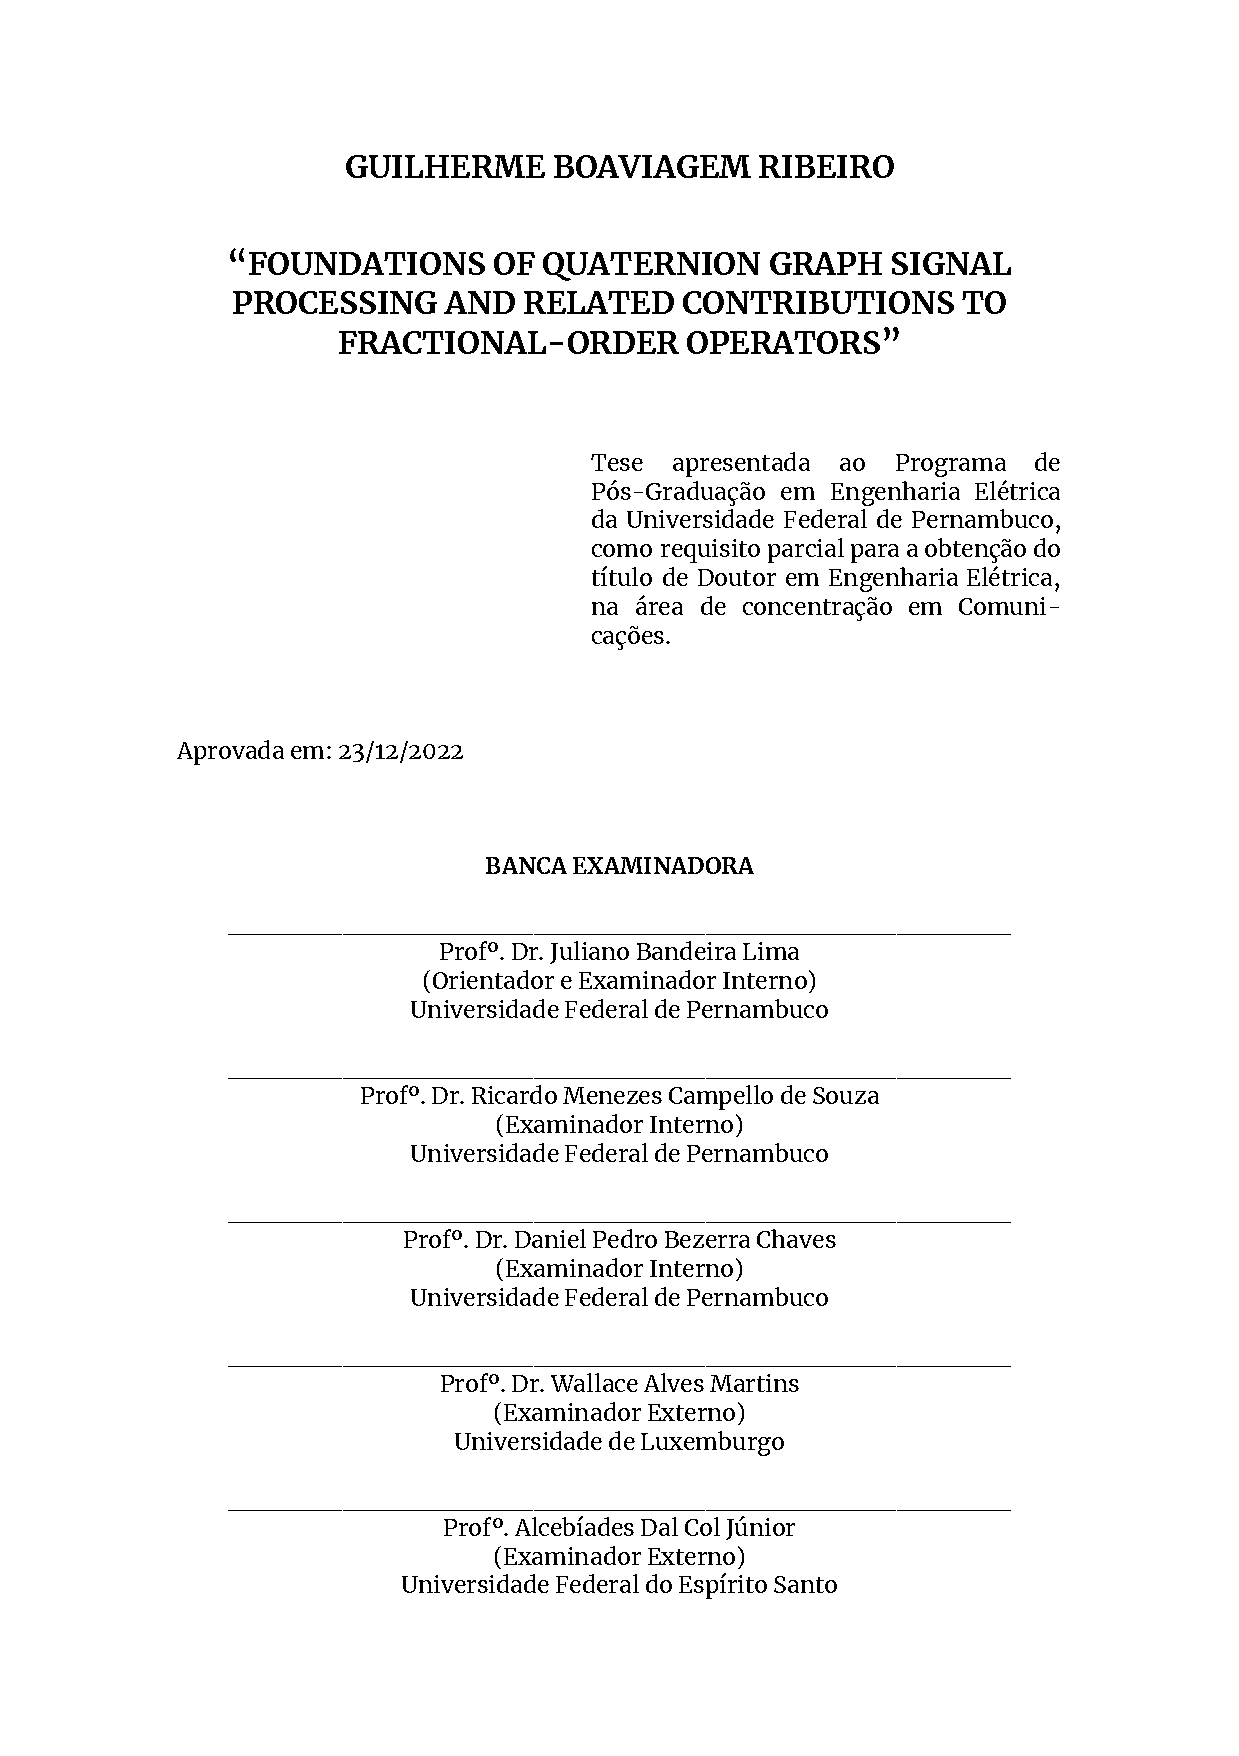
\includepdf[pages={1}]{./frontmatter/fichacatalografica.pdf}
    % 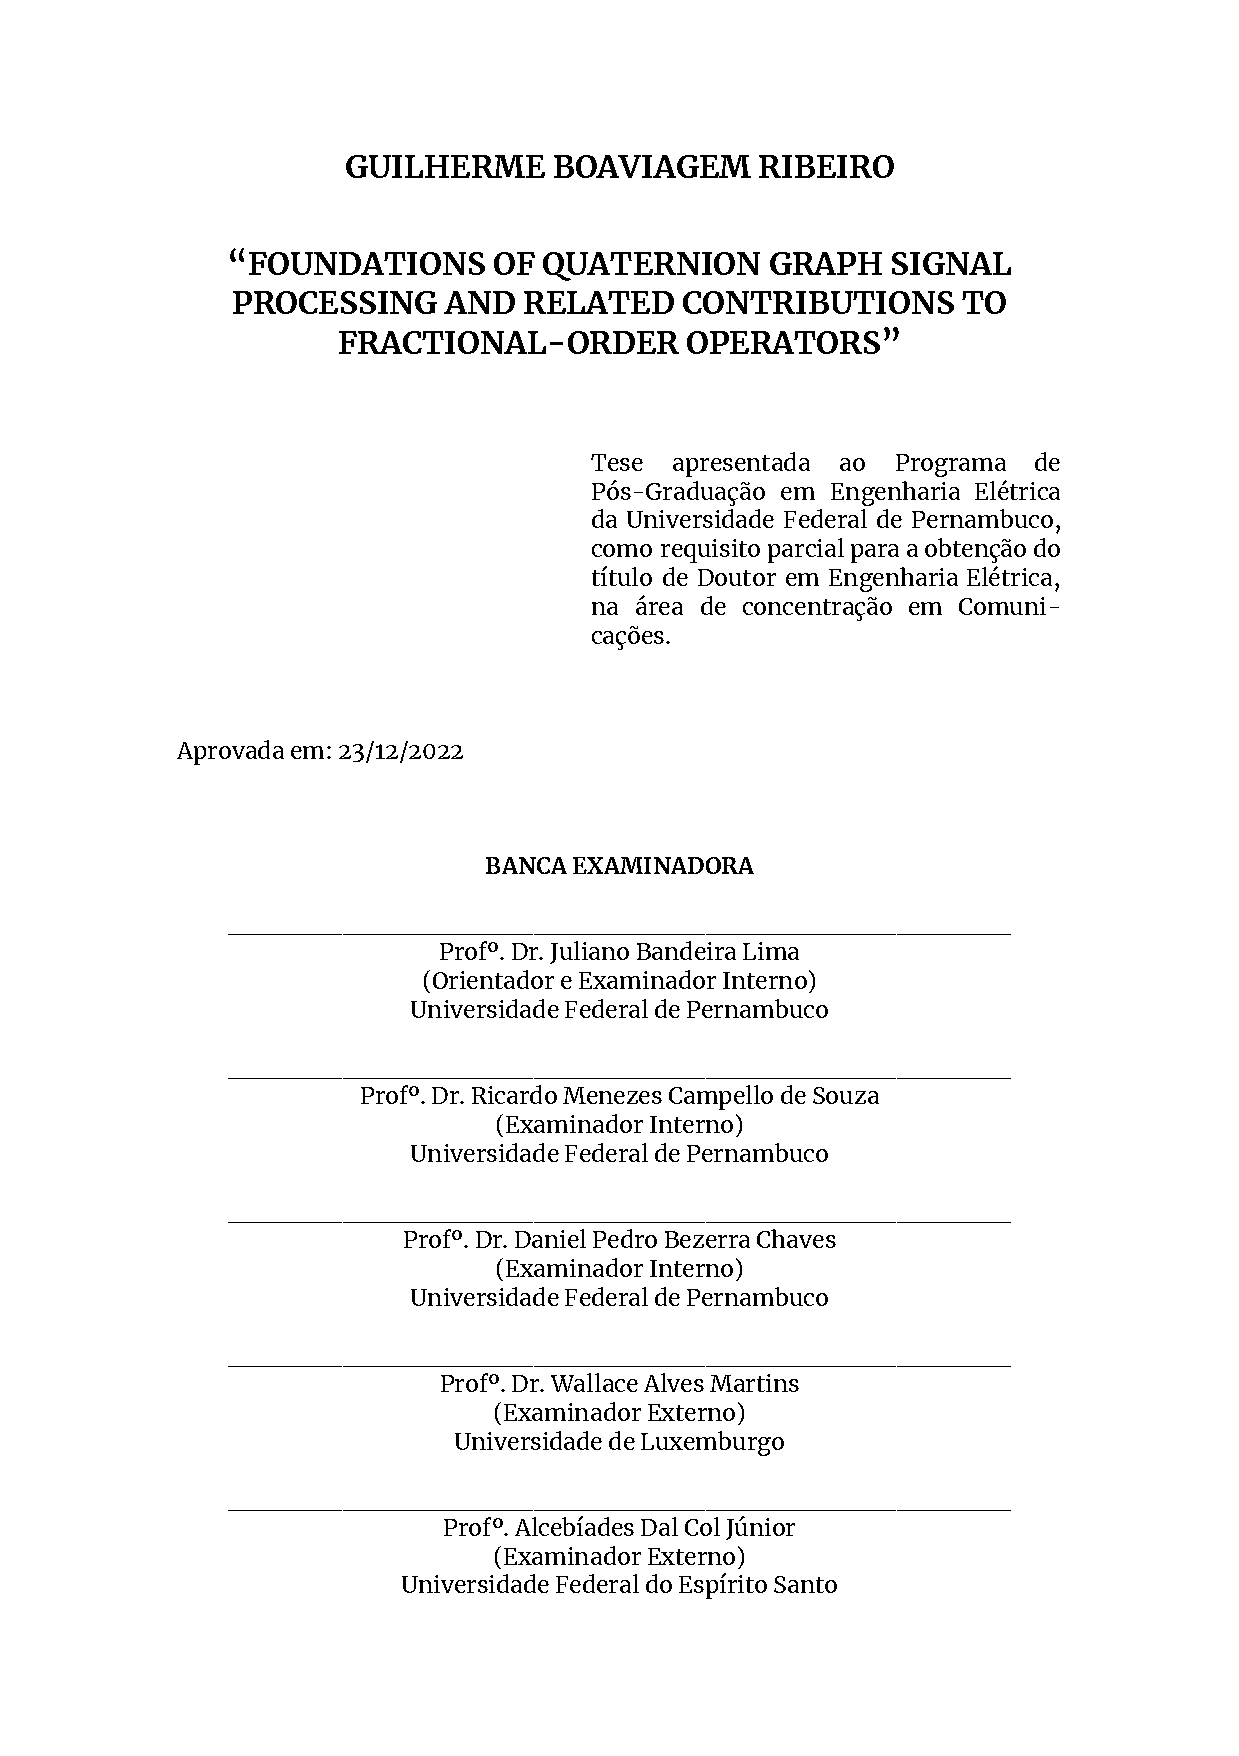
\includepdf[pages=-]{frontmatter/fichacatalografica.pdf}
% \end{fichacatalografica}

% \begin{fichacatalografica}
% 	\sffamily
% 	\vspace*{\fill}					% Posição vertical
% 	\begin{center}					% Minipage Centralizado
% 	\fbox{\begin{minipage}[c][8cm]{13.5cm}		% Largura
% 	\small
% 	\imprimirautor
% 	%Sobrenome, Nome do autor
	
% 	\hspace{0.5cm} \imprimirtitulo  / \imprimirautor. --
% 	\imprimirlocal, \imprimirdata-
	
% 	\hspace{0.5cm} \thelastpage p. : il. (algumas color.) ; 30 cm.\\
	
% 	\hspace{0.5cm} \imprimirorientadorRotulo~\imprimirorientador\\
	
% 	\hspace{0.5cm}
% 	\parbox[t]{\textwidth}{\imprimirtipotrabalho~--~\imprimirinstituicao,
% 	\imprimirdata.}\\
	
% 	\hspace{0.5cm}
% 		1. Palavra-chave1.
% 		2. Palavra-chave2.
% 		2. Palavra-chave3.
% 		I. Orientador.
% 		II. Universidade xxx.
% 		III. Faculdade de xxx.
% 		IV. Título 			
% 	\end{minipage}}
% 	\end{center}
% \end{fichacatalografica}
% ---

% ---
% Inserir errata
% ---
%\begin{errata}
%Elemento opcional da \citeonline[4.2.1.2]{NBR14724:2011}. Exemplo:
%
%\vspace{\onelineskip}
%
%FERRIGNO, C. R. A. \textbf{Tratamento de neoplasias ósseas apendiculares com
%reimplantação de enxerto ósseo autólogo autoclavado associado ao plasma
%rico em plaquetas}: estudo crítico na cirurgia de preservação de membro em
%cães. 2011. 128 f. Tese (Livre-Docência) - Faculdade de Medicina Veterinária e
%Zootecnia, Universidade de São Paulo, São Paulo, 2011.
%
%\begin{table}[htb]
%\center
%\footnotesize
%\begin{tabular}{|p{1.4cm}|p{1cm}|p{3cm}|p{3cm}|}
%  \hline
%   \textbf{Folha} & \textbf{Linha}  & \textbf{Onde se lê}  & \textbf{Leia-se}  \\
%    \hline
%    1 & 10 & auto-conclavo & autoconclavo\\
%   \hline
%\end{tabular}
%\end{table}
%
%\end{errata}
% ---

% ---
% Inserir folha de aprovação
% ---

% Isto é um exemplo de Folha de aprovação, elemento obrigatório da NBR
% 14724/2011 (seção 4.2.1.3). Você pode utilizar este modelo até a aprovação
% do trabalho. Após isso, substitua todo o conteúdo deste arquivo por uma
% imagem da página assinada pela banca com o comando abaixo:
%
% \begin{folhadeaprovacao}
% 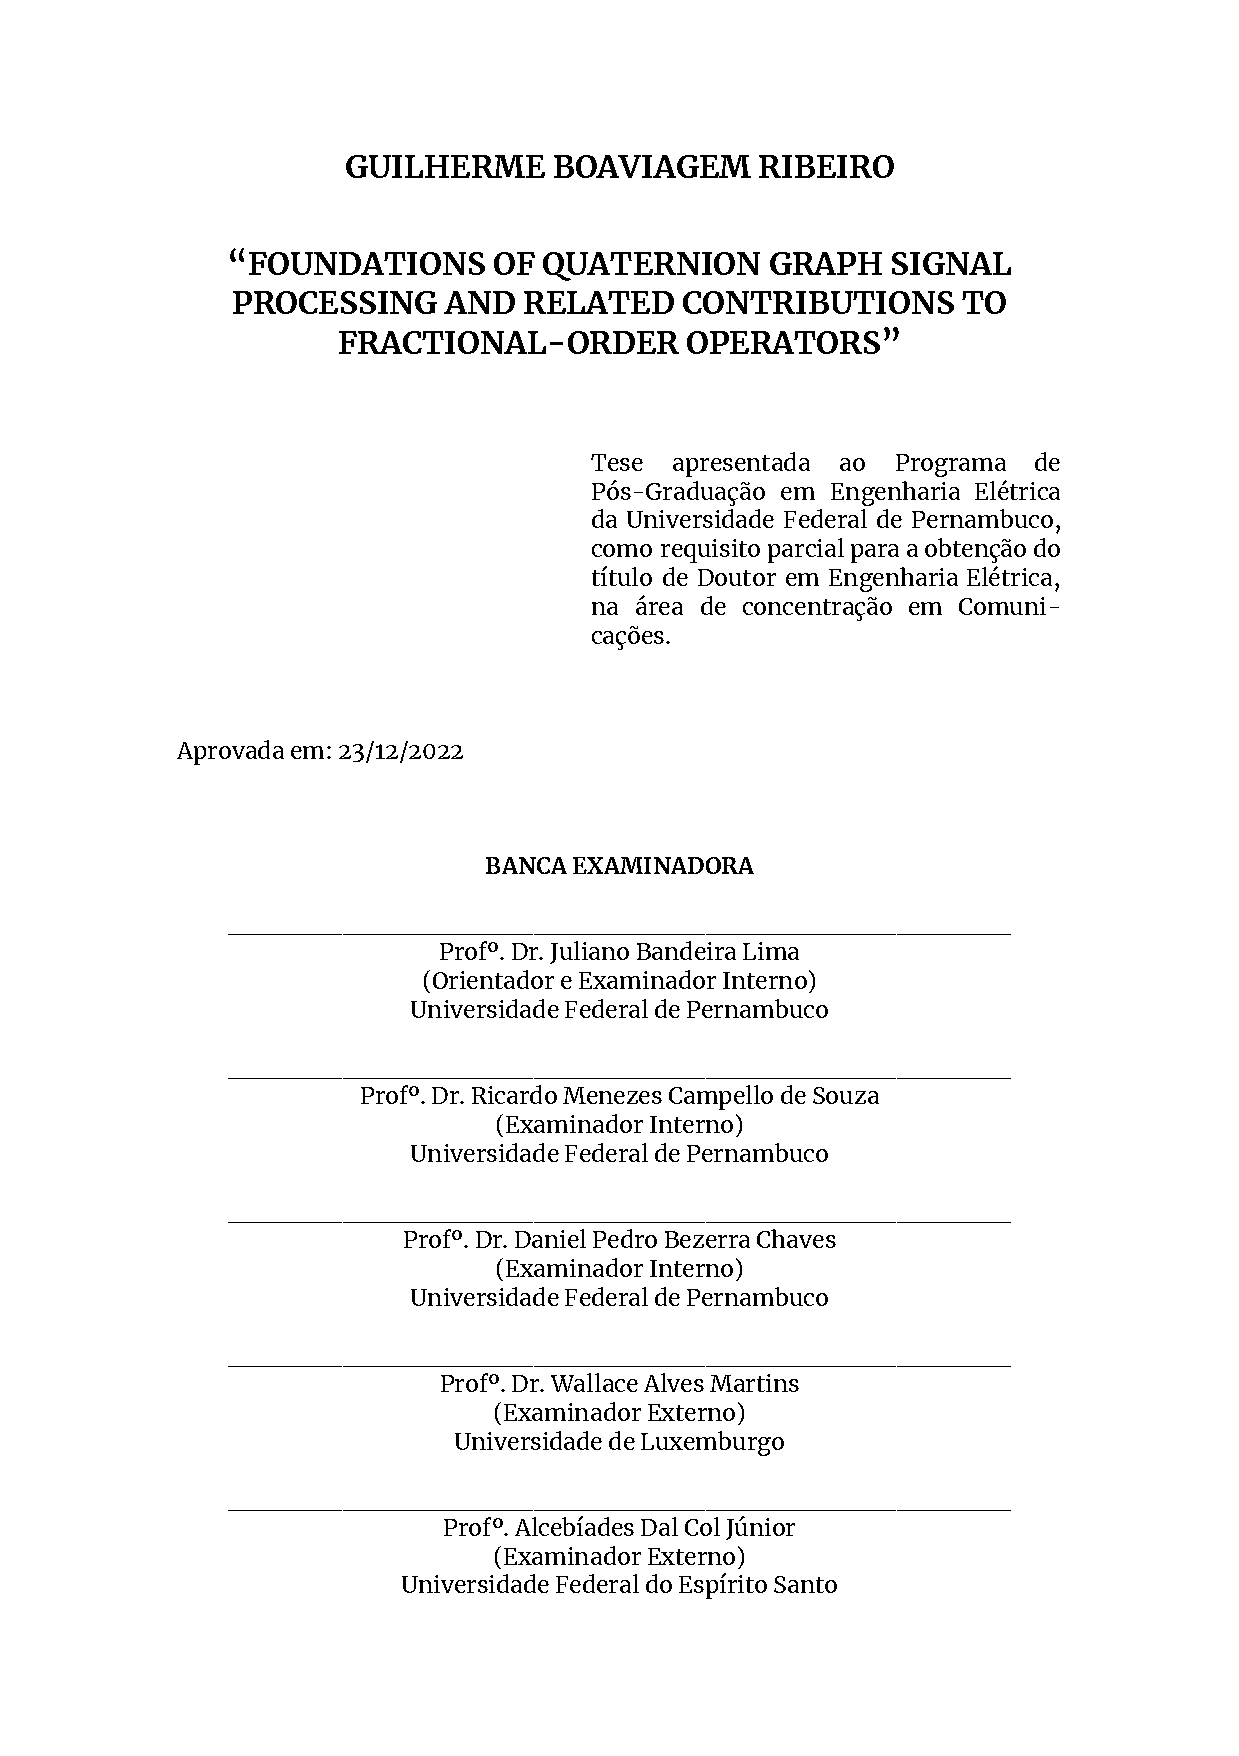
\includepdf[pages={1}]{./frontmatter/folha_de_aprovacao.pdf}
% \end{folhadeaprovacao}
%
\begin{folhadeaprovacao}
    \begin{center}
% {\ABNTEXchapterfont\large\imprimirautor}
\MakeUppercase{\rmfamily\mdseries\normalsize\imprimirautor}

\vspace*{\fill}\vspace*{\fill}
\begin{center}
    % \ABNTEXchapterfont\bfseries\Large\imprimirtitulo
    \MakeUppercase{\rmfamily\bfseries\normalsize\imprimirtitulo}
\end{center}
\vspace*{\fill}

\hspace{.45\textwidth}
\begin{minipage}{.5\textwidth}
    \imprimirpreambulo
\end{minipage}%
\vspace*{\fill}
\end{center}

This work received unconditioned approval in 23/12/2022 by the following doctoral committee:

\assinatura{\textbf{\imprimirorientador} \\ (Advisor and Internal Examiner) \\ Federal University of Pernambuco}
\assinatura{\textbf{Prof. Dr. Ricardo Menezes Campello de Souza} \\ (Internal Examiner) \\ Federal University of Pernambuco}
\assinatura{\textbf{Prof. Dr. Daniel Pedro Bezerra Chaves} \\ (Internal Examiner) \\ Federal University of Pernambuco}
\assinatura{\textbf{Prof. Dr. Wallace Alves Martins} \\ (External Examiner) \\ University of Luxembourg}
\assinatura{\textbf{Prof. Dr. Alceb\'iades Dal Col J\'unior} \\ (External Examiner) \\ Federal University of Esp\'irito Santo}
    
\begin{center}
% \vspace*{0.5cm}
{\large\imprimirlocal}
\par
{\large\imprimirdata}
% \vspace*{1cm}
\end{center}
\end{folhadeaprovacao}
% ---

\begin{dedicatoria}
    \vspace*{\fill}
\centering
\noindent
{To my wife, B\'arbara, and children, Rafael and Gianna.} \vspace*{\fill}
\end{dedicatoria}

\begin{agradecimentos}
    % !TEX root = ../thesis-example.tex
%
% \pdfbookmark[0]{Agradecimentos}{Agradecimentos}
% \chapter*{Agradecimentos}
% \label{sec:acknowledgement}
%\vspace*{-10mm}

\begin{openingquote}
    Let me stress this point: it is in the simplicity of your \emph{ordinary work}, in the monotonous details of each day, that you have to find the secret, which is hidden from so many, of something great and new: Love. \cite[n. 489]{escriva2016sulco}
\end{openingquote}

At the touch of Love, a divine Person who calls and moves the heart amidst daily activities, the feeling of gratitude is inevitable. Especially here, I thank for the graces granted to carry out this work and bear fruit with the time granted by Him. His kindness knows no end.

I also direct my deep and sincere gratitude to some people who were fundamental in making the development and completion of this work possible.

I thank B\'arbara, my wife, for being the occasion to find our deepest Love every day. In addition to sharing life and the future with me, her dedication in the small things made it possible for me to complete this journey.

I thank my parents and my brother for the education and example with which they nurtured me throughout my life. They gave me the possibility to be who I am, and for that, I will be eternally grateful. Also to my in-laws, sisters-in-law, and close friends, whose strong affection manifests itself in the continuous generosity and support they give to me and my family.

I also thank Prof. Juliano Bandeira, my advisor, who with incredible patience and clarity helped me rediscover the path of research when it seemed so forgotten and challenging. His guidance helped me see the way and gather strength for the last miles of this long-distance race.

I also thank Petrônio Braga and my colleagues at Neurotech for the conversations both inside and outside of work, which in one way or another helped me mature my perspective and not leave behind my academic vein.

Finally, I thank CAPES and the Office of Research and Graduate Studies (in portuguese, Pr\'o-reitoria de Pesquisa e P\'os-gradua\c c\~ao) at UFPE for the financial support during part of this research (under project n. 88882.380374/2019-01), and the Graduate Program in Electrical Engineering at UFPE for the opportunity granted.

\end{agradecimentos}

\begin{epigrafe}
    \vspace*{\fill}
\begin{openingquote}
Algebra is generous, she often gives more than is asked of her.
\cite{bulletinams}    
\end{openingquote}
\end{epigrafe}
% ---

%
%% resumo em inglês
\begin{resumo}[Abstract]
    \begin{otherlanguage*}{english}
    
% !TEX root = ../thesis-example.tex
%
\pdfbookmark[0]{Abstract}{Abstract}
\chapter*{Abstract}
\label{sec:abstract}
%\vspace*{-10mm}

The field signal processing, at its core, is concerned with exploring how different representations of a signal may provide useful ways of manipulating it. These representations may arise from a change in the subjacent algebra over which the signal samples are defined, for example when embedding three- and four-dimensional signals into the quaternion space; or maybe from a different model of the signal domain, as it happened with the development of graph signal processing to deal with network-like data; or even by exploring new linear transforms that map the signal onto a domain in which tasks such as compression, filtering or feature extraction are easier or more efficient.

This thesis traverses exactly through these paths, aiming at answering the question of how to extend graph signal processing to the case in which signals and edge weights are quaternion-valued. It proposes a new set of tools which are a basis for what may be called Quaternion Graph Signal Processing (QGSP) and, as byproducts of the research journey, it contributes to the field of fractional transforms in two fronts: by proposing a new approach to the fractionalization of the quaternion discrete Fourier transform (QDFT), alongside the proposition of its multiparametric version, and by proposing a new fractional graph shift operator (GSO).

As highlights of the main results, we can mention: (1) the polynomial representation of the fractional GSO for arbitrary graphs was obtained, and it was shown that its use in filter design of FIR LSI filters improve the overall filter quality for a given filter length; (2) the new multiparametric fractional QDFT was used to create a holistic encryption scheme for color images with opacity layer, which was shown to provide satisfactorily large key space and key sensitivity; and (3) the main aspects of spectral analysis, filtering and compression in the context of QGSP were formulated, along extensive practical examples on real-world data computed through a custom-made and open-source Python package.
\vspace{1em}

\noindent
\textbf{Keywords}: quaternions, fractional quaternion discrete Fourier transform, fractional graph shift operator, quaternion graph signal processing.

    \end{otherlanguage*}
\end{resumo}

\begin{resumo}[Resumo]
    \begin{otherlanguage*}{portuguese}
    
% !TEX root = ../thesis-example.tex
%
% \pdfbookmark[0]{Abstract}{Abstract}
% \chapter*{Abstract}
% \label{sec:abstract}
%\vspace*{-10mm}

A área de Processamento de Sinais, em sua essência, preocupa-se em explorar como diferentes representações de um sinal podem fornecer maneiras úteis de manipulá-lo. Essas representações podem surgir, por exemplo, a partir de uma mudança na álgebra subjacente sobre a qual as amostras do sinal são definidas, como ocorre ao representar sinais de três ou quatro dimensões como vetores de um espaço vetorial quaterniônico. Outras representações podem advir de mudanças no domínio do sinal, como ocorreu com o desenvolvimento do processamento de sinais de grafos, para lidar com sinais estruturados em rede; ou ainda podem vir da exploração de novas transformadas lineares que mapeiam o sinal em um domínio em que tarefas como compressão, filtragem ou extração de recursos sejam mais fáceis ou eficientes.
Esta tese desenvolve-se exatamente por esses caminhos, visando responder à pergunta de como estender o processamento de sinais sobre grafos para o caso em que os sinais e pesos das arestas são quaterniônicos. Propõe-se um novo conjunto de ferramentas que são a base do que pode ser chamado de Processamento de Sinais Quaterniônicos sobre Grafos (QGSP, \emph{quaternion graph signal processing}) e, como subprodutos da jornada de pesquisa, contribui-se para o campo das transformadas fracionárias em duas frentes: propondo uma nova abordagem para a fracionalização da transformada discreta de Fourier quaterniônica (QDFT, \emph{quaternion discrete Fourier transform}), juntamente com a proposta de sua versão multiparamétrica, e propondo um novo operador de deslocamento sobre grafo fracionário (GSO, \emph{graph shift operator}).
Entre os principais resultados, podemos mencionar: (1) a representação polinomial do GSO fracionário para grafos arbitrários foi obtida, e foi demonstrado que seu uso no projeto de filtros de resposta finita de impulso e lineares e invariantes a deslocamento (FIR LSI, \emph{finite impulse response and linear and shift-invariant}) melhora a qualidade geral do filtro para um determinado comprimento de filtro; (2) a nova QDFT fracionária multiparamétrica foi usada para criar um esquema de criptografia holística para imagens coloridas com camada de opacidade, que fornece um espaço de chave satisfatoriamente grande e com grande sensibilidade à mudança de chave; e (3) os principais aspectos da análise espectral, filtragem e compressão no contexto do QGSP foram formulados, juntamente com extensos exemplos práticos em dados do mundo real calculados por meio de um pacote Python personalizado e de código aberto.
\vspace{1em}

\noindent
Palavras-chave: quatérnios; transformada discreta de Fourier quaterniônica fracionária; operador de deslocamento de grafo fracionário; processamento de sinal de grafo quaterniônico.
    \end{otherlanguage*}
\end{resumo}

% resumo em francês 
%\begin{resumo}[Résumé]
%\begin{otherlanguage*}{french}
%Il s'agit d'un résumé en français.
%
%\textbf{Mots-clés}: latex. abntex. publication de textes.
%\end{otherlanguage*}
%\end{resumo}

% resumo em espanhol
%\begin{resumo}[Resumen]
%\begin{otherlanguage*}{spanish}
%Este es el resumen en español.
%
%\textbf{Palabras clave}: latex. abntex. publicación de textos.
%\end{otherlanguage*}
%\end{resumo}
% ---

% ---
% inserir lista de ilustrações
% ---
\pdfbookmark[0]{\listfigurename}{lof}
\listoffigures*
\cleardoublepage
% ---

% ---
% inserir lista de quadros
% ---
%\pdfbookmark[0]{\listofquadrosname}{loq}
%\listofquadros*
%\cleardoublepage
% ---

% ---
% inserir lista de tabelas
% ---
%\pdfbookmark[0]{\listtablename}{lot}
%\listoftables*
%\cleardoublepage
% ---

% ---
% inserir lista de abreviaturas e siglas
% ---
\begin{siglas}
    \pdfbookmark[0]{Abbreviations}{Abbreviations}
\chapter*{List of abbreviations}
\label{sec:acronimos}
%\vspace*{-10mm}

\begin {description}[leftmargin=8em,style=nextline]
\item[DSP] Digital Signal Processing.
\item[LTI] Linear and Time-invariant.
\item[FIR] Finite Impulse Response.
\item[DFT] Discrete Fourier Transform.
\item[QFT] Quaternion Fourier Transform.
\item[FrFT] Fractional Fourier Transform.
\item[FrDFT] Fractional Discrete Fourier Transform.
\item[FrQDFT] Fractional Quaternion Discrete Fourier Transform.
\item[MFrQDFT] Multi-parametric Fractional Quaternion Discrete Fourier Transform.
\item[GSP] Graph Signal Processing.
\item[GSO] Graph Shift Operator.
\item[QGSP] Quaternion Graph Signal Processing.
\item[LSI] Linear and Shift-invariant.
\item[NMSE] Normalized Mean Squared Error.
\end {description}


\end{siglas}
% ---

% ---
% inserir lista de símbolos
% ---
\begin{simbolos}
    \pdfbookmark[0]{List of symbols}{symbols}
\chapter*{List of symbols}
\label{sec:symbols}
%\vspace*{-10mm}


\begin{description}[leftmargin=8em,style=nextline]
    \item[$ \mathbf{A} $] Graph weighted adjacency matrix.
    \item[$ \mathbf{L} $] Graph Laplacian matrix.
    \item[$ \mathbf{\Lambda}, \mathbf{J} $] Respectively the eigenvalue matrix (if it exists) and the Jordan matrix of the graph adjacency matrix.
    \item[$ \mathbf{V} $] The (possibly generalized) eigenvector matrix of the graph adjacency matrix.
    \item[$\mathcal{R}e \{ x \}$] Real part of the complex number $x$.
    \item[$\mathcal{I}m \{ x \}$] Imaginary part of the complex number $x$.
    \item[$ \overline{x} $] Conjugate of the complex (or quaternion) $x$. If vectors or matrices are used instead of $x$, the conjugation is realized in each of its entries.
    \item[$\mathbf{M}^T$] Transpose of the matrix $\mathbf{M}$.
    \item[$\mathbf{M}^H$] Conjugate transpose of the matrix $\mathbf{M}$.
    \item[$\mathbb{R}$, $\mathbb{C}$ \textnormal{and} $\mathbb{H}$] Respectively the set of real, complex and (Hamiltonian) quaternion numbers. By association, we may also refer to the respective (skew-)field.
    \item[$\mathbb{F}^n$] Set of the vectors of length $n$ with entries in the (possibly skew) field $\mathbb{F}$.
    \item[$ | \cdot | $] Modulus of a real, complex or quaternion number.
    \item[$ \rchi_A $] Complex adjoint of the quaternion matrix $ \mathbf{A} $.
    \item[$ S(q) $] Scalar part of the quaternion $q$.
    \item[$ \qV(q) $] Vector part of the quaternion $q$.
    \item[$ \qV(\mathbb{H}) $] Set of all pure quaternions (i.e. with null scalar part).
    \item[$ \qi $, $ \qj $ \textnormal{and} $ \qk $] Unit pure quaternions which constitute the canonical basis for the set of pure quaternions.
    \item[$ \mathbb{C}_{\qmu}$] Set of numbers $\{ a + b\qmu \ | \ a, b \in \mathbb{R} \}$ with $\qmu \in \qV(\mathbb{H})$ and $|\qmu| = 1$, isomorphic to the complex numbers.
    \item[$ \Vert \mathbf{x}\Vert_p $] $ \ell_p $-norm of the vector $\mathbf{x} \in \mathbb{C}^n$, defined as $\left(\sum_{k=0}^{n-1} |x_k|^p\right)^{1/p}$.
\end{description}
\end{simbolos}


% ---

% ---
% inserir o sumario
% ---
\pdfbookmark[0]{\contentsname}{toc}
\tableofcontents*
\cleardoublepage
% ---



% ----------------------------------------------------------
% ELEMENTOS TEXTUAIS
% ----------------------------------------------------------
\textual

\chapter{Introduction}
\label{ch:Intro}

Signal processing often interweaves pure mathematics and engineering. One of its concerns is the \textit{representation} of signals (functions) and how different representations may be explored to better manipulate such signals. The spectral analysis via Fourier and similar transforms, for instance, aims to project the signal onto a domain in which the energy support is more compact (compression), or in which some frequencies are easier to be removed (filtering), or yet in which some relevant features may be created (feature engineering for machine learning problems), among others \cite{oppenheim1999discrete, rabiner2010theory, graf2015features, vergin1999generalized}.

One way to explore different signal representations is to alter the algebra over which its sample values are defined. That is the case with number-theoretic transforms \cite{lima2011finite,blahut2010fast,pedrouzo2017number,chandra2014exact}, which deal only with finite algebraic structures instead of the usual complex (e.g. Fourier transform) or real fields (e.g. cosine transform). As the underlying algebra is extended, e.g. going from $ \mathbb{R} $ to $ \mathbb{C} $, it is possible to process signals with more information per sample. Such was the motivation behind Sangwine's \cite{sangwine1996fourier} discrete version of a family of bidimensional transforms over the \textit{quaternions}, previously created by Ell \cite{ell1993quaternion}: to exploit this class of hypercomplex numbers with four real components to perform holistic color image processing. Upon mapping each color channel inside a pixel into an imaginary component of a quaternion number, the color image may be processed as a single 2D signal -- instead of three, one per color channel. The holistic (as opposed to separate) processing of the color signal allows to explore the correlation and coupling between the channels, and this is generally the advantage intended when using quaternion signal processing to handle three- or four-dimensional data \cite{took2008quaternion}. Computationally, the spectral decomposition requires only two complex discrete Fourier transforms (DFTs), instead of three (one per color channel). Ever since, quaternion transforms have been employed not only on color image processing \cite{ell2007hypercomplex,chen2018quaternion,li2013quaternion,evans2000hypercomplex}, but also on other tasks such as bivariate signal analysis \cite{flamant2017spectral,flamant2017time,flamant2018complete}.

Algebra extensions change the signal representation by looking at the signal \textit{samples} but, reminding the signal is nothing more than a function, one may also shift the attention to the \textit{domain}. In fact, such a reflection has led to the creation of graph signal processing (GSP). This field, which emerged in the last decade, is concerned with extending the concepts of classical discrete signal processing (DSP) to the case in which the signal samples \textit{reside in graph vertices}. It coincides with the classical case of discrete-time domain (for periodic signals) when using a path or ring graph -- depending on the graph shift operator (GSO) at hand, as will soon be clear -- with equally weighted edges. The \textit{signal}, therefore, is a mapping from the vertex set to the real (or complex) numbers, and the fixed sampling frequency is represented as graph edges having the same weights (i.~e., as if the samples were at fixed ``distances'', one could say). GSP deals with the consequences of conecting more vertices in this graph, moving from the queue-shaped domaing into an arbitrary network. Many definitions from classical digital signal processing (DSP) have already found their way into GSP, thanks to the contributions of many scholars who proposed ways to implement filtering \cite{sandryhaila2013filters}, linear transforms \cite{sandryhaila2013gft,sardellitti2017graph}, interpolation \cite{segarra2015interpolation}, sampling theorem on graphs \cite{wang2015generalized,chen2016signal,tsitsvero2016signals}, among others.

The endeavor to experiment with different algebras or domain topologies has primarily theoretical motivations, but often reveal new solutions to real world problems. Taking GSP for instance, its applications spread from coding \cite{su2017graph} and light field image super resolution schemes \cite{rossi2017graph}, to regulatory genetic networks, in which graph-based methods have already improved three state-of-the-art network inference schemes \cite{pirayre2015brane,pirayre2017brane}, also reaching recommender systems, both collaborative filtering and content-based, using regularization of graph total variation \cite{benzi2016song}, semi-supervised learning through adaptive graph filters \cite{chen2014semi}, community detection using graph wavelets \cite{tremblay2014graph}, among others. The latter examples hint at the intersection between GSP and the fields of data science and machine learning -- well established and highly active, both in Academia and industry --, to the point where we can join Benjamin Ricaud and say that \emph{Fourier could very well be, today, a data scientist} \cite{ricaud2019fourier}.

As happened to GSP, the study of quaternion-valued signal processing has also found applications. Beyond the already mentioned use in manipulating color image and bivariate signals, the work on adaptive quaternion filters has been useful, for example, in wind profile prediction \cite{jiang2014general}. Or yet the remarkable union of graphs and quaternions in the work by \cite{zhang2019quaternion} -- the only one the author is aware of --, in which quaternion embeddings are used to form a low dimensional representation of entities and relations in knowledge graphs.

In this context, this doctoral research tackles the following problem: is it possible to perform signal processing having quaternion-valued samples residing on graphs with quaternion-weighted edges? What limitations and new possibilites may arise when exploring what we may call \textit{quaternion graph signal processing} (QGSP)? That is the spark which ignited the studies and results presented in the following chapters.

As it will become clear to the reader, however, the pathway to the basis of QGSP was not a straight line. Sometimes what seemed to be dead ends emerged, and during the reflections upon ways to bypass them, other interesting results started to appear. For example, it was certain from the beginning that the problem of eigendecomposing quaternion matrices would be at the heart of QGSP, since the very definition of a graph signal spectrum requires the eigenvalues and eigenvectors of a GSO (e.g. the adjacency matrix), which is a quaternion matrix. Since it took a while to make progress with general graph matrices, it seemed promising to investigate the quaternion discrete Fourier transform (QDFT); after all, ring graphs should have the graph Fourier transform (GFT) and the classical discrete Fourier transform (DFT) coinciding. By looking at the QDFT matrix, however, a new way to diagonalize it was found and a new multiparametric fractional QDFT was proposed. When shifting the focus to the graph domain, revisiting the study of graph shift operators and their spectral decomposition, interesting results regarding the fractional GSO were discovered. For instance, this new operator acts as a graph filter, and its polynomial representation was fully determined, demonstrating that it can be implemented as a linear and shift-invariant (LSI) graph filter. These unforeseen results are featured in this document, as they paved the way for the foundations of QGSP.

\section{Organization}

This doctoral dissertation is organized as follows. Chapters \ref{ch:reviewQuat} and \ref{ch:reviewGSP} bring a diverse set of concepts and results from the literature, providing the reader with a sufficient understanding of the quaternion algebra and quaternion Fourier transform (the former), and signal processing from the perspective of graph signals and fractional-order operators (the latter).
Chapter \ref{ch:FrGSO} presents the new fractional graph shift operator, commenting on its properties and applications.
In Chapter \ref{ch:FrQDFT}, a study on the fractionalization of the QDFT is presented, with a new method being proposed, alongside a multiparametric version of the fractional-order transform.
The foundations of QGSP are finally presented in Chapter \ref{ch:QGSP}, with discussions and a few applications with both toy and real world datasets.
The thesis closes with concluding remarks and future works in Chapter \ref{ch:conclusion}. Appendix \ref{ch:AppendixA} leads the reader through the demonstration of a relation between systems of quaternion and complex linear equations, useful for a central theorem presented in Chapter \ref{ch:reviewQuat}. As a final note, the reader may notice that many concepts in the chapters dedicated to basic literature review are presented outside formal theorems and propositions. Far from being a conscious decision from the beginning, it happened as an unconscious stylistic choice, prioritizing a steady flow of writing to the detriment of mathematical formalism. The citations found along the text will provided the adequate formal treatment to the interested readers.

\section{Contributions}
The contributions of this doctorate research, featured in this doctoral dissertation, are:

\vspace{-1em}
\begin{itemize}[noitemsep]
    \item The proposition and discussion of the fractional graph shift and its application on improving least-squares approximation of linear and shift-invariant ideal filters.
    \item A theorem which proves that the QDFT and the DFT share symmetric eigenvalues, and which enables a novel approach to fractionalizing the quaternion discrete Fourier transform (QDFT).
    \item The definition of a multiparametric fractional QDFT and its application in a novel image encryption scheme.
    \item The proposition of quaternion graph signal processing (QGSP), a new tool designed for specialized scenarios in which both the signal samples and their quantifiable relationship may be expressed as quaternions (thus having at most four dimensions or information sources).
    \item \texttt{gspx},\footnote{The library is available as an open repository: \url{https://github.com/gboaviagem/gspx}.} an open-source Python library with implementation of the core concepts from QGSP.
\end{itemize}
\vspace{-1em}
\section{Publications}

This work has so far published two papers in international journals, one in a global conference, and a book. The paper \textit{``Eigenstructure and fractionalization of the quaternion discrete Fourier transform''}, published in Optik, contains the results of Chapter \ref{ch:FrQDFT}. The 10th volume of IEEE Access received the work \textit{``On the Fractionalization of the Shift Operator on Graphs''}, containing the results of Chapter \ref{ch:FrGSO}. As the understanding of GSP matured during the doctorate research, the author contributed with some chapters to the book ``Processamento de Sinais sobre Grafos: Fundamentos e Aplica{\c c}{\~o}es'', published in the \textit{Notas em Matem\'atica Aplicada} series from the Brazilian society \textit{Sociedade Brasileira de Matemática Aplicada e Computacional (SBMAC)}.

The paper \emph{``The Cosine Number Transform: A Graph Signal Processing Approach''}, presented in the 2019 edition of GlobalSIP, was created during short attempts to further generalize GSP to other algebraic structures, in particular to graphs with edge weights in finite fields. However, it has not evolved into more substantial findings and thus, although it stems from this work, it is not featured in this dissertation. The full references of the mentioned publications are:

\vspace{-1em}
\begin{itemize}[noitemsep]
    % Citing in MLA Format, extracted from Google Scholar.
    \item Ribeiro, Guilherme and Lima, Juliano. ``The Cosine Number Transform: A Graph Signal Processing Approach''. \textit{2019 IEEE Global Conference on Signal and Information Processing (GlobalSIP)}. IEEE, 2019. DOI: \href{https://doi.org/10.1109/GlobalSIP45357.2019.8969165}{10.1109/GlobalSIP45357.2019.8969165}

    \item Ribeiro, Guilherme B., and Lima, Juliano B. ``Eigenstructure and fractionalization of the quaternion discrete Fourier transform''. \textit{Optik} 208 (2020): 163957. DOI: \href{https://doi.org/10.1016/j.ijleo.2019.163957}{10.1016/\-j.ijleo.2019\-.163957}.

    \item Ribeiro, Guilherme B., José R. De Oliveira Neto, and Lima, Juliano B. ``On the Fractionalization of the Shift Operator on Graphs''. \textit{IEEE Access} 10 (2022): 16468-16478. DOI: \href{https://doi.org/10.1109/ACCESS.2022.3149755}{10.1109/ACCESS.2022.3149755}.

    \item Lima, Juliano, et al. \textit{Processamento de Sinais sobre Grafos: Fundamentos e Aplica{\c c}{\~o}es}. Notas em Matem\'atica Aplicada, v. 92. Sociedade Brasileira de Matemática Aplicada e Computacional (SBMAC), 2022.
\end{itemize}

\section{Notation}
The use of symbols is a great way to communicate ideas concisely. However, instead of improving communication, they may make it cumbersome or even not communicate at all if the reader is not adequately familiar with them. Let us go through the main notation in this doctoral dissertation, to avoid confusion instead of clarity.

Simple numbers, either real-, complex- or quaternion-valued, are represented in italics, as in $q$. Special treatment is given to unit pure quaternions, represented in bold italics, e.g. $\qi$, $\qnu$. Numerical sets (and the related fields or skew-fields) are denoted using blackboard bold face (such as $\mathbb{R}$). Vectors and matrices are written with bold face: the former with lower case (e.g. $\mathbf{v} \in \mathbb{R}^{n}$), and the latter with upper case (e.g. $\mathbf{V} \in \mathbb{R}^{n \times n}$).

The function $\mathrm{diag}(\cdot)$ has context-dependent meaning: when the argument is a matrix, it returns the main diagonal as a column vector; whereas when it is a vector, it produces a diagonal matrix with this vector in its main diagonal. The symbol $\overset{\Delta}{=}$ represents \textit{equality by definition}.

The \textit{symplectic decomposition} of a quaternion number $q$ (or, by extension, of a quaternion-valued vector or matrix) will be \textit{usually} represented as $q = q_1 + q_2 \qj$, with subscripts $1$ and $2$ indicating the simplex and perplex components. When there is risk of mistaking the subscripts for indices (e.g. in summation), the alternative (more bulky) notation will employ superscripts $^{(s)}$ and $^{(p)}$, as in $q = q^{(s)} + q^{(p)} \qj$.

\chapter{A review on quaternion algebra and its Fourier transform}
\label{ch:reviewQuat}

\begin{openingquote}
    And here there dawned on me the notion that we must admit, in some sense, a fourth dimension of space for the purpose of calculating with triples... An electric circuit seemed to close, and a spark flashed forth.
    \cite[quoting directly Sir William Hamilton]{van1976hamilton}
\end{openingquote}


In 1833, at the age of 28, Willian Rowan Hamilton presented to the Royal Irish Academy (RIA) a work in which complex numbers were treated as ordered pairs of real numbers, given the appropriate definition of operations.\footnote{The results were published in 1837, in the paper \emph{Theory of Conjugate Functions, or Algebraic Couples; with a Preliminary and Elementary Essay on Algebra as the Science of Pure Time} \cite{hamilton1837theory}.} In the following years, he struggled to extend the complex field into a normed division algebra over triples, but soon realized that, as much as his attempts were inventive, the resulting algebra\footnote{An \textit{algebra over a field}, or simply \textit{algebra}, is a vector space over a field with a bilinear multiplication (that is, the multiplication distributes over the addition and the associativity is valid for multiplication) \cite{schafer1955introduction}.} was not closed under multiplication. We can see this through a simple example \cite{santos2011algebra}: let it be the set $\mathbb{F} = \{ a + b \qi + c \qj  \ | \ (a, b, c) \in \mathbb{R}^3\}$, with $\qi^2 = \qj^2 = -1$ and $\qi \neq \qj$. Since $\qi, \qj \in \mathbb{F}$, so there should exist $x, y, z \in \mathbb{R}$ so that
\begin{equation}
    \qi \qj = x + y \qi + z \qj.
    \label{eq:demonstration01}
\end{equation}

Multiplying by $\qi$ both sides of the equation,
\begin{equation}
    \qi^2 \qj = \qi x + \qi^2 y + z (\qi \qj),
\end{equation}
and using (\ref{eq:demonstration01}) it yields,
\begin{equation}
    - \qj = \qi x - y + z (x + y \qi + z \qj)
    \iff
    (zx - y) + \qi (x + zy) + \qj (z^2 + 1) = 0.
\end{equation}
That is: $z \notin \mathbb{R}$ and $ \qi \qj \notin \mathbb{F} $, proving that such algebraic structure is not closed under multiplication.

Only a decade later, in 1843, while walking by the roads in Dublin toward the RIA, ``an electric circuit seemed to close, and a spark flashed forth,'' as he would say. He had conceived the four-dimensional structure required to the desired algebra, creating the quaternions. Moved by excitement, he craved on the stone below Broome Bridge, in Cabra (Dublin), the equations that define the relations between the canonical basis elements of quaternions.\footnote{Close to the original site of the inscriptions, the RIA placed a commemorative plaque in 1958, with the same writings.} This creation, made possible by an insight in 1843, is found accross most of this work. The following sections lead the reader through the foundations of quaternion algebra and quaternion signal analysis.


\section{Introduction to the quaternion algebra}

Quaternions are numbers $q \in \mathbb{H}$ in the form
\begin{equation}
    q = a + b\qi + c\qj + d\qk,
    \label{eq:q}
\end{equation}
in which $a, b, c, d \in \mathbb{R}$, holding true the fundamental relations:
\begin{equation}
    \label{eq:fund_rel}
    \begin{aligned}
        \qi ^2 = \qj^2 & =\qk^2 = \qi \qj \qk = -1.
    \end{aligned}
\end{equation}

The multiplication rules between  $ \qi $, $ \qj $ and $ \qk $ follow directly from (\ref{eq:fund_rel}), resembling those between orthonormal basis vectors from $ \mathbb{R}^3 $ and the vector product: the product between two of them yields the third, the sign being determined from the operands order. For instance, to find the result of $ \qi \qj $ one may start from (\ref{eq:fund_rel}) and write
\begin{equation}
    \begin{aligned}
        \qi \qj \qk                         & = -1   \\
        \qi \qj \underbrace{\qk \qk}_{= -1} & = -\qk \\
        \qi \qj                             & = \qk.
    \end{aligned}
\end{equation}
Similarly, to find $ \qj \qi $,
\begin{equation}
    \begin{aligned}
        \qi \qj \qk     & = -1        \\
        \qi \qi \qj \qk & = -\qi      \\
        - \qj \qk       & = - \qi     \\
        \qj \qj \qk     & =  \qj \qi  \\
        - \qk           & =  \qj \qi. \\
    \end{aligned}
\end{equation}
Fig. \ref{fig:quatmult} depicts the order in which the product between any pair in the triplet $ \qi $, $ \qj $ and $ \qk $ yields the third one, with positive sign. All three units commute with real numbers. The most relevant consequence, therefore, of (\ref{eq:fund_rel}), is that the quaternion product is \textit{noncommutative}. In fact, it is the first example of noncommutative normed division algebra in history \cite{kleiner2007history}.

\begin{figure}
    \centering
    \caption{Illustration of the multiplication rule between the imaginary units $ \qi $, $ \qj $ and $ \qk $.}
    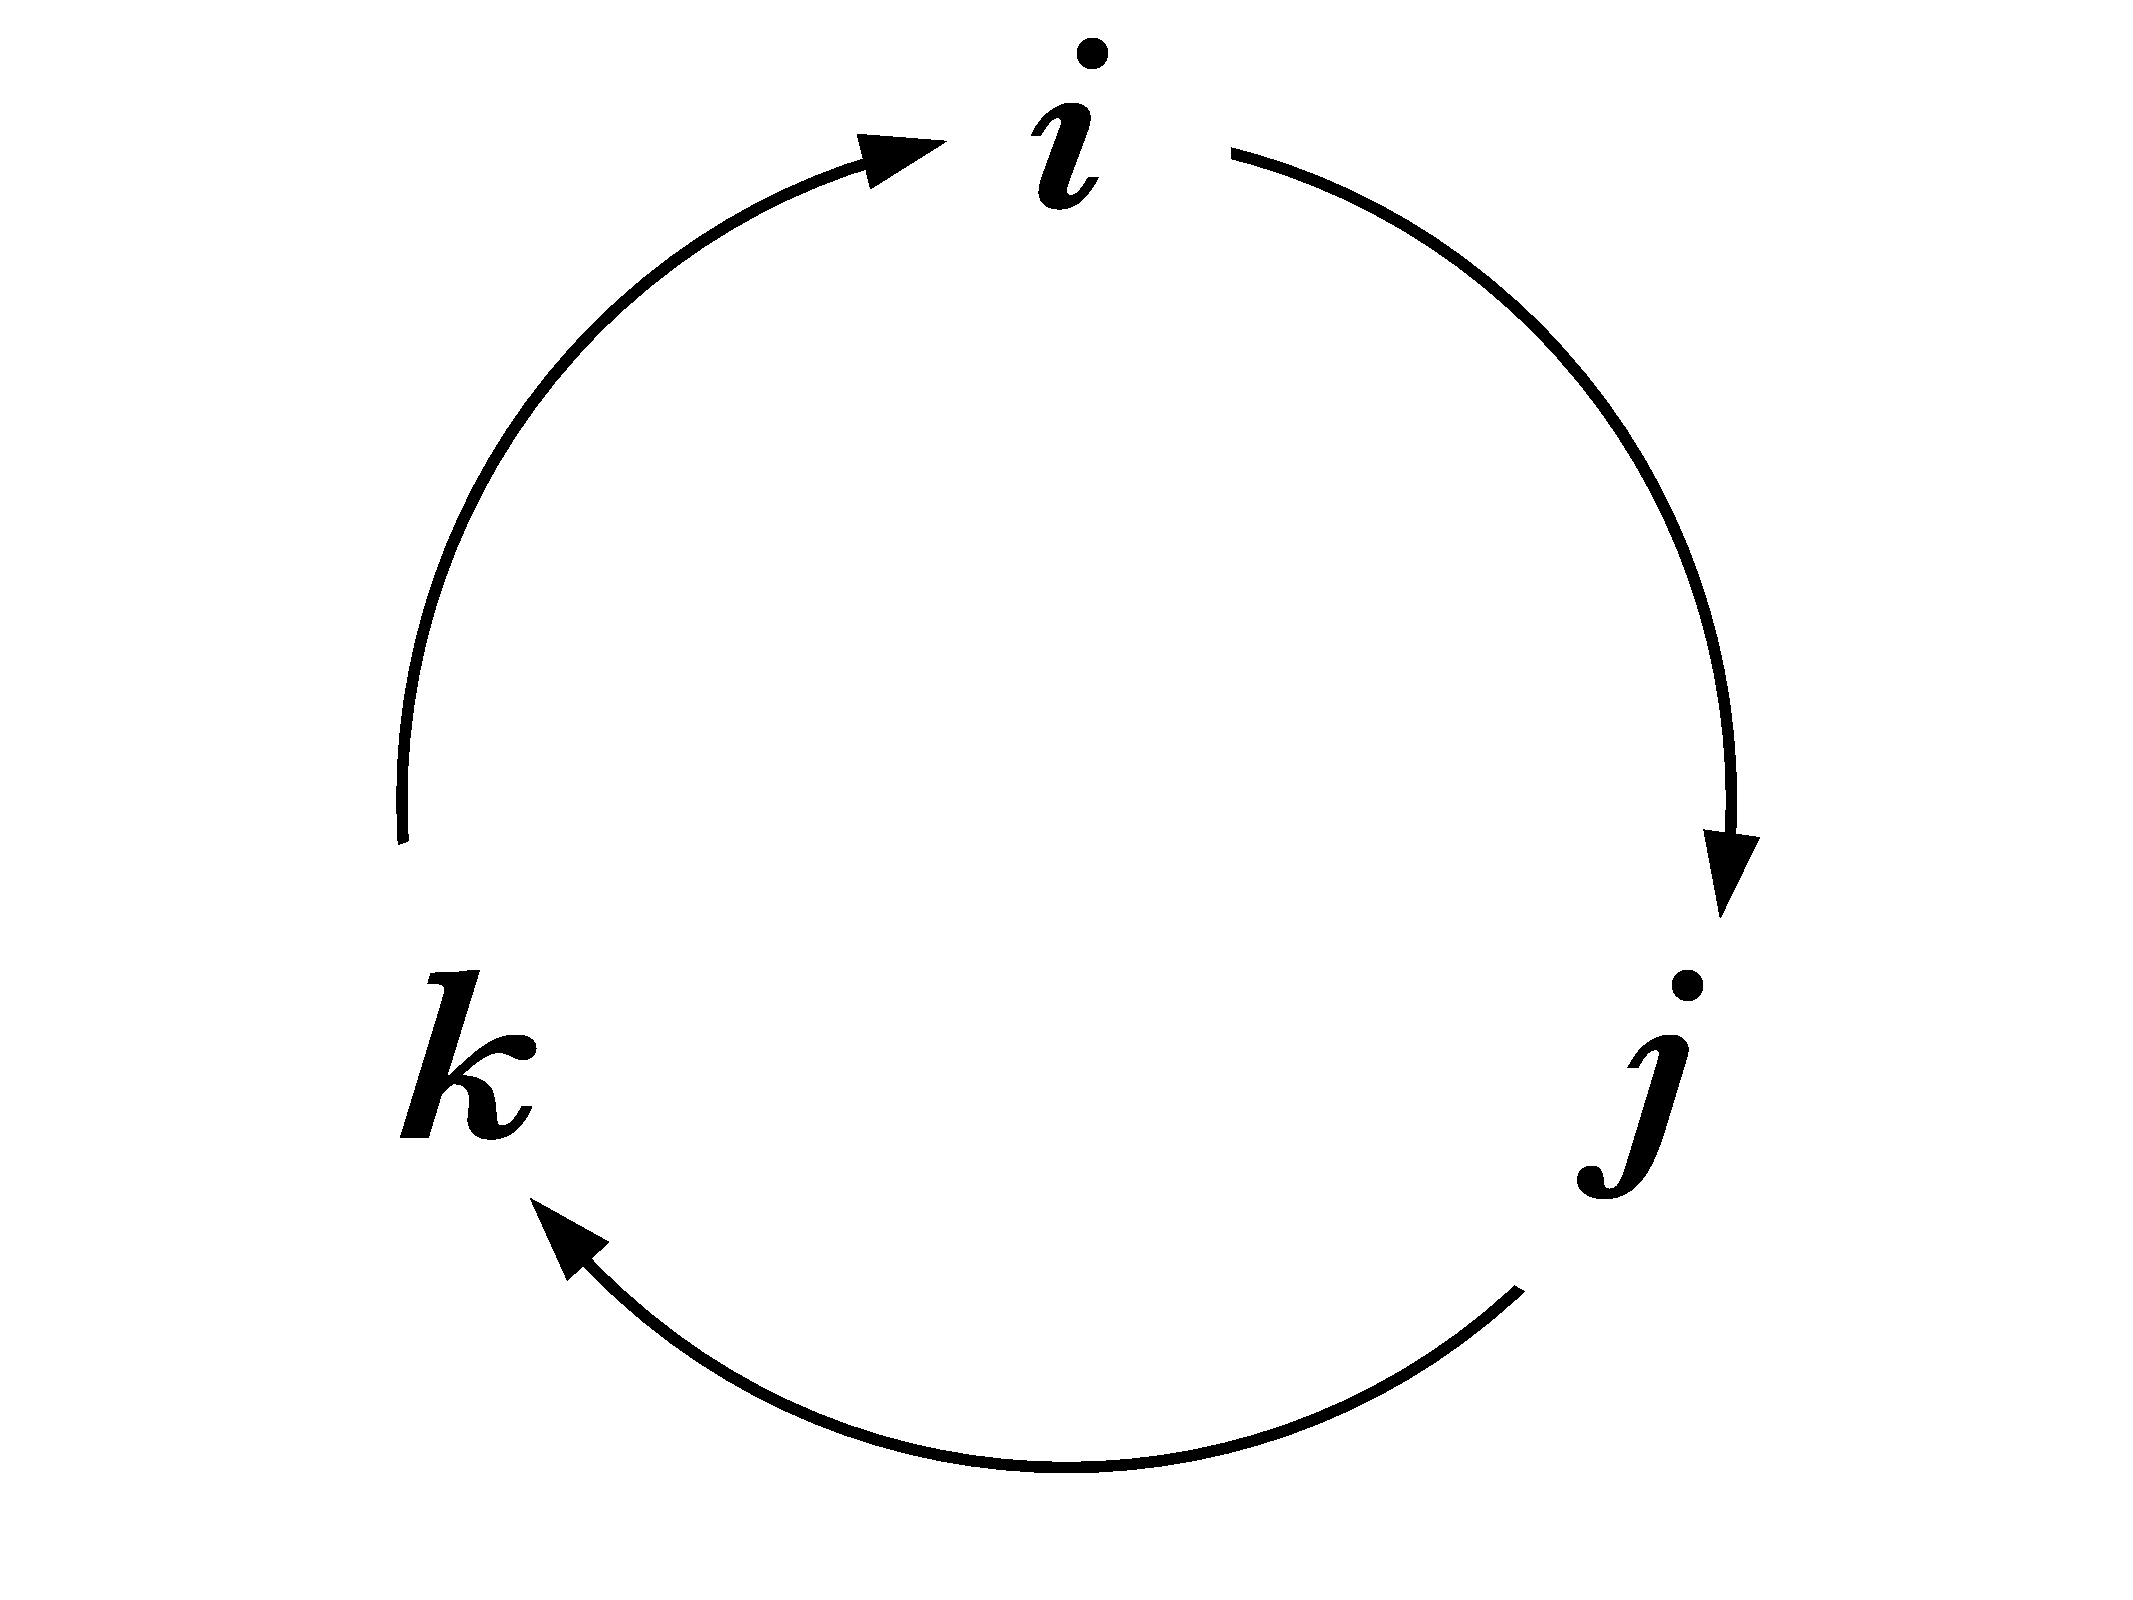
\includegraphics[width=0.2\linewidth]{Figures/quaternion_multiplication.pdf}
    \floatsource
    \label{fig:quatmult}
\end{figure}

The exploration of the quaternion multiplication rules gives rise to a useful property, related to products between complex numbers and elements from the quaternion canonical basis. In particular, the product between $\qj$ and any complex number $x = a + b \qi , \ a, b \in \mathbb{R}$, satisfies $\qj x = \overline{x} \qj$, since
\begin{equation}
    \label{eq:commutej}
    \begin{aligned}
        \qj x & = \qj (x_r + x_i \qi) = x_r \qj + x_i \qj \qi = x_r \qj - x_i \qi \qj \\
              & = (x_r - x_i \qi) \qj = \overline{x} \qj.
    \end{aligned}
\end{equation}
This will come up a couple of times during manipulations in this thesis.

The elements $\qi, \qj$ e $\qk$ may be perceived as orthogonal imaginary units, generating the 3D space of quaternion \textit{imaginary parts},
\begin{equation}
    \qV (q) = b\qi + c\qj + d\qk.
\end{equation}
The \emph{real part} of a quaternion \emph{q} is defined as
\begin{equation}
    S(q) = a.
\end{equation}

The imaginary part is usually referred to as \textit{vector part}, while the real part may also be called \textit{scalar part}. A quaternion with null real part is said to be \textit{pure} --- the set of which is represented by $\qV(\mathbb{H})$. The product between pure quaternions may be written similarly to that between $\mathbb{R}^3$ vectors, i.~e., if $v_1 = b_1\qi + c_1\qj + d_1\qk$ and $v_2 = b_2\qi + c_2\qj + d_2\qk$, then
\begin{equation}
    v_1 \times v_2 =
    \begin{vmatrix}
        \qi & \qj & \qk \\
        b_1 & c_1 & d_1 \\
        b_2 & c_2 & d_2
    \end{vmatrix}.
\end{equation}

Based on the similarity between the $ \mathbb{R}^3 $ set, equipped with the cross product, and the set of pure quaternions, equipped with their quaternion product, it is usual to refer to $\qi, \qj$ and $\qk$ as \emph{axis}. The term references the interpretation of theses imaginary units as being coordinate axis in the 3D space of pure quaternions.

The analogy with the $\mathbb{R}^3$ vector operations also extends to the definition of inner product between pure quaternions $v_1 = b_1\qi + c_1\qj + d_1\qk$ and $v_2 = b_2\qi + c_2\qj + d_2\qk$:
\begin{equation}
    \langle v_1, v_2 \rangle =
    b_1 b_2 + c_1 c_2 + d_1 d_2.
\end{equation}

The quaternion multiplication distributes over quaternion addition
% this english sentence is right: https://en.wikipedia.org/wiki/Distributive_property
and is also associative. That is, if $q_1 = a_1 + b_1\qi + c_1\qj + d_1\qk$ and $q_2 = a_2 +  b_2\qi + c_2\qj + d_2\qk$, then their sum is simply
\begin{equation}
    q_1 + q_2 = (a_1 + a_2) + (b_1 + b_2)\qi + (c_1 + c_2)\qj + (d_1 + d_2)\qk,
\end{equation}
whereas their product is
\begin{equation}
    \label{eq:q_prod}
    \begin{aligned}
        q_1 q_2 = & \ (a_1 + b_1\qi + c_1\qj + d_1\qk) (a_2 +  b_2\qi + c_2\qj + d_2\qk) \\
        =         & \ (a_1 a_2 - b_1 b_2 - c_1 c_2 - d_1 d_2)                            \\
                  & + \qi (b_1 a_2 + a_1 b_2 - d_1 c_2 + c_1 d_2)                        \\
                  & + \qj (c_1 a_2 + d_1 b_2 + a_1 c_2 - b_1 d_2)                        \\
                  & + \qk (d_1 a_2 - c_1 b_2 + b_1 c_2 + a_1 d_2).
    \end{aligned}
\end{equation}

Finally, it is possible to write the quaternion product in (\ref{eq:q_prod}) as a function of the operands scalar and vector parts,
\begin{equation}
    \label{eq:prod_vectors}
    \begin{aligned}
        q_1 q_2 = & \ S(q_1)S(q_2) - \langle\qV(q_1), \qV(q_2)\rangle              \\
                  & + S(q_1) \qV(q_2) + S(q_2)\qV(q_1) + \qV(q_1) \times \qV(q_2).
    \end{aligned}
\end{equation}
The lack of commutativity in the cross product is another demonstration of the fact that quaternion multiplication is noncommutative.

Quaternion conjugation, as defined in the complex numbers, is obtained changing the sign of the imaginary part: $ \bar{q} \overset{\Delta}{=} S(q) - \qV(q) $. The quaternion \textit{norm} is defined as $\Vert q \Vert \overset{\Delta}{=} a^2 + b^2 + c^2 + d^2 = q \bar{q} = \bar{q} q$, whereas the \textit{modulus} of $q$ \cite{ell2014quaternion} is
\begin{equation}
    \label{eq:modulusq}
    |q| \overset{\Delta}{=} \sqrt{a^2 + b^2 + c^2 + d^2} = \Vert q \Vert^{\nicefrac{1}{2}}.
\end{equation}

A closed expression for the product between the conjugate of two quaternions $q$ and $p$ may be obtained from (\ref{eq:prod_vectors}), by changing the sign in the vector part of the operands,
\begin{equation}
\bar{q} \bar{p} = S(q)S(p) - \langle\qV(q), \qV(p)\rangle
- S(q) \qV(p) - S(p)\qV(q) + \qV(q) \times \qV(p).
\end{equation}
Similarly, the conjugate of the product $pq$ may be taken simply by adding a minus sign in the vector part of the product $pq$, yielding
\begin{equation}
\overline{p q} = S(p)S(q) - \langle\qV(p), \qV(q)\rangle
- S(p) \qV(q) - S(q)\qV(p) - \qV(p) \times \qV(q).
\end{equation}
Since $\qV(p) \times \qV(q) = - \qV(q) \times \qV(p)$, it follows that $\bar{q} \bar{p} = \overline{p q}$. This result allows to prove that $\Vert p q \Vert = \Vert p \Vert \Vert q \Vert$, since
\begin{equation}
\label{eq:normproduct}
\begin{aligned}
    \Vert pq \Vert = \overline{pq} pq = \bar{q} \bar{p} p q = \bar{q} \Vert p \Vert q = \Vert p \Vert \bar{q} q =
    \Vert p \Vert \Vert q \Vert.
\end{aligned}
\end{equation}

A \textit{unit} quaternion has, by definition, unit norm, and the norm definition also leads to the quaternion multiplicative inverse (if $q \neq 0$),
\begin{equation}
    q^{-1} = \frac{\bar{q}}{\Vert q \Vert},
\end{equation}
from which follows that a quaternion and its multiplicative inverse have reciprocal moduli, i.~e.
\begin{equation}
    \label{eq:reciprocalmoduli}
    |q^{-1}| = \frac{|\bar{q}|}{\Vert q \Vert} =
    \frac{|q|}{|q|^2}=
    \frac{1}{|q|}.
\end{equation}

From the analogy between pure quaternions and the elements in $ \mathbb{R}^3 $, the idea of perpendicularity between pure quaternions presents itself naturally. Given $ \qmu,  \qnu \in \qV(\mathbb{H})$, they are said orthogonal --- we write $ \qmu \perp \qnu $ --- if and only if
\begin{equation}
    S(\qmu \qnu) = \langle \qmu, \qnu \rangle = 0.
    % \tag{$ \iff \qmu \perp \qnu $}
\end{equation}
For two orthogonal unit pure quaternions $ \qmu $ and $ \qnu $, it follows from (\ref{eq:prod_vectors}) that $ \qmu \qnu  = \qmu \times \qnu$, therefore $ \qmu \qnu \perp \qmu $ and $ \qmu \qnu \perp \qnu $. Since $ (\qmu, \qnu, \qmu \qnu) $ is a triplet of orthogonal unit pure quaternions, they form a basis for $ \qV (\mathbb{H}) $. Hence it is possible to rewrite (\ref{eq:q}) as
\begin{equation}
    \label{eq:quat_generalizado}
    q = a + b'\qmu + c'\qnu + d'\qmu \qnu,
\end{equation}
$a, b', c', d' \in \mathbb{R}$,
which represents the so called \emph{generalized quaternion}. The \emph{classical Hamiltonian quaternions} are those written in terms of the canonical basis $ (1, \qi, \qj, \qk) $.


Besides the cartesian representation (\ref{eq:q}), quaternions allow the so called \emph{Euler form} \cite{ell2014quaternion}, a polar representation commonly expressed as
\begin{equation}
    \label{eq:euler}
    q = |q| e^{\qmu \theta} = |q|\cos \theta + |q|\qmu \sen \theta,
\end{equation}
in which $ \qmu $ is a unit pure quaternion, parallel to the vector part of $ q $.

As a remarkable consequence of (\ref{eq:euler}), it follows that every unit pure quaternion is a square root of $-1$. For instance, let $ \qnu $ be a unit pure quaternion. From (\ref{eq:euler}),
\begin{equation}
    %\label{key}
    \qnu = |\qnu| e^{\qnu \theta},
\end{equation}
but since $ |\qnu| = 1 $, then
\begin{equation}
    %\label{key}
    \qnu = e^{\qnu \theta}  = \cos \theta + \qnu \sen \theta \Rightarrow \theta = \frac{\pi}{2},
\end{equation}
hence,
\begin{equation}
    %\label{key}
    \qnu^2 = \left( e^{ \qnu \frac{\pi}{2}} \right)^2 = e^{\qnu \pi} = \cos \pi + \qnu \sen \pi = -1.
\end{equation}

This property leads to the conclusion that numbers such as $ a + \qmu b  $ form an isomorphism with the complex numbers. For this reason, the set composed by such numbers is represented by $ \mathbb{C}_{\qmu} \overset{\Delta}{=} \{ a + \qmu b \ |\  a, b \in \mathbb{R} \}$ (and hence $ \mathbb{C}_{\qi} $ can be identified, for all practical ends, as the usual set of complex numbers, by making the extrapolation that the unit pure quaternion $\qi$ equals the complex imaginary unit).

Another crucial representation of quaternion numbers is called \emph{symplectic decomposition}. Every quaternion $ q = a + b\qi + c\qj + d\qk \in \mathbb{H} $ can be represented as
\begin{equation}
    q = q_1 + q_2 \qj, \quad q_1, q_2 \in \mathbb{C}_{\qi},
\end{equation}
in which the complex numbers $ q_1 = a + b\qi $ and $ q_2 = c + d\qi $ are commonly named \emph{simplex} and \emph{perplex} parts, respectively. In general, the decomposition does not need to take $\qi$ as reference axis. Take for example $ \qmu $ and $ \qnu $ as arbitrary orthogonal unit pure quaternions, hence any quaternion $ q $ may be decomposed as
\begin{equation}
    \label{eq:decomposicao}
    q = q_1 + q_2 \qnu, \quad q_1, q_2 \in \mathbb{C}_{\qmu}.
\end{equation}
That is a hugely important tool when it comes to computing the QDFT (see Section \ref{sec:QFT}) and handling quaternion matrices (cf. Chapter \ref{ch:QGSP}).

\subsection{Quaternion similarity and rotation}
\label{subsec:rotacionando}
Two quaternions $ q $ and $ r $ are said to be \emph{similar} if it exists a non-zero quaternion $ v $ such that $ v^{-1}q v = r $. In this case, one can write $ q \sim r $. Similarity between quaternions constitutes an equivalence relation \cite{zhang1997quaternions}, and all elements from a same similarity class possess the same norm, since, from (\ref{eq:normproduct}) and (\ref{eq:reciprocalmoduli}), $ |v^{-1}q v| = |v^{-1}| \cdot |q| \cdot |v| = |q| $.

It matters to notice that an important property of quaternion similarity transformations, which justifies its great use in mechanics and graphics computing industry, is that it performs a rotation on the $\qi \qj \qk$ space. Given $ v,q \in \mathbb{H} $, $ v = |v| e^{\qmu \alpha}$, the similarity transformation
\begin{equation}
    \label{eq:rotacao}
    \phi_v(q) = v q v^{-1}
\end{equation}
produces the rotation of the vector part of $q$ along the axis $ \qmu $ (which is parallel to the vector part of $v$) through an angle $ 2\alpha $ \cite{ward2012quaternions}, following the right-hand rule. Let us illustrate this property with an example.

\vspace{-2em}
\begin{quotation}
    \begin{example}
        \label{example:01}
        \upshape
        Let $ \lambda = 3\qi + \qk $ and
        \begin{equation}
            %\label{key}
            \mathbf{v} =\begin{pmatrix}
                1 +  \qi \\
                2 \qj + \qk
            \end{pmatrix}
        \end{equation}
        be, respectively, an eigenvalue and its eigenvector of a matrix $\mathbf{A} \in \mathbb{H}^{2 \times 2}$. The eigenvalue problem over the quaternions will be introduced in the next section, so let us not consider its details for now. It suffices to know that $\lambda$, $\mathbf{A}$ and $\mathbf{v}$ satisfy the equation
        \begin{equation}
            \label{eq:03}
            \mathbf{A} \mathbf{v} = \mathbf{v} \lambda.
        \end{equation}

        Let us restrict the first column of $\mathbf{A}$ to be equal to $ (1 \quad 1)^T $, so that the the matrix is now fully determined,
        \begin{equation}
            %\label{key}
            \mathbf{A} =
            \begin{pmatrix}
                1 & - \frac{1}{5} + \frac{3}{5} \qi + 2 \qj \\
                1 & -3 \qi + \qj
            \end{pmatrix}.
        \end{equation}

        Given an invertible quaternion $q$, the equation may be rewritten as
        \begin{equation}
            \label{eq:rewritten}
            \mathbf{A} (\mathbf{v} q) = (\mathbf{v} q) q^{-1} \lambda q,
        \end{equation}
        which presents the similarity transformation $q^{-1} \lambda q$. Since similar quaternions differ only by a rotation of their vector parts, it is clearly possible to find a quaternion $q$ so that the vector part of $q^{-1} \lambda q$ is parallel to $\qi$ --- that is, $q^{-1} \lambda q$ is a complex number. Let us go through that process.

        Since the vector part of $\lambda$ belongs to the $ \qi \qk $ plane, the idea is to use (\ref{eq:rotacao}) to rotate $\lambda$ along the $\qj$ axis (orthogonal to the rotation plane) by an angle of $ \theta = \tan^{-1} \frac{1}{3} $ radians, toward $ \qi $ (see Fig. \ref{fig:quat3ik}). The required quaternion to enable such rotation is, therefore,
        \begin{equation}
            \label{eq:04}
            v = e^{\qj \alpha}, \quad 2\alpha = \theta = \tan^{-1} \frac{1}{3},
        \end{equation}
        using the mapping $ \lambda \mapsto v \lambda v^{-1} $ in (\ref{eq:rotacao}).

        \begin{figure}
            \centering
            \caption{Representation of $ \lambda = 3\qi + \qk $ in the $ \qi \qk $ plane.}
            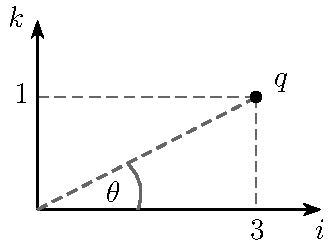
\includegraphics[width=0.3\linewidth]{Figures/quaternion01.pdf}
            \floatsource
            \label{fig:quat3ik}
        \end{figure}

        Recalling that our desired transformation is written as $ \lambda \mapsto q^{-1} \lambda q $, then
        \begin{equation}
            %\label{key}
            q = v^{-1} = e^{- \qj \alpha} = e^{- \qj \frac{\theta}{2}}.
        \end{equation}

        As a sanity check, let us find the value of $ \alpha $ which results in $ q^{-1} \lambda q \in \mathbb{C}_{\qi} $. Since $ v = q^{-1} = \cos \alpha + \qj \sin \alpha $,
        \begin{equation}
            %\label{key}
            \begin{aligned}
                %\label{key}
                q^{-1} \lambda   & = (\cos \alpha + \qj \sin \alpha)(3 \qi + \qk)                                                          \\
                                 & = \qi(3 \cos \alpha + \sin \alpha) + \qk(\cos \alpha - 3 \sin \alpha).                                  \\
                q^{-1} \lambda q & = [\qi(3 \cos \alpha + \sin \alpha) + \qk(\cos \alpha - 3 \sin \alpha)] (\cos \alpha - \qj \sin \alpha) \\
                                 & = \qi (3 \cos 2\alpha + \sin 2\alpha) + \qk(\cos 2\alpha - 3 \sin 2\alpha).
            \end{aligned}
        \end{equation}

        Therefore, $ q^{-1} \lambda q \in \mathbb{C}_{\qi} $ if and only if
        \begin{equation}
            %\label{key}
            \begin{aligned}\textbf{}
                \cos 2\alpha - 3 \sin 2\alpha & = 0                      \\
                \Rightarrow 2\alpha           & = \tan^{-1} \frac{1}{3},
            \end{aligned}
        \end{equation}
        as determined by (\ref{eq:04}).

        Consequently, it was demonstrated that the unit pure quaternion $ q = e^{- \qj \alpha} $, with $ \alpha = - \displaystyle \nicefrac{1}{2} \tan^{-1} \nicefrac{1}{3} $, produces, through a similarity transformation, the complex-valued eigenvalue $ q^{-1} \lambda q \in \mathbb{C}_{\qi}$. Since $q = \cos \alpha - \qj \sin \alpha $, (\ref{eq:03}) can be rewritten as in (\ref{eq:rewritten}),
        \begin{equation}
            %\label{key}
            \mathbf{A} \underbrace{\begin{pmatrix}
                    cos \alpha + \qi \sin \alpha - \qj \sin \alpha - \qk \sin \alpha \\
                    2 \sin \alpha + \qi \sin \alpha + \qj 2 \cos \alpha + \qk \cos \alpha
                \end{pmatrix}}_{= \mathbf{v} q} =
            (\mathbf{v} q) \cdot \underbrace{\qi (3 \cos 2\alpha + \sin 2\alpha)}_{= q^{-1} \lambda q}.
            %\underbrace{3.162 \qi}_{= \bar{u} q u}.
        \end{equation}
        Let us leave a remark for the user, as an anticipation of the upcoming section: notice how $\mathbf{v}$ and $\mathbf{v}q$ are the same eigenvector up to a scaling factor, and it is always possible to make $q^{-1} \lambda q$ into a complex number through a similarity transformation, given that the vector part of $\lambda$ has non-zero norm.
    \end{example}
\end{quotation}


\section{On the theory of quaternion matrices}

When analyzing the eigenstructure and subsequent fractionalization of the QDFT matrix, the eigendecomposition of the DFT and the eigenvector sharing served as a convenient shortcut. In order to build the results in QGSP, however, it is required to dive into more general properties of quaternion matrices. The symplectic decomposition, already presented in (\ref{eq:decomposicao}), plays an important role in that matter, especially for its use in defining the \textit{complex adjoint matrix}.

\begin{definition}[Complex adjoint matrix \cite{zhang1997quaternions}]
    \label{def:complexadjoint}
    Given $ \mathbf{A} \in \mathbb{H}^{n \times n} $, with symplectic decomposition $ \mathbf{A}_1 + \mathbf{A}_2 \qj$, $ \mathbf{A}_1,\mathbf{A}_2 \in \mathbb{C}^{n \times n} $, its complex adjoint matrix is defined as
    \begin{equation}
        \rchi_{A} \overset{\Delta}{=}
        \begin{pmatrix}
            \mathbf{A}_1              & \mathbf{A}_2            \\
            - \overline{\mathbf{A}}_2 & \overline{\mathbf{A}}_1
        \end{pmatrix}.
    \end{equation}
\end{definition}

In the following theorems, Zhang brings fundamental results for building QGSP.

\begin{theorem}[Part of Theorem 4.2 in
        \cite{zhang1997quaternions}
    ]
    \label{th:equiv01}
    Given the quaternion matrices $ \mathbf{A}, \mathbf{B} \in \mathbb{H}^{n \times n} $, the following sentences are equivalent:

    \begin{itemize}[noitemsep]
        \item $ \rchi_{AB} = \rchi_{A} \rchi_{B} $,
        \item $ \rchi_{A^{-1}} = \rchi_{A}^{-1}$, if $ \mathbf{A}^{-1} $ exists,
        \item $ \rchi_{A}$ is unitary, Hermitian or normal if and only if so is $ \mathbf{A} $.
    \end{itemize}

\end{theorem}

\begin{theorem}[Part of Theorem 4.3 in
        \cite{zhang1997quaternions}
    ]
    \label{th:equiv02}
    Given the matrix $ \mathbf{A} \in \mathbb{H}^{n \times n} $, the following sentences are equivalent:

    \begin{itemize}[noitemsep]
        \item $\mathbf{A}$ is invertible.
        \item $\mathrm{det}(\rchi_A) \neq 0$, i.~e., $\rchi_{A}$ is invertible.
    \end{itemize}

\end{theorem}

Differently from other representations of quaternion matrices in $ \mathbb{C} $ or $ \mathbb{R} $, the complex adjoint allows to establish an important relation between the spectra of $ \rchi_{A} $ and $ \mathbf{A} $, as will soon be discussed.

\subsection{Eigenvalues}
Since quaternion multiplication is noncommutative, it is necessary to distinguish between \textit{left} and \textit{right} eigenvalues of a given matrix $ \mathbf{A} \in \mathbb{H}^{n \times n} $,
\begin{align*}
    \mathbf{A} \mathbf{v} & = \mathbf{v} \lambda, \tag{right} \\
    \mathbf{A} \mathbf{v} & = \lambda \mathbf{v}.  \tag{left}
\end{align*}

We will restrict this discussion mostly to right eigenvalues, since they hold a broader set of results in literature \cite[Cap. 5]{zhang1997quaternions} and are, for that matter, a safer point of support when developing QGSP. When not explicitly mentioned, the right eigenvalues will simply be referred to as \textit{eigenvalues} of the quaternion matrix.

It matters to highlight the fact that a quaternion matrix possesses a \textit{finite} number of eigenvalues if and only if they are all real-valued. Otherwise, each of them will belong to a similarity class, according to the transformation $ \lambda_1 = q^{-1} \lambda_2 q $, containing \textit{infinite} quaternions which are also eigenvalues of the same matrix (return to Example \ref{example:01}, for instance). Let $ \lambda $ be an eigenvalue of the matrix $ \mathbf{A} $ associated with the eigenvector $ \mathbf{v} $. That is,
\begin{equation}
    \begin{aligned}
        \label{eq:similar}
        \mathbf{A} \mathbf{v}     & = \mathbf{v} \lambda                                   \\
        \mathbf{A} \mathbf{v} q   & = \mathbf{v} \lambda q = \mathbf{v} q q^{-1} \lambda q \\
        \mathbf{A} (\mathbf{v} q) & = (\mathbf{v} q) q^{-1} \lambda q,
    \end{aligned}
\end{equation}
so that $ q^{-1} \lambda q $ is an eigenvalue associated with the eigenvector $ \mathbf{v}q $, with $ q \in \mathbb{H}^\ast $.

\subsection{Diagonalizability}
\label{subsec:autovetores_XA}

The problem of quaternion matrix diagonalization differs greatly from the case with complex matrices. In the latter scenario, having no pair of equal eigenvalues is a sufficient condition for diaginalizability, but the rule does not hold for the quaternio case. See for instance the counterexample given by Zhang \cite[Exemplo 7.4]{zhang1997quaternions}, the matrix
\begin{equation}
    \mathbf{A} =
    \begin{pmatrix}
        \qi & 1   \\
        0   & \qj
    \end{pmatrix}.
\end{equation}

Although its eigenvalues are distinct -- $ \qi $ and $ \qj $, since they lie on the main diagonal of an upper triangular matrix --, the respective eigenvectors do not constitute a linearly independent set. Notice, for example, that an eigenvector associated with $ \qi $ is $ (1 \ 0)^T $, whereas one associated with $ \qj $ is $ (\qi + \qj \ 0)^T $. The reason as to why they form a linearly dependent set is the fact previously stated that, for each eigenvalue and eigenvector $ \lambda $ and $ \mathbf{v} $ from a quaternion matrix, it follows that $ q^{-1}\lambda q $ and $ \mathbf{v}q $ form another eigenvalue-eigenvector pair, with $ q \in \mathbb{H}^\ast $. That is, two \emph{similar} eigenvalues are always associated with the same eigenvector (up to a scaling factor). That is why similar quaternions are said to belong to the same \emph{eigenclass} \cite{de2000right}. In order to have a linearly independent set of eigenvectors, therefore, their eigenvalues must not be similar. Concluding the counterexample, the reader may show that $ \qi $ and $ \qj $ satisfy the similarity relation $ \qj = q \qi q^{-1} $ whenever $q$ belongs to the set $ \{ a - a\qi - a\qj + a\qk \ | \ a\in \mathbb{R}^\ast \} $.

Theorem \ref{th:02} relates the eigendecomposition of a quaternion matrix to that of its complex adjoint, providing a fundamental principle to the study of quaternions matrices' eigenstructure.

\begin{figure}
    \centering
    \caption{\emph{Standard eigenvalues} of a quaternion matrix $ \mathbf{A} $, indicated as a subset of the eigenvalues of the complex adjoint matrix.}
    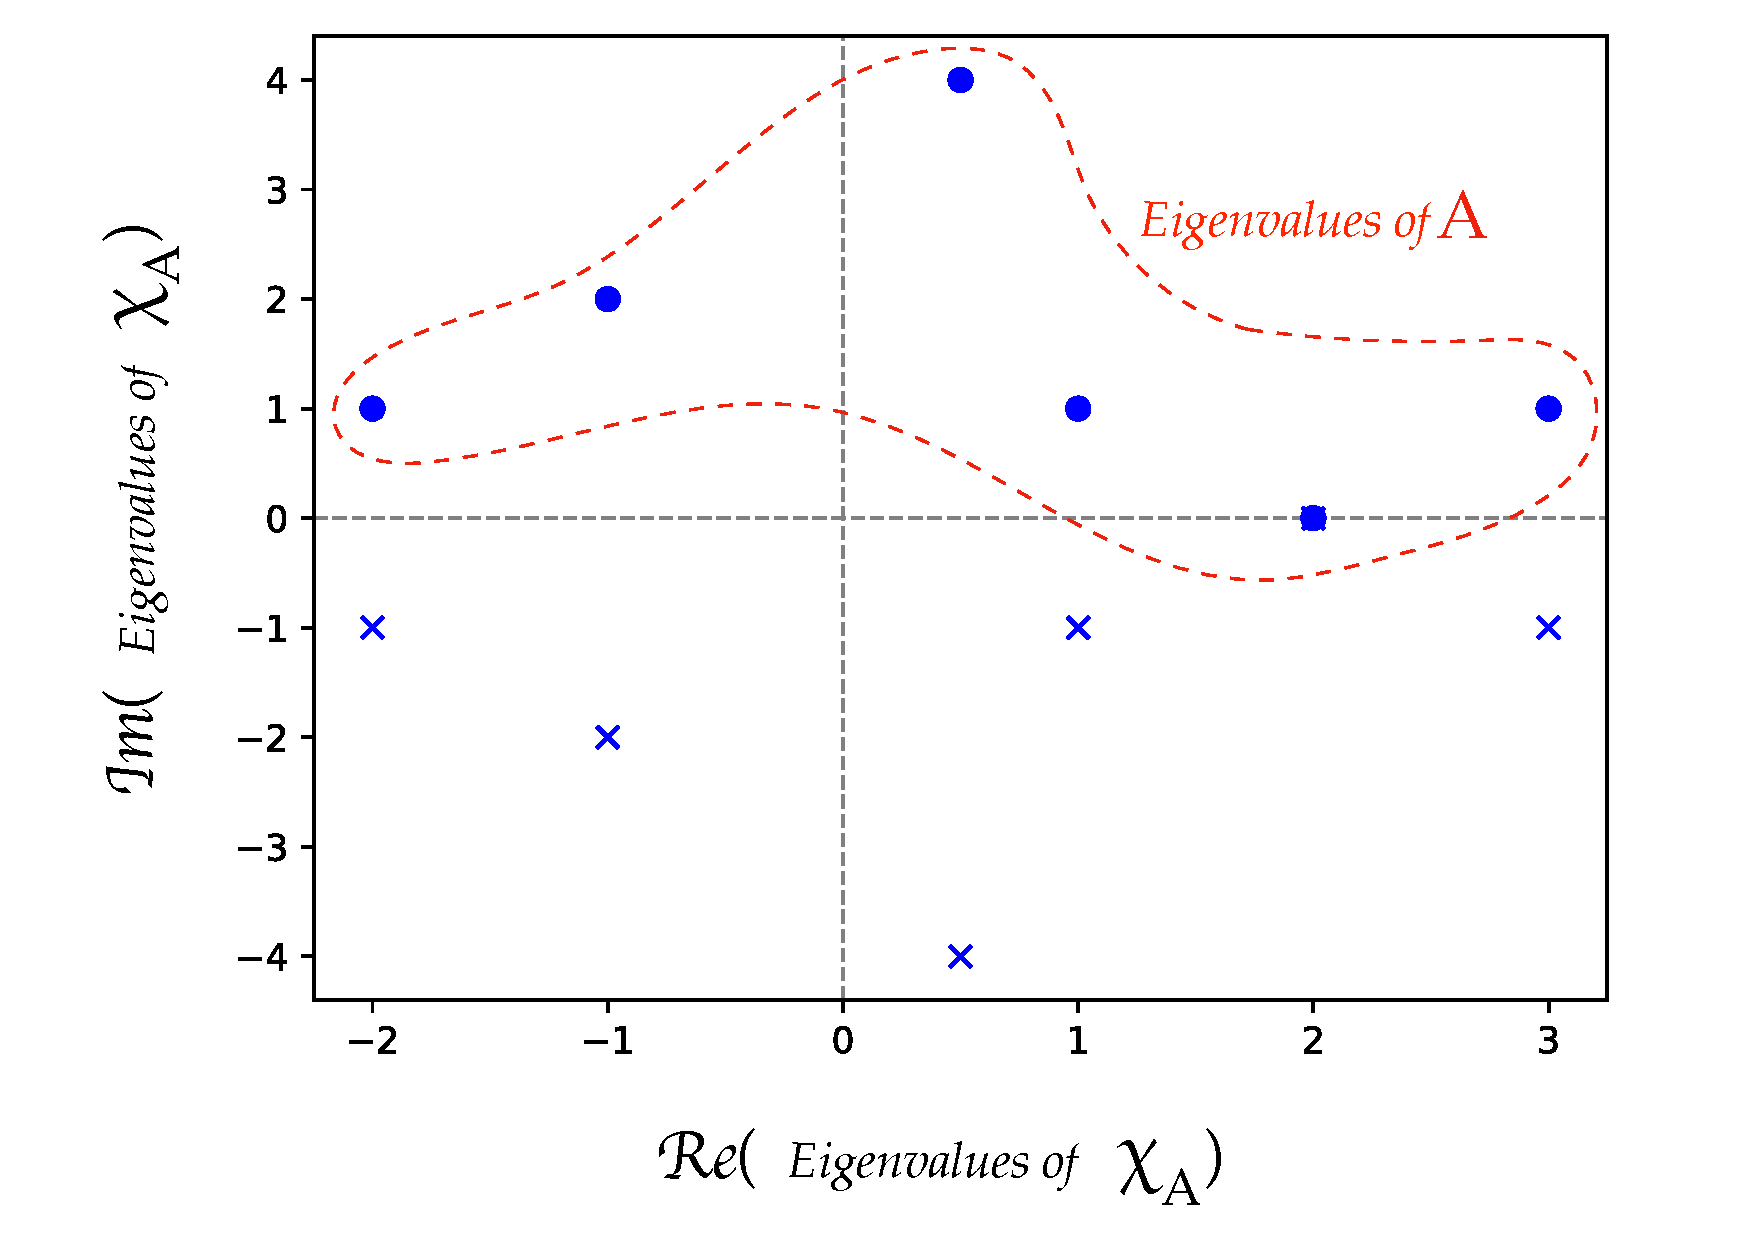
\includegraphics[width=0.7\linewidth]{Figures/complex_adjoint_eigvals_EN.pdf}
    \floatsource
\end{figure}


\begin{theorem}[\cite{zhang1997quaternions}]
    \label{th:02}
    Every matrix $ A \in \mathbb{H}^{n \times n} $ has exactly $ n $ right eigenvalues which are complex numbers with nonnegative imaginary parts. These are called the \textbf{standard eigenvalues} of $ \mathbf{A} $ and are a subset of the $ 2n $ eigenvalues of $ \rchi_A $.
\end{theorem}

\begin{proof}
    As demonstrated in the Appendix \ref{ch:AppendixA}, starting from the quaternion eigenvalue equation
    \begin{equation}
        \mathbf{A} \mathbf{v} = \mathbf{v} \lambda,
    \end{equation}
    in which one can assume without loss of generality that $ \lambda \in \mathbb{C} $, it is always possible to arrive at the \emph{equivalent} equation
    \begin{equation}
        \label{eq:eigvalueequation}
        \begin{pmatrix}
            \mathbf{A}_1              & \mathbf{A}_2            \\
            - \overline{\mathbf{A}}_2 & \overline{\mathbf{A}}_1
        \end{pmatrix}
        \begin{pmatrix}
            \mathbf{v}_1 \\
            - \overline{\mathbf{v}}_2
        \end{pmatrix} =
        \begin{pmatrix}
            \mathbf{v}_1 \\
            - \overline{\mathbf{v}}_2
        \end{pmatrix}
        \lambda,
    \end{equation}
    which involves solely complex-valued matrices and vectors, namely: the components of the symplectic decomposition of $ \mathbf{A} $ and $ \mathbf{v} $. The equivalence between both equations implies that $\mathbf{A}$ and its complex adjoint
    \begin{equation}
        \rchi_A =
        \begin{pmatrix}
            \mathbf{A}_1              & \mathbf{A}_2            \\
            - \overline{\mathbf{A}}_2 & \overline{\mathbf{A}}_1
        \end{pmatrix}
    \end{equation}
    \textit{share all their complex-valued eigenvalues} (notice that $\lambda$ remains unchanged as we move from one equation to its equivalent). As it appears, the eigendecomposition of the complex adjoint seems a promising method for finding some eigenvalues of the quaternion matrix.

    Is there, however, any possibility of leaving some eigenvalues behind? In other words, is it possible to exist some eigenvalue of $\mathbf{A}$ which does not belong to an eigenclass determined by a complex eigenvalue of $\rchi_A$? No, it is not, because it is always possible to align a quaternion's vector part with the $\qi$ axis through a single rotation (see Section \ref{subsec:rotacionando}). In other words,
    %all quaternions are similar to a specific complex number and, therefore,
    all (quaternion-valued) eigenvalues of $\mathbf{A}$ are similar to a complex number which, as discussed, must also be an eigenvalue of $\rchi_A$.

    Since $\rchi_A$ is a $ 2n \times 2n $-complex matrix, it has $ 2n $ complex-valued eigenvalues (possibly repeated). The reason why $\rchi_A$ share $2n$ eigenvalues with $\mathbf{A}$, even though $\mathbf{A}$ is an $ n \times n $ matrix is, once more, due to the existance of eigenclasses.

    According to \cite[Theorem 5]{lee1948eigenvalues}, the complex adjoint eigenvalues appear as $ n $ conjugate pairs (possibly some pairs are real-valued, so they are actually identical). Let us say that $2m$ of those eigenvalues are real, leaving $2(n-m)$ complex eigenvalues. Let $ q \in \mathbb{C}_{\qi}$ belong to the latter group. It can be shown imediately that $ q \sim \overline{q} $, since $ \overline{q} $ is obtained through a 180$ ^\circ $ rotation of the vector part of $ q $ around the $ \qj $ axis. This similarity transformation was already shown in (\ref{eq:commutej}), written as $\qj x = \overline{x} \qj$, or equivalently $\qj x (-\qj)= \overline{x}$. In the format of (\ref{eq:rotacao}), $ q \mapsto v q v^{-1} = \overline{q}$ with $ v = e^{\qj \frac{\pi}{2}} = \qj $.

    % (and so $ v^{-1} = e^{- \qj \frac{\pi}{2}} = -\qj $) to perform the simlarity transformation $ q \mapsto v q v^{-1} $,
    % \begin{equation}
    % \begin{aligned}
    % v q v^{-1} &= \qj (q_r + q_i \qi) (-\qj) = q_r - q_i \qj \qi \qj\\
    % &= q_r + q_i \qi \qj \qj = q_r - q_i \qi = \overline{q}.
    % \end{aligned}
    % \end{equation}
    Since two conjugate eigenvalues of $ \rchi_A $ are always similar, they belong to the same eigenclass and are therefore associated with the same set of linearly dependent eigenvectors. For that reason, by convention one can take the eigenvalues of $ \rchi_A $ and define the standard eigenvalues of $\mathbf{A}$ as being those complex-valued eigenvalues with positive imaginary part and half those real-valued ones.
\end{proof}

The following theorem is another fundamental result relating the eigenstructure of a quaternions matrix and that of its complex adjoint.

\begin{theorem}[Theorem 7.4 in \cite{zhang1997quaternions}]
    \label{th:diagonal}
    Given the matrices $ \mathbf{A}, \mathbf{B} \in \mathbb{H}^{n \times n} $, then $ \mathbf{A} $ is similar to $ \mathbf{B} $ if and only if $ \rchi_A $ is similar to $ \rchi_B $.
\end{theorem}

\begin{corollary}
    \label{cor:diagonalizable}
    A matrix $  \mathbf{A} \in \mathbb{H}^{n \times n} $ is diagonalizable if and only if $ \rchi_A $ is diagonalizable.
\end{corollary}
\begin{proof}
    If $ \mathbf{A} \in \mathbb{H}^{n \times n} $ is diagonalizable, then it is similar to a diagonal matrix $ \Lambda \in \mathbb{C}^{n \times n}_{\qi} $ containing its standard eigenvalues in the main diagonal. From Theorem \ref{th:diagonal}, it follows that $ \rchi_A $ is similar to
    \begin{equation}
        \label{eq:Xlambda}
        \rchi_{\Lambda} =
        \begin{pmatrix}
            \Lambda    & \mathbf{0}         \\
            \mathbf{0} & \overline{\Lambda}
        \end{pmatrix},
    \end{equation}
    which is also a diagonal matrix. Therefore, $ \rchi_A $ is diagonalizable.

    On the other hand, if $ \rchi_A $ is diagonalizable, then it is similar to a diagonal matrix containing its $ 2n $ eigenvalues, which appear in $ n $ conjugate complex pairs. Therefore, its eigenvalues matrix may be written as (\ref{eq:Xlambda}), what implies, from Theorem \ref{th:diagonal}, that $ \mathbf{A} $ is similar to $ \Lambda $.
\end{proof}

\section{The quaternion Fourier transform}
\label{sec:QFT}
The field of quaternion signal processing has leveraged many tools to transform signals with quaternion-valued samples, from the fundamental redefinition of the gradient operador \cite{jiang2014general} up to algorithms for adaptive filtering \cite{jiang2013frequency}. This section focuses on the quaternion Fourier transform (QFT), as it is the basis for spectral analysis of quaternion signals.

Quaternion Fourier transforms have received quite a few definitions. Some are one-dimensional \cite{flamant2017spectral}, while others are intrinsically two-dimensional \cite{guanlei2008fractional}; the latter group can yet be divided into those having kernels oriented toward generic unit pure quaternions, and those using canonic imaginary units, such as $ \qi $ and $ \qj $. The 2D-transformed signals may be placed \textit{between} the two kernels or beside them. In fact, Ell \cite[sec. 3.2]{ell2014quaternion} lists 8 possibilities for the 2D-QFTs. The two dimensional case will not be covered for now, since the discussion on the 1D case already serves the purpose of introducing the main ideas and properties of this family of transforms.

Let $f$ be a quaternion-valued function $f: \mathbb{R} \rightarrow \mathbb{H}$ and $\qmu \in \qV(\mathbb{H})$, $\qmu^2 = -1$. The \textit{left} 1D QFT can be defined as the family of integral transforms
\begin{equation}
    \mathcal{F}^L_{\mp \qmu}[f](\omega) =
    F^L_{\mp \qmu}(\omega) \overset{def}{=}
    \kappa_{-} \int_{-\infty}^{\infty} e^{\mp \qmu \omega t} f(t) \mathrm{d}t.
    \tag{left 1D QFT}
\end{equation}

It can be proven that the inverse transform exists and is given by
\begin{equation}
    \mathcal{F}^{-L}_{\pm \qmu}[F^L](t) =
    f(t) =
    \kappa_{+} \int_{-\infty}^{\infty} e^{\pm \qmu \omega t} F^L(\omega) \mathrm{d}\omega.
    \tag{inverse left 1D QFT}
\end{equation}

In the expressions above, the unit pure quaternion $\qmu$ is called the \emph{eigenaxis} of the transform kernel. We could say it is the reference imaginary unit. The sign in the exponential is arbitrary, as long as the direct and inverse transforms use different signs. The real constants $\kappa_{-}$ and $\kappa_{+}$ satisfy
\begin{equation}
    \kappa_{+} \kappa_{-} = \frac{1}{2\pi},
\end{equation}
\noindent and when $\kappa_{-} = \kappa_{+}$, the transform is said to be unitary.

The right QFT may be defined likewise, by simply switching the relative positions of the kernel and the operand $f(t)$. The reader may notice that, when the eigenaxis is $\qi$, the QFT coincides with the usual continuous-time Fourier transform.

In this work, however, the most relevant version of the QFT is that in which both the original signal and its transformed representation are defined over discrete domains: the 1D quaternion discrete Fourier Transform (QDFT) with axis $ \qmu $, as defined in \cite[sec. 3.3.1]{ell2014quaternion}. If $ \qmu $ is a unit pure quaternion, the $ m $-th component of the transformed vector in the left unitary QDFT with axis $ \qmu $ is
\begin{equation}
    \label{eq:QDFT_fwd}
    \widehat{v}_m = \text{QDFT}\{ \mathbf{v} \}_m \overset{\Delta}{=} \frac{1}{\sqrt{N}} \sum_{n=0}^{N-1}  \exp \left( -\qmu \frac{2\pi}{N} nm \right) v_n \in \mathbb{C}_{\qmu},
\end{equation}
with inverse transform given by
\begin{equation}
    \label{eq:QDFT_inv}
    v_n = \text{QDFT}^{-1}\{ \widehat{\mathbf{v}} \}_n = \frac{1}{\sqrt{N}}\sum_{m=0}^{N-1}  \exp \left( \qmu \frac{2\pi}{N} nm \right) \widehat{v}_m.
\end{equation}

The transform analysis and synthesis equations may also be written in matrix form:
\begin{equation}
    \label{eq:QDFT}
    \widehat{\mathbf{v}} = \text{QDFT}\{ \mathbf{v} \} = \mathbf{F} \mathbf{v},
\end{equation}
\begin{equation}
    \label{eq:QDFT_mtx_inv}
    \mathbf{v} = \text{QDFT}^{-1}\{ \widehat{\mathbf{v}} \} = \mathbf{F}^{-1} \widehat{\mathbf{v}},
\end{equation}
in which $ \mathbf{F} $ is the unitary transform matrix,
%--multiplicando sempre \`a esquerda--,
with entries $ \{\mathbf{F}\}_{n,m} = \sqrt{N}^{-1} \exp \left( -\qmu \frac{2\pi}{N} nm \right)$. Since  $ \exp \left( -\qmu \frac{2\pi}{N} \right) $ is a $ N $-th root of unity, just like $ \exp \left( -\qi \frac{2\pi}{N} \right) $, it follows that $ \mathbf{F} $ shares many properties with the usual discrete Fourier transform (DFT) matrix, among which the invertibility, validating the existence of (\ref{eq:QDFT_inv}) and (\ref{eq:QDFT_mtx_inv}).

As it was done in previous pages, the symplectic decomposition may be applied to each entry of a quaternion matrix, generating complex-valued \emph{simplex} and \emph{perplex} matrices.\footnote{Please note that, in what follows, the usual subscripts $1$ and $2$ for denoting the simplex and perplex parts were replaced by the superscripts $^{(s)}$ and $^{(p)}$, as in $q = q^{(s)} + q^{(p)} \qj$, to avoid confusion with the summation indices.} Using this reasoning, Ell e Sangwine \cite{ell2014quaternion} demonstrated that the QDFT of a signal $ \mathbf{x} = [x_0, x_1, \dots, x_{N-1}] \in \mathbb{H}^N $ could be easily computed using two (complex) DFT, by decomposing each signal sample along the QDFT eigenaxis:
%. Relembrando a eq. (\ref{eq:QDFT_fwd}),
\begin{equation}
    \begin{aligned}
        %\label{eq:QDFT_fwd}
        \text{QDFT}\{ \mathbf{x} \}_m & = \frac{1}{\sqrt{N}} \sum_{n=0}^{N-1} \exp \left( -\qmu \frac{2\pi}{N} nm \right) x_n                         \\
                                      & = \frac{1}{\sqrt{N}} \sum_{n=0}^{N-1} \exp \left( -\qmu \frac{2\pi}{N} nm \right) (x_n^{(s)} + x_n^{(p)}\qnu) \\
                                      & = \text{DFT}_{\qmu}\{ \mathbf{x}^{(s)} \}_m +
        \text{DFT}_{\qmu}\{ \mathbf{x}^{(p)} \}_m \qnu,
    \end{aligned}
\end{equation}
in which $ \text{DFT}_{\qmu} $ indicates the DFT computed with ``complex numbers'' having $ \qmu $ as imaginary unit.
Although that statement is technicaly incorrect (complex numbers strictly belong to $\mathbb{C}_{\qi}$), from a computational point of view, the $ \text{DFT}_{\qmu} $ can be calculated using the very same algorithms as the usual DFT (since the imaginary unit \textit{per se} is disregarded in the low-level calculations).

This brief presentation of the QDFT illustrates that
\begin{itemize}[noitemsep]
    \item although the frequency components are quaternion signals, their frequencies are real-valued (see the argument in the transform kernel),
    \item the eigenstructure of the QDFT likens heavily that of the usual DFT, to the point of allowing the reuse of common DFT algorithms. This resemblance will be exploited when investigating the fractionalization of the QDFT, in Chapter \ref{ch:FrQDFT}.
\end{itemize}

For a thorough introduction on quaternions and their application to signal processing, the reader may refer to \cite{grigoryan2018quaternion,zhang1997quaternions,ell2014quaternion,flamant2017time, jiang2014general}.

\section{Summary}

This chapter discussed the main topics concerning the quaternion algebra and its Fourier transform. Although they have not been addressed with the depth and details a more curious reader would wish, the discussion was hopefully enough to present a coherent overview of
\begin{itemize}[noitemsep]
    \item how the quaternions extend the complex numbers, by carrying not 2 but 4 real-valued components splitted into a scalar and a vector part,
    \item how the quaternion multiplication rules effect the quaternion similarity classes, with their rotation property,
    \item how the symplectic decomposition and the complex adjoint matrices are core concepts in the eigendecomposition of a quaternion matrix, and
    \item how to compute the left 1D discrete quaternion Fourier transform by using usual DFT calculations.
\end{itemize}
\chapter{A review on fractional and graph Fourier transforms}
\label{ch:reviewGSP}

At the heart of the field of spectral analysis lies the concept of \textit{Fourier transforms}, all of which are creatively tailored to map the original signal onto convenient new spaces. This links directly to the argument presented in the Introduction of this thesis: the power and flexibility of signal processing stem from the many ways in which one can explore different signal representations. While the last chapter ended with a brief presentation of the QFT, the next pages will guide the reader through an overview on two sets of transforms which are also relevant to understanding the contributions in the thesis: the fractional Fourier transform (FrFT) and the graph Fourier transform, the latter included in the broader discussion on fundamentals of graph signal processing.

\section{The fractional Fourier transform}

It is quite common in theoretical investigations to expand the definition of some well-established operator and consider the consequences of an intermediate (fractional) application of the underlying operation. Take, for example, the power operation, which makes \textit{sense} only for integer exponents (i.~e., $x^3 \overset{\Delta}{=} x \cdot x \cdot x$), but has great use when considering also real or complex exponents. Or the derivative of a function $f(t)$, which can be defined to possess a fractional-order equivalent by setting $n$ to non-integer values in the time differentiation property of the Fourier transform $\mathcal{F} \left\{ \cdot \right\}$:
\begin{equation}
\label{eq:derivative}
\mathcal{F} \left\{ \left[ \frac{\mathrm{d}^n}{(\mathrm{d}t)^n} f(t) \right] \right\} =
(\qj \omega)^n \mathcal{F} \left\{ f(t) \right\}.
\end{equation}
Mendlovic and Ozaktas made this observation \cite{mendlovic1993fractionalI} and pointed out that this was the spark behind the creation of the FrFT. However theoretical this endeavor might have been, even at its origin in the 1980's paper on the Journal of Applied Mathematics by the physicist Victor Namias \cite{namias1980fractional}, the fractional Fourier transform had already potential applications, originally in quantum mechanics. After 40 years, the FrFT has been applied to time-frequency analysis, compression, digital watermarking, filtering, encryption, let alone its utility in Optics \cite{bultheel2002shattered,figueiredo2018}.

The fractional Fourier transform is a generalization of the usual continuous-time Fourier transform and can be interpreted as a rotation of the signal (operand) in the time-frequency plane \cite{almeida1994fractional}. To understand why, let us consider its definition. The usual (unitary) Fourier transform, with operator represented by $\mathcal{F}$ as in (\ref{eq:derivative}), has analysis and synthesis equations given by
\begin{equation}
\mathcal{F}\left\{ f(t) \right\} = F(\qi \omega) = \frac{1}{\sqrt{2 \pi}} \int_{-\infty}^{\infty} f(t) \exp(-\qi \omega t) \mathrm{d}t,
\end{equation}
\begin{equation}
\mathcal{F}^{-1}\left\{ F(\qi \omega) \right\} = f(t) = \frac{1}{\sqrt{2 \pi}} \int_{-\infty}^{\infty} F(\qi \omega) \exp(\qi \omega t) \mathrm{d}\omega.
\end{equation}

The eigenfunctions of the $\mathcal{F}$ operator are the family of functions $\exp (\frac{-x^2}{2}) H_n(x)$ (on the variable $x$), where $H_n(x)$ are the Hermite polynomials of order $n$ \cite{namias1980fractional}. The associated eigenvalues have the form $\exp(- \qj n \frac{\pi}{2})$; therefore, if we add the notation $\mathcal{F}_{\frac{\pi}{2}} \overset{\Delta}{=} \mathcal{F}$,
\begin{equation}
\label{eq:eighermite}
\mathcal{F}_{\frac{\pi}{2}} \left\{ \exp \left(\frac{-x^2}{2}\right) H_n(x) \right\} = 
\exp\left(- \qj n \frac{\pi}{2}\right)
\exp \left(\frac{-x^2}{2}\right) H_n(x).
\end{equation}

The FrFT is then \textit{defined} as the operator $\mathcal{F}_\alpha$ satisfying the eigenvalue equation
\begin{equation}
\label{eq:frftdef}
\mathcal{F}_{\alpha} \left\{ \exp \left(\frac{-x^2}{2}\right) H_n(x) \right\} = 
\exp\left(- \qj n \alpha\right)
\exp \left(\frac{-x^2}{2}\right) H_n(x),
\end{equation}
from which follows that $\alpha = 0$ yields the identity operator and $\alpha = \frac{\pi}{2}$ makes the FrFT coincide with the usual Fourier transform (by definition). The \textit{order} of the fractional Fourier transform is defined by $m = \frac{2\alpha}{\pi}$.

The integral form of the operator $\mathcal{F}_\alpha$ is
\begin{equation}
\label{eq:integralfrft}
\mathcal{F}_\alpha \left\{ f(t) \right\} = \int_{-\infty}^{\infty} f(t) K_\alpha (t, u) \mathrm{d}t,
\end{equation}
in which the transformation kernel $K_\alpha (t, u)$ is given by
\begin{equation}
K_\alpha (t, u) = 
\begin{cases}
\sqrt{\frac{1 - \qj \cot \alpha}{2\pi}} \exp \left( \qj \frac{t^2 + u^2}{2} \cot \alpha - \qj ut \csc \alpha\right), &
\text{if $\alpha$ is not a multiple of $\pi$,} \\
\delta (t - u), & \text{if $\alpha$ is a multiple of $2\pi$,} \\
\delta (t + u), & \text{if $\alpha + \pi$ is a multiple of $2\pi$.}
\end{cases}
\end{equation}

\begin{figure}
\centering
\caption{Illustration of the FrFT property of rotation in the time-frequency plane.}
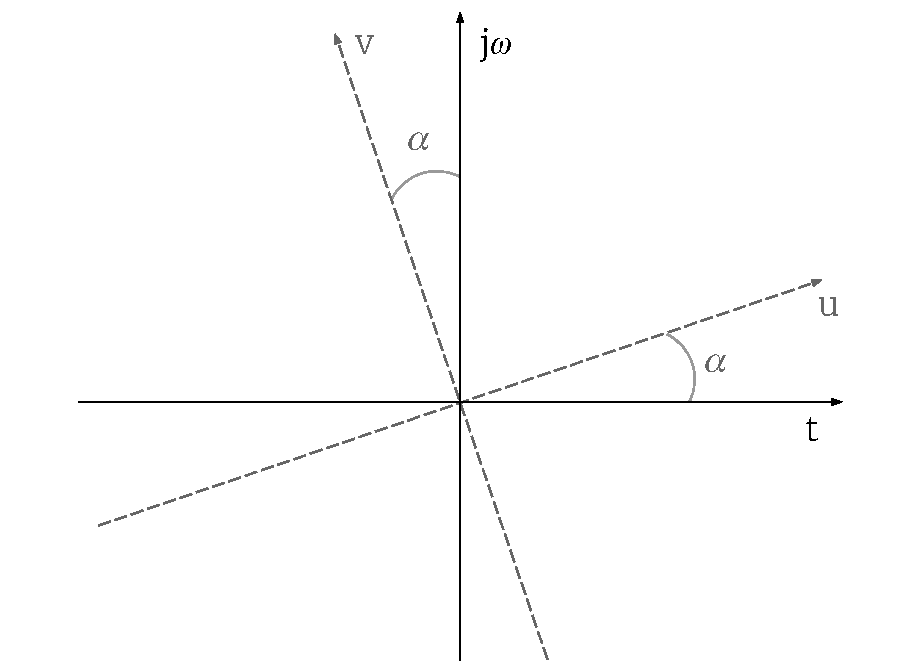
\includegraphics[width=0.65\linewidth]{Figures/FrFT-Rotation-cropped.pdf}
\floatsource[adapted from \cite{almeida1994fractional}]
\label{fig:frft_rotation}
\end{figure}

Two successive applications on the signal $f(t)$ of the FrFT with orders $m_1 = \frac{2\alpha_1}{\pi}$ and $m_2 = \frac{2\alpha_2}{\pi}$ can be written in a single equation as
\begin{align}
\label{eq:frftsucessive}
\mathcal{F}_{\alpha_2} \left\{ \mathcal{F}_{\alpha_1} \left\{ f(t) \right\} \right\} &=
\int_{-\infty}^{\infty} 
\left( \int_{-\infty}^{\infty} f(t) K_{\alpha_1} (t, s) \mathrm{d}t \right)
K_{\alpha_2} (s, u) \mathrm{d}s \\
&= 
\int_{-\infty}^{\infty}
f(t)
\left(
\int_{-\infty}^{\infty}
K_{\alpha_1} (t, s) K_{\alpha_2} (s, u) \mathrm{d}s
\right)
\mathrm{d}t.
\end{align}
After a ``rather long derivation'', according to \cite{almeida1994fractional}, it has been shown that
\begin{equation}
\label{eq:summingangles}
\int_{-\infty}^{\infty}
K_{\alpha_1} (t, s) K_{\alpha_2} (s, u) \mathrm{d}s = 
K_{\alpha_1 + \alpha_2} (t, u),
\end{equation}
and this implies
\begin{align}
\mathcal{F}_{\alpha_2} \left\{ \mathcal{F}_{\alpha_1} \left\{ f(t) \right\} \right\} &=
\int_{-\infty}^{\infty}
f(t)
K_{\alpha_1 + \alpha_2} (t, u)
\mathrm{d}t
= \mathcal{F}_{\alpha_1 + \alpha_2} \left\{ f(t) \right\}.
\end{align}
In other words, the FrFT has the property of additivity of transform orders. Let us see how this fits quite nicely with the known behavior of successive applications of the usual unitary Fourier transform.

It is known that Fourier-transforming twice the same signal yields the operand with reflected time axis,
\begin{equation}
\mathcal{F}^{(2)} \left\{ f(t) \right\} \overset{\Delta}{=}
\mathcal{F} \left\{ \mathcal{F} \left\{ f(t) \right\} \right\}
= f(-t),
\end{equation}
applying the transform once more yields the signal spectrum with reflected frequency axis,
\begin{equation}
\mathcal{F} \left\{ f(-t) \right\} = F(-\qj \omega),
\end{equation}
and further transforming once more gives back the original signal,
\begin{equation}
\mathcal{F} \left\{ F(-\qj \omega) \right\} = f(t).
\end{equation}
It is as if the Fourier transform moved the signal back and forth in 90\textsuperscript{o} degrees rotations in the time-frequency plane. From this point of view, the FrFT may be seen as a general rotation in the time-frequency plane, with $\mathcal{F}_\alpha$ rotating the signal axis by $\alpha$ degrees. A 360\textsuperscript{o} rotation yields
\begin{equation}
\mathcal{F}_{2\pi} \left\{ f(t) \right\} = \mathcal{F}_{
\frac{\pi}{2} + 
\frac{\pi}{2} + 
\frac{\pi}{2} + 
\frac{\pi}{2}
} \left\{ f(t) \right\} =
\mathcal{F}^{(4)} \left\{ f(t) \right\} = f(t),
\end{equation}
which in fact goes ``back'' to the original time axis. See a depiction of the rotation in the time-frequency plane in Fig. \ref{fig:frft_rotation}.

Finally, the additivity of orders guarantees that the inverse of the $\mathcal{F}_\alpha$ exists and equals $\mathcal{F}_{-\alpha}$. Since the fractional transform order is a real-valued parameter, it is quite hard to recover perfectly the original signal from its spectrum if the value of $\alpha$ is unknown. This favors the use of discrete fractional transforms in specific steps of encryption schemes \cite{tao2010image, kang2018reality, kang2018color}.

\section{Fundamentals of graph signal processing}

Multivariate data defined over networks are nowadays ubiquitous, being constantly generated, stored and processed in the most diverse systems in engineering and technology. Measurements in a set of IoT sensors and mobile devices~\cite{alam2015toward,guo2016qos,ma2016non,yu2016novel}, number of citations in a scientific collaboration network or social media relations (\emph{collaboration graph}, or \emph{social graph})~\cite{chung2010graph} and interactions between individuals in a ecosystem (\emph{ecological networks})~\cite{golubski2016} are some examples of situations in which the acquired data are intimately related to the topology of the network over which they are defined.

Such multivariate network-like systems are not only present in various applications, but are also systematically growing in number, as sensors become cheaper and smaller and concepts such as cloud storage/computing and Big Data consolidate, as indicated by the 2011 report from McKinsey Global Institute \cite{mckinsey2011big}. This document also states that the information acquired from the adequate processing of such massive networked data is a fundamental requisite for the companies to thrive from now on.

Still another motivation that feeds the urge to study processing techniques for data defined over network-like domains, for example, is the growth of research on \emph{smart cities}, which takes advantage of the considerable information (that are or are yet to be) generated in cities to provide (or improve the) solutions  for many urban problems \cite{jain2014big}.

All these examples share an important characteristic: the structure over which the data is defined may be modeled by a graph \cite{mei2016signal}, to which vertices are assigned the variables of interest, as depicted in Fig. \ref{fig:duher}. That is the context in which the field of \emph{graph signal processing} (GSP) was developed in the last decade, a theoretical framework aiming to generalize the classical signal processing methods and concepts to scenarios in which the signal is no more defined over a regular domain, but sits on a generally irregular structure, an arbitrary graph. The research is still very active and numerous contributions have been made, but two distinct frameworks consistently grew throughout the years and have been established as default mindsets when dealing with graph signals. The first one is based on algebraic signal processing and uses the graph adjacency matrix as elementary block. This approach imposes no restrictions regarding the graph being directed or undirected, and the edge weights are allowed to be negative or complex numbers~\cite{sandryhaila2014big}. The second framework draws ideas from spectral graph theory and analyzes signals defined only over undirected graphs with non-negative real edge weights, using the graph Laplacian matrix to build a basis for the signal space~\cite{shuman2013emerging}. This section will cover the first branch of GSP, using the adjacency matrix as default shift operator, since it matches the approach used in the remaining chapters of this thesis.
% Both approaches have particular characteristics which make each more appropriate than the other for some applications. In this paper, we intend to present an overview of the basic aspects concerning each framework and provide the reader with a good understanding of their basic concepts and tools.

\begin{figure}
	\centering
    \caption{Example of signal defined over a graph. The height of the vertical bars indicate the value of the signal samples, which are indexed by the graph vertices. The graph edges capture similarity relations between samples. How could one define spectral analysis and processing techniques in such a signal domain?}
	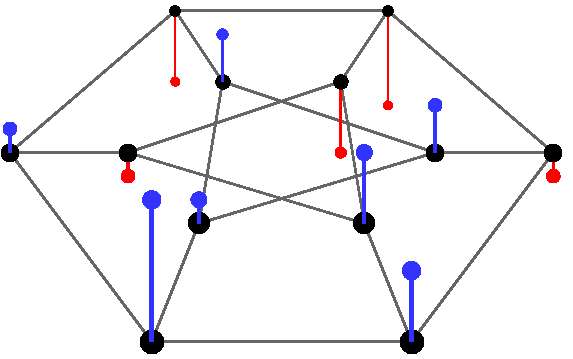
\includegraphics[width=0.35\linewidth]{Figures/signal_duher_graph_2.pdf}
	\floatsource
	\label{fig:duher}
\end{figure}

\subsection{The challenge of graph-like domains}

One of the reasons why GSP has been such a fertile field, allowing the birth of so many different problems and ideas, is that the definition of a signal over a graph leads to a series of obstacles when attempting to use even the most fundamental concepts of signal processing. Let us take the simple but elucidating example given by Shuman \emph{et al.}~\cite{shuman2013emerging}, and consider the unit shift to the right of a discrete-time signal $ x[n] $, which is done in digital signal processing by the simple variable substitution $ x[n-1] $. Good enough, but what does it mean to right-shift the signal in  Fig. \ref{fig:duher}, for example? Obviously the sense of right and left are meaningless for general graphs. On this problem, Shuman \emph{et al.} argue that a na\"ive choice would be to label the $ N $ graph vertices from $ v_0 $ to $ v_{N-1} $, so that the sample $ x[n] $ is assigned to vertex $ v_n $, for doing so would allow to define the shifted signal as the result of assigning $ x[n] $ to vertex $ v_{(n-1) \text{\,mod\,} N} $. Such an option, however, is not adequate, for its repeatability depends always on the way the vertices are labeled. This example illustrates how a concept in DSP as simple as signal translation may deserve a cautious study in GSP.


\section{Principles and definitions}
\label{sec:II}
The field of graph signal processing draws basic concepts from the classical theories of digital signal processing and graph theory, aiming to provide a cohesive and useful framework to tackle the aforementioned challenges. In this section, some of the main definitions found in this field are presented.


\subsection{Graph theory: a brief terminology}

A graph is commonly defined as the ordered pair  $ (\mathcal{V},\mathcal{E}) $, in which the set $ \mathcal{V} $ contains the so called graph \emph{vertices} and the set of \emph{edges} $ \mathcal{E} $ is a subset of $ \mathcal{V}^2 $ \cite{feofiloff2011introduccao}.  We will usually indicate by $ |\mathcal{V}| = N $\footnote{The set operator $ |\cdot| $ means the cardinality, or amount of elements, of the set.} and $ |\mathcal{E}| = E $ the number of vertices and edges of a graph, respectively. For our purposes it is convenient to represent a graph as the structure $ \mathcal{G} = \{\mathcal{V}, \mathbf{A}\} $, endowed with the (weighted) adjacency matrix $ \mathbf{A} $ which captures the vertex-to-vertex relations: if $ A_{i,j} \neq 0$, then there is an edge of weight $ A_{i,j} $ from the vertex $ v_j $ to $ v_i $. It is denoted by $ d_i^- $ the \emph{indegree} of vertex $ v_i $, consisting of the sum of weights of all incoming edges to vertex $ v_i $. Likewise, the \emph{outdegree} $ d^+_i $ is the sum of weights of edges departing from $ v_i $.

A graph is called \emph{undirected} if and only if its adjacency matrix is symmetric, in which case it is defined the \emph{degree} of vertex $ v_i $ as $ d_i^- = d_i^+ = d_i $. In this case, a graph is said to be \emph{d-regular} whenever all graph vertices have degree $ d $\label{pag:regular}. If $ \mathbf{A} $ is asymmetric, however, the respective graph is \emph{directed} and its pictorial representation depicts the edges as arrows, to account for the unidirectional relation between adjacent vertices. Examples of directed and undirected graphs are shown in Fig. \ref{fig:example_graphs}.

\begin{figure}
	\centering
    \caption{Examples of (a) directed and (b) undirected graphs, defined over the same vertex set.}
	\subfloat[]{
		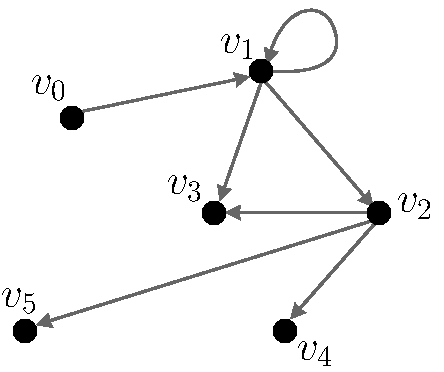
\includegraphics[width=0.25\linewidth]{Figures/example_graph_01_math.pdf}
	}~
	\subfloat[\label{fig:example_graphs_b}]{
		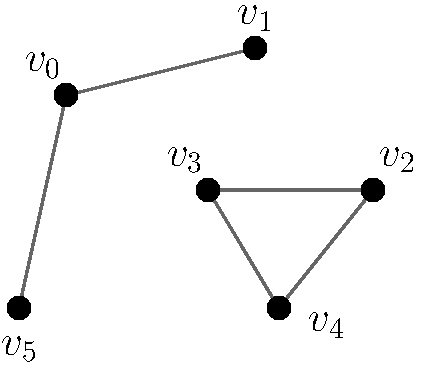
\includegraphics[width=0.25\linewidth]{Figures/example_graph_02_math.pdf}
	}
	\floatsource
	\label{fig:example_graphs}
\end{figure}

The adjacency matrix is the building block for one of the two main frameworks of GSP, what will be covered soon, but another matrix of great importance, mainly in the branch of GSP originated from spectral graph theory, is the Laplacian matrix
\begin{equation}
%\label{key}
\mathbf{L} = \mathbf{D} - \mathbf{A},
\end{equation}
with the \emph{degree matrix} $ \mathbf{D} $ being a diagonal matrix with $ d_i $ as the $ i $-th entry of its main diagonal. Depending on the context, $ \mathbf{D} $ may be taken as the indegree or outdegree matrix, although when the Laplacian matrix is used the graphs considered are often undirected.

A \emph{path} is a set of distinct edges (with the same orientation, if the graph is directed) linking distinct vertices, so that one could traverse all vertices by walking over the edges without ever repeat an edge or a vertex. A \emph{cycle} is like a path, except that it has equal starting and end vertices, and if a graph has a cycle it is called \emph{cyclic} (\emph{acyclic}, otherwise). If the cycle has only one edge, it is called a \emph{loop}. One refers to \emph{multiple edges} whenever a single pair of vertices is connected by two or more edges. An undirected graph is called \emph{simple} if it has no loops nor multiple edges.

A graph is said to be \emph{complete} if any two of its vertices are adjacent. Graph signal processing over such graphs may be extremely cumbersome, for the computational complexity of many of its techniques depends heavily on the number of graph edges. For most applications, it is desirable to have a small number of edges while keeping the graph \emph{connected}, i.~e., for any pair of vertices there exists a path connecting them.

A graph is said to be \emph{unweighted} if all its edges have unit weight. A \emph{subgraph} of $ \mathcal{G} $ is a graph $ \mathcal{G}' = (\mathcal{V}', \mathbf{A}')$ with edge set $ \mathcal{E}' $, in which $ \mathcal{V}' \subset \mathcal{V} $ and $ \mathcal{E}' \subset \mathcal{E} $. A \emph{connected component} of $ \mathcal{G} $ is a connected subgraph $ \mathcal{G}' = (\mathcal{V}', \mathbf{A}')$ in which any vertex in $ \mathcal{V}' $ is linked exclusively to another vertex also in $ \mathcal{V}' $. This is illustrated by Fig. \ref{fig:example_graphs_b}, in which the graph has two connected components.

\begin{figure}
	\centering
    \caption{(a) A graph and (b) the set of vertices $ \mathcal{N}(i,2) $ shown in red, with $ v_i $ being depicted in white. The edges linking $ v_i $ to the elements in $ \mathcal{N}(i,2) $ are also highlighted in red.}%
	\subfloat[\label{fig:k_hop_neighborhood_01}]{
		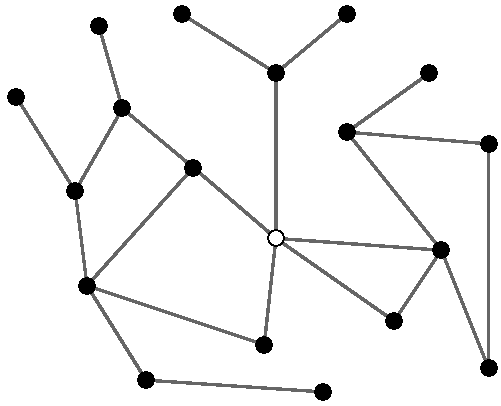
\includegraphics[width=0.25\linewidth]{Figures/k_hop_neighborhood_01.pdf}
	}~
	%	\qquad
	\subfloat[\label{fig:k_hop_neighborhood_02}]{
		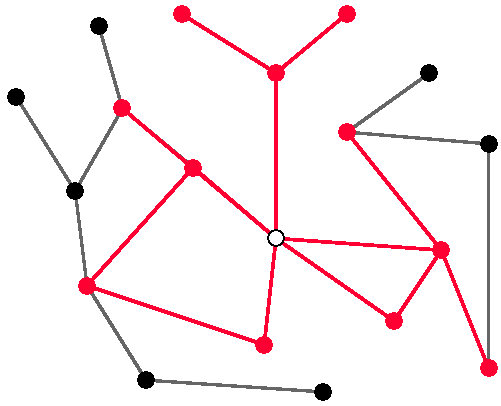
\includegraphics[width=0.25\linewidth]{Figures/k_hop_neighborhood_02.pdf}
	}
	%\hspace{0.2cm}%
	\floatsource
	\label{fig:k_hop_neighborhood}%
\end{figure}

The \emph{neighbourhood} of a vertex $ v_i $ is the set $ \mathcal{N}_i $ of all vertices adjacent to $ v_i $. Sometimes it is useful as well to denote by $ \mathcal{N}(i,K) $ the set of vertices connected to $ v_i $ through a path of length $ K $ or less. This notion is represented in Fig. \ref{fig:k_hop_neighborhood}.

The reader is encouraged to refer to this section whenever necessary. For a broader glossary with a solid introduction to graph theory, the reader may wish to read \cite{murty2008graph, chung1997spectral}.


\subsection{Defining a graph signal}

A signal $ \mathbf{s} $ defined over $ \mathcal{G} = \{\mathcal{V}, \mathbf{A}\} $, with $ |\mathcal{V}| = N $, is a discrete-domain function mapping the graph vertex set to a scalar set, usually the complex or real numbers,
\begin{equation}
\label{eq:def_signal}
s: \ \mathcal{V} \rightarrow \mathbb{C} \ | \ s(v_i) = s_i, \ i=0, \dots, N-1,
\end{equation}
so that the graph signal $ \mathbf{s} $ can be seen as a column vector in $ \mathbb{C}^N $ \emph{indexed by the vertices of} $ \mathcal{G} $. Once the vertices $ \mathcal{V} = \{v_1, \dots, v_N\}$ are clearly labeled, it is not ambiguous to represent the signal as the column vector $ \mathbf{s} = (s_0 \ s_1 \ \dots \ s_{N-1})^T$, $ s_i \in \mathbb{C} $, $ 0 \leq i \leq N-1 $.

\begin{figure*}
	\centering
    \caption{Examples of depictions of graph signals over (a) a directed ring graph,
		(b) an undirected regular grid graph and (c) a graph of cities from the Brazilian Northeastern region, over which was defined a signal of temperature measurements from February 1\textsuperscript{st} of 2012, retrieved from the
		\emph{Banco de Dados Meteorol\'ogicos para Ensino e Pesquisa} (BDMEP, freely translated as Meteorological Database for Teaching and Research), available at: \texttt{\url{http://www.inmet.gov.br/portal/index.php?r=bdmep/bdmep}}.}%
	\subfloat[\label{figa_graphs}]{
		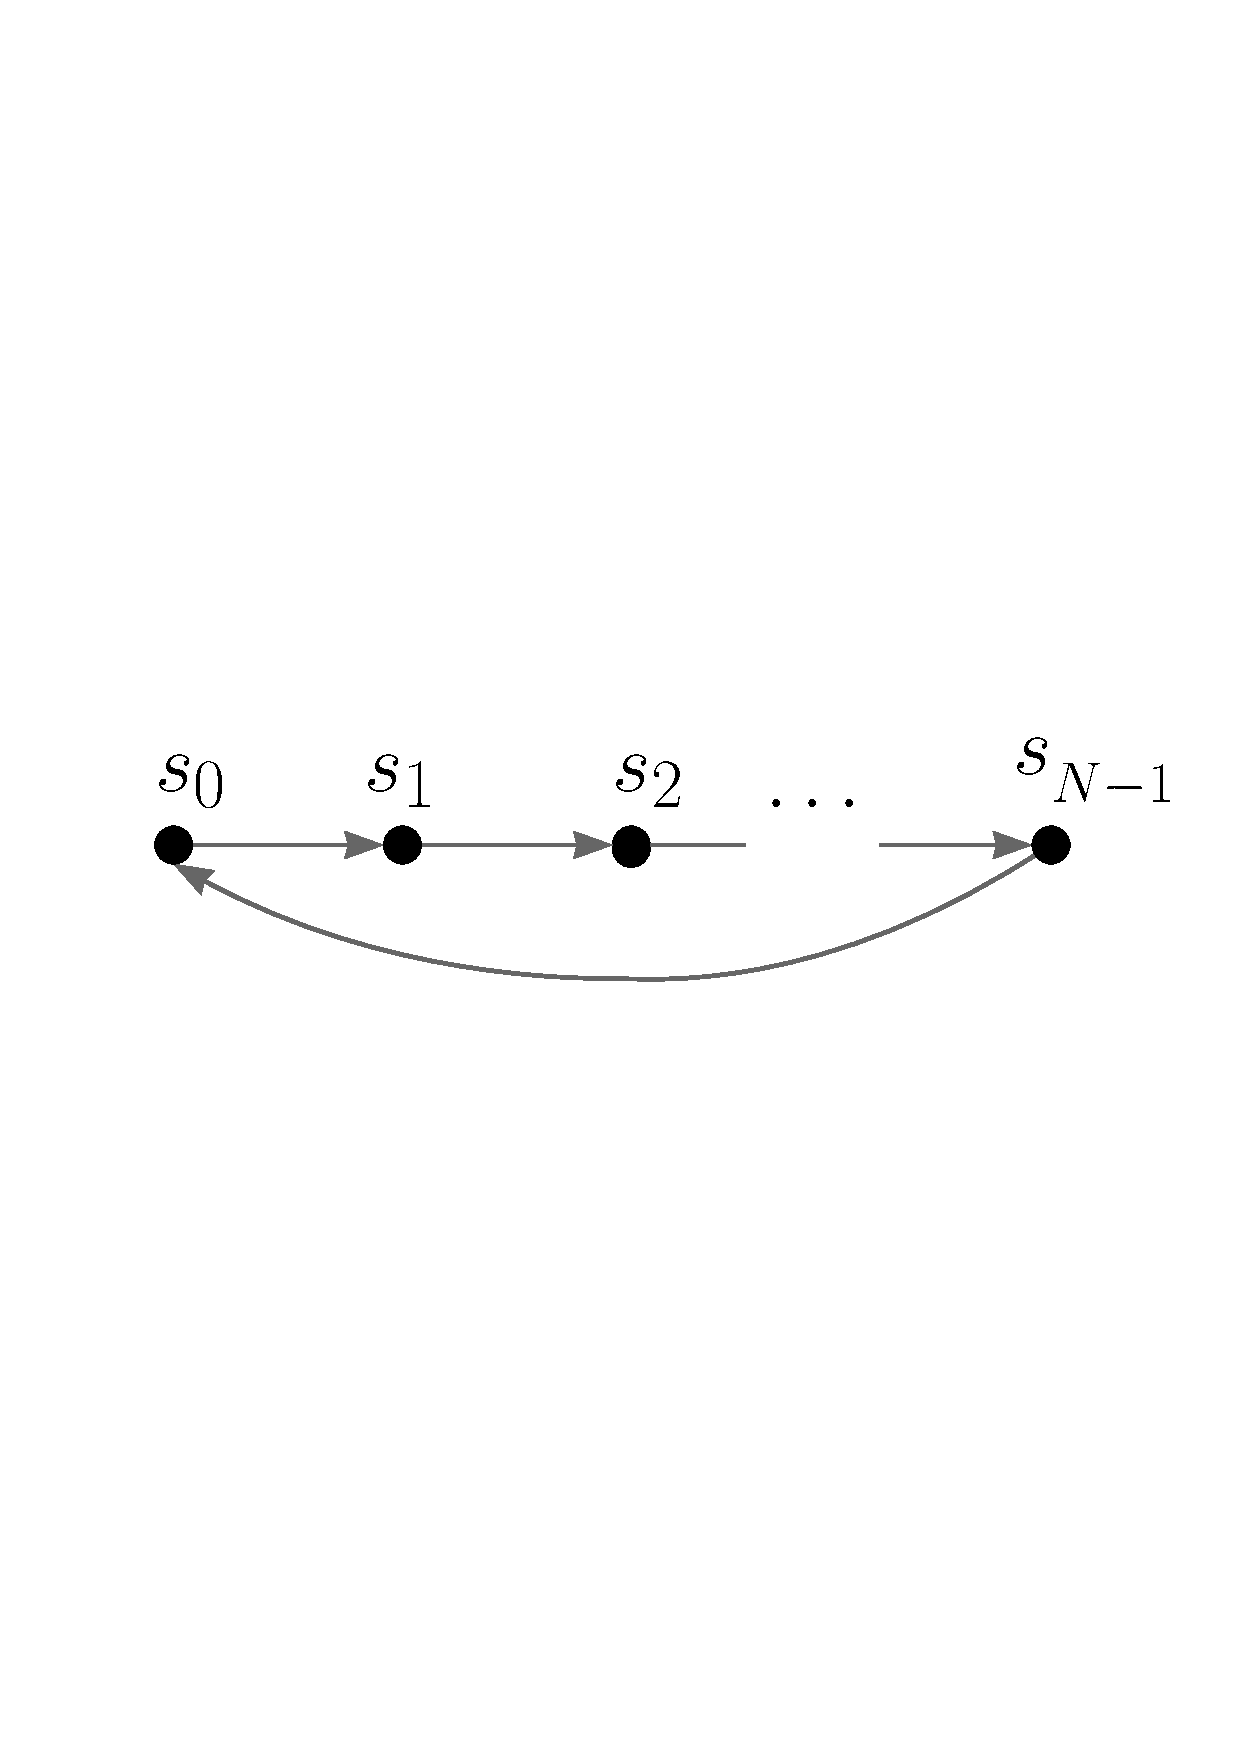
\includegraphics[width=0.25\linewidth]{Figures/signal_ring_graph_white_border.pdf}
	}
	\subfloat[\label{figb_graphs}]{
		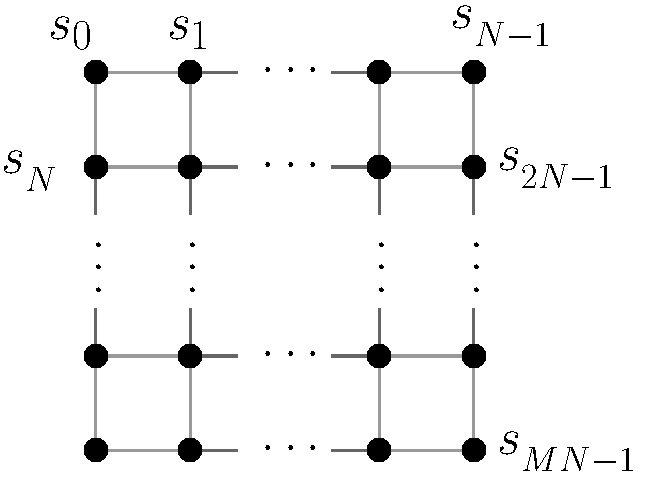
\includegraphics[width=0.25\linewidth]{Figures/image_graph.pdf}
	}%
	\subfloat[\label{figd_graphs}]{
		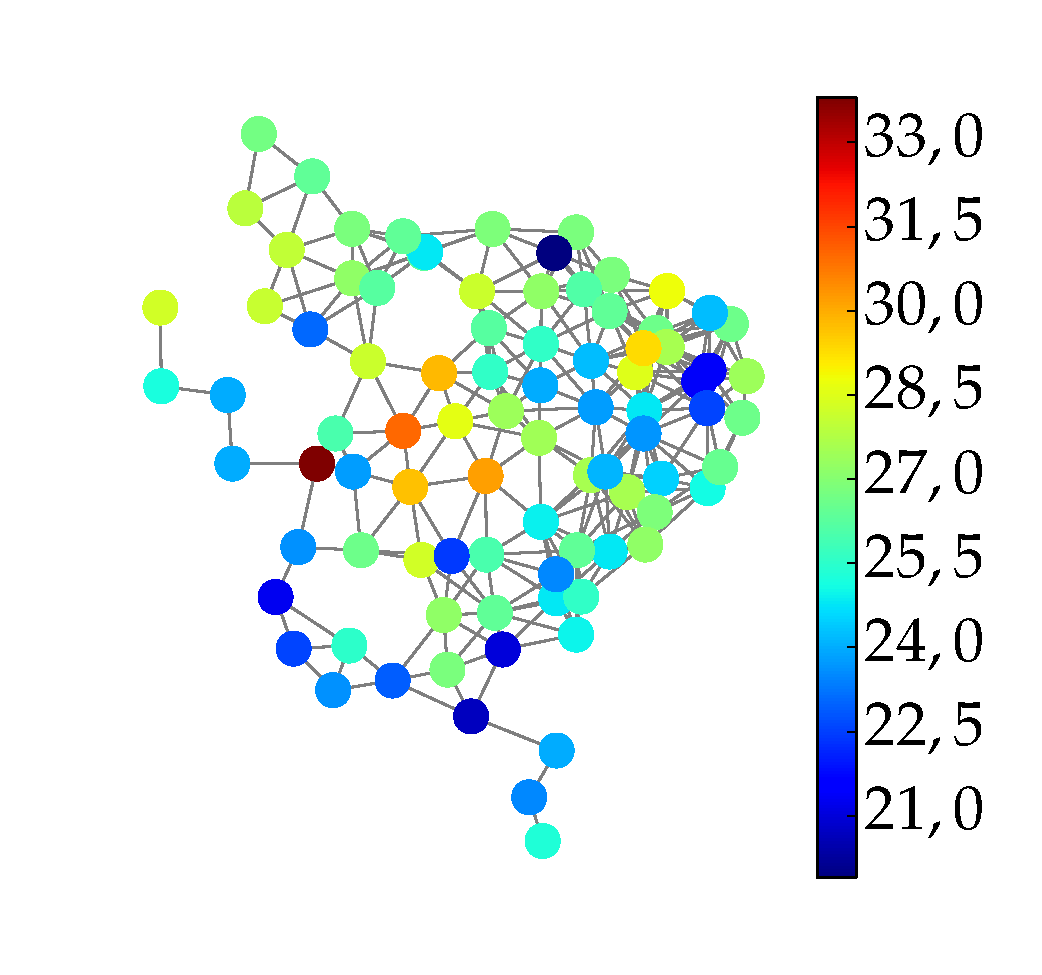
\includegraphics[width=0.3\linewidth]{Figures/temp_NE_stretched.pdf} }%
	\floatsource
	\label{fig:graphs}%
	\vspace{-0.2cm}
\end{figure*}

Fig. \ref{fig:graphs} provides examples of graph signal representations, in which the vertex labeling is omitted for the sake of simplicity, as it will be assumed that the signal sample $ s_i $ is assigned to vertex $ v_i $. The signal values are indicated in two manners: either by writing down its numerical value next to the respective vertex, or by using a pseudocolor scale, the latter of which is the scheme adopted throughout this paper.

It is crucial to stress a certain graph which links GSP to the classical DSP theory: the directed ring graph, shown in Fig. \ref{figa_graphs}, which models the finite-length discrete-time domain. Its directed edges model the causality of time domain, whereas the feedback edge accounts for the boundary condition of periodicity imposed by the DFT analysis. Other signals that arise in practical applications have the respective graphs easily identified: the rectangular lattice in Fig. \ref{figb_graphs}, for example, models the digital image domain \cite{sandryhaila2012nearest}, and Fig. \ref{figd_graphs} shows an example of signal defined over a mesh network of sensors, with the edges weighted using the inverse of the euclidian distance, which arises in many scenarios such as IoT applications.

\begin{figure*}
	\centering
    \caption{The same signal defined over two similar graphs, one of them being (a) the undirected ring graph. In (b) and (d) are depicted the Fourier spectra of the signals in (a) and (c), respectively.}%
	\begin{minipage}[c]{0.24\linewidth}
		\subfloat[\label{fig:diff_struct_a}]{
			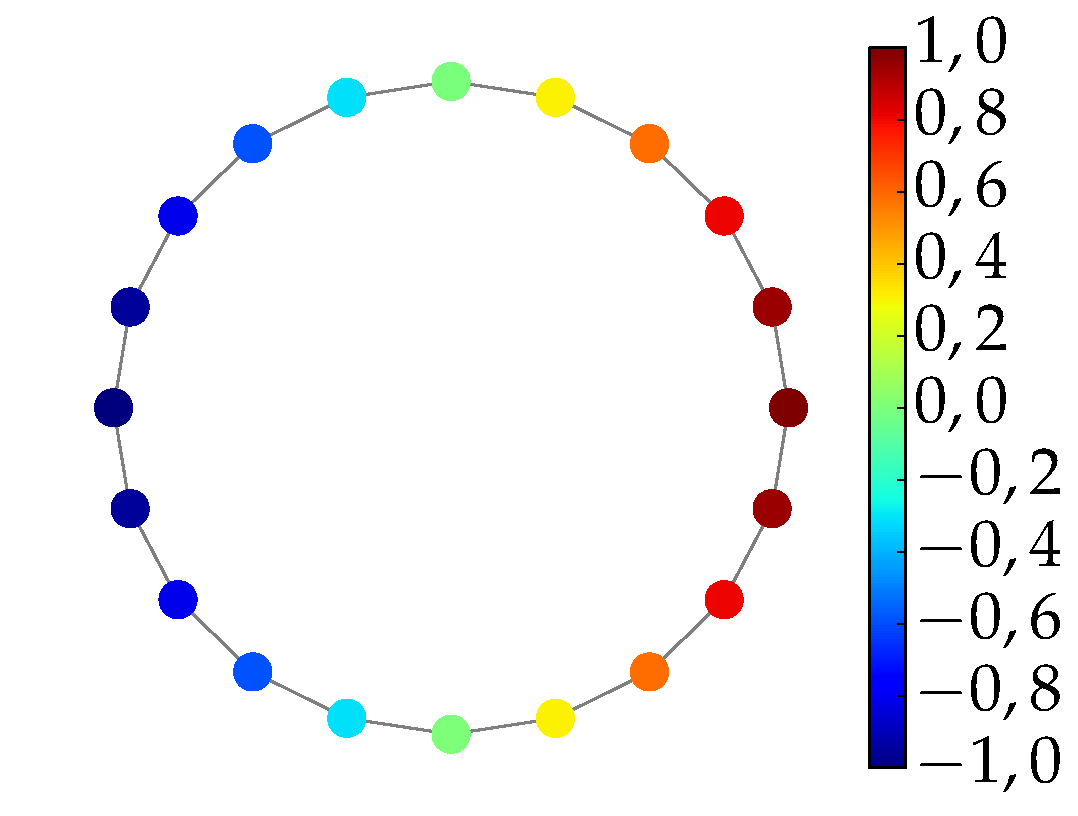
\includegraphics[width=\linewidth]{Figures/ring_different_structure_01.pdf}
		}
	\end{minipage} %
	\begin{minipage}[c]{0.24\linewidth}
		\subfloat[\label{fig:diff_struct_c}]{
			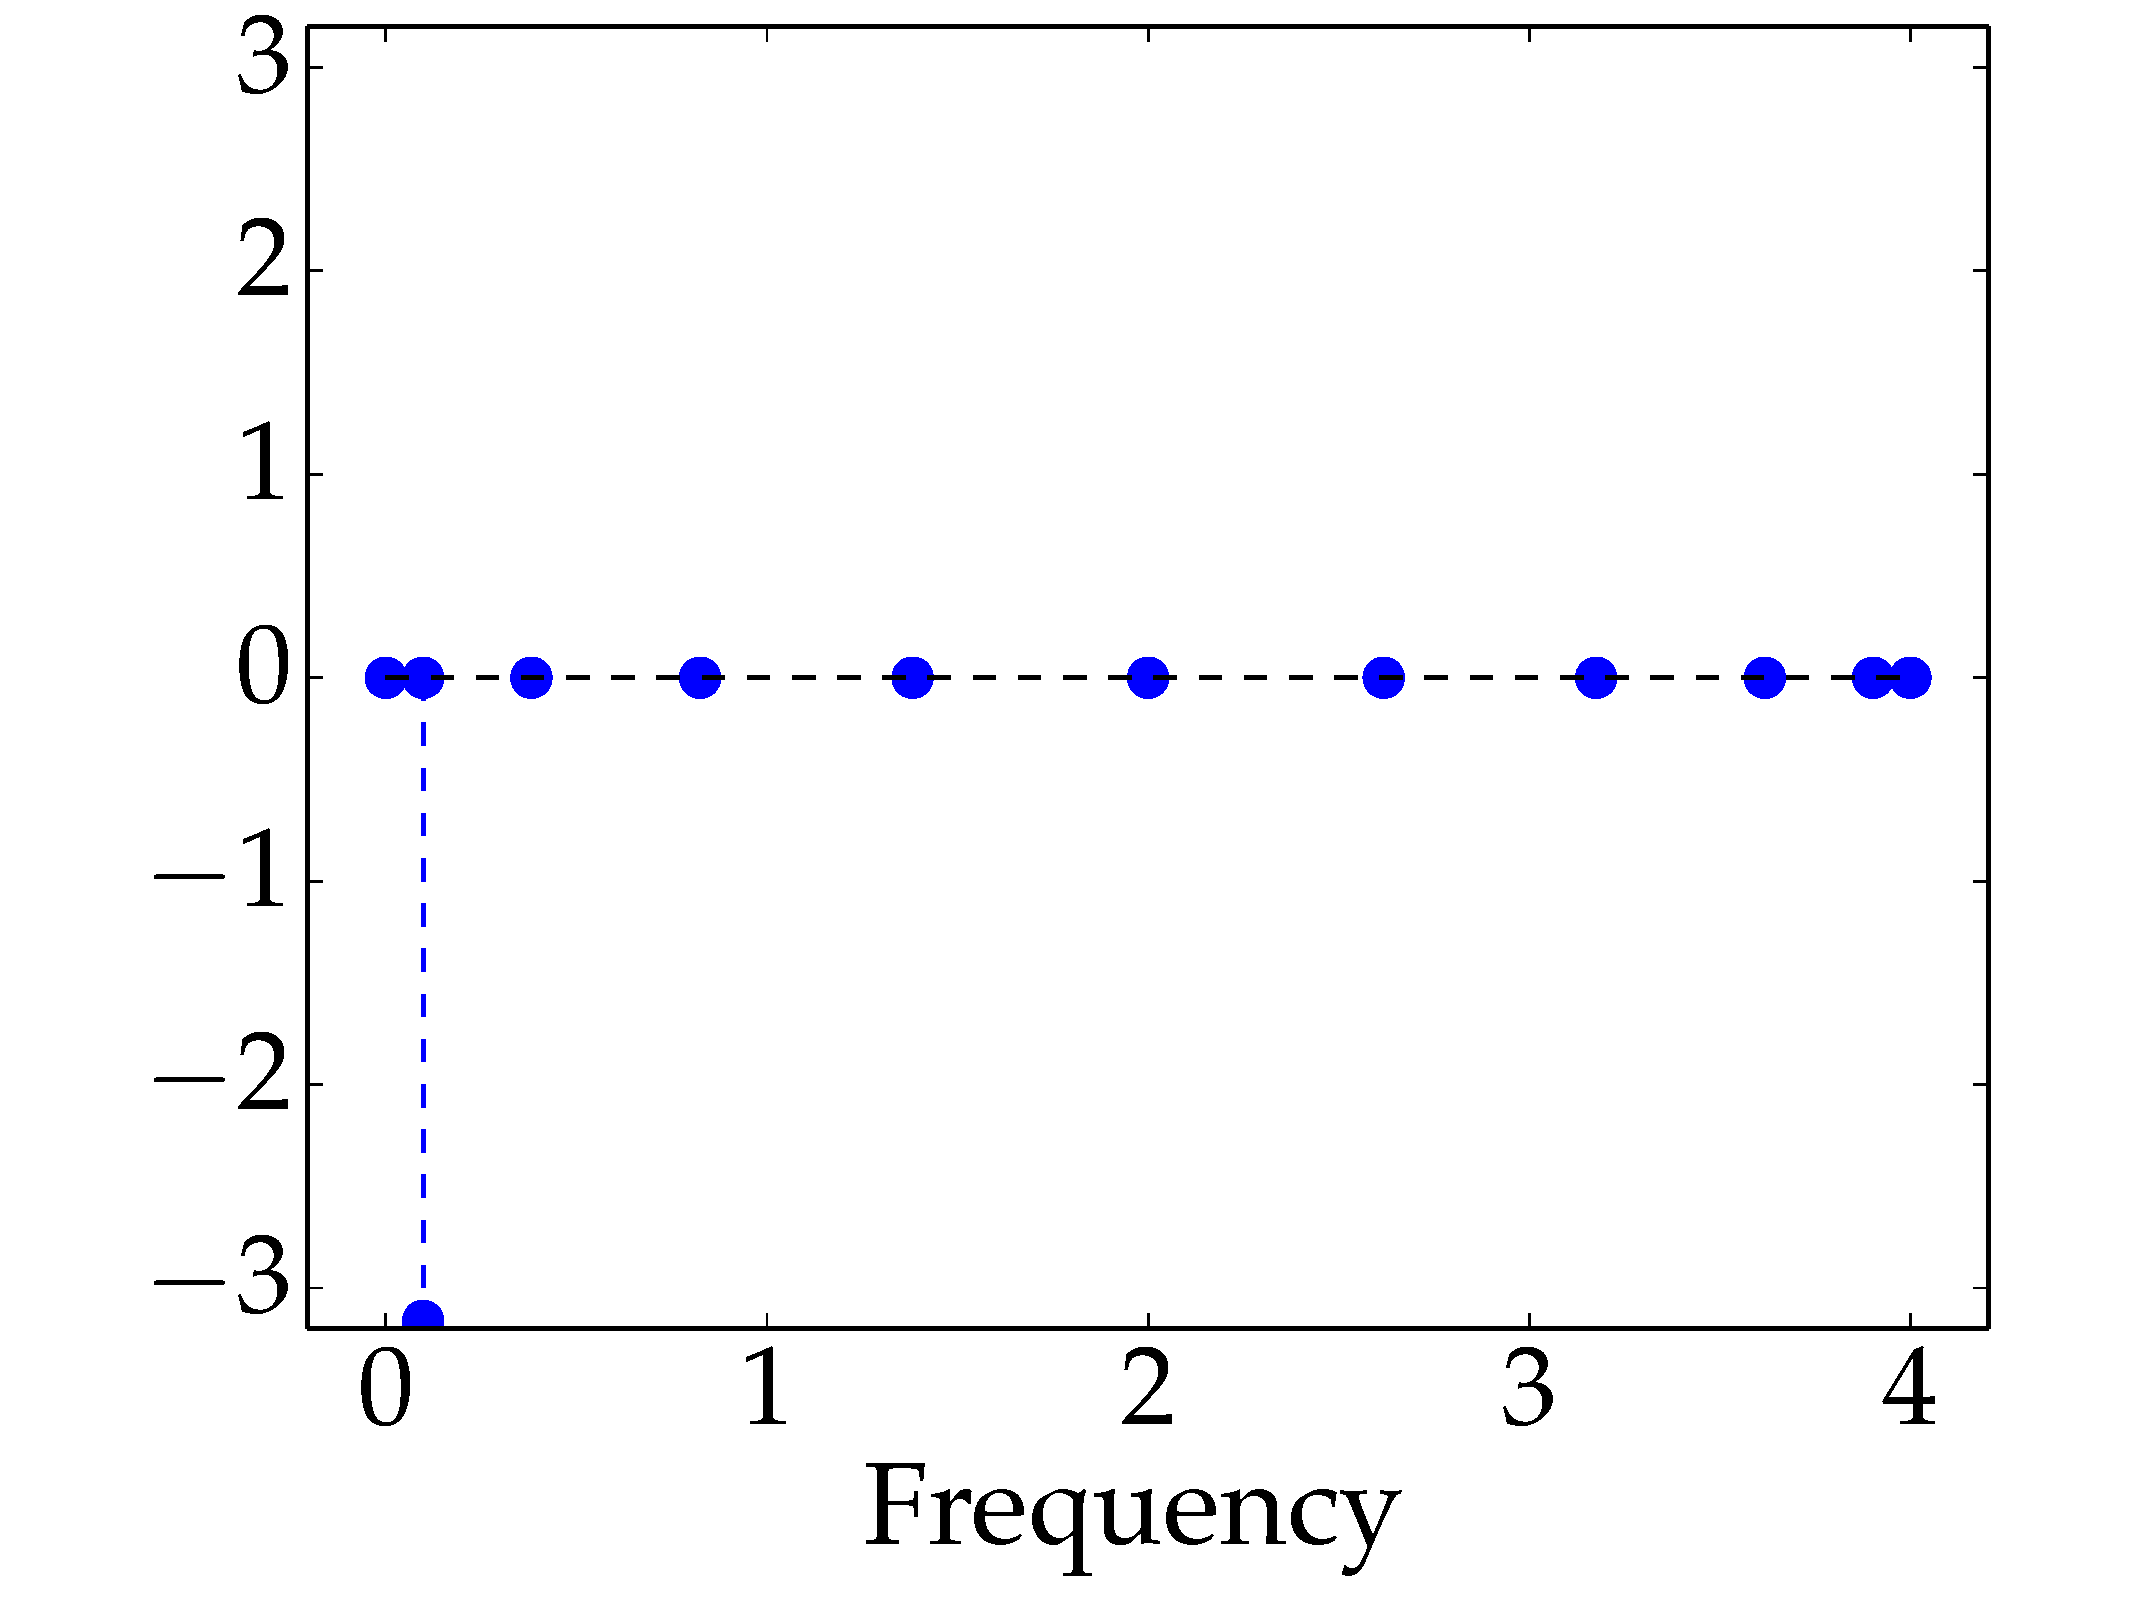
\includegraphics[width=\linewidth]{Figures/ring_different_structure_01_spectrum_EN.pdf}
		}
	\end{minipage}%
	\begin{minipage}[c]{0.24\linewidth}
		\subfloat[\label{fig:diff_struct_b}]{
			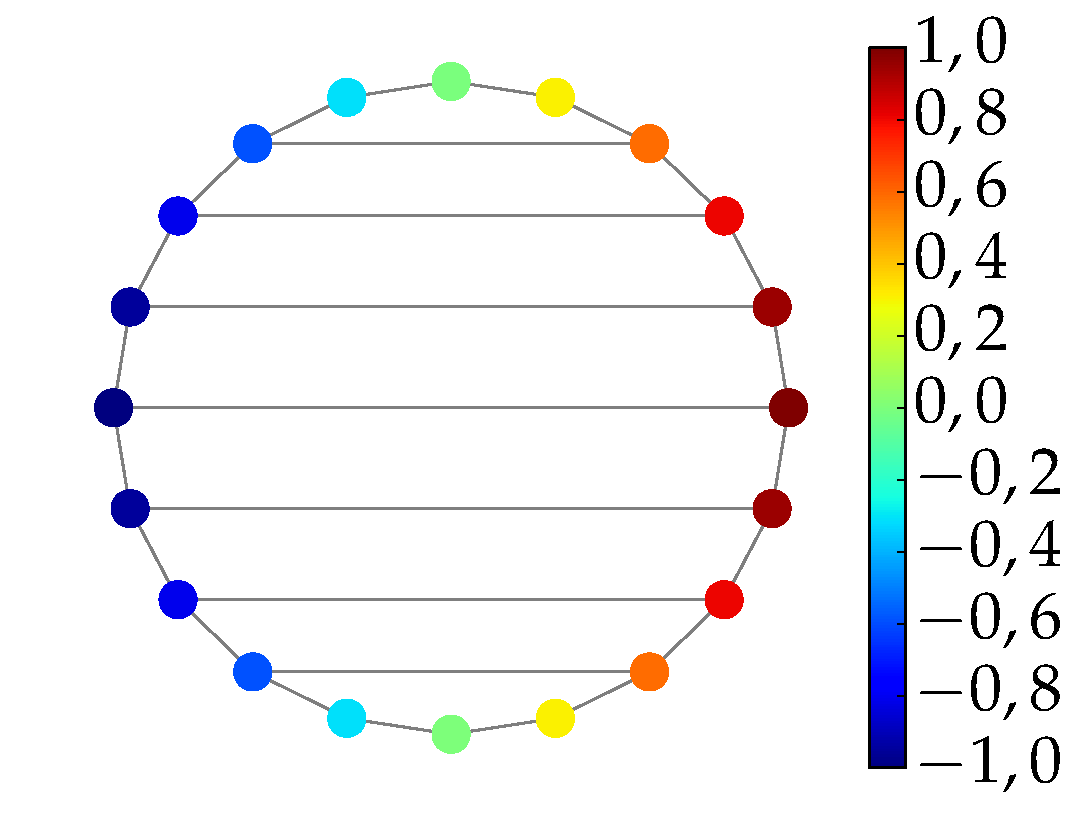
\includegraphics[width=\linewidth]{Figures/ring_different_structure_02.pdf}
		}~
	\end{minipage}%
	\begin{minipage}[c]{0.25\linewidth}
		\subfloat[\label{fig:diff_struct_d}]{
			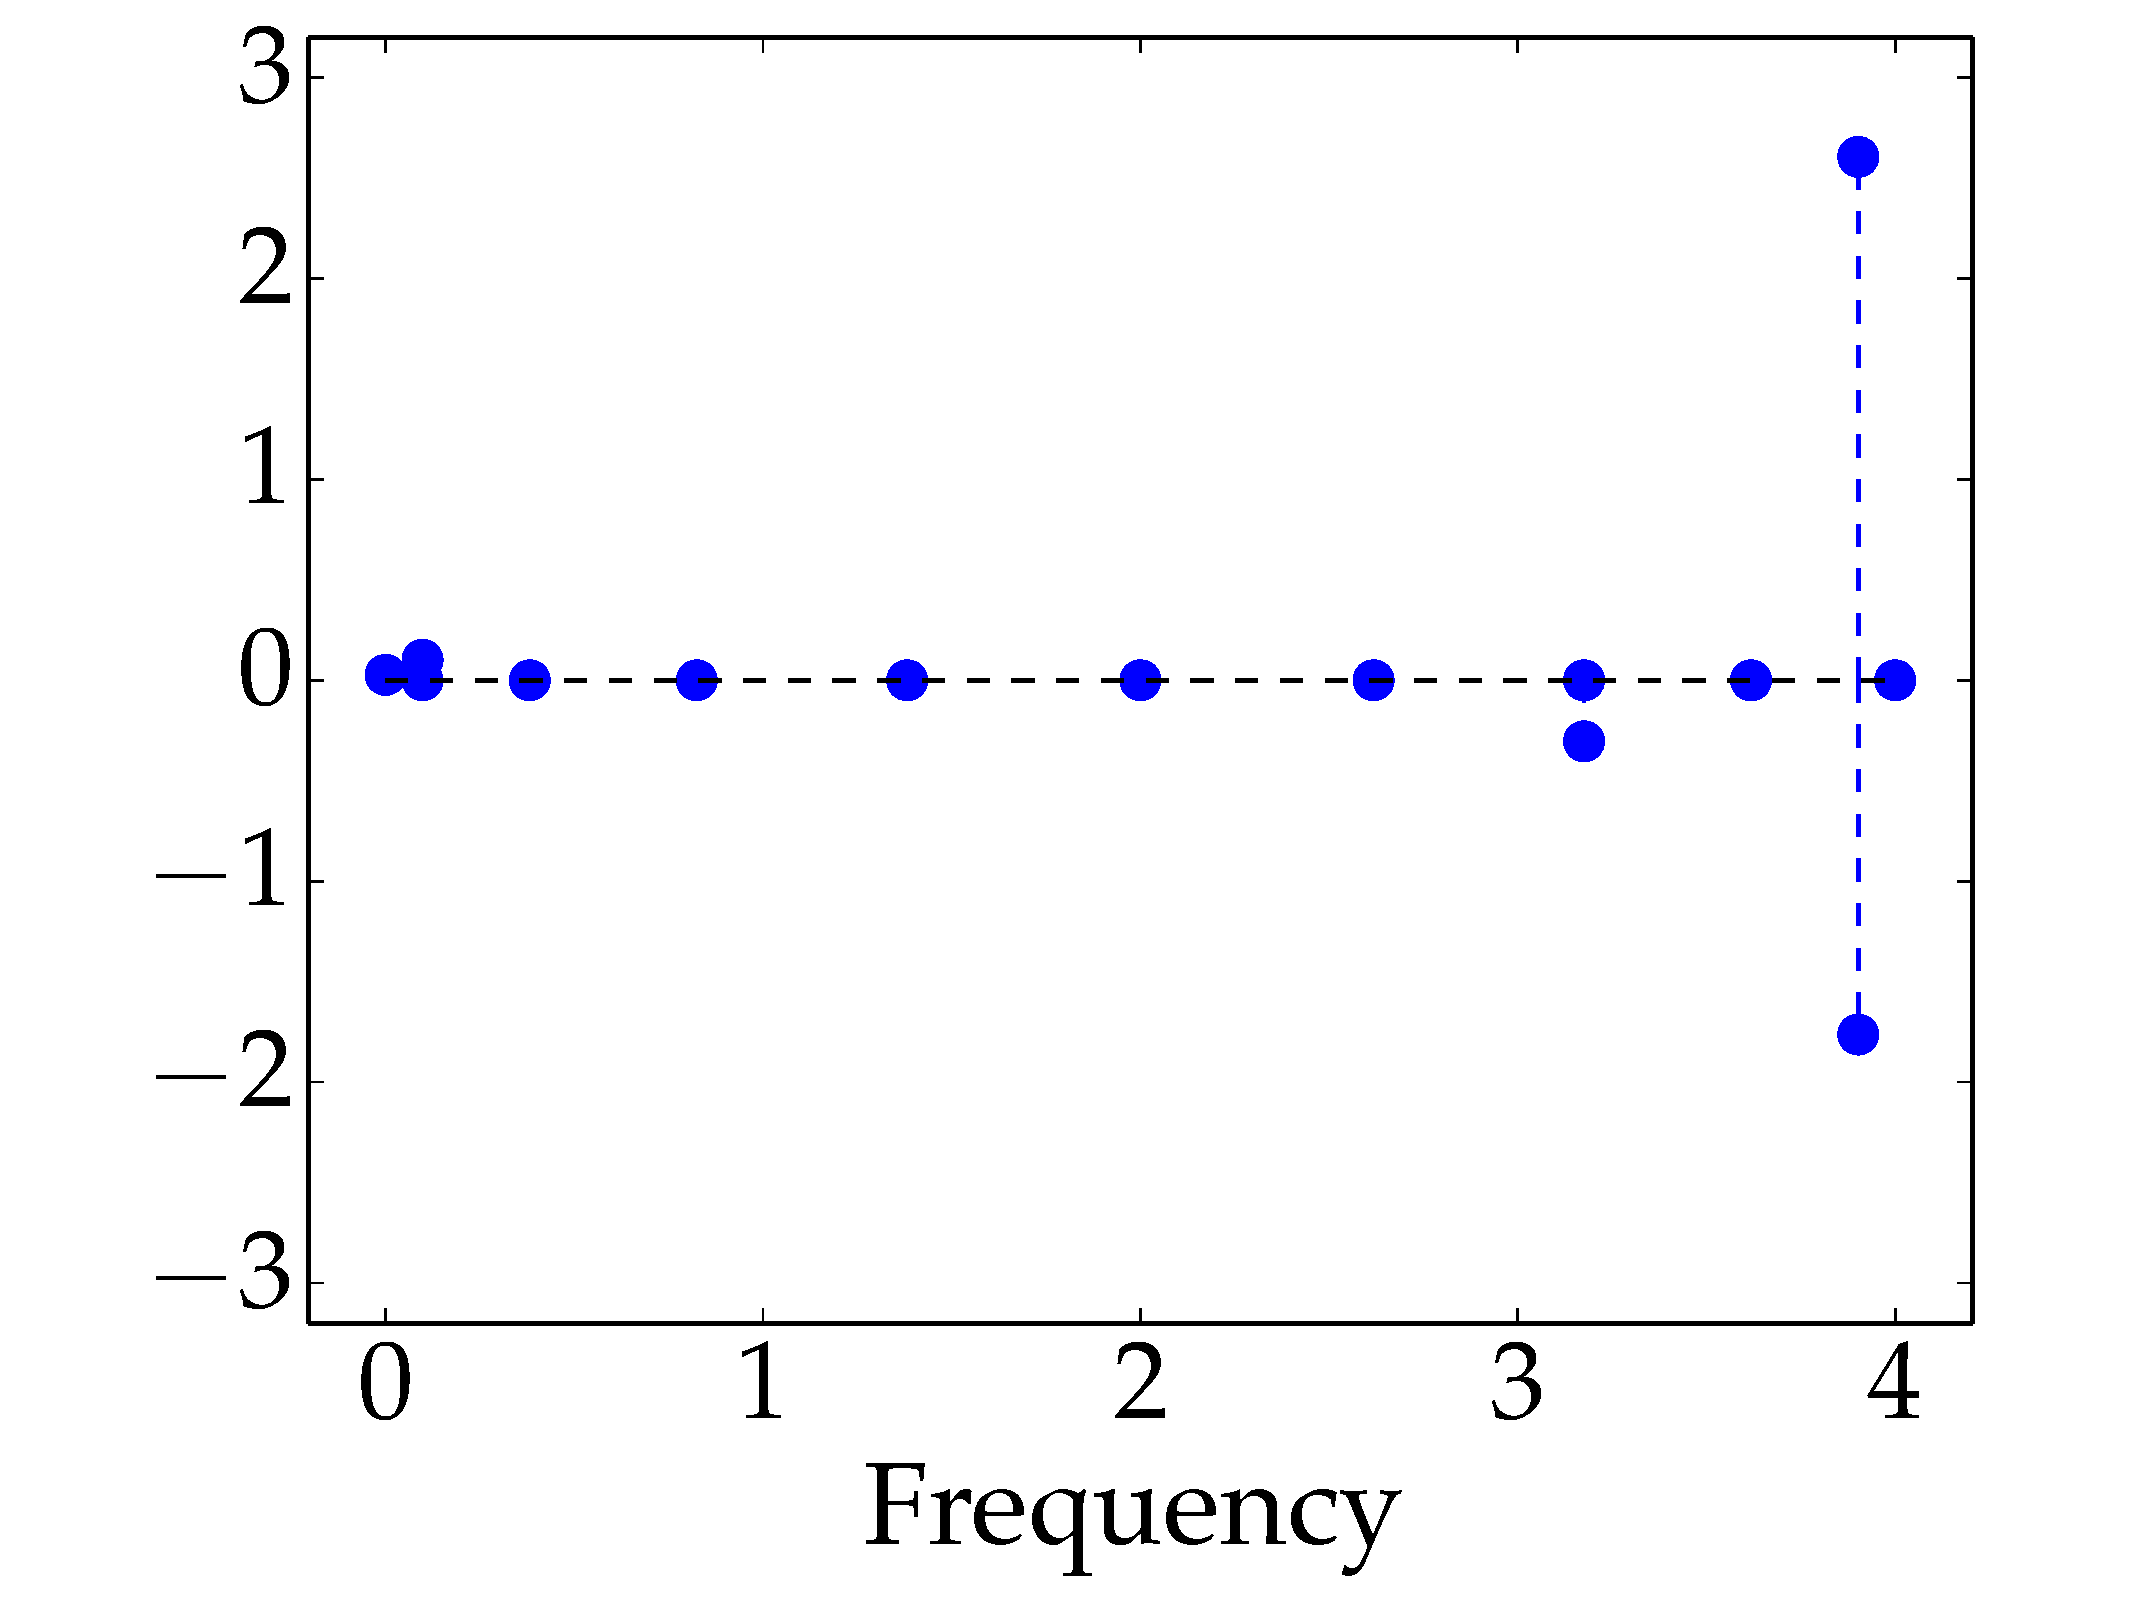
\includegraphics[width=\linewidth]{Figures/ring_different_structure_02_spectrum_EN.pdf}
		}
	\end{minipage}%
	\floatsource
	\label{fig:diff_struct}%
	\vspace{-0.2cm}
\end{figure*}

The spectral characteristics of a signal depend heavily on the domain over which it is defined, but one does not need to acknowledge this in the context of DSP, for in this case the domains are always regular and uniform.\footnote{One could argue that, in the theory of \emph{nonuniform sampling}, the signal is defined over an irregular domain, since the samples may be randomly spaced. Even in this case, however, the classical techniques still aim to \emph{recover} the signal so as to represent it in its usual -- and \emph{uniform} -- domain.
}
From the classical theory, the common understanding states that a signal has mostly low frequencies if adjacent samples have similar values, and high frequencies otherwise. When dealing with signals defined over graphs, it is clear that the adjacency relations depend on the graph topology, and therefore one may foresee that \emph{the same signal may present different spectra when defined over different graphs}. This intuition is visually confirmed (and will soon be mathematically proved) in Fig. \ref{fig:diff_struct}, which depicts a signal and its spectra\footnote{These spectra were obtained using the Laplacian matrix as a graph shift operator, not the adjacency matrix. The reader should not bother with the differences for now, it suffices to know that the spectra can be read as usual: frequencies increase as you move to the right on the frequency axis. In other words, any low-pass signal will have most of its energy lying on the left-hand side of the spectrum.} when two different graphs are taken as domain. The reader may notice that, in Fig. \ref{fig:diff_struct_b}, the samples with highest values are adjacent to the ones with small values, what causes the highest concentration of energy to be in the highest frequencies. The opposed behavior is observed in the signal defined over the undirected ring graph in Fig. \ref{fig:diff_struct_a}.

\subsection{Graph inference}
\label{subsec:inferindo}

Some contexts in which GSP is applied do not provide clear information on \emph{how the underlying graph is structured}. For example, let us suppose the temperature data (or any other data in fact) of some Brazilian Northeastern cities will be treated using GSP. How is one supposed to weight the graph edges, and before this, how does one decide which vertices to connect? Is the graph shown in Fig. \ref{figd_graphs} the only option? Clearly not. Although generally the problem of graph inference is complex, this type of geography-based graph has an adequate method of topology estimation.

The general ideia is that, if there is a clear metric to evaluate the \emph{expected} similarity between samples as a function of the available information regarding the respective vertices, then this metric may be used to generate the edge weight and a threshold is set so that any weight below this value causes the respective edge to be eliminated. In the case of vertices which have geographic location, the euclidian distance may be used as the metric because vertices that are closer together are (usually) \emph{expected} to have similar signal samples, and therefore the adjacency matrix of the underlying graph may have entries given by
\begin{equation}
\label{eq:weights}
A_{ij} =
\begin{cases}
\displaystyle
\exp \left(- \frac{\text{dist}^2(v_i, v_j)}{2 \theta^2}\right)& \text{ if } \text{dist}(v_i, v_j) < T \\ 
0 & \text{ otherwise},
\end{cases}
\end{equation}
as used in \cite{shuman2013emerging}. The choice of the parameters $ T $\footnote{$ T $ indicates a distance threshold above which we set the edge weight to zero, effectively leaving the vertices unlinked. This means that the distance between them is assumed to be too high for any significant interdependence to exist.} and $ \theta $ (standard deviation of the distribution), and of how to use the metric (in this case, inside a Gaussian distribution), are dictated by the application and by the analyst experience. 

However, if there is an isolated vertex, far from the others, the use of (\ref{eq:weights}) may lead to a compromise between keeping the graph connected and obtaining a sparse adjacency matrix, since imposing connectivity to the graph in this case implies increasing $ T $, and therefore having many edges. To deal with this problem and still have a good representation of the underlying graph, one alternative is to connect a vertex to its $ K $ closest neighbours (setting $ K $ to an appropriate value, according to the context) and weight the edges using the Gaussian distribution in (\ref{eq:weights}).

As previously discussed, these methods require an adequate metric to evaluate the expected similarity between samples in the graph vertex, but given the diverse areas in which graph signals may arise, estimating the topology of the  underlying graph constitutes a challenge of its own \cite{mei2016signal,Sardellitti2016}.

\section{Formulating GSP based on the graph adjacency matrix}
\label{sec:DSPG}

In 2008, P\"uschel and Moura published their \emph{algebraic signal processing} (ASP) theory \cite{puschel2008time,puschel2008space}, which expands DSP by looking at it from an algebraic point of view: each signal processing theory is studied as a triple $ (\mathscr{A}, \mathscr{M}, \Phi) $ consisting of an algebra $ \mathscr{A} $ (a vector space endowed with multiplication between vectors), an $ \mathscr{A} $-module $ \mathscr{M} $ (a vector space over the same base field as $ \mathscr{A} $ which admits left-multiplication by elements of $ \mathscr{A} $) and a linear transformation $ \Phi $. $ \mathscr{A} $ is called the filter space, $ \mathscr{M} $ is the signal space and $ \Phi $ is the Fourier transform (homomorphism over $ \mathscr{M} $) associated with the structure.

When these authors drew inspiration from ASP to develop their GSP theory, the starting point was necessarily to find (better, to define) the unit shift operator of graph signals, the reason being that such an operator in ASP is the building block of the algebra $ \mathscr{A} $ (as, for example, the unit delay $ z^{-1} $ is the building block for filters of discrete-time and finite-length signals $ \mathscr{A}  = \{ \sum_{\ell=0}^{N-1} h_\ell z^{-\ell} | h_\ell \in \mathbb{C} \}$). To do so, the shift of discrete-time signals, defined over directed ring graphs, was investigated.

By inspection of the \emph{adjacency matrix} of the directed ring graph (Fig. \ref{figa_graphs}),
\begin{equation}\label{eq:C}
\mathbf{C} =
\begin{bmatrix}
&  &  &   1\\ 
1 &  &   & \\ 
&   \ddots &  & \\ 
&  &   1 & 
\end{bmatrix},
\end{equation}
it was noticed that the unit (circular) shift of discrete-time signals is precisely the left-multiplication by $ \mathbf{C} $, for a given discrete-time signal $ \mathbf{x} = (x_0 \ x_1 \ \dots \ x_{N-1})^T $,
\begin{equation}\label{eq:unit_shift}
\mathbf{C}\mathbf{x} =
\begin{bmatrix}
&  &  &   1\\ 
1 &  &   & \\ 
&   \ddots &  & \\ 
&  &   1 & 
\end{bmatrix}
\begin{bmatrix}
x_0 \\ x_1 \\ \vdots \\ x_{N-1}
\end{bmatrix} =
\begin{bmatrix}
x_{N-1} \\ x_0 \\ \vdots \\ x_{N-2}
\end{bmatrix} \overset{\Delta}{=} \mathbf{x}^{\langle 1 \rangle},
\end{equation}
and the generalization followed: \emph{the graph unit shift was defined as the left-multiplication by the graph adjacency matrix}.

In other words, for a signal $ \mathbf{x} $ defined over the graph $ \mathcal{G} = \{\mathcal{V}, \mathbf{A}\} $, the adjacency matrix $ \mathbf{A} $ acts as a \emph{filter} which ``delays'' (i.~e., translates in the vertex domain) the graph signal $ \mathbf{x} $ (represented here as a column vector) by one unit, producing the delayed version represented hereinafter by $ \mathbf{x}^{\langle 1 \rangle} = \mathbf{A} \mathbf{x}$.

\subsection{Graph filters}
\label{subsec:filtros}

Seeing the adjacency matrix as a filter suggested the general definition of \emph{graph filter} as any matrix $ \mathbf{H} \in \mathbb{C}^{N \times N} $ \cite{sandryhaila2013filters}, which preserves the necessary property that the output of a filter (i.~e., the matrix-vector product) is a signal (i.~e., a column vector). Such a definition implies that \emph{linearity} is always valid for graph filters, since the distributivity of matrix multiplication with respect to matrix addition guarantees that
\begin{equation}
%\label{key}
\mathbf{H} (\alpha_1 \mathbf{x}_1 + \alpha_2 \mathbf{x}_2) =  \alpha_1 \mathbf{H} \mathbf{x}_1 + \alpha_2 \mathbf{H}  \mathbf{x}_2.
\end{equation}

The next desirable property would be \emph{shift invariance}, analogous to the classical time invariance of DSP, and this means that filtering and shifting should commute. In other words, for a graph filter $ \mathbf{H} $ to be \emph{linear and shift invariant} (LSI) it is required that
\begin{equation}
\label{eq:lsi_def}
\mathbf{A} \mathbf{H} \mathbf{x} = \mathbf{H} \mathbf{A} \mathbf{x}, \ \ \forall \mathbf{x} \in \mathbb{C}^N
\Rightarrow
\mathbf{A} \mathbf{H} = \mathbf{H} \mathbf{A}.
\end{equation}
% $ \mathbf{A} \mathbf{H} \mathbf{x} = \mathbf{H} \mathbf{A} \mathbf{x} \ \forall \mathbf{x}$, and therefore $ \mathbf{A} \mathbf{H} = \mathbf{H} \mathbf{A}$.
% Sandryhaila and Moura have shown \cite{sandryhaila2013discrete,sandryhaila2014big} that LSI filters can be represented as polynomials $ h(\cdot) $ evaluated over $ \mathbf{A} $,
% \begin{equation}
% \label{eq:filter_poly}
% h(\mathbf{A}) = \sum_{\ell=0}^{L-1} h_\ell \mathbf{A}^\ell,
% \end{equation}
% with $ L $ smaller than or equal to the degree of the minimal polynomial of $ \mathbf{A} $, i.~e., LSI filters are finite power series on the shift operator, exactly as it happens in DSP, in which LTI filters have polynomial representations on $ z^{-1} $.
The following theorem establishes an important property satisfied by every LSI filter~\cite{sandryhaila2013discrete} .
\vspace{0.2cm}
\begin{theorem}
\label{theo:01}
Let $ \mathbf{A} $ be the adjacency matrix of a graph. Let us assume that the characteristic polynomial $char_{\mathbf{A}}(x)$ of $\mathbf{A}$ coincides with the respective minimal polynomial $m_{\mathbf{A}}(x) $. Therefore, $ \mathbf{H} $ is an LSI filter if and only if $ \mathbf{H} $ is a polynomial in $ \mathbf{A} $, i.~e.
\begin{equation}\label{eq:filtro}
\mathbf{H} = h(\mathbf{A}) = \sum_{\ell=0}^{L} h_\ell \mathbf{A}^\ell,
\end{equation}
where $ \mathbf{A}^0 $ is the identity matrix and $ L < \deg(m_{\mathbf{A}}) $.
\end{theorem}

The assumption on $char_{\mathbf{A}}(x)$ and $m_{\mathbf{A}}(x)$ in Theorem~\ref{theo:01} does not hold for all adjacency matrices $\mathbf{A}$. Nevertheless, the result in the referred theorem can be extended to all matrices using the concept of \emph{equivalent graph filters}, as clearly explained in~\cite{sandryhaila2013filters}. As a consequence, for any graph $\mathcal{G} = \{\mathbf{A}, \mathcal{V}\}$, every LSI filter has polynomial representation in $\mathbf{A}$. In this sense, Theorem~\ref{theo:01} suggests a convenient analogy with the classical DSP, since every filter for discrete-time signals can be represented as polynomials evaluated in $ z^{-1} $, the unit delay, via the $z$-transform of its impulse response.

\subsection{Graph Fourier transform}

The topic of spectral analysis is key in signal processing. When studying how this would be implemented in the scope of GSP, the authors started by looking at the classical Fourier transform as a signal decomposition into a basis of eigenfunctions of the LTI filtering \cite{oppenheim1997signals}, i.~e., the basis of complex time exponentials. From that point, the generalization to GSP was clear: the \emph{graph Fourier transform} (GFT) was defined as the decomposition of a graph signal into a basis of eigenvectors of LSI filtering.\footnote{One may wish to distinguish between the different implementations of the GFT regarding the choice of graph shift operator. Unless clearly stated otherwise, this chapter considers it to be always the graph adjacency matrix, but other popular option is the graph Laplacian, as already mentioned. In this regard, the reader even may find the terms GSP\textsubscript{A} and GSP\textsubscript{L} in previous publications \cite{ribeiro2018}, making the distinction clear.}

Let us take the graph $ \mathcal{G} = \{\mathcal{V}, \mathbf{A}\} $, $ |\mathcal{V}| =N $. If $ \mathbf{A} $ is diagonalizable,\footnote{If not, the reasoning may be replicated using the Jordan decomposition of $ \mathbf{A} $ and the set of generalized eigenvectors \cite{deri2017spectral}.} then one may write
\begin{equation}\label{eq:gft_01}
\mathbf{A} = \mathbf{V} \mathbf{\Lambda} \mathbf{V}^{-1},
\end{equation}
in which $ \mathbf{V} $ contains the $ N $ eigenvectors of $ \mathbf{A} $ in its columns,
\begin{equation}\label{eq:gft_02}
\mathbf{V} = (\mathbf{v}_0 \ \mathbf{v}_1 \ \dots\ \mathbf{v}_{N-1}).
\end{equation}

Since LSI filters are polynomials in $ \mathbf{A} $, and since a matrix and its powers share the same set of eigenvectors, the columns of $ \mathbf{V} $ form a basis of vectors invariant to LSI filtering. Besides, given that the subspaces generated by the linearly independent eigenvectors of a same eigenvalue of $ \mathbf{A} $ are irreducible, have null intersection and the dimensions of all subspaces add to $ N $ \cite{sandryhaila2013gft}, $ \mathbf{V} $ provides a basis which is invariant to LSI filtering for the space of signals defined over $ \mathcal{G} $.

Therefore, a signal $ \mathbf{x} $ may be decomposed into its components with respect to $ \mathbf{V} $ as
\begin{align}\label{eq:GFT_inv}
\mathbf{x} &= \widehat{x}_0 \mathbf{v}_0 + \dots + \widehat{x}_{N-1} \mathbf{v}_{N-1} \notag \\
&= \mathbf{V} (\widehat{x}_0 \ \widehat{x}_1 \ \dots \ \widehat{x}_{N-1})^T \notag \\
&= \mathbf{V} \widehat{\mathbf{x}} \overset{\Delta}{=} \textrm{GFT}\{\mathbf{x}\},
\end{align}
and this is the synthesis equation of the GFT. The analysis equation follows,
\begin{equation}\label{eq:GFT_fwd}
\widehat{\mathbf{x}} = \mathbf{V}^{-1} \mathbf{x} \overset{\Delta}{=} \textrm{GFT}^{-1}\{\mathbf{x}\}.
\end{equation}

It has been emphasized that the directed ring graph is the link between GSP and DSP, because it models the discrete-time domain. This provides a way of checking how consistent with the classical theory are the proposed GSP tools. When investigating how the GFT would act upon discrete-time signals, one should first diagonalize the adjacency matrix $ \mathbf{C} $ of the directed ring graph, given by (\ref{eq:C}). Since it is circulant, it is known to be diagonalized by the DFT matrix $ \mathbf{F} $, with entries $ F_{n,k} = \exp \left( -j\frac{2 \pi}{N} nk \right) $, which contains in its \emph{rows} the DFT eigenvectors. The calculation of the characteristic polynomial of $ \mathbf{C} $,
\begin{equation}
%\label{key}
p_{\mathbf{C}}(\lambda) = \text{det} (\lambda \mathbf{I} - \mathbf{C}) =
\begin{vmatrix}
\lambda &  &  &   -1\\ 
-1 & \lambda &   & \\ 
&   \ddots & \ddots & \\ 
&  &   -1 & \lambda
\end{vmatrix}
=\lambda^N - 1,
\end{equation}
shows that its eigenvalues are the $ N $ complex roots of unity. Setting these eigenvalues as the entries of a diagonal matrix $ \mathbf{\Lambda}_{\mathbf{C}} $, the eigendecomposition of $ \mathbf{C} $ may be written as
\begin{equation}\label{eq:diag_C}
\mathbf{C} = \mathbf{F}^{-1} \mathbf{\Lambda}_{\mathbf{C}} \mathbf{F},
\end{equation}
and one can see that, in the case of directed ring graphs, the GFT and the DFT matrices \emph{coincide}, since $ \mathbf{V}^{-1} = \mathbf{F} $. This equivalence indicates a desirable consistency with the classical theory.

 \subsection{The frequency domain}

The way the GFT was defined naturally suggests the interpretation of the adjacency matrix eigenvectors $ \mathbf{v}_i $ as ``frequency components'' associated with the ``graph frequencies'' given by the eigenvalues $ \lambda_i $, exactly as the Fourier component $ e^{-\qi \Omega t} $, in the continuous time domain $ t $, is associated with the frequency $ \Omega $. This subsection aims to provide the mathematical justification used by Sandryhaila and Moura \cite{sandryhaila2014frequency} to support this understanding, along with some authorial comments.

\begin{figure}
	\centering
    \caption{(a) Signal defined over an undirected ring graph and (b) its spectrum. The frequencies are indicated by the eigenvalues of the adjacency matrix.}%
	\begin{minipage}[c]{0.25\linewidth}
		\subfloat[\label{fig:diff_struct_a_GSPA}]{
			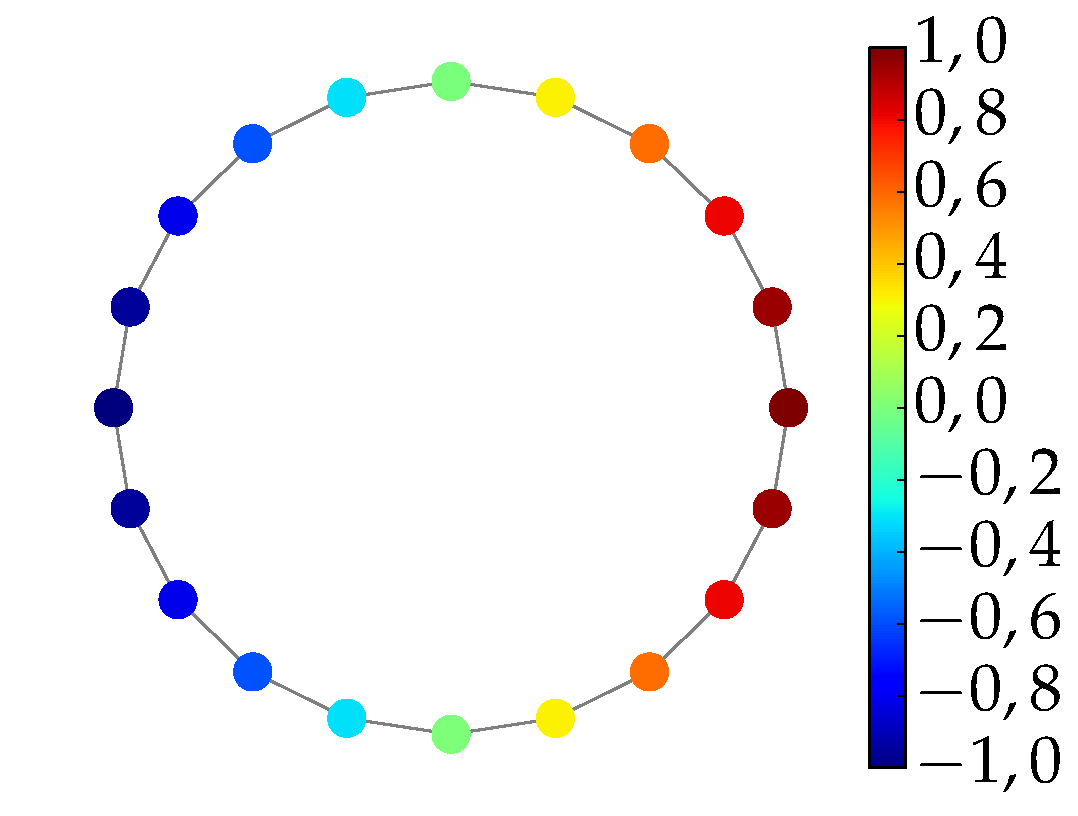
\includegraphics[width=\linewidth]{Figures/ring_different_structure_01_GSPA.pdf}
		}
	\end{minipage}~
	\begin{minipage}[c]{0.25\linewidth}
		\subfloat[\label{fig:diff_struct_b_GSPA}]{
			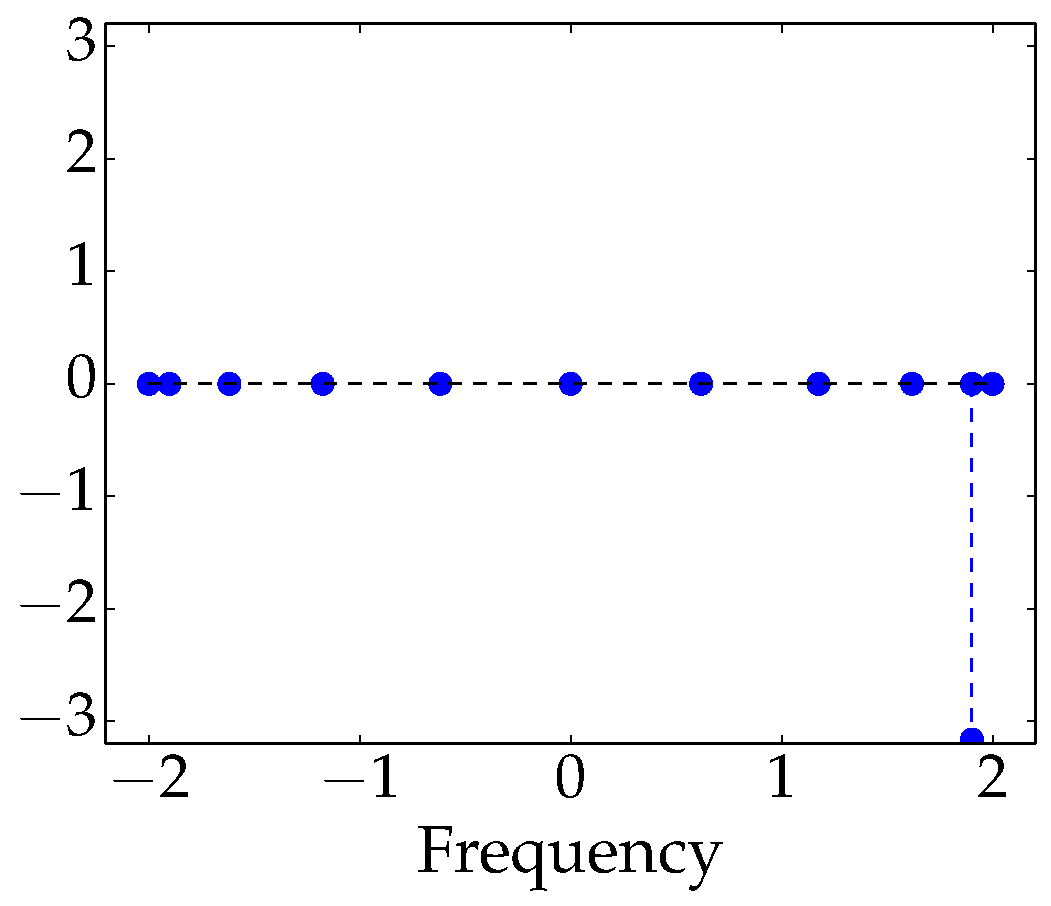
\includegraphics[width=\linewidth]{Figures/ring_different_structure_01_spectrum_GSPA_EN_2.pdf}
		}
	\end{minipage}%
	\floatsource
	\label{fig:diff_struct_GSPA}%
	\vspace{-0.2cm}
\end{figure}

The reader may have noticed a curious consequence from what was previously stated: unless the minimal and characteristic polynomials of $ \mathbf{A} $ are equal, the same frequency may be associated with two or more linearly independent frequency components, as indeed was the case in the example of Fig. \ref{fig:diff_struct_GSPA}. Furthermore, this figure shows that although the signal seems to be smooth, its frequency components are mostly associated with eigenvalues of high magnitude, what is counter-intuitive and provides a motivation to define a clear criterion to distinguish high and low graph frequencies.

The following mathematical reasoning consists of taking a metric which quantifies the expected signal smoothness, and use it to propose or confirm a notion of graph frequency. The metric used by Sandryhaila and Moura was the \emph{total variation}, taken from classical real analysis and defined for differentiable functions as \cite{rudin1987real,mallat1999wavelet}
\begin{equation}
%\label{key}
\Vert f \Vert_V = \int_{-\infty}^{\infty} |f'(t)| \mathrm{d}t.
\end{equation}

For discrete domain functions $ f_N[n] $, the Riemman integral is replaced by first order differences,
\begin{equation}
%\label{key}
\Vert f_N \Vert_V = \sum_p |f_N[n_p + 1] - f_N[n_p]|,
\end{equation}
which clearly quantifies the dissimilarity between contiguous values of the function $ f_N $. With this in mind, it was natural for Sandryhaila and Moura to use this metric in their attempt to quantify smoothness in GSP. Taking again the ring graph as a starting point, they looked at the total variation of a \textit{finite-length} discrete-time signal $ \mathbf{x} $:
\begin{equation}
\label{eq:TV}
TV(\mathbf{x}) = \sum_n | x_n - x_{(n-1) \text{ mod } N}|.
\end{equation}

From (\ref{eq:unit_shift}), one can see that (\ref{eq:TV}) may be written in terms of the $ \ell_1 $-norm\footnote{Throughout this text, the concepts of $ \ell_1 $- and $ \ell_2 $-norm will be frequently used. They are particular cases of the $ \ell_n $-norm of a vector $ \mathbf{x} \in \mathbb{C}^{N} $, defined as $ \Vert \mathbf{x}\Vert_n \overset{\Delta}{=} \left(\sum_{k=0}^{N-1} |x_k|^n\right)^{1/n} $.}
as $ TV(\mathbf{x}) = \Vert \mathbf{x} - \mathbf{C x}\Vert_1 $, by using the directed ring graph adjacency matrix to perform the cyclic shift. From that point, the generalization consisted of using this expression and defining the \emph{total variation on graphs} of a signal $ \mathbf{s} $ defined over the graph $ \mathcal{G} = \{\mathcal{V}, \mathbf{A}\} $ as
\begin{equation}
\label{eq:tv_graphs}
TV_G(\mathbf{s}) \overset{\Delta}{=} \Vert \mathbf{s} - \mathbf{A}^{\text{norm}} \mathbf{s}\Vert_1,
\end{equation}
with $ \mathbf{A}^{\text{norm}} = |\lambda_{max}|^{-1}\mathbf{A} $ and $ \lambda_{max} $ being the eigenvalue of $ \mathbf{A} $ having the highest absolute value. The normalization of the adjacency matrix aims to avoid the excessive magnification of the shifted signal \cite{sandryhaila2014frequency}.

\begin{figure}
	\centering
    \caption{Frequency ordering of graph signals, from low to high frequencies, in the complex plane.}
	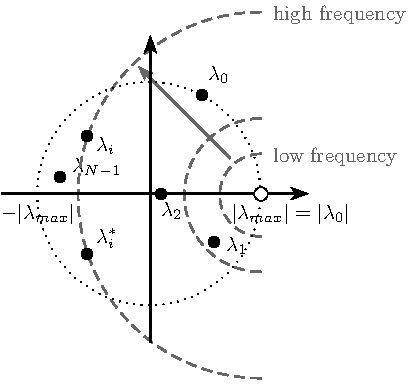
\includegraphics[width=0.45\linewidth]{Figures/graph_frequency_EN.pdf}
	\floatsource[adapted from \cite{sandryhaila2014frequency}]
	\label{fig:ordem_freq}
\end{figure}

Let $ \mathbf{A} $ be diagonalizable as in (\ref{eq:gft_01}) with (possibly complex) eigenvalues ordered like so
\begin{equation}
\label{eq:eig_order}
|\lambda_0| \leq |\lambda_1| \leq \dots \leq |\lambda_{N-1}| \overset{\Delta}{=} |\lambda_{max}|,
\end{equation}
associated with the eigenvectors $ (\mathbf{v}_i)_{i=0,\dots,N-1} $, scaled so that $ \Vert \mathbf{v}_i \Vert_1 = 1  \ \forall i$. Taking the total variation (on graphs) of the eigenvector $ \mathbf{v}_k $, one has
\begin{align*}
%\label{key}
TV_G(\mathbf{v}_k) &= \Vert \mathbf{v}_k - \mathbf{A} \mathbf{v}_k \Vert_1  = \Vert\mathbf{v}_k - \frac{1}{|\lambda_{max}|} \lambda_k \mathbf{v}_k \Vert_1 \notag \\
&= \left|1 - \frac{\lambda_k}{|\lambda_{max}|}\right| \Vert \mathbf{v}_k \Vert_1 = \Big| \lambda_k - |\lambda_{max}| \Big| \frac{\Vert \mathbf{v}_k \Vert_{1}}{|\lambda_{max}|}
\end{align*}
so that, since $ \Vert \mathbf{v}_k \Vert_1 = 1 $,
\begin{equation}
\label{eq:TV_ordering}
\Big| \! \lambda_i  - \! |\lambda_{max}|\Big| \! \leq \! \Big|  \lambda_j  - \! |\lambda_{max}|\Big| \! \! \iff \! \! TV_G(\mathbf{v}_i) \leq TV_G(\mathbf{v}_j),
\end{equation}
i.~e., frequency components associated with eigenvalues closer to the real point $ |\lambda_{max}| $ in the complex plane are \emph{smoother} (because they have lower total variation), and therefore are said to be of \emph{low frequency}. Fig. \ref{fig:ordem_freq} illustrates this ordering for graph frequencies, what clarifies the spectrum of the signal in Fig. \ref{fig:diff_struct_a_GSPA} (notice that since the graph is undirected, its adjacency matrix is symmetric and the eigenvalues are real-valued).


\begin{figure*}
	\centering
    \caption{(a) Directed sensor graph, with $ N=100 $ vertices and no loops or multiple edges. (b) Number of zero crossings and (b) total variation of the eigenvectors $ (\mathbf{v}_i)_{i=0,\dots,N-1} $ of the adjacency matrix $ \mathbf{A} $ of the graph in \emph{(a)}, ordered so that the respective eigenvalues appear from the closest to the farthest from the real point $ |\lambda_{max}| $ in the complex plane. That is, according to (\ref{eq:TV_ordering}) and Fig. \ref{fig:ordem_freq}, the eigenvectors are disposed in ascending order of frequency.}
	\subfloat[\label{fig:directed_graph}]{
			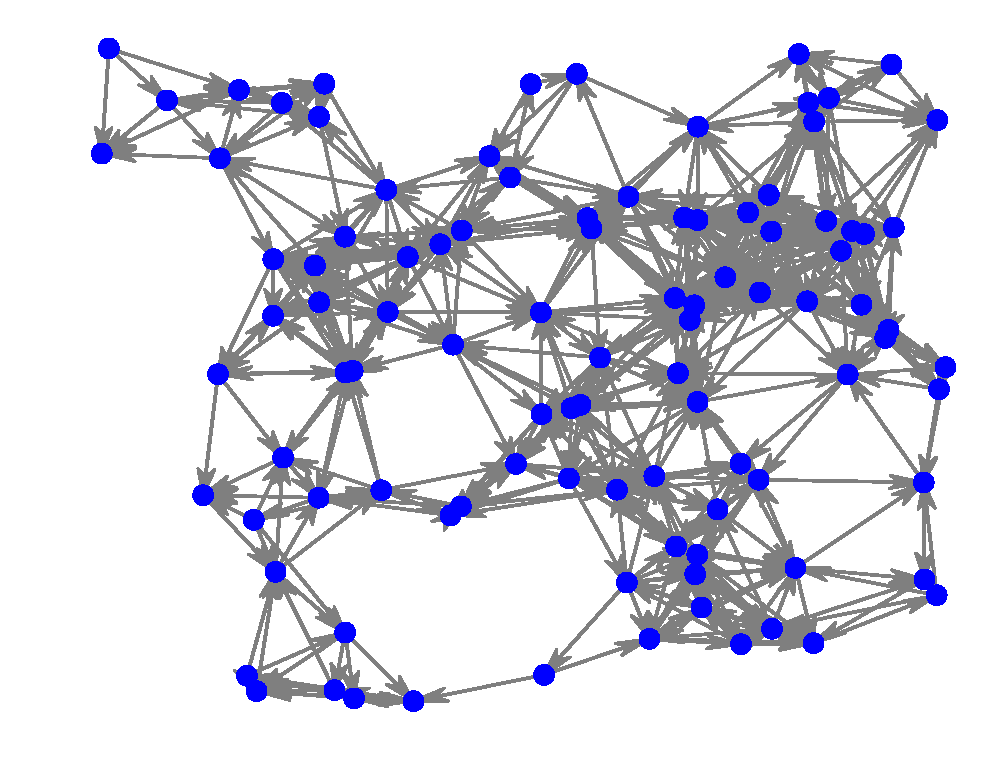
\includegraphics[width=0.31\linewidth]{Figures/showing_random_sensor_spectrum_directed_graph.pdf}
		}
	\subfloat[\label{fig:showing_random_sensor_spectrum_directed_b}]{
		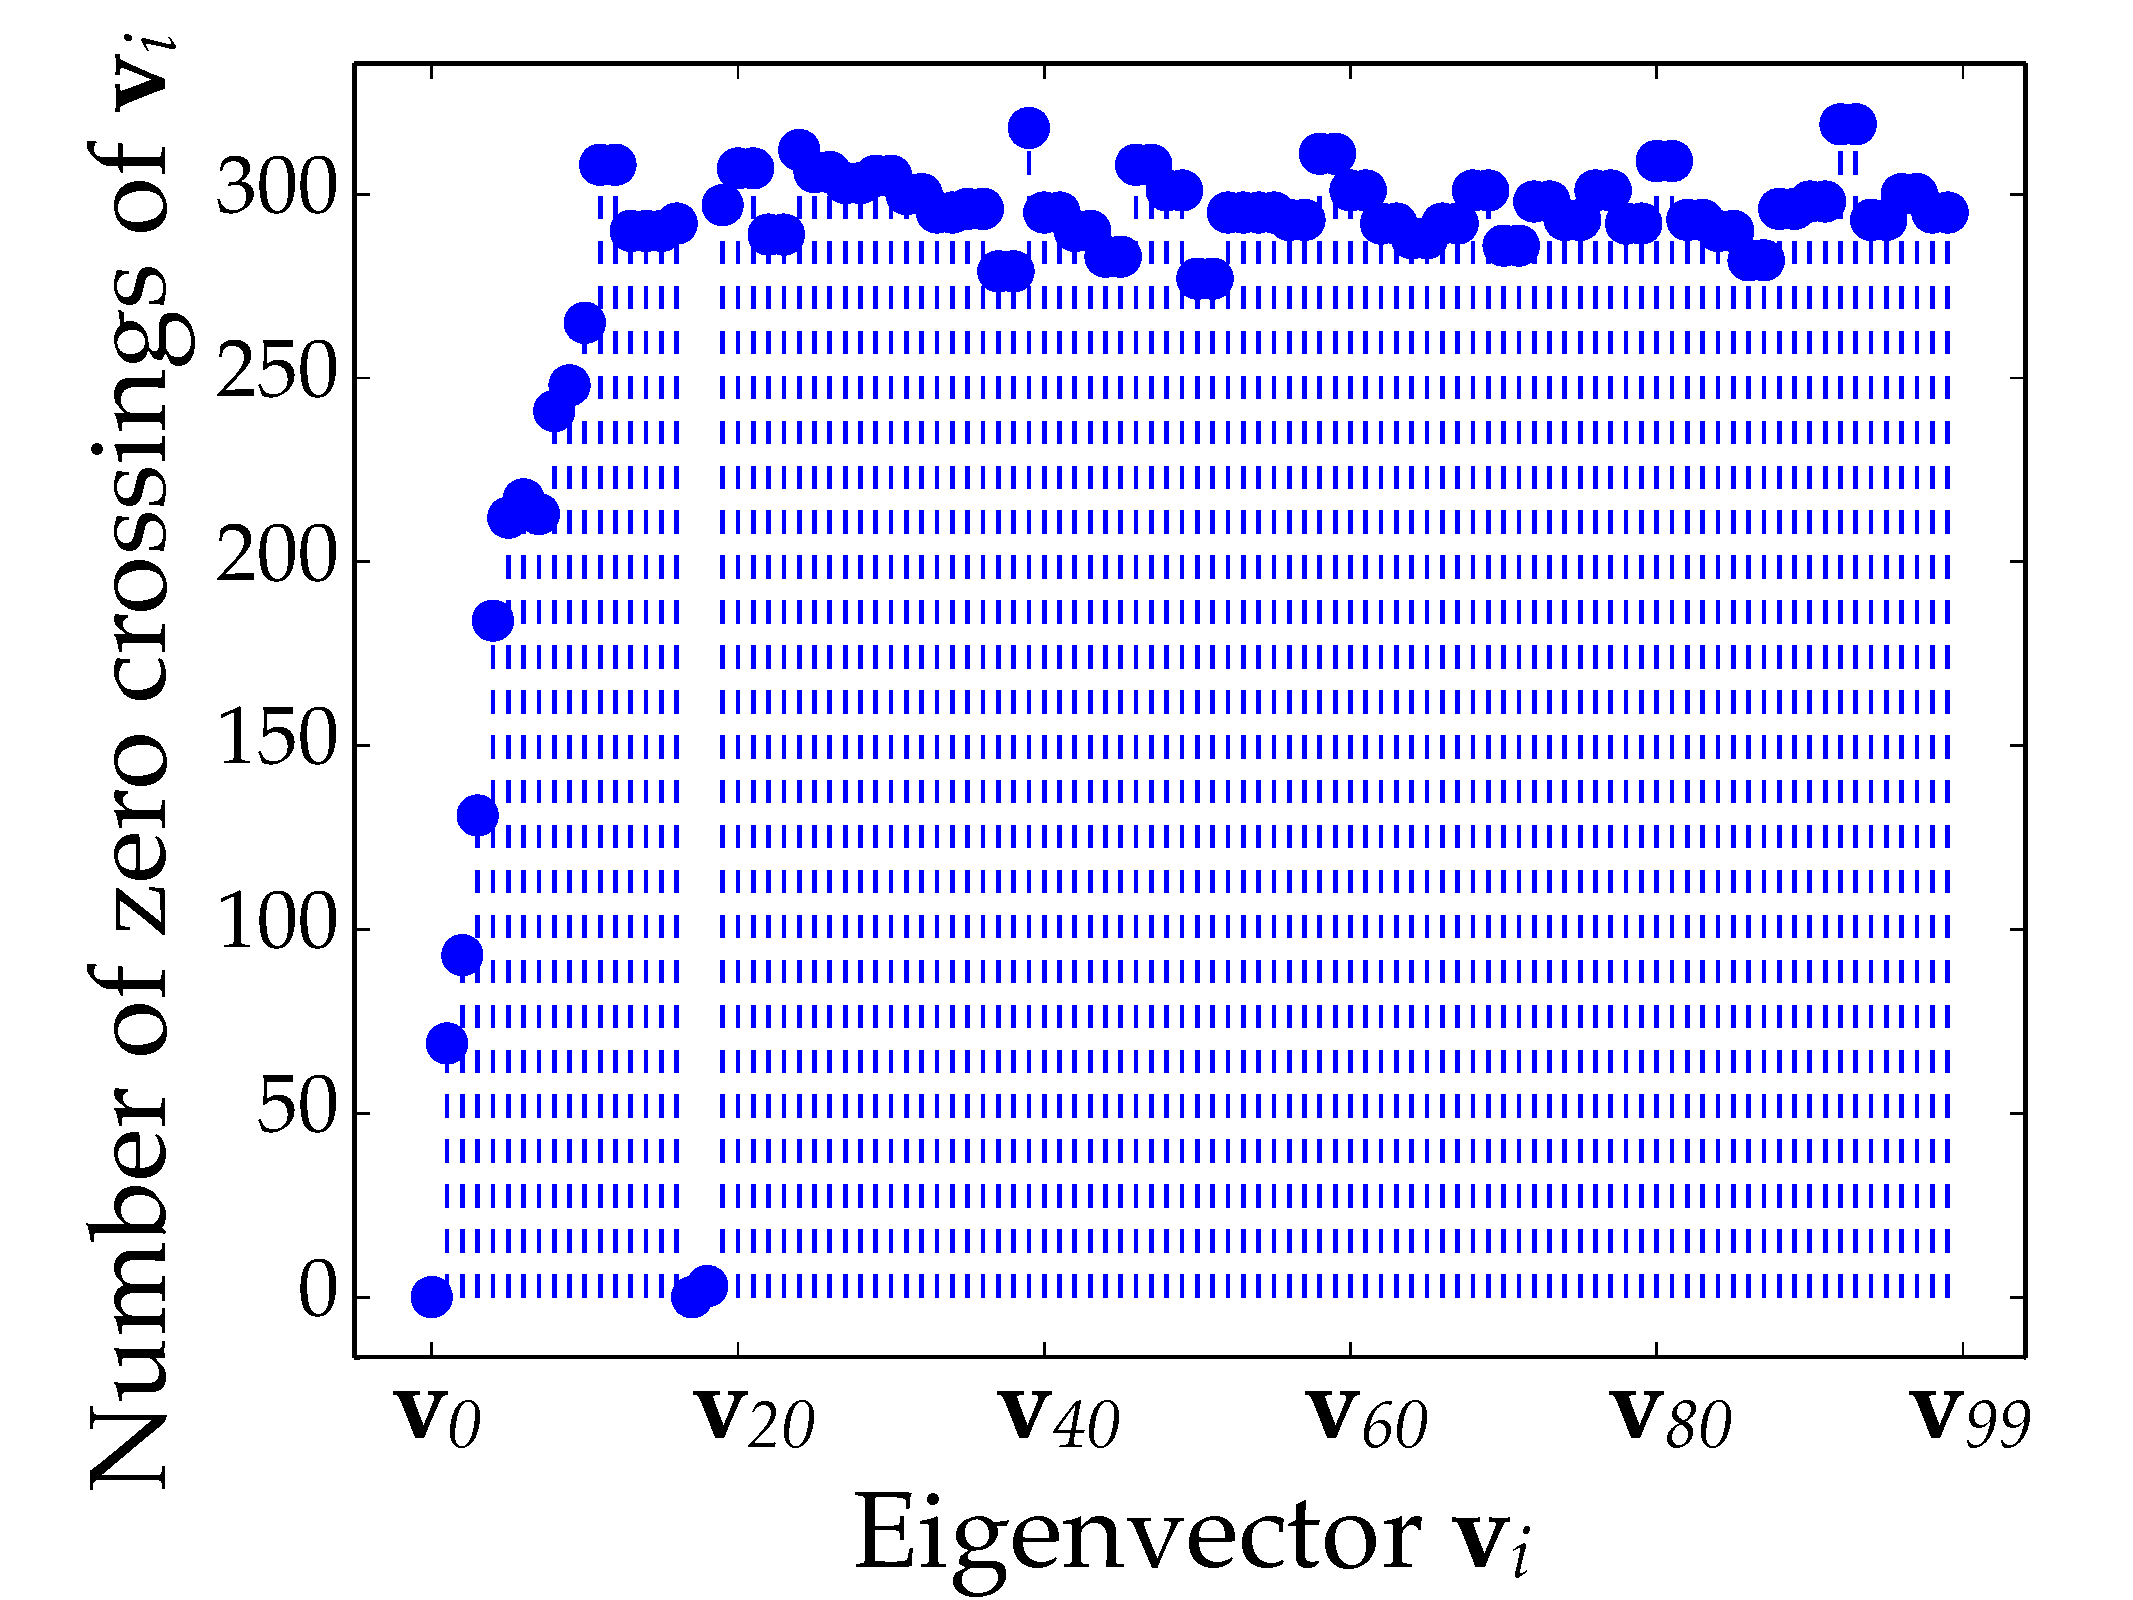
\includegraphics[width=0.33\linewidth]{Figures/showing_random_sensor_spectrum_directed_zero_crossings_1D_edited_EN.pdf}
	}~
	\subfloat[\label{fig:showing_random_sensor_spectrum_directed_c}]{
		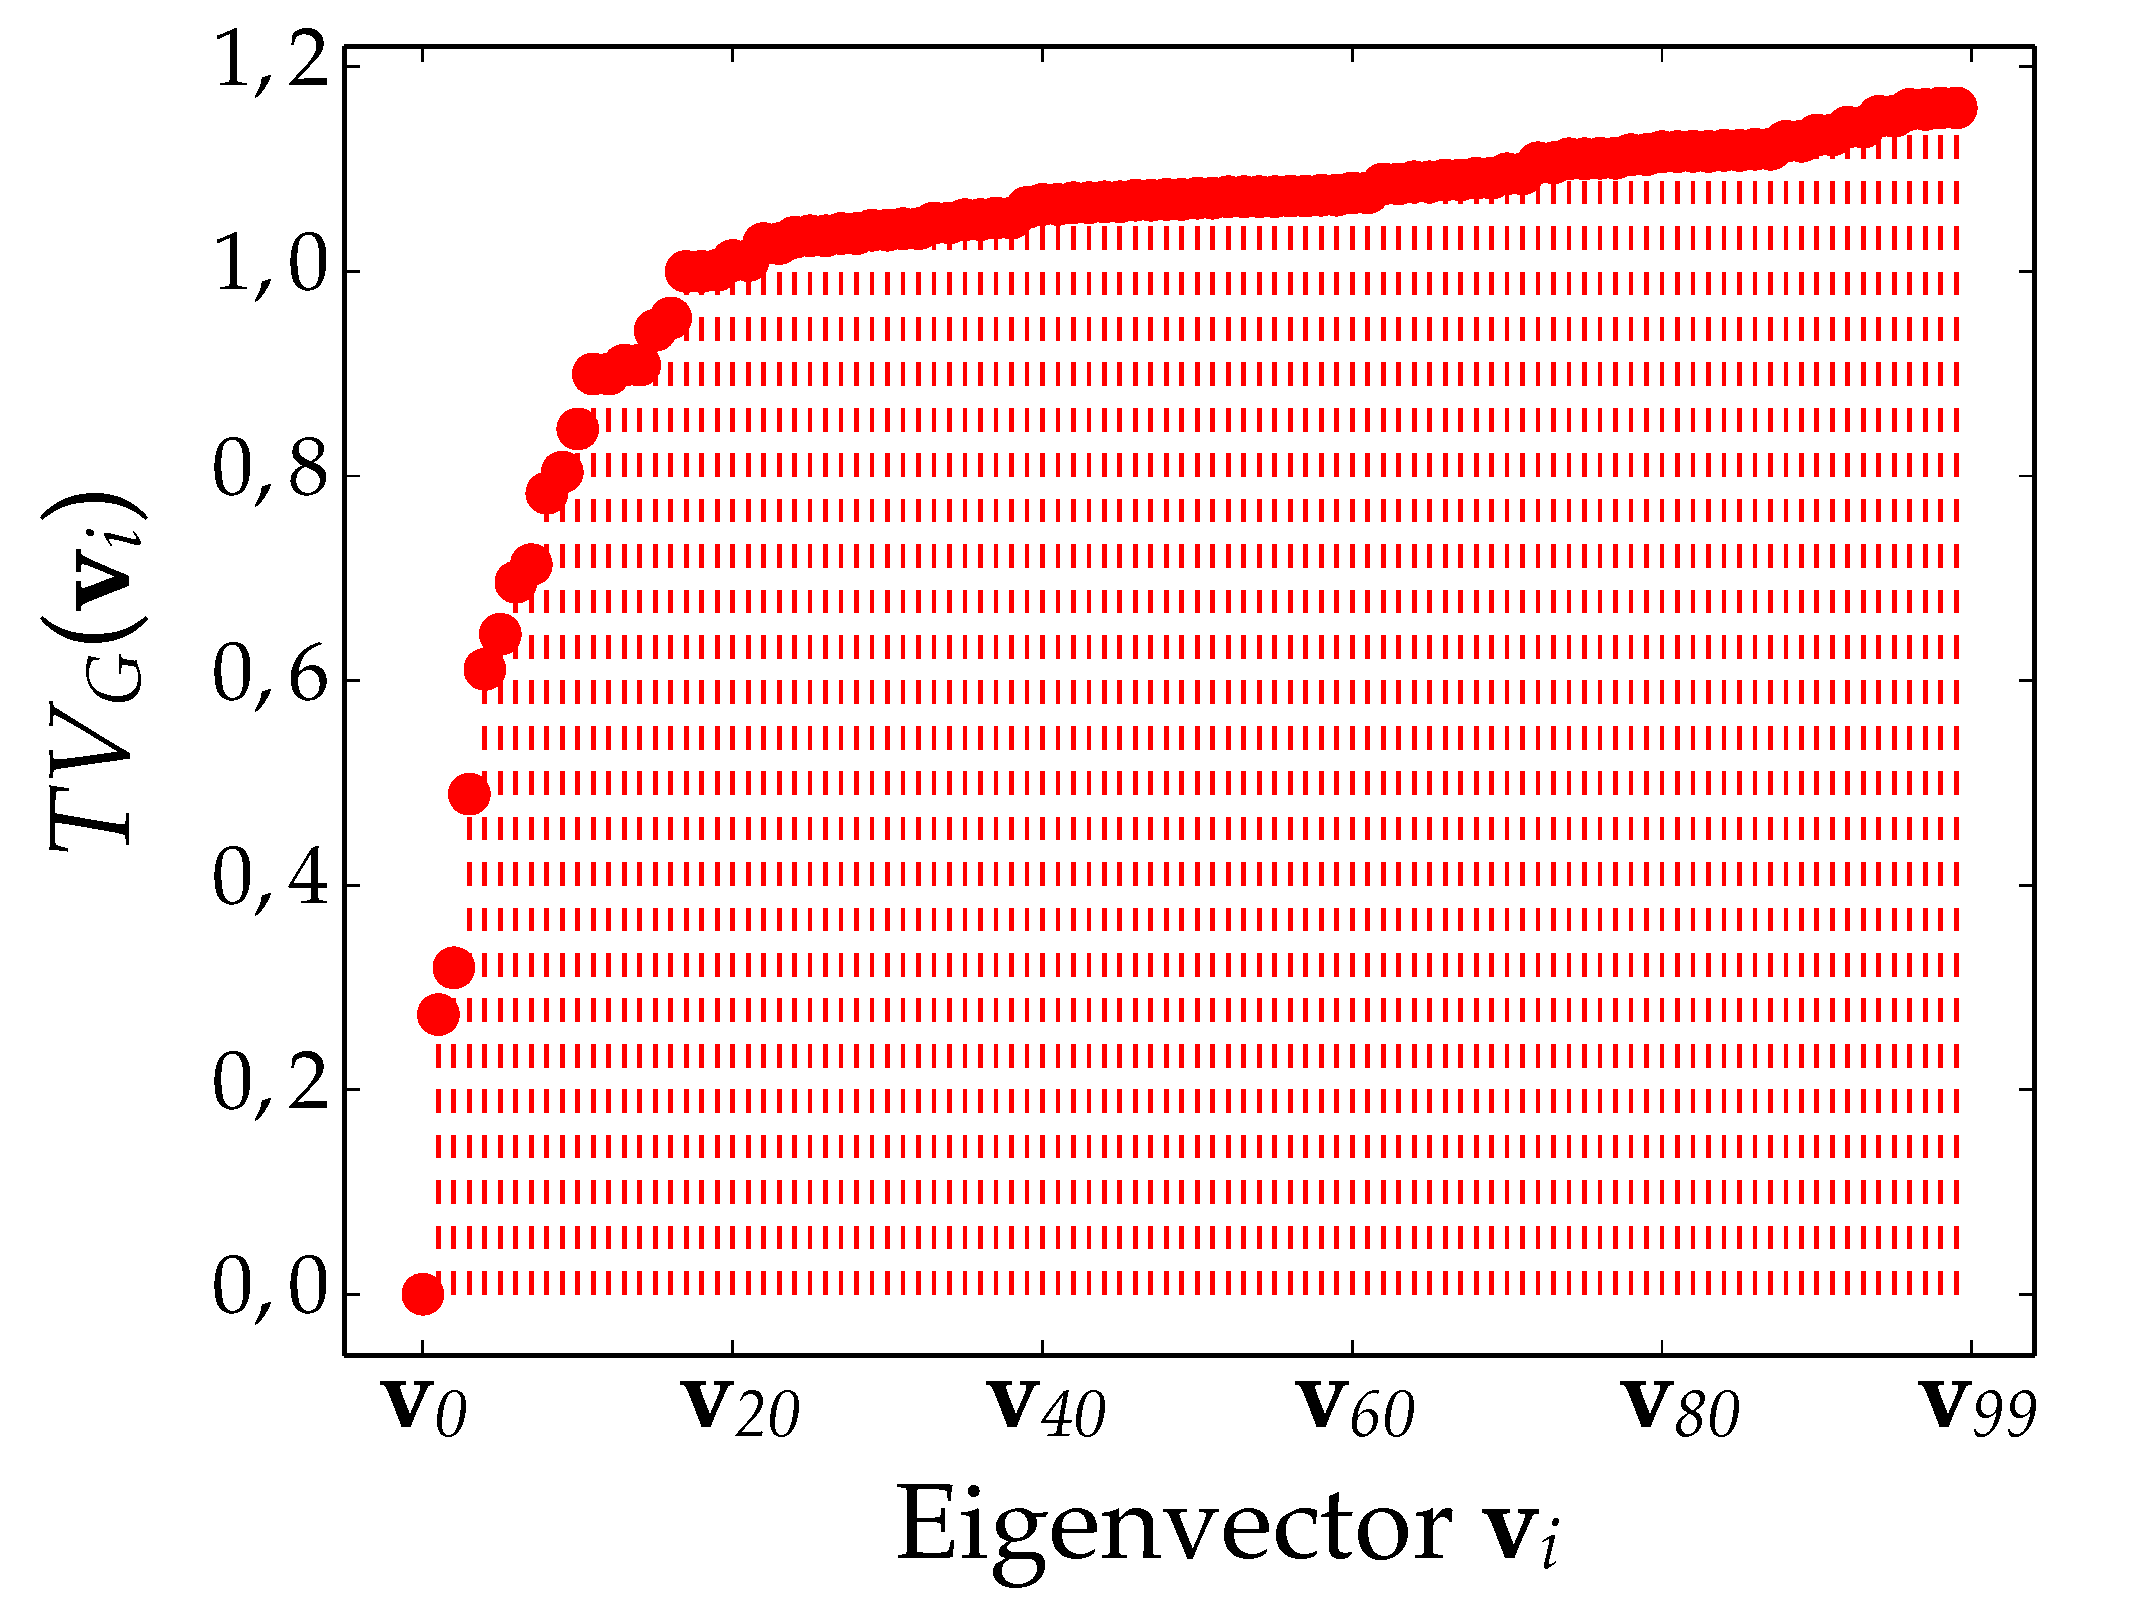
\includegraphics[width=0.33\linewidth]{Figures/showing_random_sensor_spectrum_directed_TV_1D_edited_EN.pdf}
	}
	\floatsource
	\label{fig:showing_random_sensor_spectrum_directed}
\end{figure*}

Let us take the directed graph in Fig. \ref{fig:directed_graph} to try to verify the consistency of the notion of frequency just derived. For this, along with the total variation on graphs, also the number of zero crossings (i.~e., the number of edges connecting vertices with signal samples of different sign) will be used to \emph{quantify} frequency. This quantity is also related to frequency in classical theory: the more a discrete signal has contiguous samples with different sign, generally the higher are its frequency components. These two functions, the total variation on graphs and the number of zero crossings, were calculated for each of the adjacency matrix eigenvectors, and the result is shown in Fig. \ref{fig:showing_random_sensor_spectrum_directed}, in which the eigenvectors $ \mathbf{v}_k $ are ordered in such a way that the respective eigenvalues $ \lambda_k $ appear from the closest to the farthest from the real point $ |\lambda_{max}| $ in the complex plane. Both metrics have similar behaviour, but since the number of zero crossings is indifferent to graph signal variations which do not change sign, it was already expected to be less accurate as a figure of merit for frequency. It matters to highlight, however, how the adopted eigenvector ordering indeed implies an ascending frequency order, since both functions in Fig. \ref{fig:showing_random_sensor_spectrum_directed_b} and \ref{fig:showing_random_sensor_spectrum_directed_c} agree on the tendency of growth. More than that, $ TV_G(\mathbf{v}_k) $ grows \emph{monotonically}, as it should do according to (\ref{eq:TV_ordering}).

It is convenient to conclude this discussion on the graph frequency domain by referring to the frequency response of graph filters. The definition given in Subsection \ref{subsec:filtros} considers the action of a matrix on a signal $ \mathbf{x} $ in the vertex domain of the graph $ \mathcal{G} = \{\mathcal{V}, \mathbf{A}\} $. In order to understand how the filter acts in the GFT domain, hereinafter called frequency domain, one may use (\ref{eq:gft_01}) and the polynomial representation of LSI filters. Let us take the filter $ \mathbf{H} =\sum_{\ell=0}^{L} h_\ell \mathbf{A}^\ell $ and its output to the input $ \mathbf{x} $ given by
\begin{align}\label{eq:resposta_freq_01}
\mathbf{H} \mathbf{x} &= \sum_{\ell=0}^{L} h_\ell \mathbf{A}^\ell \mathbf{x} =
\sum_{\ell=0}^{L} h_\ell \left(\mathbf{V} \mathbf{\Lambda} \mathbf{V}^{-1}\right)^\ell \mathbf{x} \notag \\
&= \mathbf{V} \left(\sum_{\ell=0}^{L} h_\ell \mathbf{\Lambda}^\ell \right) \mathbf{V}^{-1} \mathbf{x}.
\end{align}

Taking the GFT of both sides of the last equation yields
\begin{equation}\label{eq:resposta_freq_02}
\mathbf{V}^{-1} \mathbf{H} \mathbf{x} =
h(\mathbf{\Lambda}) \widehat{\mathbf{x}},
\end{equation}
which indicates that left-multiplication by $ \mathbf{H} $ (action of the filter in the vertex domain) is equivalent to the left-multiplication, in the frequency domain, by the matrix $ h(\mathbf{\Lambda}) $. In other words, $ h(\mathbf{\Lambda}) $ represents the frequency response of $ \mathbf{H} $.

\section{Summary}

This chapter guided the reader through the aspects regarding the fractional Fourier transform and graph signal processing most relevant to this work, closing the review of literature needed to have enough context to grasp and critique the chapters of original contributions that lie ahead. The key points to keep in mind are that
\begin{itemize}[noitemsep]
\item the fractional Fourier transform performs a real-valued rotation in the time-frequency plane,
\item the graph signal processing framework extends the usual discrete time domain to any network modeled by a graph, and as a consequence key basic concepts such as a unit shift must be redefined in terms of a graph matrix, called the graph shift operator,
\item the graph Fourier transform is the projection of a graph signal (vector) onto the space of eigenvectors of the graph shift operator.
\end{itemize}
\chapter{The fractional graph shift operator and its applications}
\label{ch:FrGSO}

Over the last decade, theory and applications related to graph signal processing have been widely developed and attracted the attention of several scholars~\cite{ortega2018,richard2018,ribeiro2018}. The reader may recall from Chapter \ref{ch:reviewGSP} that GSP aims to extend concepts and operations of classical digital signal processing to scenarios in which the signals lie over irregular domains. Such scenarios include, for instance, sensors arbitrarily positioned in a geographic region and measuring some climatological variable, points of a three-dimensional cloud representing some virtual object and its attributes, people linked according to their interests and proximity relationships in a social network and so on~\cite{chen2014,zhang2014,benzi2016,weiyu2018,saad2018,jiang2021,gama2019,liu2019,zhang2020,ferreira2020,zhang2021,xiao2021,sun2021}.

Among the research fronts active in GSP, the one that investigates alternatives to the shift operators, employed as building blocks to describe graph signals and systems, deserves to be highlighted~\cite{girault2015translation,gavili2017,fan20191,fan2019,mollaebrahim2021,shafipour2018,shafipour2019}. {In fact, when the purpose is to consider linear operators in this context, any matrix can be chosen to play the role of elementary building block; multiplying a matrix by a graph signal represented as a vector produces another signal whose samples result from a linear combination of the samples of the original signal. In this scope,} the use of matrices other than the \textit{standard} adjacency matrix and the Laplacian for the mentioned purpose may {be more suitable in specific scenarios and to carry out specific (graph) signal processing tasks. Even when the focus is on designing other graph operators (e.g., the graph Fourier transform), the decision about which elementary operator to use has an impact on the expected results.}

    {Regarding the issue discussed in the last paragraph, some relevant works in the GSP literature can be mentioned. In~\cite{girault2015translation}, for example, the authors propose an isometric graph translation operator that is described in the spectral domain as a phase shifting operator; this operator shares key properties with the time shift and behaves reasonably in the vertex domain. In~\cite{gavili2017}, the authors define an energy-preserving shift operator that satisfy many properties similar to their counterparts in classical signal processing; the GSP framework based on the referred operator enables the signal analysis along a correlation structure defined by a graph shift manifold. In~\cite{fan20191} and~\cite{fan2019}, the authors employ different features associated with a graph to generate a series of shift operators and design a graph-filter-based classifier. Although the proposed method produces better results than those achieved using conventional graph-filter-based classifiers, it requires dealing with a non-convex optimization problem whose solution involves a relatively high computational cost. In~\cite{mollaebrahim2021}, motivated by the typical scenario of asymmetric communications in wireless sensor networks, the authors study the optimal design of graph shift operators to perform decentralized subspace projection for asymmetric topologies. Obtaining the referred operators can be performed either by solving an optimization problem or by employing a decentralized algorithm based on an Alternating Direction Method of Multipliers (ADMM). In~\cite{shafipour2018} and~\cite{shafipour2019}, the goal is to construct a graph Fourier transform for directed graphs (digraphs), such that the corresponding orthonormal frequency components are as spread as possible in the graph spectral domain. The method uses the Laplacian of an undirected version of the digraph and involves non-convex, orthonormality-constrained optimization problems.}

    {This chapter brings contributions related to the above mentioned works by discussing the} possibility (and potentially useful consequences) of {computing} a non-integer power $\mathbf{A}^a$, $a\in\mathbb{R}$, of the adjacency matrix $\mathbf{A}$, {which is taken as} the (unit) graph shift operator~\cite{sandryhaila2014big}. {As a consequence}, the notion of fractional shift (or delay) of signals on graphs is presented, {which, to the best of the author's knowledge, has not yet been addressed in the literature. Differently from the referred papers, in which new operators are created or standard operators are adjusted using strategies potentially expensive from the computational point of view, a relatively simple generalization is proposed, which fills a theoretical gap concerning the extension to the GSP framework of a well-established concept in the classical signal processing.}

This chapter contains mostly the content of the paper \cite{ribeiro2022fractional}, published on the IEEE Access journal, and presents the contributions listed below.
\vspace{-1em}
\begin{itemize}[noitemsep]
    \item The introduction of the fractional graph shift operator $\mathbf{A}^a$ and the discussion of its several aspects. More specifically, the demonstration that $\mathbf{A}^a$ can be computed by using the theory of matrix functions, considering the Jordan decomposition of $\mathbf{A}$.

    \item The demonstration that $\mathbf{A}^a$ acts as a graph filter, furthermore giving its frequency response and discussing issues related to fractionally shifting graph signals containing descontinuities (Gibbs phenomenon).

    \item An analogy between the proposed graph fractional operator and that considered in the classical discrete-time case; suggesting that, when a directed ring graph with $N$ vertices is considered, the response of the corresponding graph filter related to $\mathbf{A}^a$ converges to that of the classical fractional delay filter as $N$ grows.

    \item The determination of the polynomial representation of $\mathbf{A}^a$ and, with that, the demonstration that, for any graph, such an operator can be implemented as a linear and shift-invariant (LSI) graph filter.
\end{itemize}

This chapter is organized as follows. In Section~\ref{sec:fracshift}, it is introduced the concept of fractional shift on graphs and the main contributions are developed: the computation of $\mathbf{A}^a$ in Subsection~\ref{subsec:comp}, discussion of its interpretation in Subsection~\ref{subsec:interpret}, demonstration of its consistency with the ideal fractional delay filter in Subsection~\ref{subsec:consist} and determination of its polynomial representation in Subsection~\ref{subsec:poly}. Section~\ref{sec:num} is devoted to numerical results related to the developed theory: it is firstly presented a small example regarding the polynomial representation of $\mathbf{A}^a$ in Subsection~\ref{subsec:num1}; then a real-world graph signal is considered (temperature measured by weather stations) and it is demonstrated that, using $\mathbf{A}^a$, one can obtain filters that approximate an ideal filter (in the least-squares sense) better than those designed using $\mathbf{A}$ (Subsections~\ref{subsec:lsi} and~\ref{subsec:lsi01}); finally, this possibility is illustrated by means of an example involving the noise removal from the same graph signal (Subsection~\ref{subsec:lsi02}). The chapter closes with concluding remarks in Section~\ref{sec:conc}.

\section{Fractional Shift on Graphs}\label{sec:fracshift}
Since the unit shift of a graph signal can be defined as the product by the adjacency matrix of the graph on which it lies, in this work, the proposed definition of a graph fractional shift as the product by a non-integer power of $ \mathbf{A} $. Precisely, the signal $\mathbf{x}$ over the graph $\mathcal{G} = \{ \mathbf{A}, {\mathcal{V}} \}$, after being shifted by $a\in[0,1]$, is given by
\begin{equation}
    \label{eq:def_frac_delay}
    \widetilde{\mathbf{x}}_a = \mathbf{A}^a \mathbf{x}.
\end{equation}
The following sections discuss aspects related to the computation of $\mathbf{A}^a$, the interpretation of its application to a graph signal and the consistency of the proposed operator with the classical DSP approach (ideal fractional delay filter).

\subsection{Computation of $\mathbf{A}^{{a}}$}\label{subsec:comp}
The computation of $\mathbf{A}^a$ can be well established by employing results from the theory of matrix functions~\cite{higham2008functions}. In this context, it suffices to evaluate the originally scalar function $f(t)=t^a$, $a\in\mathbb{R}$ having $\mathbf{A}$ as argument. The most direct way to formally define a function like this uses the Jordan canonical form. With this purpose, let us reconsider (\ref{eq:gft_01}), replacing the diagonalization of $\mathbf{A}$ with the most general decomposition
\begin{equation}
    \label{eq:Ajordan}
    \mathbf{A} = \mathbf{V} \mathbf{J} \mathbf{V}^{-1},
\end{equation}
using the Jordan block diagonal matrix $\mathbf{J}$,
\begin{equation}\label{eq:jcf}
    \mathbf{J}=\mathrm{diag}(\mathbf{J}_1,\mathbf{J}_2,\ldots,\mathbf{J}_p),
\end{equation}
and the matrix $\mathbf{V}$ of generalized eigenvectors. Each $k$-th Jordan block $\mathbf{J}_k$ is
\begin{equation}
    \mathbf{J}_k=\mathbf{J}_k(\lambda_k)=\left[\begin{array}{cccc}
            \lambda_k & 1         &        &           \\
                      & \lambda_k & \ddots &           \\
                      &           & \ddots & 1         \\
                      &           &        & \lambda_k
        \end{array}\right]\in\mathbb{C}^{m_k\times m_k}
\end{equation}
and $m_1+m_2+\ldots +m_p=N$. Denote by $\lambda_1,\ldots,\lambda_s$ the distinct eigenvalues of $\mathbf{A}$ and by $n_i$ the \emph{index} of $\lambda_i$ (the order of the largest Jordan block in which $\lambda_i$ appears). The function $f$ is said to be defined on the spectrum of $\mathbf{A}$ if the values
\begin{equation}\label{eq:defspec}
    f^{(j)}(\lambda_i),\quad j=0,1,\ldots,n_i-1,\quad i=1,2,\ldots,s,
\end{equation}
exist, where $f^{(j)}$ denotes the $j$-th derivative of $f$.\footnote{As usual, the notation $f'$ will be used interchangeably with $f^{(1)}$.} That holds true for $f(t)=t^a$. The computation of $f(\mathbf{A})=\mathbf{A}^a$ can then be carried out as follows.
\vspace{0.2cm}
\begin{definition}\label{def:jc01}
Let $f$ be defined on the spectrum of $\mathbf{A}\in\mathbb{C}^{N\times N}$ and let $\mathbf{A}$ have the Jordan decomposition~(\ref{eq:Ajordan}). Then
\begin{equation}\label{eq:jcf01}
f(\mathbf{A})\overset{\Delta}{=}\mathbf{V}f(\mathbf{J})\mathbf{V}^{-1}=\mathbf{V} \ \mathrm{diag}(f(\mathbf{J}_k)) \ \mathbf{V}^{-1},
\end{equation}
where
\begin{equation}\label{eq:jcf02}
f(\mathbf{J}_k)\overset{\Delta}{=}\left[\begin{array}{cccc}
f(\lambda_k) & f'(\lambda_k) & \cdots & \frac{f^{(m_k-1)}(\lambda_k)}{(m_k-1)!} \\
& f(\lambda_k)  & \ddots & \vdots                                  \\
&               & \ddots & f'(\lambda_k)                           \\
&               &        & f(\lambda_k)\end{array}\right]
\end{equation}
and $\mathrm{diag}(\cdot)$ is intended to represent a block-diagonal matrix constituted using the blocks $f(\mathbf{J}_k)$.
\end{definition}
In the present context, the last definition constitutes a practical way to calculate $\mathbf{A}^a$, because the Jordan form of the adjacency matrix, being necessary for the definition of the corresponding GFT, may already have been computed and thus be available to be used in~(\ref{eq:jcf01}) and~(\ref{eq:jcf02}).


\subsection{Interpreting the graph fractional shift}\label{subsec:interpret}
In order to perform a meaningful interpretation of the graph fractional shift, we consider~(\ref{eq:def_frac_delay}) and the case in which $\mathbf{A}$ is diagonalizable. Using the matrix factorization~(\ref{eq:gft_01}), the GFT analysis equation~(\ref{eq:GFT_fwd}) and the computation strategy described in the last subsection, we can write
\begin{align}\label{eq:frac_delay_01}
    \mathbf{A}^a \mathbf{x} & = \mathbf{V} \mathbf{\Lambda}^a \mathbf{V}^{-1} \mathbf{x} = \mathbf{V}
    \begin{bmatrix}
        \lambda_1^a &        &             \\
                    & \ddots &             \\
                    &        & \lambda_N^a
    \end{bmatrix}
    \widehat{\mathbf{x}} \notag                                                                                                                                         \\[0.5em]
                            & = \mathbf{V} (\widehat{\mathbf{h}}_a \odot \widehat{\mathbf{x}}) = \text{GFT}^{-1} \{\widehat{\mathbf{h}}_a \odot \widehat{\mathbf{x}}\},
\end{align}
where $\widehat{\mathbf{h}}_a \overset{\Delta}{=} (\lambda_1^a \ \ldots \ \lambda_N^a)^T$ and $\odot$ represents the point-wise vector product.

Equation~(\ref{eq:frac_delay_01}) shows that $ \mathbf{A}^a $ is a graph filter with frequency response $ \mathrm{diag}(\widehat{\mathbf{h}}_a) $; moreover, if $ \mathbf{x} $ is an $N$-point discrete-time signal (case in which the GFT coincides with the DFT), one observes that the filter in the DFT domain is the vector $ \widehat{\mathbf{h}}_a $ itself. In this case, it has been discussed that the adjacency matrix of the respective graph is diagonalized according with~(\ref{eq:diag_C}), where $ \mathbf{\Lambda}_{\mathbf{C}} $ has as entries the $ N $ roots of unity. The fact that the matrix of eigenvectors of $ \mathbf{C} $ is the Fourier matrix imposes a specific order of the eigenvalues in $ \mathbf{\Lambda}_{\mathbf{C}} $, so that the vector $ \widehat{\mathbf{h}}_a$ is
\begin{align*}
    \widehat{\mathbf{h}}_a & = (1 \,\, W_N^a \,\,W_N^{2a}\ldots W_N^{aR} \,\,W_N^{-aR'} \,\,W_N^{a(-R' + 1)}\ldots W_N^{-a}),
\end{align*}
where $ W_N = e^{-j \frac{2\pi}{N}} $ and
\begin{equation}
    \begin{cases}
        R = \frac{N-1}{2} \text{ and } R' = R,     & \text{ if } N \text{ is odd},\vspace{0.2cm} \\
        R = \frac{N}{2} - 1 \text{ and } R' = R+1, & \text{ if } N \text{ is even},
    \end{cases}
\end{equation}
$n=0,1,\ldots,N-1$. It can be shown that the inverse DFT of $ \widehat{\mathbf{h}}_a $ has components given by~(\ref{eq:DFT_inversa_autovalores}).

\begin{figure*}%[h!]
\begin{equation}\label{eq:DFT_inversa_autovalores}
h_a[n]\hspace{-0.03cm}=\hspace{-0.03cm}
\left\{\begin{array}{ll}
    %\displaystyle
    {\dfrac{1}{N}} \dfrac{\sin (\pi (n-a))}{\sin \left(\frac{\pi}{N} (n-a)\right)},                             & \text{ if $N$ is odd},\vspace{0.25cm} \\
    %\displaystyle
    {\dfrac{1}{N} \cot \left(\dfrac{\pi}{N} (n-a)\right) \sin (\pi (n-a))}{+ \dfrac{j}{N} (-1)^n \sin (\pi a)}, & \text{ if } N \text{ is even}.
\end{array}\right.
\end{equation}
% \hrule
\end{figure*}

\begin{figure}[b]
    \centering
    \caption{Fractional shift by $a=0{.}3 $ of a sample of a signal on a directed ring graph with unit weights. (a) Original signal on a directed ring graph. (b) Graph in which the 5$\textsuperscript{th}$ sample delayed by $a=0{.}3 $ appears as an interpolated sample between the 4$\textsuperscript{th}$ and the 5$\textsuperscript{th}$ samples of the original signal. (c) Original discrete signal and the delayed sample.}
    \subfloat[\label{figa_frac_delay_directed}]{{
                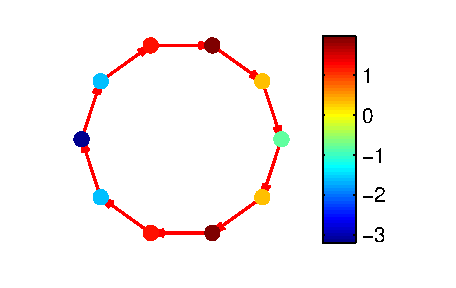
\includegraphics[width=0.35\linewidth]{Figures/d170309_frac_delay_ring_visualization_V5_a.eps}
            }}
    %	\vspace{-0.2cm}
    \subfloat[\label{figb_frac_delay_directed}]{{
                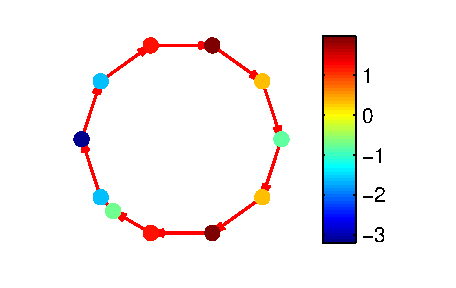
\includegraphics[width=0.35\linewidth]{Figures/d170309_frac_delay_ring_visualization_V5_b.eps}
            }}\\
    \subfloat[\label{figc_frac_delay_directed}]{{
                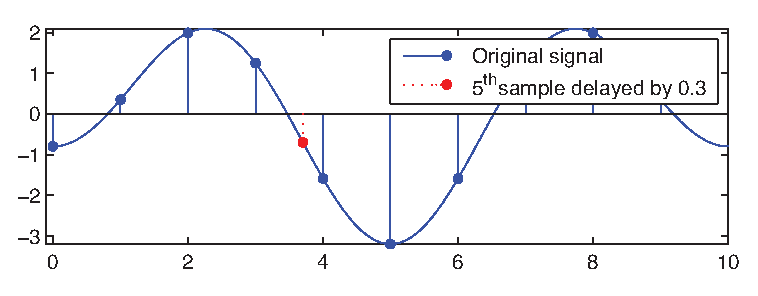
\includegraphics[width=0.6\linewidth]{Figures/d170309_frac_delay_ring_visualization_V5_c1.eps}
            }}% 
    \floatsource
    \label{fig:frac_delay_directed}
    %\vspace{-0.3cm}
\end{figure}

The product by a fractional power of the adjacency matrix produces the effect illustrated in Fig. \ref{fig:frac_delay_directed}, for a directed ring graph; it can be seen, for example, how the 5\textsuperscript{th} sample of the signal shifted by $a=0{.}3 $ coincides with the value of the continuous-time signal at the same position. On the other hand, the analysis we can perform by observing the \textit{irregular} graph in Fig.~\ref{fig:sinal_Pernambuco} is mostly visual; as we vary the fractional parameter from $0$ (original signal) to $1$, we see in the intermediate snapshots how the signal gradually spreads out from the vertices where, originally, there were already non-zero samples. In this scope, although we employ terms such as delay and shift, which are inherited from classical signal processing, the process observed in the figure looks more like a kind of (fractional) diffusion. In fact, diffusion on graphs have been widely studied~\cite{zhang2008,thanou2017, benzi2021}; it is usually described in terms of a system of ordinary differential equations in time, with the Laplacian matrix of the graph as the coefficient matrix. Fractional diffusion has been used to model certain phenomena that allow long-range interactions and are non-local in nature~\cite{ilic2005,riascos2014,estrada2021,antil2021}.

Finally, it matters to highlight the fact that the signal to be shifted has to be bandlimited (see Fig.~\ref{figa_gibbs}). If the signal has abrupt changes in its sample values, this can be viewed as a kind of descontinuity and represents high frequency components, when compared to the predominantly smooth behavior of the signal (see Fig.~\ref{figb_gibbs}). As a consequence, we can observe considerable fluctuations around the disparate samples when the signal is fractionally delayed, an effect similar to the Gibbs phenomenon.

\begin{figure}[t!]
    \centering
    \caption{Fractional shift of a signal, (originally) with $10$ non-zero samples, defined on a graph formed by $80$ cities of Pernambuco state, Brazil. Note that the shifted signal is similar to the original signal, if $ a $ is close to $0$, and similar to the unit-shifted signal, if $ a $ is close to $1$.}%
    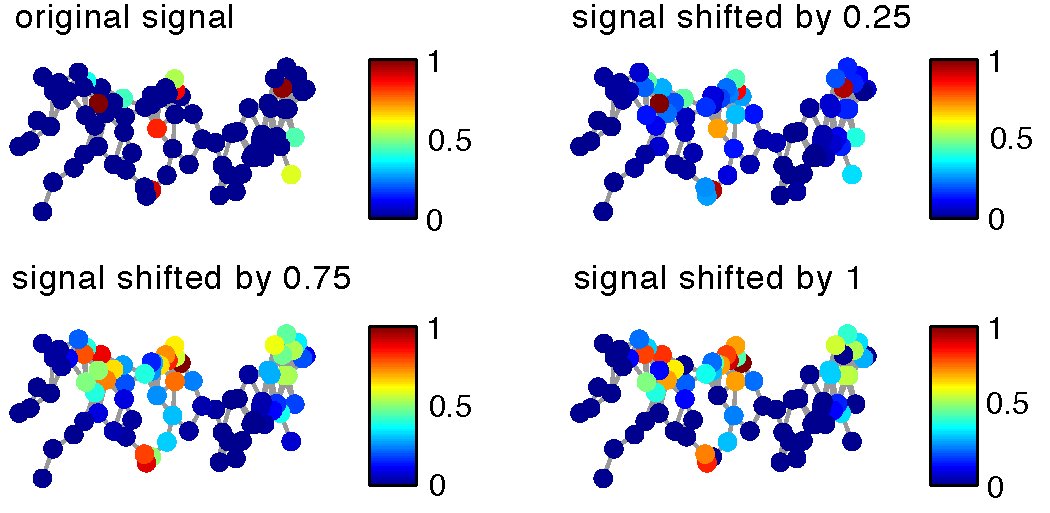
\includegraphics[width=0.6\linewidth]{Figures/signal_PE_V2_PT.pdf}
    \floatsource
    \label{fig:sinal_Pernambuco}%
    \vspace{-0.2cm}
\end{figure}

\begin{figure}[t!]
    \centering
    \caption{Fractional shift for a signal (a) without and (b) with abrupt variations (descontinuities).}%
    \subfloat[\label{figa_gibbs}]{{
                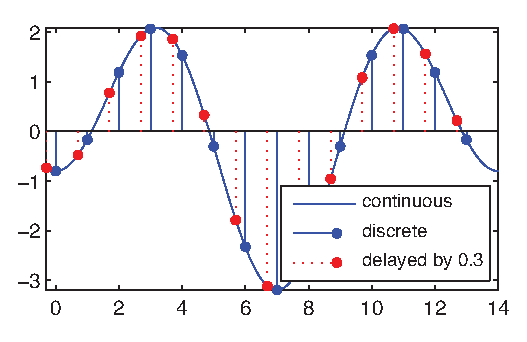
\includegraphics[width=0.4\linewidth]{Figures/d170309_frac_delay_ring_visualization_V2_no_gibbs.eps}
            }}~
    %	\vspace{-0.2cm}
    \subfloat[\label{figb_gibbs}]{{
                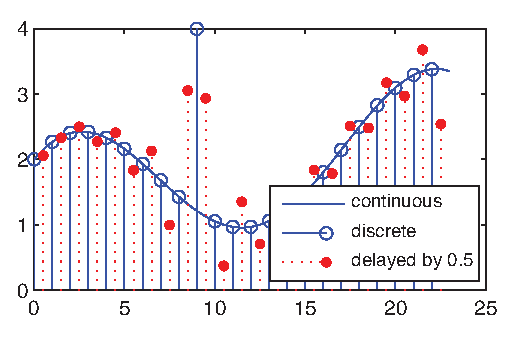
\includegraphics[width=0.4\linewidth]{Figures/frac_delay_ring_TESTS_gibbs_effect.eps}
            }}%
    \floatsource
    \label{fig:frac_delay_gibbs}%
    \vspace{-0.2cm}
\end{figure}

\subsection{Consistency with classical approach: the ideal fractional delay filter}\label{subsec:consist}
In the classical approach to the problem of fractionally shifting a discrete-time signal, the continuous-time version of the signal can be reconstructed, shifted and then resampled with the same sampling period~\cite{alan1989discrete,valimaki1995discrete}. Due to the Nyquist-Shannon Theorem, this procedure requires that the signal is bandlimited. In this context, it can be shown that, if a discrete-time signal $ \mathbf{x} $ is bandlimited, its version shifted by $ a \in [0,1] $ is
$$
    x[n-a] = \sum_k x[k] \mathrm{sinc} (n - k - a),
$$
so that the (ideal low-pass) filter used to perform the referred shift has components
\begin{equation}
    h_{_{LPF}}[n] = \mathrm{sinc} (n-a).
\end{equation}

The filter $ \mathbf{h}_{_{LPF}} $ is non-causal and unstable (it is not BIBO -- \emph{bounded input, bounded output}, because its impulse response has infinite energy) and, therefore, it is not physically realizable. In this way, fractional delay filter implementations should just \emph{approximate} $ \mathbf{h}_{_{LPF}} $ as much as possible.

In order to evaluate how close to $ h_{_{LPF}}[n] = \mathrm{sinc} (n-a) $, $ 0\leq a \leq 1 $, is $h_a[n]$, for odd $N$ (see the first row of~(\ref{eq:DFT_inversa_autovalores})), the point-wise difference between these signals has been computed for different values of $ N \in [10^1, 10^6]$. Fig. \ref{fig:convergence}, shows the relative error (ratio between the energy of the error $(\mathbf{h}_a - \mathbf{h}_{_{LPF}})$ and that of $ \mathbf{h}_{_{LPF}} $), in terms of $ N $ and $a $.

The result suggests that, in fact, $ \mathbf{h}_a $ converges in the mean in $ \ell^2 $ to $ \mathbf{h}_{_{LPF}}$ as $ N $ grows, with relative error less than $ 5\% $ for $ N \approx 30 $. Moreover, the error is greater when $ a $ is close to $ 0{.}5 $, being negligible or null when $ a $ is an integer. In fact, the error is exactly zero for $ a=0$ (or $a=1$) and $ n = a $, since
\begin{equation}\label{eq:lim_h_impar}
    \lim_{n \rightarrow a} h_{a}[n] = 1
    \Rightarrow
    \lim_{n \rightarrow a} \big(h_{a}[n] - \mathrm{sinc}(n-a)\big) = 0.
\end{equation}

The same result is obtained for even $N$, starting from the second row of~(\ref{eq:DFT_inversa_autovalores}). When $a$ is non-integer, $h_a[n] $ is complex, with imaginary part of constant modulus for a fixed $a$. Considering the corresponding real part only, the error was smaller than that taking into account also the contribution of the imaginary part. Fig. \ref{fig:convergence_even_N_real_part} and Fig. \ref{fig:convergence_even_N_abs} show that the errors with and without the imaginary part equally decay as  $ N $ grows, but, using the real part only, the results are significantly better.

\begin{figure}[ht!]
    \centering
    \caption{Percent error (normalized by the energy of $ \mathbf{h}_{_{LPF}} $) of $ \mathbf{h}_a $ related to $ \mathbf{h}_{_{LPF}} $, for different (odd) values of $ N $ and the fractional shift parameter $ a $.}
    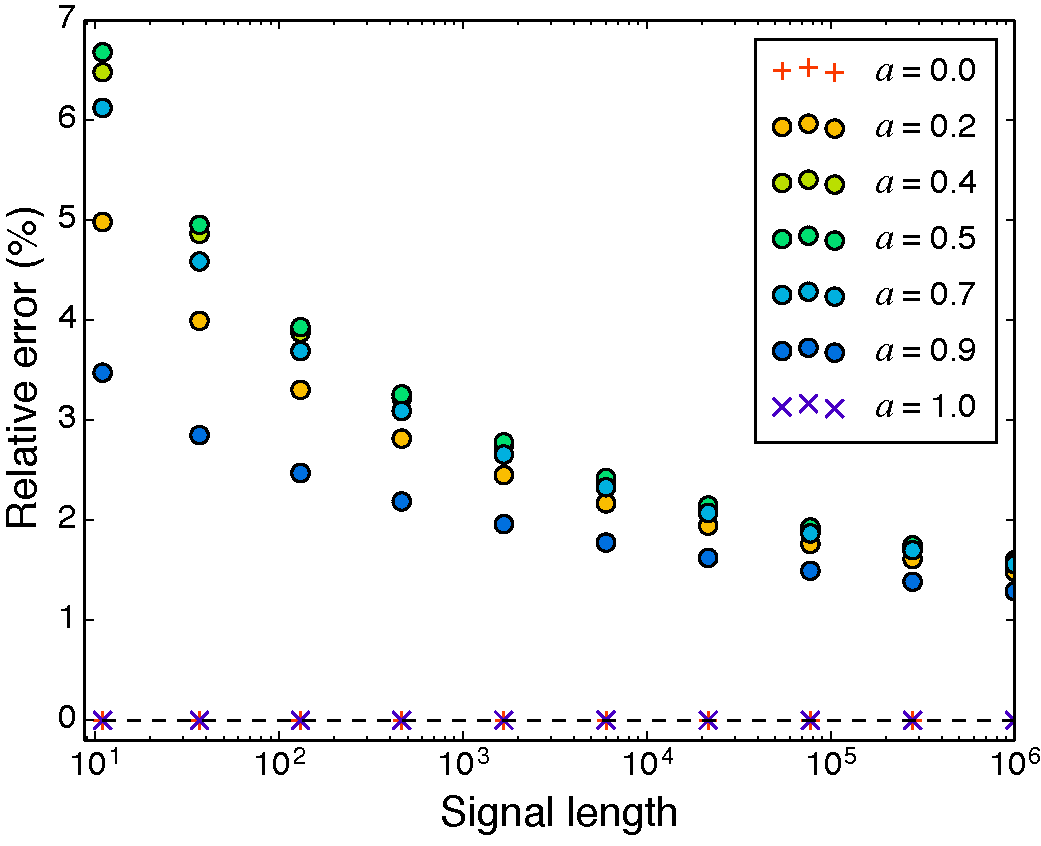
\includegraphics[width=0.5\linewidth]{Figures/convergence_odd_N_V4.pdf}
    \floatsource
    \label{fig:convergence}
\end{figure}

\begin{figure}[ht!]
    \centering
    \caption{Relative mean error between $ \mathcal{R}e\{\mathbf{h}_a\} $ and $ \mathbf{h}_{_{LPF}} $ for $ N $ even, in terms of the fractional shift parameter $a$.}
    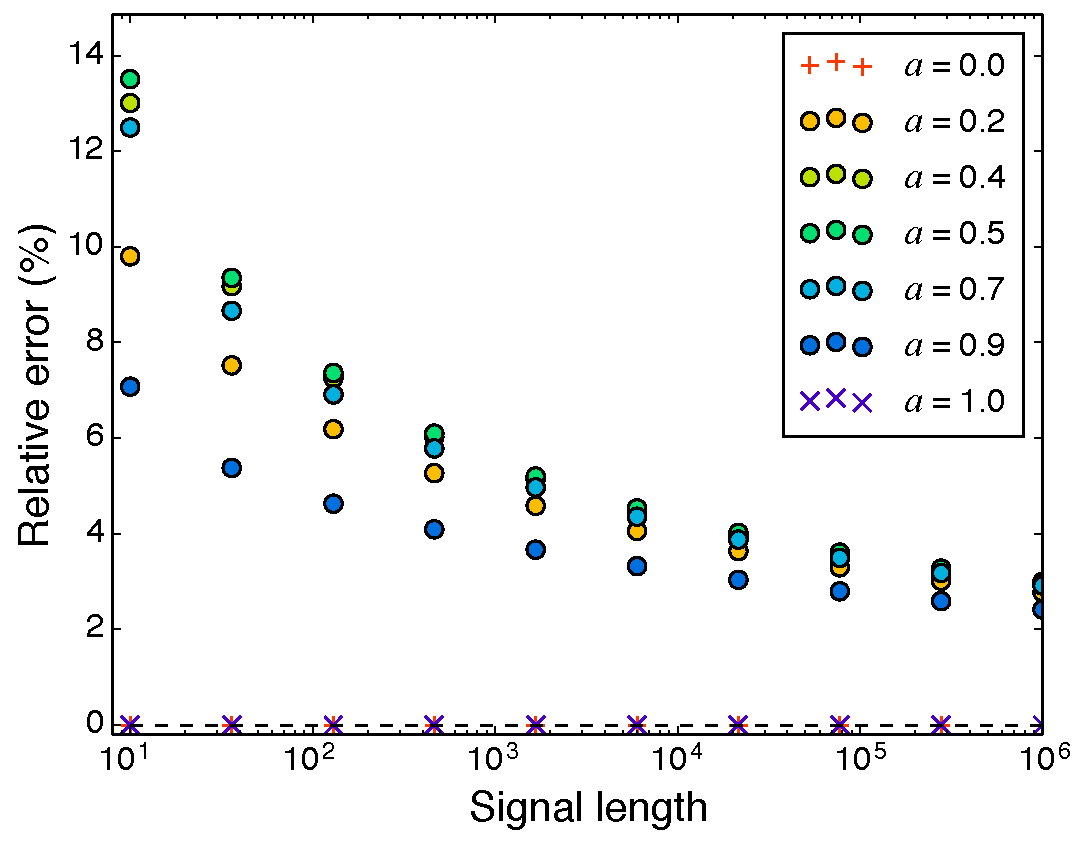
\includegraphics[width=0.5\linewidth]{Figures/convergence_even_N_real_part.pdf}
    \floatsource
    \label{fig:convergence_even_N_real_part}
\end{figure}

\begin{figure}[ht!]
    \centering
    \caption{Modulus of the relative mean error between $ \mathbf{h}_a $ and $ \mathbf{h}_{_{LPF}} $ for $ N $ even, in terms of the fractional shift parameter $a$.}
    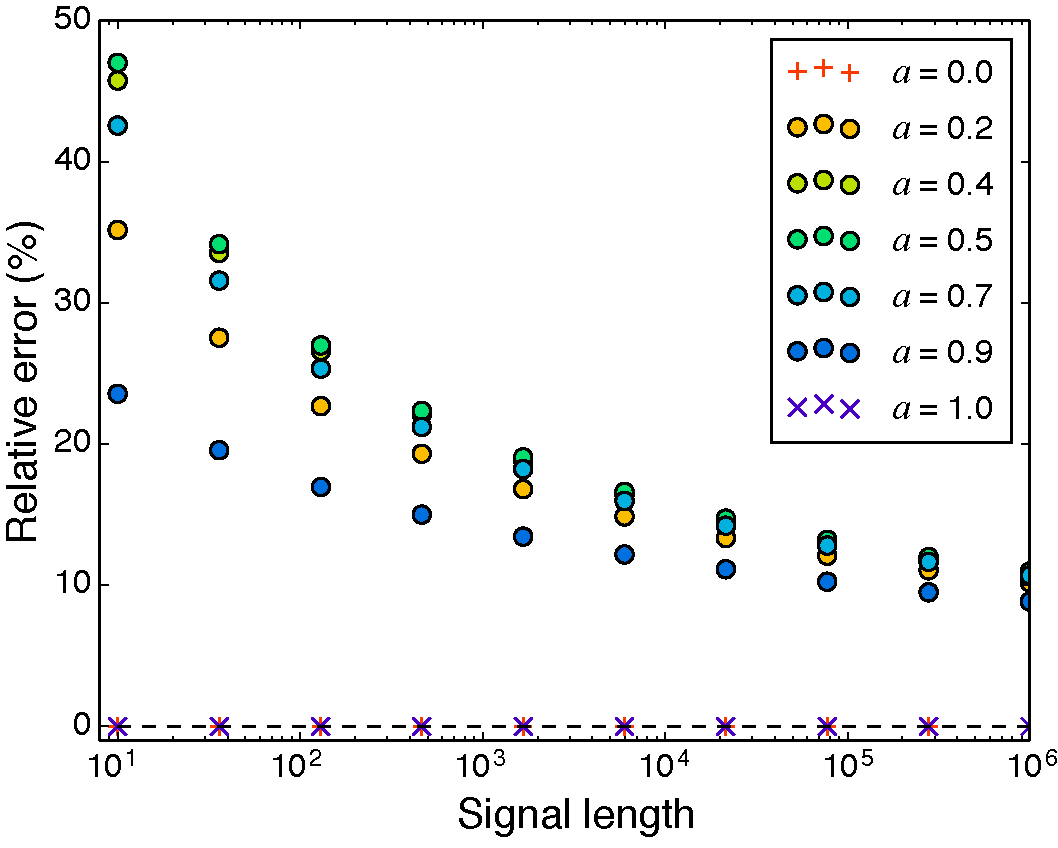
\includegraphics[width=0.5\linewidth]{Figures/convergence_even_N_abs_V2.pdf}
    \floatsource
    \label{fig:convergence_even_N_abs}
    \vspace{-0.3cm}
\end{figure}

\subsection{Polynomial representation}\label{subsec:poly}
The fractional shift matrix $ \mathbf{A}^a$ necessarily commutes with $ \mathbf{A} $, because $ \mathbf{A}^a\mathbf{A} = \mathbf{A}^{1 + a} = \mathbf{A}\mathbf{A}^a  $, so that $ \mathbf{A}^a $ is an LSI filter for signals on graphs having  $ \mathbf{A} $ as adjacency matrix (see~(\ref{eq:lsi_def})). Therefore, according to Theorem~\ref{theo:01}, $\mathbf{A}^a$ admits a polynomial representation like the one given in~(\ref{eq:filtro}). In what follows, we evaluate such a possibility for directed ring graphs and for arbitrary graphs.

\vspace{0.25cm}
\noindent\textbf{Directed ring graphs.} The adjacency matrix $ \mathbf{C} $ in~(\ref{eq:C}) of the directed ring graph with unitary weights satisfies $ char_\mathbf{C} = m_\mathbf{C} $ (due to the fact that the eigenvalues of  $\mathbf{C}$ are distinct). Therefore $ \mathbf{H} = \mathbf{C}^a $ can be directly expressed as a polynomial of degree up to  $(N-1)$ in $ \mathbf{C} $. In order to do this, we consider ~(\ref{eq:diag_C}) and the fact that $ \mathbf{F}^{-1} = \mathbf{F}^H $, with $ H $ indicating the conjugate transpose. This allows to show that  $ \mathbf{C}^a = \mathbf{F}^{H} \mathbf{\Lambda}^a_{\mathbf{C}} \mathbf{F}$ is a circulant matrix with the first column given by $ \mathbf{h}_a $ in (\ref{eq:DFT_inversa_autovalores}). Moreover, since the left product of a matrix by $\mathbf{C}$ produces a circular down-shift in each column of the matrix, the $ N $ powers of $\mathbf{C}$ form a basis for the space of $N\times N $ circulant matrices (note that $\mathbf{C}^N =  \mathbf{C}^0$ is the identity matrix). From the above, we conclude that the coefficients of the polynomial representation of $ \mathbf{C}^a $ are the entries of $ \mathbf{h}_a $, i.~e.
\begin{equation}\label{eq:poly_C}
    \mathbf{H} = \mathbf{C}^a = \sum_{\ell=0}^{N-1} h_a[\ell] \mathbf{C}^\ell.
\end{equation}

\noindent\textbf{Arbitrary graphs.} In order to demonstrate how to obtain the polynomial representation of $\mathbf{H}=\mathbf{A}^a$ for arbitrary graphs, let us consider another strategy to compute matrix functions. By definition, the minimal polynomial $m_{\mathbf{A}}(t)$ of $\mathbf{A}$ is the unique monic polynomial of lowest degree such that $m_{\mathbf{A}}(\mathbf{A})=\mathbf{0}$. By considering the Jordan canonical form of $\mathbf{A}$, it can be seen that
\begin{equation}
    m_{\mathbf{A}}(t)=\prod_{i=1}^s (t-\lambda_i)^{n_i}.
\end{equation}
It follows immediately that $m_{\mathbf{A}}$ is zero on the spectrum of $\mathbf{A}$, that is, the values computed in~(\ref{eq:defspec}) are all zero for $f(t)=m_{\mathbf{A}}(t)$. Given any polynomial $p$ and any matrix $\mathbf{A}\in\mathbb{C}^{N\times N}$, $p$ is clearly defined on the spectrum of $\mathbf{A}$ and $p(\mathbf{A})$ can be defined by substitution. For polynomials $p$ and $q$, $p(\mathbf{A})=q(\mathbf{A})$ if and only if $p$ and $q$ take the same values on the spectrum. Thus the matrix $p(\mathbf{A})$ is completely determined by the values of $p$ on the spectrum of $\mathbf{A}$. The following definition can then be established.
\vspace{0.2cm}
\begin{definition}\label{def:jc02}
    Let $f$ be defined on the spectrum of $\mathbf{A}\in\mathbb{C}^{N\times N}$. Then $f(\mathbf{A})\overset{\Delta}{=}p(\mathbf{A})$, where $p$ is the unique polynomial of degree less than $\sum_{i=1}^s n_i$ (which is the degree of the minimal polynomial) that satisfies the interpolation conditions
    \begin{equation}
        p^{(j)}(\lambda_i)=f^{(j)}(\lambda_i),\quad j=0:n_i-1,\quad i=1:s.
    \end{equation}
\end{definition}

The polynomial $p$ above is known as the Hermite interpolating polynomial. In particular, if $n_i=1$, $i=1,\ldots,s$, $p$ corresponds to the Lagrange interpolating polynomial
\begin{equation}
    p(t)=\sum_{i=1}^s f(\lambda_i)l_i(t),\quad l_i(t)=\prod_{j=1,j\neq i}^s \left(\frac{t-\lambda_j}{\lambda_i-\lambda_j}\right).
\end{equation}
In any case, the results briefly presented above lead us to conclude that $\mathbf{A}^a$ can be expressed as a polynomial in $\mathbf{A}$ and, therefore, according to Theorem~\ref{theo:01}, the fractional shift of a graph signal can be implemented as an LSI graph filter.

\section{Numerical Results}\label{sec:num}
The last section discussed the effect of applying a fractional shift to a graph signal and demonstrated that $\mathbf{A}^a$ admits a polynomial representation. In the first part of this section, a brief numerical example is presented to illustrate how the referred representation can be obtained. Then, the proposed fractional operator is applied in a context which brings to the front its practical advantage, namely the design of graph filters. Naturally, the resulting filter, being a polynomial in $\mathbf{A}^a$, could also be expressed as a polynomial in $\mathbf{A}$ and, therefore, it is a LSI filter.

\subsection{Example: Polynomial Representation of $\mathbf{A}^{a}$}\label{subsec:num1}
The graph considered in this example is shown in Fig.~\ref{fig:polyrepres} and has adjacency matrix
\begin{equation}\label{eq:ex001}
    %\setlength{\arraycolsep}{3pt}
    \mathbf{A}=\left[\begin{array}{ccccc}
            5  & 4  & 2  & 1  \\
            0  & 1  & -1 & -1 \\
            -1 & -1 & 3  & 0  \\
            1  & 1  & -1 & 2
        \end{array}\right].
\end{equation}
The entries of $\mathbf{A}$ in~(\ref{eq:ex001}) were chosen so that the Jordan decomposition of such a matrix had integer entries only. The referred decomposition is written using matrices
\begin{equation}\nonumber
    %\setlength{\arraycolsep}{3pt}
    \mathbf{V}=\left[\begin{array}{ccccc}
            -1 & 1  & 1  & 1 \\
            1  & -1 & 0  & 0 \\
            0  & 9  & -1 & 0 \\
            0  & 1  & 1  & 0
        \end{array}\right],\:\:
    %\setlength{\arraycolsep}{3pt}
    \mathbf{V}^{-1}=\left[\begin{array}{ccccc}
            0 & 1 & 1  & 1 \\
            0 & 0 & 1  & 1 \\
            0 & 0 & -1 & 0 \\
            1 & 1 & 1  & 0
        \end{array}\right]
\end{equation}
and
\begin{equation}
    %\setlength{\arraycolsep}{3pt}
    \mathbf{J}=\left[\begin{array}{ccccc}
            1 & 0 & 0 & 0 \\
            0 & 2 & 0 & 0 \\
            0 & 0 & 4 & 1 \\
            0 & 0 & 0 & 4
        \end{array}\right].
\end{equation}
Considering $f(t)=t^{0.3}$ and Definition~\ref{def:jc01}, $f(\mathbf{A})=\mathbf{A}^{0.3}$ can be computed according to
\begin{equation}\nonumber
    %\setlength{\arraycolsep}{2.5pt}
    \mathbf{A}^{0.3}=\mathbf{V}
    \left[\begin{array}{ccccc}
            f(1) & 0    & 0    & 0     \\
            0    & f(2) & 0    & 0     \\
            0    & 0    & f(4) & f'(4) \\
            0    & 0    & 0    & f(4)
        \end{array}\right]\mathbf{V}^{-1},
\end{equation}
which gives
\begin{equation}\nonumber
    %\setlength{\arraycolsep}{2.5pt}
    \mathbf{A}^{0.3}=
    \left[\begin{array}{ccccc}
            1.6294  & 0.6294  & 0.3448  & 0.2311  \\
            0       & 1.0000  & -0.2311 & -0.2311 \\
            -0.1137 & -0.1137 & 1.4020  & 0       \\
            0.1137  & 0.1137  & -0.1709 & 1.2311
        \end{array}\right].
\end{equation}
The same result can be achieved by using Definition~\ref{def:jc02}, which gives
\begin{align}
    p(\mathbf{A}) & =f(\mathbf{A})=\mathbf{A}^{0.3}\nonumber                                           \\
                  & =0.6688\mathbf{I}+0.3915\mathbf{A}-0.0654\mathbf{A}^2+0.0051\mathbf{A}^3,\nonumber
\end{align}
the polynomial representation of $\mathbf{A}^{0.3}$.

\begin{figure}
    \centering
    \caption{Directed graph used to illustrate how the corresponding fractional shift operator can be computed and represented in polynomial form.}
    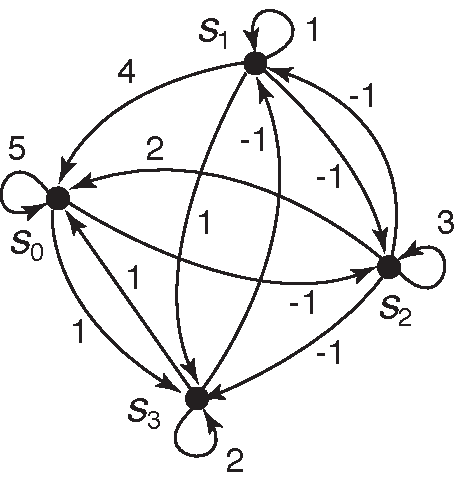
\includegraphics[width=0.35\linewidth]{Figures/graph_jordan.pdf}
    \floatsource
    \label{fig:polyrepres}
\end{figure}

\subsection{Least-square approximation of LSI filters}\label{subsec:lsi}
Before developing a numerical example illustrating the use of $\mathbf{A}^a$ to filter graph signals, let us first review a simple design technique that are least-squares approximations of ideal LSI filters~\cite{sandryhaila2014frequency}. Such a method consists of defining the (ideal) filter by specifying the values of $h(\lambda_i)$ (filter response in each eigenvalue of the shift operator), instead of determining the values of $h_{\ell}$ (filter coefficients). Describing the frequency response of the filter for each eigenvalue  $ \lambda_i $ yields the linear system of equations
\begin{equation}
    \label{eq:siseq}
    \begin{aligned}
        h(\lambda_0)     & = \alpha_0,     \\
        h(\lambda_1)     & = \alpha_1,     \\
                         & \vdots          \\
        h(\lambda_{N-1}) & = \alpha_{N-1}, \\
    \end{aligned}
\end{equation}
or, since $ h(\cdot) $ is a polynomial of degree $ L $,
\begin{equation}\label{eq:syst01}
    \begin{aligned}
        h_0 + h_1 \lambda_0 + \dots + h_L \lambda^L_0         & = \alpha_0,     \\
        h_0 + h_1 \lambda_1 + \dots  + h_L \lambda^L_1        & = \alpha_1,     \\
                                                              & \vdots          \\
        h_0 + h_1 \lambda_{N-1} + \dots + h_L \lambda^L_{N-1} & = \alpha_{N-1}. \\
    \end{aligned}
\end{equation}
Using a Vandermonde matrix constructed from the eigenvalues $\lambda_i$, the system~(\ref{eq:syst01}) can be written in matrix form as
\begin{equation}\label{eq:siseq2}
    \setlength{\arraycolsep}{3pt}
    \left[\begin{array}{ccccc}
            1 & \lambda_0     & \lambda^2_0     & \dots  & \lambda^L_0     \\
            1 & \lambda_1     & \lambda^2_1     & \dots  & \lambda^L_1     \\
              & \vdots        &                 & \vdots &                 \\
            1 & \lambda_{N-1} & \lambda^2_{N-1} & \dots  & \lambda^L_{N-1} \\
        \end{array}\right]
    \begin{bmatrix}
        h_0    \\
        h_1    \\
        \vdots \\
        h_L
    \end{bmatrix} =
    \begin{bmatrix}
        \alpha_0 \\
        \alpha_1 \\
        \vdots   \\
        \alpha_{N-1}
    \end{bmatrix}.
\end{equation}
More specifically, if one desires to design a low-pass filter (LPF) whose cutoff frequency is $ \lambda_{i_\text{cut}} $, one could set
\begin{equation}
    \label{eq:alfas}
    \alpha_j =
    \left\{\begin{array}{ll}
        1, & \text{for } j = 0,\ldots, i_\text{cut},    \\
        0, & \text{for } j = i_\text{cut}+1,\ldots,N-1.
    \end{array}\right.
\end{equation}
Since one generally has $ N \geq L+1$, the system of equations~(\ref{eq:siseq2}) is \emph{overdetermined} and does not have an exact solution. A possible strategy is to find coefficients $ h_\ell $, $ \ell=0, \dots, L$, that minimize, in the least-squares sense, the deviation from the ideal filter response. This corresponds to solve the optimization problem
\begin{equation}
    \label{eq:opt}
    \underset{\{h_\ell\}_{0, \dots, L}}{\text{min}} \sum_{n=0}^{N-1} \left( h(\lambda_n) - \alpha_n \right)^2.
\end{equation}

\noindent\textbf{Proposed application of the fractional shift.} The proposed change to the method above, which includes the fractional shift in the filter design, consists of replacing $\mathbf{A}$ with $\mathbf{A}^a$ in~(\ref{eq:filtro}), representing the LSI filter as
\begin{equation}
    \label{eq:filtrofracnew}
    h(\mathbf{A}^a) = \sum_{\ell=0}^{L} h_\ell \mathbf{A}^{a \cdot \ell}.
\end{equation}
If this is performed, the only adjustment needed in the technique described above consists of replacing the eigenvalues $\lambda_i$ with their $a^{\text{th}}$ powers $\lambda_i^a$ in~(\ref{eq:syst01}). The effect of such a substitution is illustrated and evaluated in what follows.

\subsection{Example: LS Approximation using $\mathbf{A}^{{a}}$}\label{subsec:lsi01}
In this example, we consider a network formed by $230$ weather stations that measure daily temperature across the United States~\cite{data2011}. Such stations are represented by the vertices of an undirected graph whose edges have been established by using the $8$-nearest neighbor criterion.  The edge connecting vertices $v_n$ and $v_m$ is weighted according to
\begin{equation}
    \mathbf{A}_{n,m}=\frac{e^{-d^2_{n,m}}}{\sqrt{\sum_{k\in\mathcal{N}_n}e^{-d^2_{n,k}}\sum_{\ell\in\mathcal{N}_m}e^{-d^2_{n,\ell}}}},
\end{equation}
where $d_{n,m}$ denotes the geodesical distance between the $n^{\text{th}}$ and the $m^{\text{th}}$ sensors. The snapshot of all measurements taken on February $1^{\text{st}}$, 2003 forms the signal indexed by the referred graph, which is shown in Fig.~\ref{fig:usa00}. From the GFT of the signal, which is plotted in Fig.~\ref{fig:usa01}, it can be seen that its spectral content is concentrated in the low graph frequencies. Note that such frequencies correspond to the eigenvalues of $\mathbf{A}$, which are marked along the horizontal axis of the figure; additionally, the referred marking accompanies the fact that low (resp. high) graph frequencies are associated with higher (resp. lower) eigenvalues~\cite{sandryhaila2014frequency}.

\begin{figure}%
    \centering
    \caption{Graph of a network formed by $230$ weather stations measuring the temperature across the United States. The snapshot of all measurements taken on February $1^{\text{st}}$, 2003 is the corresponding graph signal.}%
    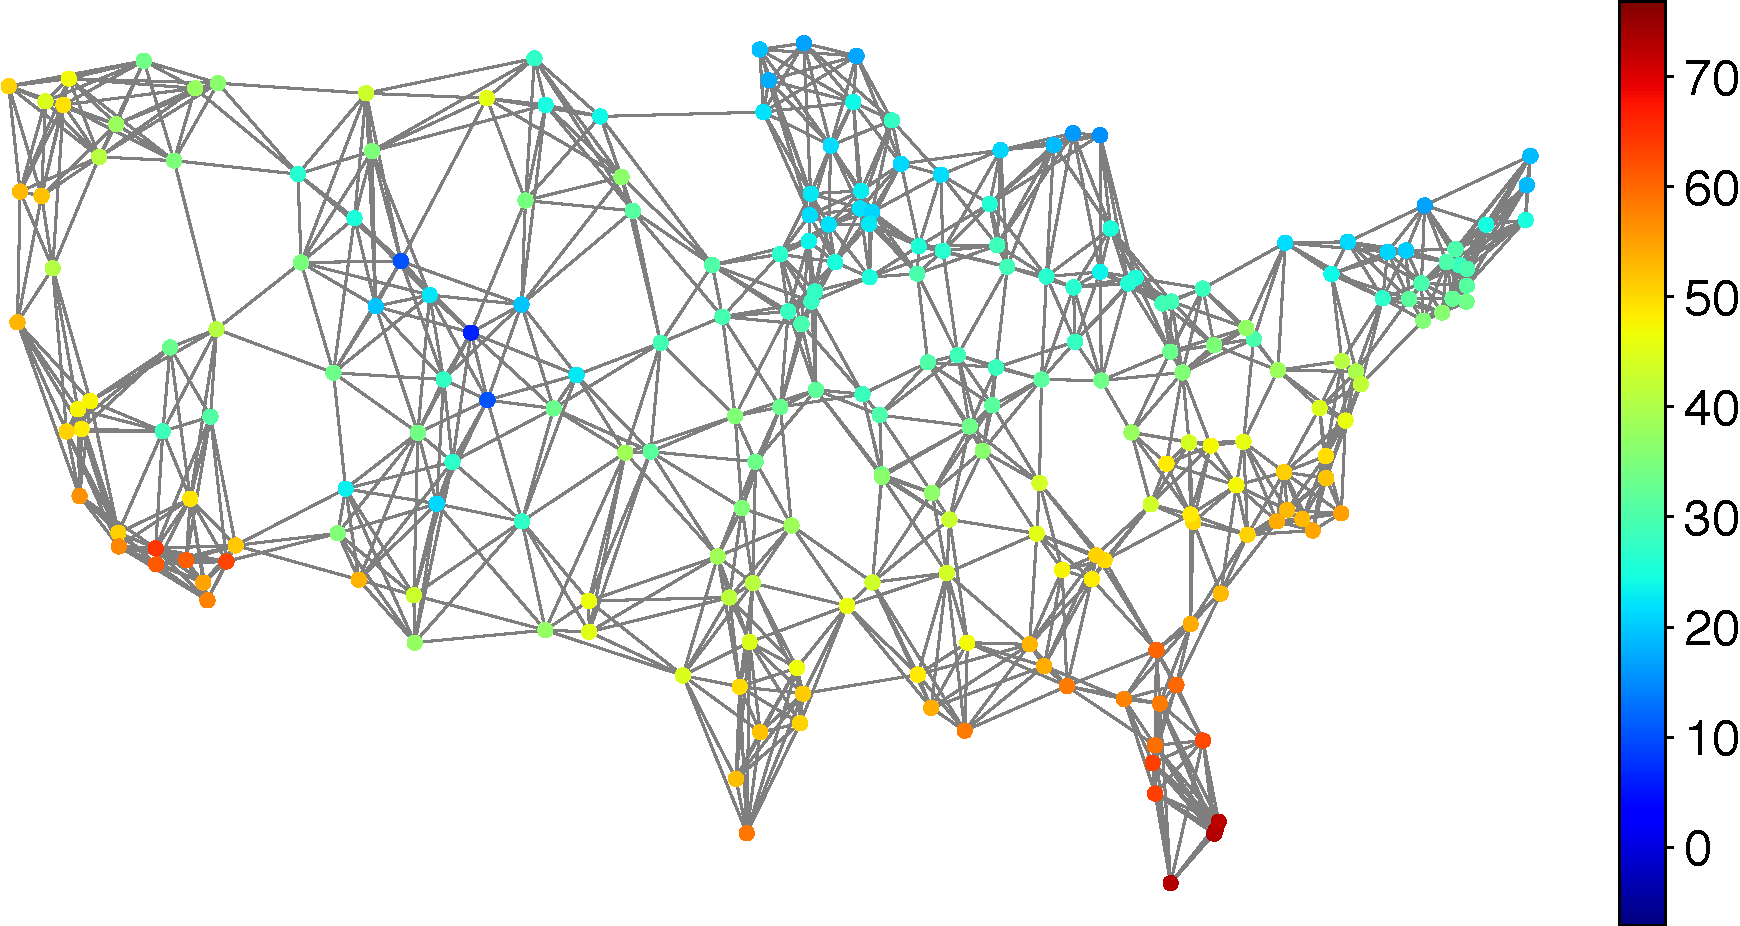
\includegraphics[width=0.6\linewidth]{Figures/GNorm_estacoes_temperatura.pdf}
    \floatsource
    \label{fig:usa00}%
    \vspace{0.14cm}
\end{figure}

\begin{figure}[ht!]%
    \centering
    \caption{Magnitude of the graph Fourier transform of the signal in Fig~\ref{fig:usa00}. The graph frequencies correspond to the eigenvalues of $\mathbf{A}$; low (resp. high) graph frequencies are associated with higher (resp. lower) eigenvalues.}%
    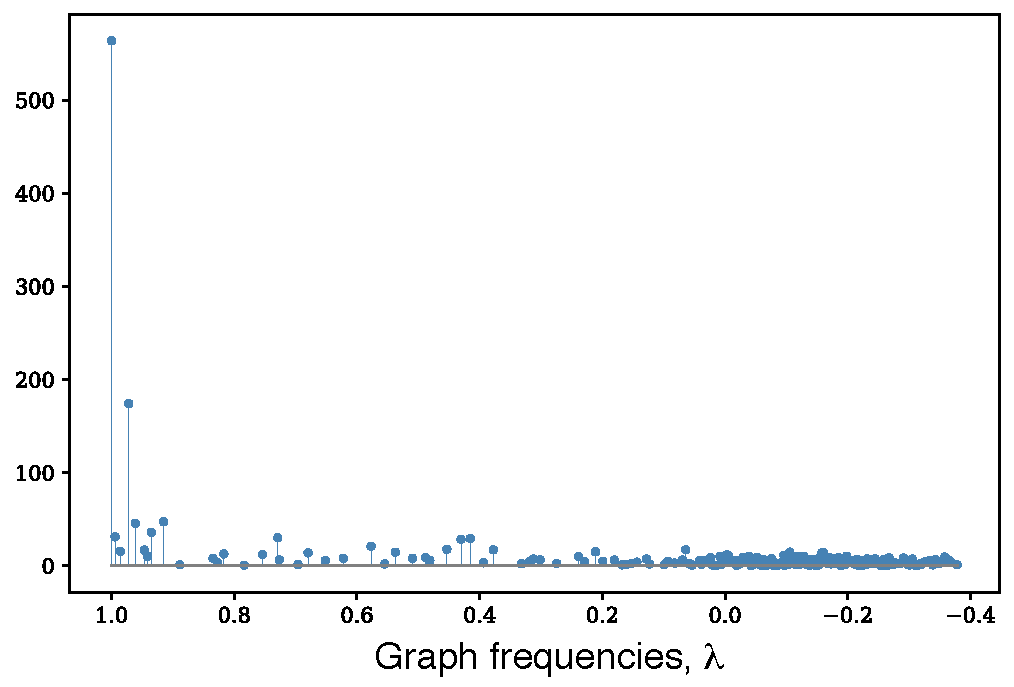
\includegraphics[width=0.5\linewidth]{Figures/GNorm_estacoes_GFT_Temperatura.pdf}%\vspace{-0.1cm}
    \floatsource
    \label{fig:usa01}%
    %\vspace{-0.2cm}
\end{figure}

\begin{figure}[ht!]
    \centering
    \caption{Fractional parameters providing the minimum approximation errors, for different values of $L$, between the ideal LPF and the filter designed by using the fractional graph shift operator $\mathbf{A}^a$.}%
    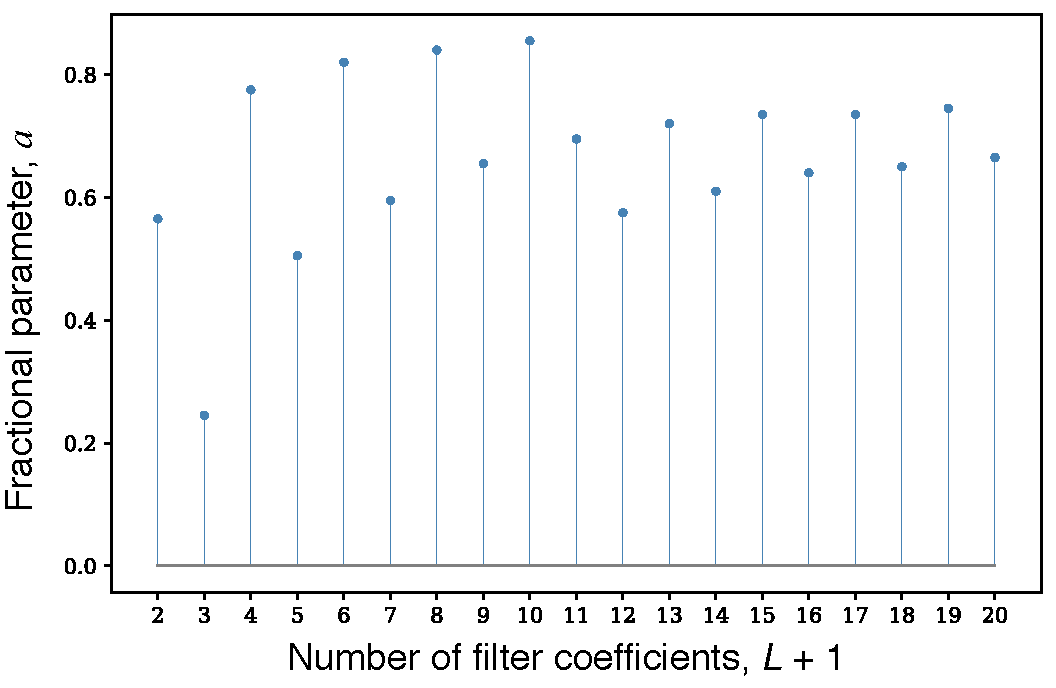
\includegraphics[width=0.5\linewidth]{Figures/ERROR_ordens_fracionarias.pdf}
    \floatsource
    \label{fig:usa02}%
    %\vspace{-0.5cm}
\end{figure}

We then use the strategy explained in Subsection~\ref{subsec:lsi} to design a filter that approximates an ideal low-pass filter with $\lambda_{i_\text{cut}}=0.2$. In this case, $i_\text{cut}=39$ so that the $40$ lowest graph frequencies are (ideally) preserved after the signal is filtered. We considered approximations with $L$ ranging from $1$ to $19$, that is, filters with $2$ to $20$ coefficients. For each of these values, we varied the fractional parameter $a$ from $0$ to $1$ and, in~(\ref{eq:siseq2}), after replacing $\lambda_i$ with $\lambda_i^a$, $i=0,1,\ldots,N-1$, and solving~(\ref{eq:opt}),\footnote{The optimization problem~\ref{eq:opt} has been solved using the Linear Algebra module \emph{linalg} for Scipy, a free and open-source Python library used for scientific and technical computing. In all experiments performed, the least mean squares algorithm converged and the time required for this was negligible, considering the addressed application scenario.} we registered the value of $a$ providing the minimum error between the designed filter and the ideal filter. At the end of this procedure, the plot shown in Fig.~\ref{fig:usa02} was produced. Observing the figure, we verify that, for any value of $L$, the best approximation is provided when $a\neq1$. This is enough to conclude that, for the graph considered in the example, the use of a fractional version $\mathbf{A}^a$, $a\neq 1$, of $\mathbf{A}$ always provides a better result than the one obtained with the non-fractional matrix. A visual comparison between these alternatives can be performed from Fig.~\ref{fig:usa03}, where we show the (minimum) errors we have just referred to together with the errors when the original (non-fractional) matrix $\mathbf{A}$ is employed.

In Fig.~\ref{fig:usa04}, we can observe the ideal filter response superimposed on the responses obtained when $\mathbf{A}$ and $\mathbf{A}^a$ are used to design a filter with $L+1=10$ coefficients. In this case, the fractional parameter providing the minimum error is $a=0.855$. In the figure, we notice that the filter designed with $\mathbf{A}^a$ has fluctuations that deviate less from the ideal filter, when compared to those related to the filter designed using $\mathbf{A}$. This can be observed mainly in the passband and constitutes a visual result coherent with the obtained approximation errors. Plots with similar behavior are obtained for other values $L$.

\begin{figure}[t!]
    \centering
    \caption{Minimum approximation (mean squared) errors, for different values of $L$, between the ideal LPF and the filters designed by using the fractional graph shift operator $\mathbf{A}^a$ and the non-fractional operator $\mathbf{A}$.}%
    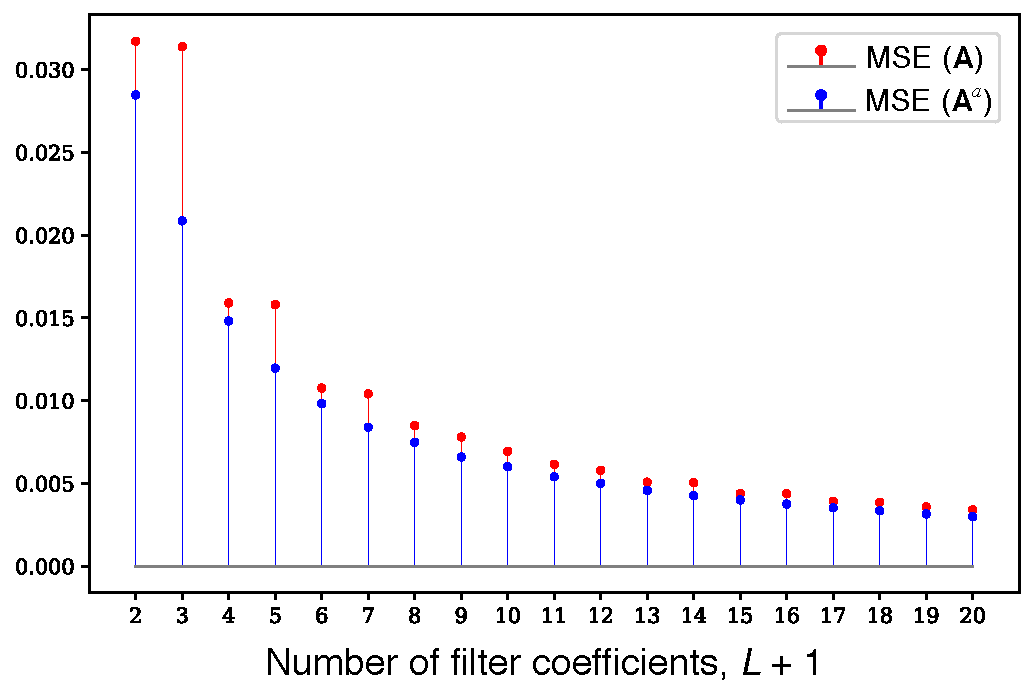
\includegraphics[width=0.65\linewidth]{Figures/ERROR_mse_min.pdf}
    \floatsource
    \label{fig:usa03}%
    %\vspace{-0.2cm}
\end{figure}

\begin{figure}[t!]
    \centering
    \caption{Ideal filter response superimposed on the responses obtained when $\mathbf{A}$ and $\mathbf{A}^a$, $a=0.855$, are used to design a filter with $L+1=10$ coefficients.}
    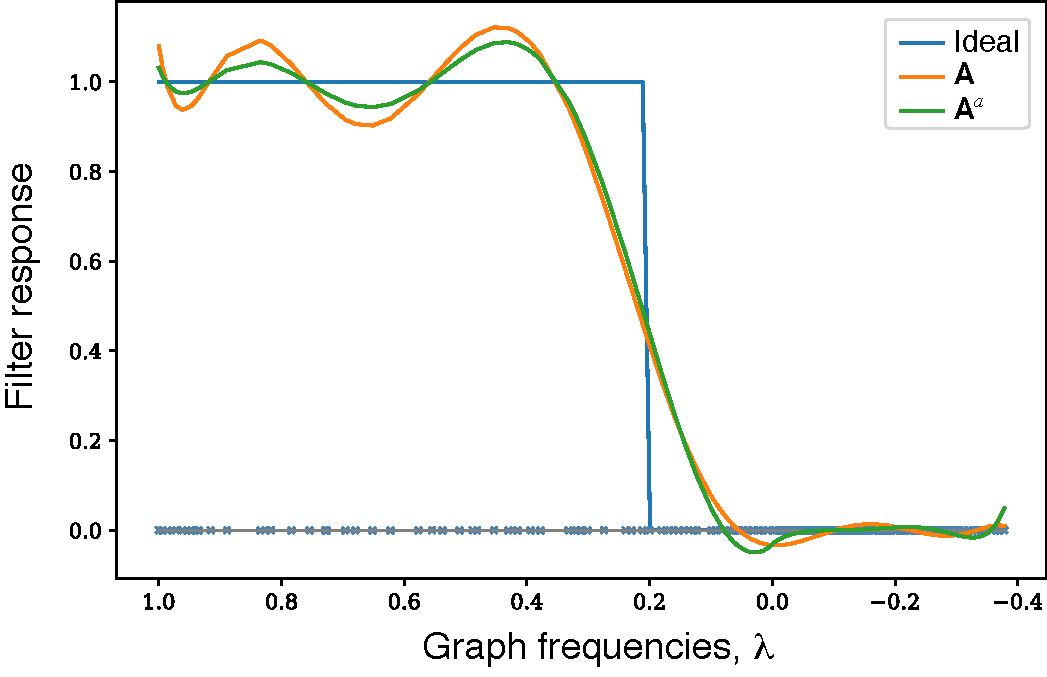
\includegraphics[width=0.65\linewidth]{Figures/ERROR_estacoes_resposta_grau10.pdf}%\vspace{-0.4cm}
    \floatsource
    \label{fig:usa04}%
    %\vspace{-0.2cm}
\end{figure}

\subsection{Example: noise removal via LSI low-pass filtering}\label{subsec:lsi02}
In this example, we start from the same graph signal considered in Subsection~\ref{subsec:lsi01}. We add to the samples of the referred signal random uniformly-distributed values whose amplitude corresponds to a percentage of the range of the signal itself. Such a synthetic noise addition is intended to simulate what happens in many practical scenarios, in which measurements performed on a sensor network are subject to different sources of distortion. The resulting noisy signal is then filtered by the filters shown in Fig.~\ref{fig:usa04}, as an attempt to reduce the influence of the noise and recover the original signal.

During the experiment, the aforementioned percentage was varied from $1\%$ to $50\%$ and, for each of these values, $100$ noisy signals were generated. After low-pass filtering, the mean squared error between the original and filtered graph signals were computed. The results show that the filter designed using $\mathbf{A}^{0.855}$ allows to recover the signal with average reconstruction error always smaller than that with the filter designed using $\mathbf{A}$; see the data in Fig.~\ref{fig:usa05}.

{In this context, it is relevant to remark that the (best) fractional parameter $a=0.855$ has been found using the strategy described in the second paragraph of Subsection~\ref{subsec:lsi01}, which depends on the error between the designed filter and the ideal filter only. Therefore, the referred choice does not require prior knowledge of the original signal beforehand, which is usually not available in real-world problems.} This illustrates the potential gain that can be achieved, in this application scenario, when considering the possibility of fractionalization of the graph shift operator.

    {Finally, it is also interesting to mention that only one or a few nodes could have had their measurements corrupted by noise or changed due to other factors; this would represent, for instance, a scenario in which certain sensors would be malfunctioning. In order to obtain some preliminary results taking into account the above described assumption, additional simulations were carried out. The previous tests were repeated, but assuming that only a number from $1$ to $12$ nodes had their values nullified or increased by $20$ times. We then performed a low-pass filtering, expecting that the high-frequency component associated with the referred measurement changes would be attenuated and that the smooth behavior of the signal would be recovered. In general, the results obtained using the proposed fractional operator were better or at least equivalent to those obtained with the corresponding ordinary operator. Future works may address this issue in more detail.}

\begin{figure}[t!]
    \centering
    \caption{Reconstruction (mean squared) errors after a noise removal procedure is performed by using graph filters with $L+1=10$ coefficients and designed from $\mathbf{A}$ and $\mathbf{A}^a$, $a=0.855$.}%
    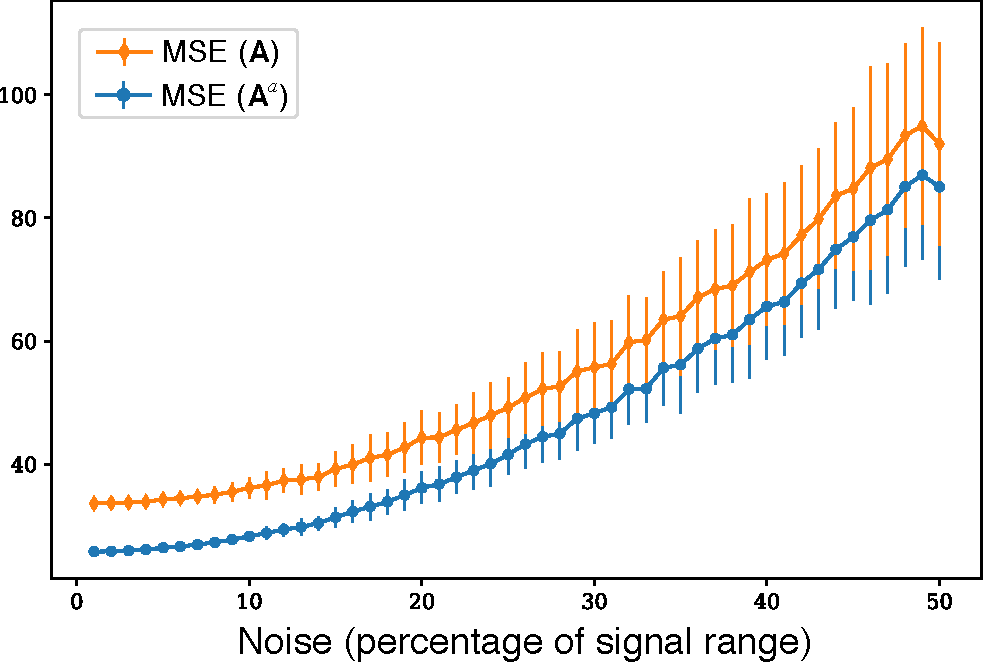
\includegraphics[width=0.7\linewidth]{Figures/ERROR_errobar_filtrados.pdf}
    \floatsource
    \label{fig:usa05}%
    \vspace{-0.1cm}
\end{figure}

\section{Concluding remarks}\label{sec:conc}
This chapter proposed and discussed the fractional shift operator of graph signals. The core idea for the contribution was that, in the GSP theory, the unit shift is defined from the adjacency matrix of a graph. Interpreting the fractional shift as a filtering operation, it was demonstrated that, for ring graphs, its application produces the expected effect of approximating the classical ideal interpolating filter, exhibiting satisfactory results for bandlimited signals. Moreover, it was also shown that the referred fractional operator can be implemented as an LSI graph filter for arbitrary graphs and real-world examples were presented, illustrating the benefits of using $\mathbf{A}^a$ to design graph filters for noise removal.

\chapter{The fractional quaternion discrete Fourier transform and its applications}
\label{ch:FrQDFT}

Linear discrete transforms are building blocks for a multitude of techniques in the field of signal processing, being almost as important as they are diverse. Among the factors which distinguish one from the others, there is the algebraic structure over which they are defined, e.~g. a finite field and its extensions (such as in number-theoretic \cite{blahut2010fast,pedrouzo2017number,chandra2014exact,lima2013} and arithmetic \cite{knockaert1994generalized, rajapaksha2014vlsi} transforms), or the real and complex fields (as in the usual discrete Fourier transform). Let us recall an important point that has already been made: as the algebra is extended (for instance, from $ \mathbb{R} $ to $ \mathbb{C} $), it is possible to encode more information into each signal sample. Such was the motivation behind Sangwine's definition \cite{sangwine1996fourier} of discrete two-dimensional quaternion transforms, based on their continuous counterparts previously defined by Ell \cite{ell1993quaternion}: to apply these four-dimensional numbers --- the quaternions, an extension of the complex field --- to color image processing. Since then, quaternion transforms have been useful not only to image processing \cite{ell2007hypercomplex,chen2018quaternion,li2013quaternion,evans2000hypercomplex,silva2018}, but also to other fields, such as bivariate signal analysis \cite{flamant2017spectral,flamant2017time,flamant2018complete}.

Fractional transforms are yet another class of tools of great use, the reader may remember the review presented in Chapter \ref{ch:reviewGSP}. Regarding quaternion transforms, a couple of competent works have already addressed their fractionalization \cite{guanlei2008fractional, wei2013different, roopkumar2016quaternionic} and some applications have been proposed \cite{chen2018quaternion}. However, the author is not aware of papers approaching fractional quaternion discrete transforms \textit{from an eigenstructure analysis point of view}. This reasoning may unfold new theoretical insights and implementation techniques, and such is the motivation for this work.

In this chapter, the eigenstructure of the quaternion discrete Fourier transform (QDFT) matrix is investigated and shown to be closely related to that of the unitary discrete Fourier transform (DFT). This result offers an approach for defining the fractional version of the QDFT (referred to as FrQDFT). Following the central goal of defining the transform through eigendecomposition theory, a generalization is proposed in the form of a multiparametric fractional quaternion discrete Fourier transform (MFrQDFT). For illustrative purposes, this work proposes and briefly explores an encryption scheme for color images with opacity layer, fully harnessing the holistic processing of 4-channels 2D signals through the MFrQDFT.

The proposed method for image encryption fits in the class of schemes that use linear transforms alongside non-linear blocks \cite{hsue2018enhancing}, to implement confusion and diffusion. The currently available methods in the state-of-the-art literature respond to a diverse range of needs, as fast implementation through parallel computing \cite{wang2019fast}, increased safety and robustness by using matrix semi-tensor product \cite{wang2020image} or one-time keys \cite{liu2010}, just to name a few examples. The main scope of this chapter is not the encryption scheme \textit{per se}, but rather the FrQDFT eigenscructure and the MFrQDFT definition, the latter having the image encryption as a framework to showcase some of its possibilities. Nevertheless, the proposed encryption algorithm is described and evaluated to some extent. Although being an illustrative scenario, it stands on tools adopted currently by the literature. For example, the chosen method for key generation involved the use of chaotic maps, known to help achieving high bit sensibility and large key space. It follows works such as the one by Liu and Wang \cite{liu2011color}, which proposed a color image encryption scheme using two chaotic maps and one-time keying, aiming to achieve large key space and cycle lengths. Another work by Liu and Wang \cite{liu2012} employed a piecewise linear chaotic map and DNA encoding for ensuring the initial conditions of the encryption change according to the image, whereas Wang \textit{et al.} \cite{wang2010chaotic} used a Lorentz chaotic map and a perceptron model applied to image encryption. The proposed scheme uses a chaotic tent map to generate a pseudo-random sequence, from which the secret parameters are extracted.


This chapter is structured as follows. Section \ref{sec:autoestrutura} presents the usual definition of the QDFT and proves the central theorem of this work, regarding how the DFT and QDFT share symmetric eigenvectors; it closes with comments on the quaternion representation of color images with opacity layer. Section \ref{sec:FrQDFT} discusses the fractionalization of the QDFT from an eigenstructure point of view and demonstrates some properties purely based on matrix algebra. Section \ref{sec:multi} proposes a multiparametric extension of the fractional transform and presents an application involving encryption of color images with opacity layer. The main results are summarized in Section \ref{sec:conclusao}.


\section{Eigenstructure of the QDFT}
\label{sec:autoestrutura}
Let us recall the definition of the 1D left QDFT of axis $ \qmu $ -- a unit pure quaternion, as presented in \cite[Sec. 3.3.1]{ell2014quaternion} and in (\ref{eq:QDFT_fwd}). The $ m$-th entry of the QDFT of vector $ \mathbf{v} $ is
\begin{equation}
\label{eq:QDFT_fwd}
\!\widehat{v}_m \!=\! \text{QDFT}\{ \mathbf{v} \}_m \!\overset{\Delta}{=}\! \frac{1}{\sqrt{N}} \!\sum_{n=0}^{N-1}  \exp \left( -\qmu \frac{2\pi}{N} nm \right) v_n \!\in\! \mathbb{C}_{\qmu},\!
\end{equation}
in which $ \mathbb{C}_{\qmu} $ denotes the set of numbers $ a + \qmu b $, $ a,b \in \mathbb{R} $, isomorphic to the complex set. It matters to notice that, due to the lack of commutativity in quaternion multiplication, the position of the kernel relative to the operand in (\ref{eq:QDFT_fwd}) is relevant and must be kept consistent along all computations. Hence, the inverse transformation must be computed with the kernel on the same relative position,
\begin{equation}
\label{eq:QDFT_inv}
v_n = \text{QDFT}^{-1}\{ \widehat{\mathbf{v}} \}_n = \frac{1}{\sqrt{N}}\sum_{m=0}^{N-1}  \exp \left( \qmu \frac{2\pi}{N} nm \right) \widehat{v}_m.
\end{equation}

The synthesis and analysis equations may be written in matrix form as
\begin{equation}
\label{eq:QDFT}
\widehat{\mathbf{v}} = \text{QDFT}\{ \mathbf{v} \} = \mathbf{F} \mathbf{v},
\end{equation}
\begin{equation}
\label{eq:QDFT_mtx_inv}
\mathbf{v} = \text{QDFT}^{-1}\{ \widehat{\mathbf{v}} \} = \mathbf{F}^{-1} \widehat{\mathbf{v}},
\end{equation}
where $ \mathbf{F} $ is the unitary QDFT matrix, with entries $ \{\mathbf{F}\}_{n,m} = \sqrt{N}^{-1} \exp \left( -\qmu \frac{2\pi}{N} nm \right)$. Since $ \exp \left( -\qmu \frac{2\pi}{N} \right) $ is an $ N $-th root of unity, such as $ \exp \left( -\qi \frac{2\pi}{N} \right) $, it follows that $ \mathbf{F} $ shares many properties of the DFT matrix, such as invertibility (simple calculations show that $ \mathbf{F}^{-1} = \mathbf{F}^{H} $), what guarantees validity of the inversion formulae in (\ref{eq:QDFT_inv}) and (\ref{eq:QDFT_mtx_inv}).

The two-dimensional QDFT can be defined in a similar fashion, although more options regarding kernel positioning are available, since for any pure quaternions $ \qmu \neq \qnu $, one may verify that generally $ e^{\qnu \alpha} e^{\qmu \beta} \neq e^{\qnu \alpha + \qmu \beta} $. Ell and Sangwine \cite{ell2014quaternion} presented the \textit{eight} distinct ways of building a 2D-QFT, which translate directly into options for 2D-QDFT. One of such possibilities is to transform the quaternion-valued matrix $ \mathbf{X} \in \mathbb{H}^{N\times M}$ according to the equation
\begin{equation}
\label{eq:2DQDFT-01}
\widehat{X}_{u,k} = 
\text{2D-QDFT}\{ \mathbf{X} \}_{u,k} \!\overset{\Delta}{=}\! \frac{1}{\sqrt{MN}} \!\sum_{n=0}^{N-1} \sum_{m=0}^{M-1}  \exp \left( -\qmu \frac{2\pi}{N} nu \right) X_{n,m} \exp \left( -\qnu \frac{2\pi}{M} mk \right).
\end{equation}
This formulation of the 2D-QDFT translates into the following matrix equation,
\begin{equation}
\label{eq:2DQDFT-02}
\widehat{\mathbf{X}} = \mathbf{F}^{(\qmu)} \mathbf{X} \mathbf{F}^{(\qnu)},
\end{equation}
where the Fourier matrices are similar to the one used in (\ref{eq:QDFT}), except from the pure quaternion which serves as transform axis (shown in the parenthesis). This is a consequence of the \textit{separability} of the 2D-QDFT, by which this transform may be conceived as the successive application of two 1D-QDFTs: once in the rows of $ \mathbf{X} $, once in the columns. Therefore, some results and properties derived for the 1D-QDFT may naturally extend to the two-dimensional case.

The similarities between the QDFT and the DFT matrices hugely aid the investigation of the eigenstructure of matrix $ \mathbf{F} $. As a result of Theorem \ref{th:01}, which is a contribution of this thesis, one is able to deduce the QDFT eigenstructure out of even and odd DFT eigenvectors, by using a variation of Pei's reasoning regarding the 2D-QDFT \cite{pei2010eigenfunctions}.

\begin{theorem}
\label{th:01}
Let $ \mathbf{v} $ be an eigenvector of the unitary DFT with eigenvalue $ \lambda $.
\begin{itemize}[noitemsep]
\item[(a)] If $ \mathbf{v} $ has even symmetry (in which case $ \lambda = \pm 1 $), then it is also an eigenvector of the QDFT with eigenvalue $ \lambda $.
\item[(b)] If $ \mathbf{v} $ has odd symmetry (in which case $ \lambda = \pm \qi $), then it is also an eigenvector of the QDFT (of axis, let us say, $ \qmu $) with eigenvalue $ -\lambda \qi \qmu$, i.~e., $ \pm \qmu $.
\end{itemize}
\end{theorem}

\begin{proof}
\begin{itemize}
\item[(a)] If $ \mathbf{v} $ has even symmetry, i.~e., $ v_n = v_{N-n} $ for $ n=1,\dots,N-1 $, then
\begin{equation}
%\label{key}
\sum_{n=0}^{N-1} v_n \sin \frac{2\pi}{N} nm = 0,
\end{equation}
therefore,
\newcommand{\correctinghspace}{-1.8cm}
% \begin{equation*}
%\small
% \label{eq:15}
\begin{align*}
\sqrt{N} \text{QDFT}\{ \mathbf{v} \}_m &= \sum_{n=0}^{N-1} v_n e^{-\qmu \frac{2\pi}{n} nm} \\
&\hspace{\correctinghspace}
=\sum_{n=0}^{N-1} v_n \left( \cos \frac{2\pi}{n} nm - \qmu \sin \frac{2\pi}{n} nm \right) \\
&\hspace{\correctinghspace}
= \left( \sum_{n=0}^{N-1} v_n \cos \frac{2\pi}{n} nm \right) - \underbrace{\left(  \sum_{n=0}^{N-1} v_n \sin \frac{2\pi}{n} nm \right)}_{=0} \qmu \\
&\hspace{\correctinghspace}
= \left( \sum_{n=0}^{N-1} v_n \cos \frac{2\pi}{n} nm \right) - \underbrace{\left(  \sum_{n=0}^{N-1} v_n \sin \frac{2\pi}{n} nm \right)}_{=0} \qi \\
&\hspace{\correctinghspace}
= \sqrt{N} \text{DFT}\{ \mathbf{v} \}_m = \sqrt{N} \lambda v_m \\
&\hspace{\correctinghspace}
\Rightarrow \text{QDFT}\{ \mathbf{v} \} = \lambda \mathbf{v}.
\end{align*}
% \end{equation*}
\item[(b)] If $ \mathbf{v} $ has odd symmetry, i.~e., $ v_n = -v_{N-n} $ for $ n=1,\dots,N-1 $ and $ v_0 = 0 $, then
\begin{equation}
%\label{key}
\sum_{n=0}^{N-1} v_n \cos \frac{2\pi}{N} nm = 0,
\end{equation}
hence,
\begin{equation}
\small
\label{eq:17}
\begin{aligned}
\sqrt{N} \text{QDFT}\{ \mathbf{v} \}_m &= \sum_{n=0}^{N-1} v_n e^{-\qmu \frac{2\pi}{n} nm}\\
&\hspace{\correctinghspace}
=
\sum_{n=0}^{N-1} v_n \left( \cos \frac{2\pi}{n} nm - \qmu \sin \frac{2\pi}{n} nm \right) \\
&\hspace{\correctinghspace}
= {\underbrace{\left( \sum_{n=0}^{N-1} v_n \cos \frac{2\pi}{n} nm \right)}_{=0} - \left(  \sum_{n=0}^{N-1} v_n \sin \frac{2\pi}{n} nm \right) \qmu }\\
&\hspace{\correctinghspace}
= - \left(  \sum_{n=0}^{N-1} v_n \sin \frac{2\pi}{n} nm \right) \qmu.
\end{aligned}
\end{equation}

But, from the odd symmetry assumption,
\begin{equation}
%\label{key}
\begin{aligned}
\sqrt{N}\lambda v_m = \sqrt{N}\text{DFT}\{ \mathbf{v} \}_m &= \sum_{n=0}^{N-1} v_n e^{-\qi \frac{2\pi}{n} nm}= - \left(  \sum_{n=0}^{N-1} v_n \sin \frac{2\pi}{n} nm \right) \qi,
\end{aligned}
\end{equation}
therefore (remember that $ \lambda $ and $ v_m $ commute)
\begin{equation}
\label{eq:19}
\sum_{n=0}^{N-1} v_n \sin \frac{2\pi}{n} nm = \sqrt{N}v_m \lambda \qi.
\end{equation}
From (\ref{eq:17}) and (\ref{eq:19}),
\begin{equation}
\label{eq:20}
\begin{aligned}
\sqrt{N}\text{QDFT}\{ \mathbf{v} \}_m &=  -\sqrt{N}\text{DFT} \{ \mathbf{v} \}_m \qi \qmu \\
&\hspace{\correctinghspace}
= -\sqrt{N}v_m \lambda \qi \qmu \\
&\hspace{\correctinghspace}
\Rightarrow \text{QDFT}\{ \mathbf{v} \} = -\lambda \qi \qmu \mathbf{v}.
\end{aligned}
\end{equation}
\end{itemize}
\end{proof}

The results of Theorem \ref{th:01} are summarized in Table \ref{tab:01}.
This analysis can immediately be extended to the two-dimensional case if one considers the separability of the 2D-QDFT, mentioned after (\ref{eq:2DQDFT-02}). If $ (\mathbf{e}^{(\qmu)}, \lambda_{\qmu}) $ and $ (\mathbf{e}^{(\qnu)}, \lambda_{\qnu}) $ are (column-)eigenvector-eigenvalue pairs of the matrices $ \mathbf{F}^{(\qmu)} $ and $ \mathbf{F}^{(\qnu)} $, respectively, then the 2D signal $ \mathbf{e}^{(\qmu)} \mathbf{e}^{(\qnu)^T}  $ is a 2D-QDFT eigenvector with eigenvalue $ \lambda_{\qmu} \lambda_{\qnu} $ \cite{candan2011}. Therefore, this 2D-QDFT has eight (possibly) distinct eigenvalues: $ \pm 1, \pm \qmu, \pm \qnu, \pm \qmu \qnu $.

\begin{table}[b!]
\center
\captionof{table}{DFT and QDFT eigenvectors.}
\label{tab:01}
\begin{tabular}{ccc}
\toprule
\shortstack{Eigenvector\\ symmetry} & \shortstack{Eigenvalue\\(DFT)} & \shortstack{Eigenvalue\\(QDFT)} \\
\midrule
Even & $ \pm 1 $ & $ \pm 1 $ \\
Odd & $ \pm \qi $ & $ - (\pm \qi) \qi \qmu = \pm \qmu $\\
\bottomrule
\end{tabular}
\end{table}

\subsection{2D-QDFT and color images with opacity layer}
\label{subsec:2D_QDFT}
The 2D-QDFT has been commonly used to process color images, which are represented as matrices of pure quaternions \cite{lu20072d,ell2006hypercomplex,chen2018multiple}. In this representation, each color channel of a certain pixel corresponds to an imaginary component of the pure quaternion. Although this mapping is useful and adequate, it neglects the quaternion scalar part (always set to zero), causing a difference in dimensionality between input and output of the 2D-QDFT: while the image is a 2D signal with three-dimensional components, its spectrum has four-dimensional entries. It surely is not a problem \textit{per se}, rather is an inconvenience, also found when processing real signals with the DFT.

An application free from this inconvenience is the analysis of color images with opacity (or alpha) layer, as in files in portable network graphics format (PNG). In this case, each pixel $ (R,G,B,\alpha) $ is mapped into $ q = \alpha + R \qi + G \qj + B \qk $, forming the quaternion-valued matrix $ \mathbf{X} $. Let us compute the 2D-QDFT by separately transforming the rows and columns using (\ref{eq:2DQDFT-02}), with the same transform axis on both sides,
\begin{equation}
\label{eq:2DQDFT}
\text{2D-QDFT}\{\mathbf{X} \} = \mathbf{F} \mathbf{X} \mathbf{F}^T.
\end{equation}

One should notice that the transformation in (\ref{eq:2DQDFT}) does \textit{not} consist on the successive application of the \textit{same} QDFT to the rows and columns of matrix $ \mathbf{X} $. Due to the noncommutative nature of quaternion multiplication, as it was previously mentioned, different transforms are obtained when choosing between left- or right-multiplications, even though the transform axis is kept unchanged. The operation in (\ref{eq:2DQDFT}) performs a \textit{left} QDFT on the columns and a \textit{right} QDFT on the rows, as it is clear from (\ref{eq:2DQDFT-01}). A 2D-QDFT consisting of the \textit{same} transformation applied in both dimensions must use multiplications with the same orientation, e.~g.
\begin{equation}
\label{eq:2DQDFTv2}
\mathbf{F} \left( \mathbf{F}\mathbf{X}^T \right)^T.
\end{equation}

Fig. \ref{fig:2D_QDFTv1} shows the QDFT -- according to (\ref{eq:2DQDFT}) -- of Fig. \ref{fig:dice}, as another PNG image. As an illustration of the difference in using (\ref{eq:2DQDFT}) or (\ref{eq:2DQDFTv2}), caused by the lack of commutativity in quaternion multiplication, the mean squared error (MSE) between the two spectra was computed. The result was approximately 1070.

\begin{figure}
\centering
\caption{(a) 2D-QDFT of the PNG image in Fig. \ref{fig:dice}, according to (\ref{eq:2DQDFT}), with axis $ \qmu = \frac{1}{\sqrt{3}}(\qi + \qj + \qk) $. (b) 2D-QDFT of the same image, same transform axis, following the approach in (\ref{eq:2DQDFTv2}).}
\subfloat[\label{fig:2D_QDFTv1}]{

\includegraphics[width=0.3\linewidth]{Figures/2D_QDFTv1.png}
}~
\subfloat[\label{fig:2D_QDFTv2}]{

\includegraphics[width=0.3\linewidth]{Figures/2D_QDFTv2.png}
}
\floatsource
\label{fig:QDFT}
\end{figure}

\section{The fractional quaternion discrete Fourier transform}
\label{sec:FrQDFT}
The proposed fractionalization method for the QDFT explores the eigenvector sharing between the DFT and the QDFT: as long as one possesses an orthogonal eigenvector matrix $ \mathbf{E} $ for the DFT, it can be used for the QDFT matrix diagonalization and its subsequent fractionalization. For instance, the eigendecomposition of the DFT matrix allows to find its fractional counterpart by raising each eigenvalue to a non-integer parameter $ a $, i.~e.

\begin{equation}
\label{eq:FrDFT}
\mathbf{F}_{\text{DFT}}^a = \mathbf{E} \mathbf{\Lambda}^a \mathbf{E}^T,
\end{equation}
where $ \mathbf{\Lambda} $ is the diagonal matrix containing the DFT eigenvalues.

Oliveira Neto and Lima \cite{de2017discrete} stress that a FrDFT expressed as in (\ref{eq:FrDFT}) will numerically approximate its continuous version if and only if the columns of $ \mathbf{E} $ approximate samples of continuous Hermite-Gaussian functions. In \cite{de2017discrete}, the authors present two methods to generate such an orthogonal eigenbasis, one of which (the generating matrix method) is the one adopted in this work.

\begin{figure*}
\centering
\caption{(a) Test PNG image. Visualization of each layer in the (b) test image and (c) in its FrQDFT spectrum, computed with transform axis $ \qmu = \frac{1}{\sqrt{3}}(\qi + \qj + \qk) $ and $ a=0{.}3 $.}
\subfloat[\label{fig:dice}]{
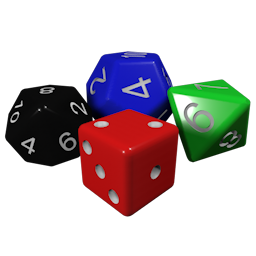
\includegraphics[width=0.25\linewidth]{Figures/dice_256x256.png}
}~
\subfloat[]{
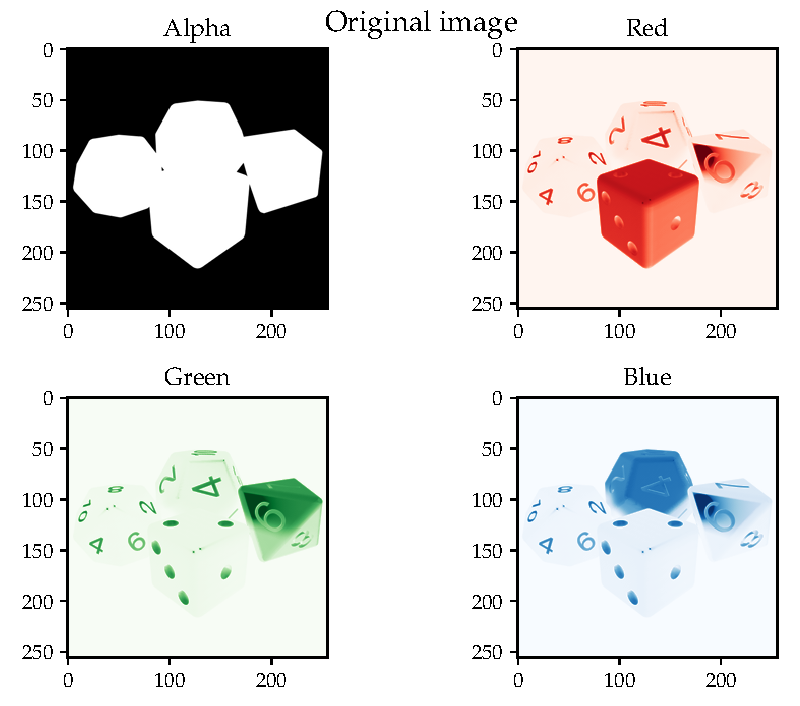
\includegraphics[width=0.355\linewidth]{Figures/dice_256x256_layers.pdf}
}~
\subfloat[]{
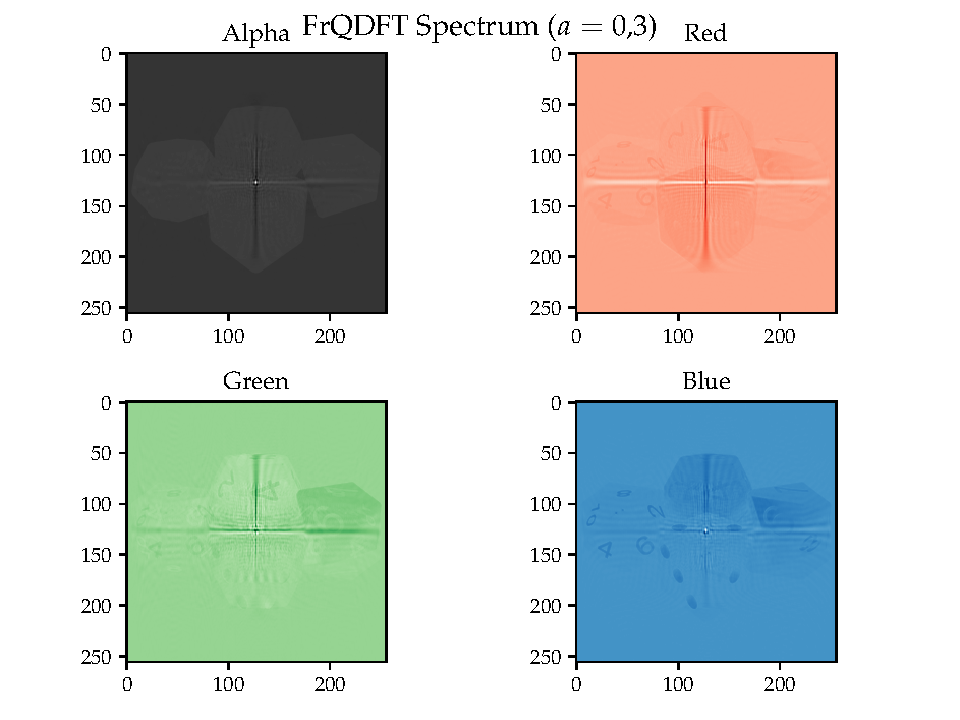
\includegraphics[width=0.355\linewidth]{Figures/dice_256x256_layers_frqdft.pdf}
}~
\floatsource
\end{figure*}

Once one is able to compute an orthogonal eigenbasis $ \mathbf{E} $ containing Hermite-Gaussian-like DFT eigenvectors, for instance by means of the generating matrix method, Theorem \ref{th:01} assures that matrix $ \mathbf{E} $ is also an eigenvector matrix for the QDFT. As a consequence, the transform matrix $ \mathbf{F} $ may be decomposed and written as
\begin{equation}
\label{eq:QDFTmtx}
\mathbf{F} = \mathbf{E} \mathbf{\Gamma} \mathbf{E}^T,
\end{equation}
in which the diagonal matrix $ \mathbf{\Gamma} $ is obtained by replacing $ \qi $ with $ \qmu $ in $ \mathbf{\Lambda} $ (Table \ref{tab:01}). Therefore, the \textit{fractional} quaternion Fourier transform, or simply FrQDFT, is obtained by raising each eigenvalue in $ \mathbf{\Gamma} $ to a so-called fractional order $ a \in \mathbb{R} $, so that
\begin{equation}
\label{eq:QDFTmtxa2}
\text{FrQDFT}_a\{ \mathbf{v} \} \overset{\Delta}{=} \mathbf{F}^a \mathbf{v},
\end{equation}
%\ref{eq:QDFTmtx}
where
\begin{equation}
\label{eq:QDFTmtxa}
\mathbf{F}^a = \mathbf{E} \mathbf{\Gamma}^a \mathbf{E}^T.
\end{equation}

The FrQDFT, as defined in (\ref{eq:QDFTmtxa2}) and (\ref{eq:QDFTmtxa}), possesses all the classical properties of a fractional Fourier transform:

\begin{itemize}
\item \textit{Reduction to the ordinary quaternion transform}: if $ a=1 $, then the synthesis equation in (\ref{eq:QDFTmtxa2}) equals (\ref{eq:QDFT}), coinciding with the QDFT. The proof is imediate.

\item \textit{Reduction to the identity}: if $ a=0 $, the FrQDFT reduces to the identity operator, represented as $ \mathbb{I} $.

\begin{proof}
From the orthogonality of the eigenvector matrix $ \mathbf{E} $,
\begin{equation}
%\label{key}
\mathbf{F}^0 = \mathbf{E} \mathbf{\Gamma}^0 \mathbf{E}^T = \mathbf{E} \mathbf{E}^T = \mathbb{I}.
\end{equation}
\end{proof}

\item \textit{Index addititivy}: applying the FrQDFT twice, using $ a $ and $ b $ as fractional orders, equals applying a single FrQDFT with fractional order $ a+b $. Equivalently, $ \mathbf{F}^a \mathbf{F}^b = \mathbf{F}^{a+b} $.

\begin{proof}
\begin{equation}
%\label{key}
\begin{aligned}
\mathbf{F}^a \mathbf{F}^b &= \mathbf{E} \mathbf{\Gamma}^a \mathbf{E}^T
\mathbf{E} \mathbf{\Gamma}^b \mathbf{E}^T \\
&= \mathbf{E} \mathbf{\Gamma}^a \mathbf{\Gamma}^b \mathbf{E}^T,
\end{aligned}
\end{equation}
but, since $ \mathbf{\Gamma} $ is a diagonal matrix, $ \mathbf{\Gamma}^a \mathbf{\Gamma}^b =
\mathbf{\Gamma}^{a+b} $, hence
\begin{equation}
%\label{key}
\mathbf{F}^a \mathbf{F}^b = \mathbf{E} \mathbf{\Gamma}^a \mathbf{\Gamma}^b \mathbf{E}^T = \mathbf{E} \mathbf{\Gamma}^{a+b} \mathbf{E}^T =
\mathbf{F}^{a+b}.
\end{equation}
\end{proof}

\item \textit{Unitary matrix}: the matrix $ \mathbf{F}^a $ is unitary, i.~e.
\begin{equation}
%\label{key}
\mathbf{F}^a (\mathbf{F}^a)^H = \mathbb{I},
\end{equation}
in which $ (\cdot)^H $ denotes the Hermitian (conjugate transpose) operator.
%\footnote{The \textit{quaternion} conjugation is considered, i.~e., se $ q = a + b\qi + c\qj + d\qk = r \exp (\qmu \theta) $, ent\~ao seu conjugado \'e $ \bar{q} = a - b\qi - c\qj - d\qk = r \exp (-\qmu \theta) $}

\begin{proof}
Since all FrQDFT eigenvalues $ \gamma_n $ are fourth roots of unity in the 1-$\qmu $ plane (i.~e., $ \gamma_n = \pm 1, \pm \qmu $ and, therefore, it has unit module), they can be written as $ \gamma_n = \exp \qmu \theta $ (in which $ \theta = 0, \pm \frac{\pi}{2}, \pi $). Hence
% ent\~ao podem ser escritos na forma $ \gamma_n = \exp \qmu \theta $ (em que $ \theta = 0, \pm \frac{\pi}{2}, \pi $). Assim,
\begin{equation}
%\label{key}
\overline{\gamma^a_n} = \gamma_n = \exp (-a \qmu \theta) = \gamma^{-a}_n,
\end{equation}
consequently
\begin{equation}
\label{eq:24}
(\mathbf{\Gamma}^a)^H = \mathbf{\Gamma}^{-a}.
\end{equation}

From (\ref{eq:24}) and (\ref{eq:QDFTmtxa}),
\begin{equation}
%\label{key}
\begin{aligned}
%\label{key}
(\mathbf{F}^a)^H &=  \left((\mathbf{E} \mathbf{\Gamma}^a) \mathbf{E}^T \right)^H =  \mathbf{E} \left(\mathbf{E} \mathbf{\Gamma}^a  \right)^H =
\mathbf{E} (\mathbf{\Gamma}^{a})^H \mathbf{E}^T = \mathbf{E} \mathbf{\Gamma}^{-a} \mathbf{E}^T = \mathbf{F}^{-a},
\end{aligned}
\end{equation}
and, following the index additivity and the reduction to identity properties,
\begin{equation}
%\label{key}
\begin{aligned}
%\label{key}
\mathbf{F}^a (\mathbf{F}^a)^H = \mathbf{F}^a \mathbf{F}^{-a} = \mathbf{F}^0= \mathbb{I}.
\end{aligned}
\end{equation}
\end{proof}
\end{itemize}

Before proceeding, it matters to notice that other approaches have been used to define fractional transforms especially suited for image encryption. Lima \textit{et al.} \cite{figueiredo2018} applied the generating matrix method to obtain eigenvectors --- in a fashion similar to this work --- and define multiorder reality-preserving discrete fractional transforms. Roopkumar \cite{roopkumar2016quaternionic}, on the other hand, defined a {continuous} one-dimensional quaternion fractional Fourier transform by using a reasoning similar to the symplectic decomposition of quaternions: adding together two traditional fractional Fourier operators with certain imaginary unit, with one of them multiplied by an orthogonal pure quaternion. None of the approaches, to the best of the author's knowledge, made use of eigenstructure analysis to define the FrQDFT and prove some of its properties.

\section{The multiparametric FrQDFT with application to color image encryption}
\label{sec:multi}
Frequently, fractional transforms are employed in both grayscale \cite{tao2010image} and color image \cite{kang2018reality, kang2018color} encryption. By setting the secret key to be the transform fractional order, alongside the use of multiple encryption or multiparametric transforms, one is able to create ciphers with sufficiently large key spaces and highly sensible to small key changes. This section presents an illustrative application of the FrQDFT, creating a holistic encryption scheme for PNG images based on the proposition of a multiparametric FrQDFT.

The definition of the multiparametric FrQDFT, referred to as MFrQDFT, consists of employing a different fractional order for each eigenvalue in $ \mathbf{\Gamma} $. The vector of fractional orders is represented by $ \mathbf{a} = [a_0, a_1, \dots, a_{N-1}] $. The MFrQDFT of a column vector $ \mathbf{v} $ is
\begin{equation}
\label{eq:MFrQDFT}
\text{MFrQDFT}\{ \mathbf{v} \} = \mathbf{E} \mathbf{\Gamma^a} \mathbf{E}^T \mathbf{v} = \mathbf{F^a} \mathbf{v}.
\end{equation}

The symbols $ \mathbf{\Gamma^a} $ and $ \mathbf{F^a} $ in (\ref{eq:MFrQDFT}) are abuses of notation. One must comprehend $ \mathbf{\Gamma^a} $ as the diagonal matrix obtained after raising the $ n $-th entry in the diagonal of $ \mathbf{\Gamma} $ to the $ n $-th component in $ \mathbf{a} $. On the other hand, $ \mathbf{F^a} $ indicates the matrix $ \mathbf{E} \mathbf{\Gamma^a} \mathbf{E}^T $. As it was done in Subsection \ref{subsec:2D_QDFT}, the 2D-MFrQDFT of a quaternion matrix $ \mathbf{X} $, e.~g. representing a PNG matrix, is written as
\begin{equation}
\label{eq:2DMFrQDFT}
\text{2D-MFrQDFT}\{\mathbf{X} \} \overset{\Delta}{=} \mathbf{\widehat{X}} = \mathbf{F^a} \mathbf{X} \mathbf{F^a}^T,
\end{equation}
with inverse transform obtained from the properties listed in Section \ref{sec:FrQDFT}
\begin{equation}
\label{eq:2DMFrQDFTinv}
\text{2D-MFrQDFT}^{-1}\{ \mathbf{\widehat{X}} \} = (\mathbf{F^a}^H) \mathbf{\widehat{X}} (\overline{\mathbf{F^a}}).
\end{equation}

\begin{figure*}
\centering
\caption{Proposed encryption scheme, exploring the 2D-MFrQDFT.}
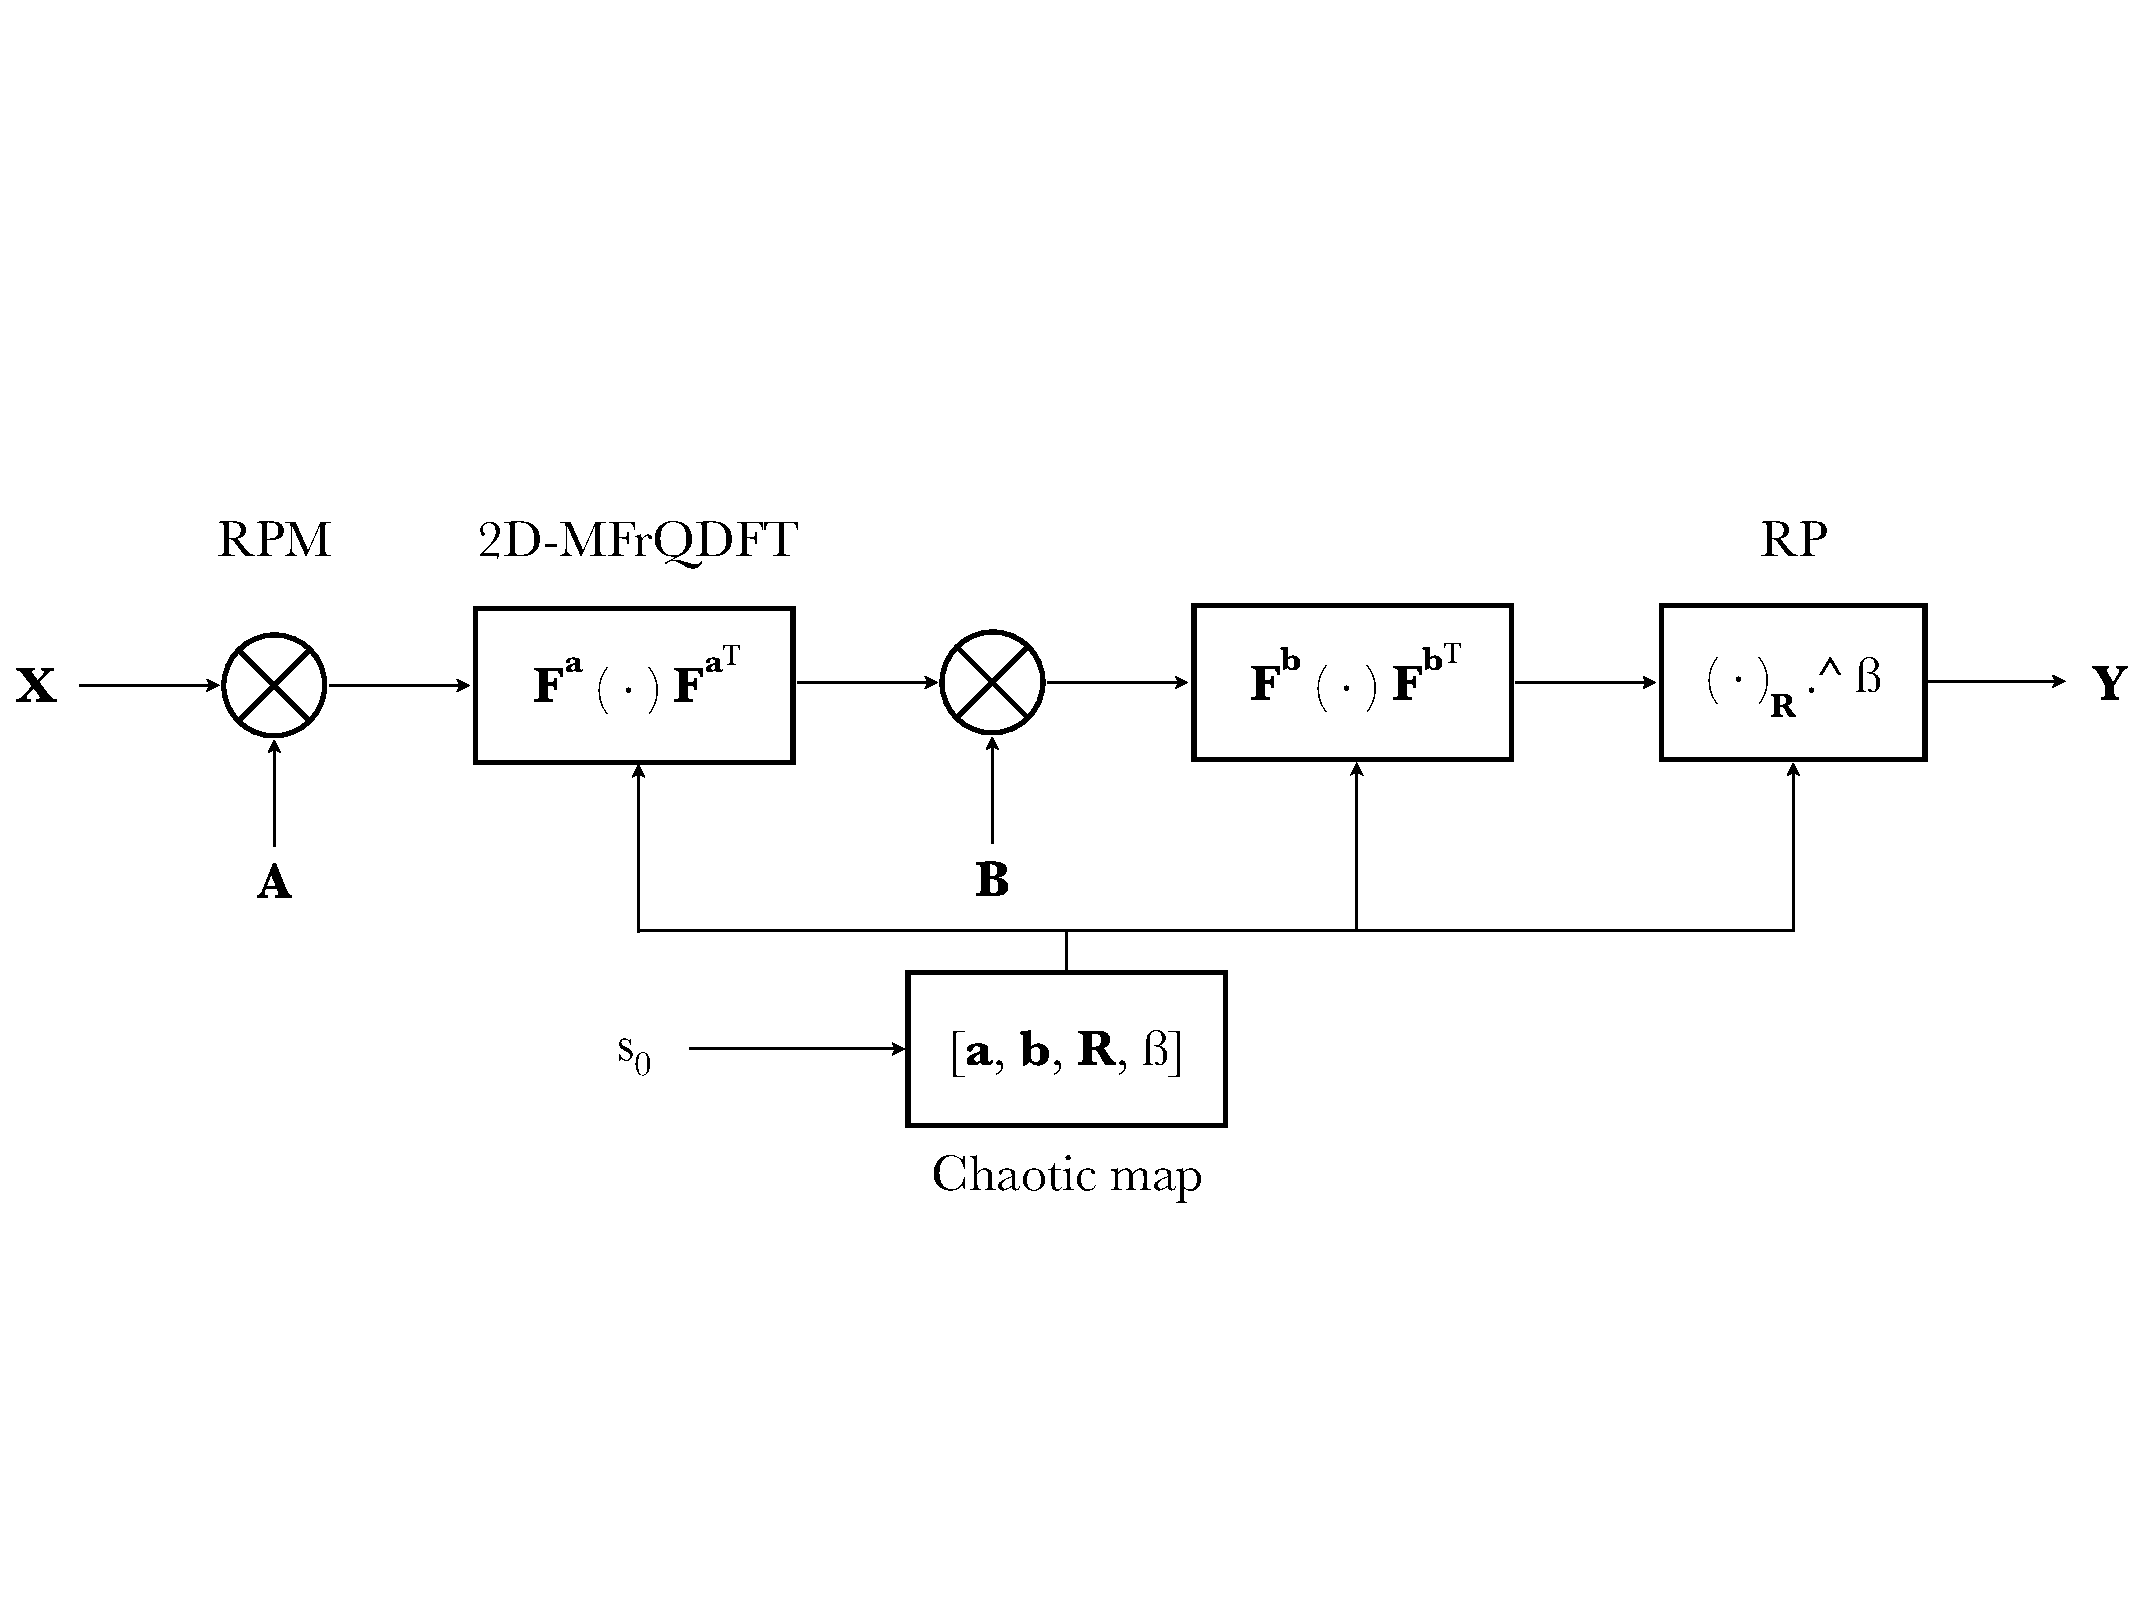
\includegraphics[width=0.9\linewidth]{Figures/esquema_EN.pdf}
\floatsource
\label{fig:cifragem}
\end{figure*}

\begin{figure*}
\centering
\caption{(a) Encrypted image. (b) Image decrypted with the correct key $ s_0 $. (c) Image decrypted with the wrong key $ \widetilde{s_0} = s_0 + \epsilon $, with $ \epsilon = -1{,}6 \cdot 10^{-80} $.}
\subfloat[\label{fig:ciphered01}]{

\includegraphics[width=0.2\linewidth]{Figures/sage_Encrypted_image.png}
}~
\subfloat[\label{fig:ciphered02}]{
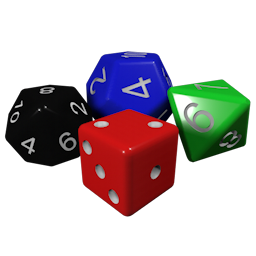
\includegraphics[width=0.25\linewidth]{Figures/Decrypted_image_error_0.png}
}~
\subfloat[\label{fig:ciphered03}]{

\includegraphics[width=0.2\linewidth]{Figures/sage_Decrypted_image_error_minus1dot6.png}
}~
\floatsource
\end{figure*}

\subsection{Encryption scheme using MFrQDFT}

The chosen implementation for the PNG image encryption algorithm mixed a block of random-phase modulation (RPM, also called phase mask in \cite{chen2018multiple} and \cite{singh2008optical}) and multiparametric transform. As suggested by \cite{hsue2018enhancing}, a non-linear step of random power is also used. Fig. \ref{fig:cifragem} depicts the system building blocks.

The plaintext image is initially converted into a quaternion matrix $ \mathbf{X} $, which is input to a 2-round processing with RPM $ + $ 2D-MFrQDFT. The random-phase modulation consists of element-wise multiplication by a matrix of random unit quaternions. This role is fulfilled by matrices $ \mathbf{A} $ and $ \mathbf{B} $ in Fig. \ref{fig:cifragem}. The \textit{inverse} RPM (in decryption) is achieved using the \textit{conjugate} of the matrix used during encryption.

The random-power block (RP) is the final step in the encryption method. It creates non-linearity by raising randomly selected entries of the matrix $ \mathbf{X} $ to a random parameter $ \beta \in \ ]0,1[$. This selection is performed by a binary matrix $ \mathbf{R} $, so that the output of the RP block to an input quaternions matrix $ \mathbf{M} $ is
\begin{equation}
%\label{key}
\text{RP}(\mathbf{M})_{i,j} =
\begin{cases}
(\mathbf{M}_{i,j})^\beta & \text{if } \mathbf{R}_{i,j} = 1, \\
\mathbf{M}_{i,j} & \text{if } \mathbf{R}_{i,j} = 0.
\end{cases}
\end{equation}
During decryption, one must use the same matrix $ \mathbf{R} $ and an exponent $ \beta^{-1} $.

A chaotic map was used to generate a pseudorandom sequence $ \mathbf{s} $ of numbers between 0 and 1, from which all of the encryption parameters were drawn: the fractional order vectors $ \mathbf{a} $ and $ \mathbf{b} $ of the two 2D-MFrQDFTs, the parameter $ \beta $ and the matrix $ \mathbf{R} $\footnote{For each entry $ \mathbf{R}_{i,j} $, a corresponding element $ s_k $ of $ \mathbf{s} $ was taken and $ \mathbf{R}_{i,j} $ was set to 1 if and only if $ s_k > 0{,}5 $, $ \mathbf{R}_{i,j} = 0 $ otherwise.} for the RP block. The random-phase modulation matrices were produced beforehand and could be left public in the scheme documentation. The encryption of a $ 256 \times 256 $-pixels image, therefore, requires a sequence of length $ 256 + 256 + 256^2 + 1  $. The secret key consists of the seed $ s_0 $ of the chaotic map, a floating point variable between 0 and 1.
%It is clear how the key space and the scheme security depend on the seed floating-point precision and the chosen chaotic map randomness.
As a consequence, the key space is determined by the smallest deviation $ \epsilon $ from $ s_0 $ so that, using the wrong key $ \widetilde{s_0} = s_0 \pm \epsilon $ in decryption, it still leads to a noisy image without any detectable trace of original information.

The key space dimension, denoted by $ [K] $, is the ratio between the range of all possible keys and the range of wrong keys \textit{which still lead to partial image reconstruction}. The latter is $ [s_0 - \epsilon, s_0 + \epsilon] $, following the previous definition of $ \epsilon $. Since $ s_0 \in \ ]0,1[ $,
\begin{equation}
%\label{key}
[K] = \frac{1 - 0}{s_0 + \epsilon - (s_0 - \epsilon)} = \frac{1}{2 \epsilon}.
\end{equation}

When testing the encryption scheme, the \textit{tent map} \cite{singh2008optical} was chosen as tool for generating the $ \mathbf{s} $ sequence; it is recursively defined as
\begin{equation}
%\label{key}
s_{n+1} =
\begin{cases}
\gamma s_n & \text{if } 0 \leq s_0 < 0{.}5, \\
\gamma(1 - s_n) & \text{if } 0{.}5 \leq s_0 \leq 1.
\end{cases}
\end{equation}
with $0 <  \gamma \leq 2 $.

The tent map parameters were set to $ s_0 = 0{.}3 $ and $ \gamma = 1{.}8 $, for no particular reason other than obeying the range of values for chaotic behavior. The proposed encryption algorithm was used on the image in Fig. \ref{fig:dice}, what yielded the ciphered output in Fig. \ref{fig:ciphered01}.

In order to evaluate the key space dimension, the ciphered image was decrypted using keys $ \widetilde{s_0} = s_0 \pm \epsilon $ for different values of $ \epsilon \in [-10 \times 10^{-80}; 10 \times 10^{-80}]$, with the aid of multiple precision tools provided by the \textit{RealField} class in the SageMath software. By the end of each decryption, it was computed the MSE between the supposedly recovered image and the original one, what is plotted in Fig. \ref{fig:MSE}. The graph does not change smoothly because each tweak in $ s_0 $ propagates along the whole sequence $ \mathbf{s} $, what affects randomly all the decryption parameters. This is, of course, consequence of the nature of a chaotic map. As shown in the graph, the smallest MSE (still using wrong keys, with $ \epsilon \neq 0 $) was 39dB, obtained with $ \epsilon = -1{,}6 \times 10^{-80} $.

Fig. \ref{fig:ciphered02} and \ref{fig:ciphered03} show the decrypted images using $ \epsilon = 0 $ and $ \epsilon = -1{,}6 \times 10^{-80} $, respectively. It can be seen that the wrong key which caused the smallest MSE still produced a seemingly random PNG image, a desirable property for an encryption scheme. Since the smallest deviation used in this test was $ 0{,}83 \times 10^{-80} $, it follows that the key space dimension is, at least, equal to
\begin{equation}
%\label{key}
[K] = \frac{1}{2 \times 0{,}83 \times 10^{-80}} \approx 6{,}0 \times 10^{79},
\end{equation}
what means the key length must be
%o que significa que cada chave deve ter comprimento de
\begin{equation}
%\label{key}
\lceil 79 \log_2 10 \rceil = 263\text{ bits},
\end{equation}
a value greater than 256 bits, assumed to be appropriate for symmetric encryption schemes, by information security reports such as ECRYPT \cite{smart2018algorithms}. It is also clear from these computations and Fig. \ref{fig:ciphered03} how sensitive the scheme is to small key changes: the smallest modification within the precision of $ 10^{-80} $ in the seed $ s_0 $ was enough to provide a completely noisy decrypted image (cf. Fig. \ref{fig:ciphered03}). The high key sensitivity is also indicated by the sharp dip in the MSE $\times $ Error graph in Fig. \ref{fig:MSE}.
%, \'e um tamanho de chaves apropriado para manter sistemas de cifra sim\'etrica em uso por um per\'iodo estimado de 30 a 50 anos.
%.
%
%%A Fig. \ref{fig:RPM} ilustra a oculta\c c\~ao gradual de informa\c c\~ao visual, ao menos nos pixels n\~ao-nulos, ap\'os cada itera\c c\~ao do bloco de RPM. A cada itera\c c\~ao, uma matriz aleat\'oria diferente \'e usada.
%
\begin{figure}
\centering
\caption{Mean squared error, in dB, between the original and the decrypted images as function of the key error $ \epsilon $.}
\includegraphics[width=10cm]{Figures/MSEdb_FrQDFT_EN.pdf}
\floatsource
\label{fig:MSE}
\end{figure}
%

Such an encryption scheme would not only be safe against brute-force attacks, given its key space dimension, but also known-plaintext attack. The reason for this is the non-linearity provided by the random-power block, as argued intensely by Hsue \cite{hsue2018enhancing}. Resistance to chosen-plaintext attacks, however, is not guaranteed, although simple adjustments could be done in future works to address this problem: the vector of fractional orders $ \mathbf{a} = \{ a_0, a_1, \dots, a_{N-1} \} $ could be made dependent on both the plain image and external parameters (such as the secret seed $ s_0 $). Such tweak in the algorithm would block the extraction of information from comparing chosen plain images with their encrypted counterparts \cite{chai2019color, hu2017chaotic, murugan2016image}, making the scheme resistant to chosen-plaintext and chosen-ciphertext attacks \cite{wang2012novel}; with resistance also to the weaker attacks of brute-force and known-plaintext.

Alongside the investigation of key space dimension and sensitivity, histogram analysis play an important role in describing the performance of encryption schemes. A practical cipher should present an output symbol distribution ideally independent from the cleartext, so that no information is leaked through histogram visualization  \cite{zhang2014symmetric}.
% "An ideal encrypted image should have a
% uniform and completely different histogram against the plain-image for preventing the adversary from extracting any mean-
% ingful information from the fluctuating histogram of the cipher-image." (zhang2014symmetric)
In the case of a PNG image, four histograms are drawn, one for each layer. Fig. \ref{fig:testing_hist} depicts a test PNG image split into its color and opacity components and the corresponding histograms, both prior and after encryption. A group of 13 $ 256\times 256 $-pixels PNG images were encrypted using the proposed method and the histograms of the ciphered output were collected, what is shown in Fig. \ref{fig:allhistograms}. No matter how diverse the input images may be, the histograms present continuously the same profile, what indicates decoupling of information between plain and ciphered images. Although a deeper study on the properties and safety standards of the proposed encryption scheme is needed for full description of its capacity, the analysis presented fit in the scope of this work and fulfill the goal of presenting the MFrQDFT with a clear and illustrative application.
%{\color{blue}Each image was ciphered using one of the following randomly defined keys (IMPLEMENTAR): $s_0 = $}. % For quantity analyses of each key, we employ variances of histograms to evaluate uniformity of ciphered images. The low-
% er value of variances indicates the higher uniformity of ciphered images. We also calculate the two variances of ciphered
% images which are encrypted by different secret keys on the same plaintext image. The closer of the two values of variances
% indicates the higher uniformity of ciphered images when the secret keys are varying. The variance of histograms is presented
% as follows:

%Histogram analysis: point out that the conversion from float to int, used prior to histogram-making, did not incur in information loss, because the MSE between the original image and the decrypted, AFTER CONVERSION, was
%MSE:  7.380345314385882e-25
%MSEint:  7.380345314385882e-25


\newcommand{\constlength}{0.5}

\begin{figure}[htbp]
\centering
\caption{(a) Test image in PNG format, with 256$ \times $256 pixels. (b) Color and opacity layers of the \textit{decrypted} image (which coincides with the original in (a)). (c) Histograms of each layer of the \textit{decrypted} image. (d) Encrypted image, in PNG format. (e) Color and opacity layers of the \textit{encrypted} image. (f) Histograms of each layer of the \textit{encrypted} image.}
\subfloat[]{\includegraphics[width=0.35\linewidth]{Figures/alphatest_resized_decrypted.png}}~
\subfloat[]{\includegraphics[width=\constlength\linewidth]{Figures/alphatest_resized_decrypted_RGBA_layers.pdf}} \\
\subfloat[]{\includegraphics[width=\constlength\linewidth]{Figures/alphatest_resizeddecrypted_histograms.pdf}}~
\subfloat[]{\includegraphics[width=0.3\linewidth]{Figures/alphatest_resized_encrypted_img.png}} \\
\subfloat[]{\includegraphics[width=\constlength\linewidth]{Figures/alphatest_resized_encrypted_RGBA_layers.pdf}}~
\subfloat[]{\includegraphics[width=\constlength\linewidth]{Figures/alphatest_resized_encrypted_histograms.pdf}}
\floatsource[all images were generated by the author, except the first in (a), which was taken from the World Wide Web Consortium website at \texttt{\url{https://www.w3.org/Graphics/PNG/Alphatest.html}}]
\label{fig:testing_hist}
\end{figure}

\newcommand{\fixedlength}{0.35}
\newcommand{\smallerlength}{0.15}
\begin{figure}[htbp]
\centering
\caption{Set of 13 PNG test images, 256$ \times $256 pixels, alongside the histograms of each layer (colors and opacity) of their encrypted version.}
\subfloat[]{\includegraphics[width=\smallerlength\linewidth]{Figures/dice_256x256_decrypted.png}}~
\subfloat[]{\includegraphics[width=\fixedlength\linewidth]{Figures/dice_256x256_encrypted_histograms.pdf}}~
\subfloat[]{\includegraphics[width=\smallerlength\linewidth]{Figures/another_dice_resized_decrypted.png}}~
\subfloat[]{\includegraphics[width=\fixedlength\linewidth]{Figures/another_dice_resized_encrypted_histograms.pdf}}\\
\subfloat[]{\includegraphics[width=\smallerlength\linewidth]{Figures/candle_resized.png}}~
\subfloat[]{\includegraphics[width=\fixedlength\linewidth]{Figures/candle_encrypted_histograms.pdf}}~
\subfloat[]{\includegraphics[width=\smallerlength\linewidth]{Figures/pipe_resized.png}}~
\subfloat[]{\includegraphics[width=\fixedlength\linewidth]{Figures/pipe_encrypted_histograms.pdf}}\\
\subfloat[]{\includegraphics[width=\smallerlength\linewidth]{Figures/dog_resized.png}}~
\subfloat[]{\includegraphics[width=\fixedlength\linewidth]{Figures/dog_encrypted_histograms.pdf}}~
\subfloat[]{\includegraphics[width=\smallerlength\linewidth]{Figures/parrot_resized.png}}~
\subfloat[]{\includegraphics[width=\fixedlength\linewidth]{Figures/parrot_encrypted_histograms.pdf}}\\
\subfloat[]{\includegraphics[width=\smallerlength\linewidth]{Figures/colorparrots_resized.png}}~
\subfloat[]{\includegraphics[width=\fixedlength\linewidth]{Figures/colorparrots_encrypted_histograms.pdf}}~
\subfloat[]{\includegraphics[width=\smallerlength\linewidth]{Figures/bouquet_resized.png}}~
\subfloat[]{\includegraphics[width=\fixedlength\linewidth]{Figures/bouquet_encrypted_histograms.pdf}}

\vspace{3em}
\noindent \textit{(The figure continues on the next page).}
\label{fig:allhistograms}
%\caption{Legenda.}
\end{figure}

\stepcounter{figure}
\begin{figure}[htbp]
\centering
\ContinuedFloat
\subfloat[]{\includegraphics[width=\smallerlength\linewidth]{Figures/switzerland_resized.png}}~
\subfloat[]{\includegraphics[width=\fixedlength\linewidth]{Figures/switzerland_encrypted_histograms.pdf}}~
\subfloat[]{\includegraphics[width=\smallerlength\linewidth]{Figures/london_resized.png}}~
\subfloat[]{\includegraphics[width=\fixedlength\linewidth]{Figures/london_encrypted_histograms.pdf}}\\
\subfloat[]{\includegraphics[width=\smallerlength\linewidth]{Figures/russia_resized.png}}~
\subfloat[]{\includegraphics[width=\fixedlength\linewidth]{Figures/russia_encrypted_histograms.pdf}}~
\subfloat[]{\includegraphics[width=\smallerlength\linewidth]{Figures/globe_resized.png}}~
\subfloat[]{\includegraphics[width=\fixedlength\linewidth]{Figures/globe_encrypted_histograms.pdf}}\\
\subfloat[]{\includegraphics[width=\smallerlength\linewidth]{Figures/phones_resized.png}}~
\subfloat[]{\includegraphics[width=\fixedlength\linewidth]{Figures/phones_encrypted_histograms.pdf}}
\floatsource[plots generated by the author, whereas the test images were taken from the PurePNG online free database, available at \texttt{\url{https://purepng.com/}}, under CC0 license]
\end{figure}

Finally, as stated at the beginning of the chapter, there are a multitude of studies on image encryption, each addressing particular aspects and problems. Therefore, it is adequate to acknowledge the position of this proposed encryption algorithm in the literature landscape. Without providing an extensive and complete analysis, for lack of space, some remarks can be done. The key space dimension in related works vary from circa $ 10^{54} $, around 160 bits, in a work by Wang \textit{et al.} with flexible key space \cite{wang2015novel}, to more than 400 bits, in a paper by Zhang \textit{et al.} \cite{zhang2015new}, an interval which includes the 260 bits of the proposed algorithm. Regarding time of encryption, Wang \textit{et al.} \cite{wang2015novelchaotic} used Arnold cat map and dynamic random growth to obtain large running speed of the encryption and decryption algorithm. This is an aspect our proposed scheme is not optimized for, although great improvement in processing time can be achieved if the eigenvector and eigenvalue matrices of the QDFT are stored in-memory, taking the eigendecomposition out of the encryption process. As a final comment, the main advantages of the proposed scheme are its modularization, the holistic processing of color images with opacity layer, the lack of long iterations and the ease to describe, comprehend and implement.

\section{Concluding remarks}
\label{sec:conclusao}
This chapter investigated the eigenstructure of the quaternion discrete Fourier transform. Although quaternion matrix decomposition is a challenging topic, the problem for the QDFT was solved by proving that this transform and the DFT share symmetric eigenvectors, what allowed for the construction of an orthogonal eigenbasis of the QDFT, using Hermite--Gaussian-like DFT eigenvectors \cite{de2017discrete}. This result led to the definition of a fractional QDFT, which was proven to hold properties similar to those of the FrDFT, its complex-valued counterpart.

The FrQDFT was further generalized by introducing the MFrQDFT, a multiparametric version. Exploring the 4D nature of quaternions, a holistic encryption scheme for color images with opacity layer was proposed, as an illustrative application of the 2D-MFrQDFT, and shown to provide satisfactorily large key space and key sensitivity, resistance to known-plaintext attack and ease of description and implementation. Future works could possibly expand this analysis and address whether some hypercomplex image moments, such as ternary radial harmonic Fourier moments and quaternion polar harmonic \cite{wang2019ternary,wang2018quaternion}, could be used for image encryption, eventually in specific scenarios and applications.

\chapter{Quaternion graph signal processing}
\label{ch:QGSP}

Graph signal processing is a highly flexible tool for analysing and transforming graph-based data. However, as it happens with so many engineering tasks, often it appears to mix mathematics and art: the experienced GSP user knows that quite a few characteristics of the underlying graph are open to be determined by the very problem at hand and by the user's intuition. That is, whether one must consider real or complex edge weights, directed or undirected graphs, whether loops or multiple edges shall be allowed, all of these modeling choices arise from the data and from the way one considers the most appropriate to represent the relations within. We make hereby the argument that changing the algebra over which the graph signal samples (and edge weights) are defined, although rarely regarded among modeling choices, may reveal powerful new tools.

Let us take an example of how the signal algebra may affect the processing possibilities, in the current state of GSP. Undirected graphs with real-valued weights are a common option for those used to model data defined over geographic spaces, since it is reasonable to consider the adjacency relations to be non-directional and weighted by positive real numbers \parencite{shuman2013emerging}. However, the same topology would be arguably inappropriate should one deal with complex-valued signals: a directed graph or a graph with complex-valued edge weights would be more reasonable options to evaluate, since they would produce graph Fourier transform matrices with complex entries. Although this scenario may seem to lack practical purpose, defining a graph signal with samples lying in extensions of the real field (e.g. complex numbers) would be justified by the increase in the amount of information stored within each sample (from a single real number, to twice as much in the complex case).

Electrical engineers for many decades have exploited the benefits of handling more than one real-valued information (e.g. magnitude and phase) encoded in a single signal sample, and a similar motivation led to Sangwine's \parencite{sangwine1996fourier} discrete version of a family of bidimensional transforms over the \textit{quaternions} (a skew-field which extends the complex numbers by having four real valued components). As the reader may recall from Chapter \ref{ch:Intro}, these transforms used this class of hypercomplex numbers to perform holistic color image processing, handling all three color channels at once. In fact, \emph{quaternion signal processing} was created to embed three- or four-dimensional data into one-dimensional signals \parencite{took2008quaternion}. Ever since, quaternion transforms have been employed not only on color image processing \parencite{ell2007hypercomplex,chen2018quaternion,li2013quaternion,evans2000hypercomplex}, but also on other tasks such as bivariate signal analysis \parencite{flamant2017spectral,flamant2017time,flamant2018complete}.

In Chapter \ref{ch:reviewGSP} it was presented the motivation and fundamentals of graph signal processing, while Chapter \ref{ch:FrGSO} delved into the exploration of a fractional graph shift.
This chapter attempts to further extend the borders of GSP by pondering the problem of signal processing on graphs with quaternion-valued edge weights, referred to as \textit{quaternion graph signal processing}.

\section{Laying the foundations for QGSP}

Since QGSP is the development and application of GSP tools to the context of quaternion-valued signals and graph edge weights, it starts by extending the usual definition of graph signal in (\ref{eq:def_signal}), replacing the complex-valued numbers with quaternions. As such, the quaternion graph signal $\mathbf{s}$, defined over the graph $\mathcal{G} = \{\mathcal{V}, \mathbf{A}\}  \ | \ \mathbf{A} \in \mathbb{H}^{n \times n}$, is defined as
\begin{equation}\label{eq:qgsp_defs}
    s: \ \mathcal{V} \rightarrow \mathbb{H} \ | \ s(v_i) = s_i.
\end{equation}

This definition unfolds some challenges: what does it
mean to have a smooth quaternion graph signal? Does the well known benefit of quaternion signal processing, namely holistic manipulation of multiple channels of information, transfer to graph signal processing? How is one able to design LSI filters in QGSP?

In order to properly address these questions and establish the foundations of QGSP, a few milestones were set to be conquered. Firstly, an algorithm to compute the direct and inverse (quaternion) graph Fourier transforms should be proposed, to allow for basic spectral analysis. This includes revisiting the definition of frequency ordering, which is well understood only for real and complex graph signals. Secondly, QGSP should ideally provide a class of graphs for which the Fourier transform is known to exist (and hopefully easier to compute than outside this class). The reasoning here is to find a case similar to that of usual GSP, where it is known that undirected graphs with real-valued edge weights always have diagonalizable GSOs. Finally, QGSP should ideally provide a method to design graph FIR filters, tailored to approximate a given frequency response. The Subsection \ref{subsec:eigendecomposition} gives the first step towards QGSP, properly defining the QGFT and studying the eigendecomposition of the quaternion graph shift operator (QGSO).

\subsection{Eigendecomposing the shift operator}
\label{subsec:eigendecomposition}
At the very center of vertex-frequency analysis in GSP lies the definition that a basis of eigenvectors of the chosen graph shift operator act as Fourier components for the space of graph signals. This can be directly translated to QGSP, after taking into account the results presented in Chapter \ref{ch:reviewQuat}, regarding diagonalization of quaternion matrices.

\begin{definition}
    Given the graph $\mathcal{G} = \{\mathcal{V}, \mathbf{A}\}  $,  with adjacency matrix $ \mathbf{A} \in \mathbb{H}^{n \times n}$, the \textit{quaternion graph Fourier transform} (QGFT) is the projection of a graph signal onto the eigenspace of $\mathbf{A}$.
\end{definition}

The first step towards the QGFT is, therefore, the generation of a basis of (possibly generalized) eigenvectors of the adjacency matrix. This work has dealt only with the case of diagonalizable graph matrices, but the use of the Jordan canonical form can be investigated for non-diagonalizable QGSOs \parencite{Longxuan1996}.

On the one hand, from the Corollary \ref{cor:diagonalizable} it is known that the diagonalizability of an adjacency matrix $\mathbf{A}$ both implies and requires that of its complex adjoint matrix $\rchi_A$. Let us write $\mathbf{A} = \mathbf{V} \mathbf{\Lambda} \mathbf{V}^{-1}$. On the other hand, Theorem \ref{th:02} guarantees that the eigenvalues of the adjacency matrix can be taken as half the ones of its complex adjoint matrix. More specifically, they can be taken as the union of the set of eigenvalues with positive imaginary part (recall that they are complex-valued) and the set of \textit{distinct} eigenvalues with null imaginary part (recall that every real-valued eigenvalue appears twice).

However, once the desired eigenvalues from $\rchi_A$ have been defined, how does one assemble $\mathbf{V}$ out of the eigenvectors of $\rchi_A$? That is answered by Equation (\ref{eq:eigvalueequation}), which is rewritten below for convenience:
\begin{equation*}
    \begin{pmatrix}
        \mathbf{A}_1              & \mathbf{A}_2            \\
        - \overline{\mathbf{A}}_2 & \overline{\mathbf{A}}_1
    \end{pmatrix}
    \begin{pmatrix}
        \mathbf{v}_1 \\
        - \overline{\mathbf{v}}_2
    \end{pmatrix} =
    \begin{pmatrix}
        \mathbf{v}_1 \\
        - \overline{\mathbf{v}}_2
    \end{pmatrix}
    \lambda.
\end{equation*}
On the left-hand side of the equation, we find $\rchi_A$ and one of its eigenvectors, which is written in terms of the symplectic decomposition of a quaternionic column vector $\mathbf{v} = \mathbf{v}_1 + \mathbf{v}_2 \qj$. As it turns out, $\mathbf{v}$ is precisely the eigenvector of $\mathbf{A}$ associated with the eigenvalue $\lambda$. This is proven in Appendix \ref{ch:AppendixA} and constitutes a minor contribution of this thesis. The answer to the question raised a few lines above, to sum up, is that once one has the chosen eigenvalues of $\rchi_A$, it is possible to assemble $\mathbf{V} \in \mathbb{H}^{n \times n}$ out of the respective eigenvectors of $\rchi_A$ by simply spliting these $2n$-long eigenvectors into halves: the first half corresponds to $\mathbf{v}_1$ (the simplex part of the eigenvector $\mathbf{v}$), while the second half is $- \overline{\mathbf{v}}_2$ (with $\mathbf{v}_2$ being the perplex part of $\mathbf{v}$).

So far we are able to obtain $\mathbf{V}$ from $\mathbf{A}$, bypassing the direct eigendecomposition of a quaternion matrix by using its complex adjoint. However, the question of how to get $\mathbf{V}^{-1}$, if it exists, poses itself imediately, after all $\mathbf{V}$ corresponds to the \textit{inverse} of the QGFT. Let us address this point.

\subsection{Inversion of the eigenvector matrix and frequency ordering}
\label{subsec:inversion}
The inversion of quaternion matrices is certainly a problem tackled by many researchers, but is not featured prominently in literature, at least not as far as the author is aware. There is, however, an algorithm proposed by \parencite{cohen1999quaternionic} during studies on the determinant of quaternion matrices, when they highlighted the utility of Schur complements on computing the inversion of any matrix $\mathbf{M} \in \mathcal{R}^{n \times n}$ over the ring $\mathcal{R}$. Let us go quickly through their idea. Given that $\mathbf{M}$ is written in block form,
\begin{equation}
    \label{eq:block}
    \mathbf{M} = \begin{pmatrix}
        \mathbf{A} & \mathbf{B} \\
        \mathbf{C} & \mathbf{D}
    \end{pmatrix},
\end{equation}
and under the requisite that $\mathbf{A} \in \mathcal{R}^{k \times k}$ is invertible, the Schur complement of $\mathbf{A}$ in $\mathbf{M}$ is defined as
\begin{equation}
    \mathbf{A}_s \overset{\Delta}{=} \mathbf{D}
    - \mathbf{C}\mathbf{A}^{-1} \mathbf{B}.
\end{equation}
Given that $\mathbf{A}_s$ is also invertible, the closed formula for the inverse of $\mathbf{M}$ is
\begin{equation}
    \label{eq:schur}
    \mathbf{M}^{-1} =
    \begin{pmatrix}
        \mathbf{I}_k & - \mathbf{A}^{-1} \mathbf{B} \\
        \mathbf{0}   & \mathbf{I}_{n - k}
    \end{pmatrix}
    \begin{pmatrix}
        \mathbf{A}^{-1} & \mathbf{0}        \\
        \mathbf{0}      & \mathbf{A}_s^{-1}
    \end{pmatrix}
    \begin{pmatrix}
        \mathbf{I}_k                 & \mathbf{0}         \\
        - \mathbf{C} \mathbf{A}^{-1} & \mathbf{I}_{n - k}
    \end{pmatrix},
\end{equation}
so that the inversion of $\mathbf{M}$ is now reduced to inversion of the two smaller matrices $\mathbf{A}$ and $\mathbf{A}_s$.

Although this method proposes a closed formula for quaternion matrix inversion, it requires an exhaustive search for a submatrix in the upper left corner that, simultaneously, is \textit{invertible} and \textit{has invertible Schur complement}. Probably the idea can be explored in the future and used to find an efficient way to compute $\mathbf{V}^{-1}$, but in Algorithm \ref{alg:qinv} we propose a more reasonable compromise between processing speed, implementation time and broad applicability.

The reasoning goes as follows. According to Theorem \ref{th:equiv02}, a necessary and sufficient condition for the invertibility of a matrix $\mathbf{V} \in \mathbb{H}^{n \times n}$ is the existance of $\rchi^{-1}_{V}$. Moreover, from Theorem \ref{th:equiv01}, if $\rchi^{-1}_{V}$ exists and has the form of a complex adjoint matrix, let us say $\rchi_{V}^{-1} = \rchi_{M}$, then it follows that $\mathbf{M} = \mathbf{V}^{-1}$, since the theorem guarantees that
\begin{equation}
    \rchi_{V} \rchi_{M} = \rchi_{V} \rchi_{V}^{-1} = \mathbf{I}_{2n \times 2n} = \rchi_{I_{n \times n}}
    \Rightarrow \mathbf{V} \mathbf{M} = \mathbf{I}_{n \times n},
\end{equation}
letting $\mathbf{I}_{m \times m}$ be the identity matrix of order $m$\footnote{For simplicity, this notation is slightly loose, representing both a complex- and a quaternion-valued identity matrix, since in both cases their entries have zero-valued or zero-normed imaginary parts.}. That is, once the complex adjoint of $\mathbf{V}$ is computed, one simply needs to compute its inverse, if it exists, and verify if it follows the format in Definition \ref{def:complexadjoint}.

\newcommand{\algorithmspacing}{0.5}
\begin{algorithm}
    \label{alg:qinv}
    Compute the inverse of a quaternion-valued matrix, if a sufficient condition for its existence is met:
    \vspace*{-\algorithmspacing\baselineskip}
    \begin{leftbar}
        \noindent\textbf{\upshape Input:} $\mathbf{V} \in \mathbb{H}^{n \times n}$. \textbf{\upshape Output:} $\mathbf{V}^{-1}$ or {\upshape None}.

        \begin{algorithmic}[1]
            \State $\rchi_V \gets \mathrm{to\_complex\_adjoint}(\mathbf{V})$
            \If{$\det(\rchi_V) = 0$}
            \State \Return {\upshape None}
            \Else
            \State $\mathbf{U} \gets \mathrm{inverse}(\rchi_V)$
            \If{$\mathbf{not} \ \mathrm{has\_complex\_adjoint\_form}(\mathbf{U})$}
            \State \Return {\upshape None}
            \Else
            \State $\mathbf{V}^{-1} \gets \mathrm{from\_complex\_adjoint}(\mathbf{U})$
            \State \Return $\mathbf{V}^{-1}$
            \EndIf
            \EndIf
        \end{algorithmic}
    \end{leftbar}
    \vspace*{-\algorithmspacing\baselineskip}
    \noindent These functions were used in the algorithm to improve readability:
    \vspace*{-\algorithmspacing\baselineskip}
    \begin{itemize}[noitemsep]
        \item $\mathrm{to\_complex\_adjoint}$: converts a quaternion matrix to its complex adjoint form.
        \item $\mathrm{from\_complex\_adjoint}$: converts a complex adjoint matrix to its quaternion-valued form.
        \item $\mathrm{inverse}$: computes the inverse of a complex-valued matrix.
        \item $\mathrm{has\_complex\_adjoint\_form}$: checks if the matrix has the complex adjoint form, i.~e., is a block matrix as the one in Definition \ref{def:complexadjoint}.
    \end{itemize}
\end{algorithm}

At this point, all steps required to generate the QGFT, assuming the graph adjacency matrix is diagonalizable, have been addressed. However, the transform still remains of little use until a clear definition of frequency ordering is presented, otherwise the lack of sense of low and high frequencies make the signal spectrum meaningless.

Since the quaternions form a normed algebra --- and the reader may refer back to (\ref{eq:modulusq}) --- it is natural to borrow from classical GSP the definition of the graph total variation as a \textit{metric} for frequency. In fact, even the elegant property of frequency ordering in the complex plane follows from GSP to QGSP. Let us see why.

Let $ \mathbf{A} \in \mathbb{H}^{n \times n}$ be diagonalizable, with standard eigenvalues ordered like so
\begin{equation}
    \label{eq:eig_order_q}
    |\lambda_0| \leq |\lambda_1| \leq \dots \leq |\lambda_{N-1}| \overset{\Delta}{=} |\lambda_{max}|,
\end{equation}
associated with the eigenvectors $ (\mathbf{v}_i)_{i=0,\dots,n-1} $.
Now, let us notice that the graph total variation, defined in (\ref{eq:tv_graphs}), does not have to use $ \ell_1 $-norm for it to quantify the notion of frequency. In fact, let us use the general $ \ell_p $-norm for a moment, with $p \geq 1$, represented as $ \Vert \mathbf{v}\Vert_p \overset{\Delta}{=} \left(\sum_{k=0}^{n-1} |v_k|^p\right)^{1/p} $, for $\mathbf{v} \in \mathbb{H}^n$, and define the graph total variation of the graph signal $\mathbf{s}$ as
\begin{equation}
    \label{eq:tv_graphsq}
    TV_{G, p}(\mathbf{s}) \overset{\Delta}{=} \left\Vert \mathbf{s} - \frac{1}{|\lambda_{max}|}\mathbf{A} \mathbf{s} \right\Vert_p.
\end{equation}

If we take the important step of scaling the eigenvectors $\mathbf{v}_i$ so they have unit $\ell_p$-norm, i.~e., making $\Vert \mathbf{v}_i\Vert_p = 1$, then the associative and distributive properties of quaternion multiplication allow us to do

\begin{equation}
    \begin{aligned}
        TV_{G, p}(\mathbf{v}_k) & =
        \left\Vert \mathbf{v}_k - \frac{1}{|\lambda_{max}|} \mathbf{A} \mathbf{v}_k \right\Vert_p =
        \left\Vert\mathbf{v}_k - \mathbf{v}_k \frac{1}{|\lambda_{max}|} \lambda_k \right\Vert_p                                  \\
                                & = \left\Vert\mathbf{v}_k \left( 1 -  \frac{1}{|\lambda_{max}|} \lambda_k \right) \right\Vert_p \\
                                & =
        \underbrace{\Vert \mathbf{v}_k \Vert_p}_{= 1} \left|1 - \frac{\lambda_k}{|\lambda_{max}|}\right| = \Big| \lambda_k - |\lambda_{max}| \Big| \frac{1}{|\lambda_{max}|}.
    \end{aligned}
\end{equation}
% Since $(1 -  \nicefrac{1}{|\lambda_{max}|} \lambda_k)$ is just a constant complex factor that multiplies each entry in the vector $\mathbf{v}_k$, its modulus may be taken out of the sum in the $\ell_p$-norm computation,
What leads to exactly the same frequency ordering obtained in the classical GSP derivation,
\begin{equation}
    \label{eq:TV_ordering_q}
    \Big| \! \lambda_i  - \! |\lambda_{max}|\Big| \! \leq \! \Big|  \lambda_j  - \! |\lambda_{max}|\Big| \! \! \iff \! \! TV_{G, p}(\mathbf{v}_i) \leq TV_{G, p}(\mathbf{v}_j).
\end{equation}

In other words, once the eigenvectors are individually \textit{normalized}, i.~e., scaled to have unit $\ell_p$-norm, then the farther an eigenvalue lies from the point $|\lambda_{max}|$ in the real line of the complex plane, the greater is its eigenvector graph total variation $TV_{G, p}$. By definition, it means the greater is the frequency it represents. Besides, notice how the scaling implies that the value of $TV_{G, p}$ depends solely on the eigenvalues, not on $p$.

In order to interpret the spectrum domain, the eigenvalues are sorted in ascending order of their respective eigenvector total variation: this sorts the frequency from lowest to highest. When not explicitly mentioned, it is assumed a value of $p = 1$ for all occurrences of $\ell_p$-norm.

\subsection{On the existence of a class of graphs with diagonalizable adjacency matrix}

A relevant topic of discussion, when laying the foundations for QGSP, is to ponder the question on the existence of a class of graphs with diagonalizable QGSOs. It is a reasonable point of investigation, since in classical GSP one can confidently take advantage of some classes of graphs to make sure the shift operator is diagonalizable beforehand, which saves time and effort. Some examples are undirected real-weighted graphs and directed ring graphs with equal edge weights.

The reader may notice that undirected quaternion graphs do not possess necessarily a diagonalizable adjacency matrix. Indeed, the fact that $\mathbf{A}$ is symmetric has no effect on proving the diagonalizability of its complex adjoint,
\begin{equation}
    \begin{pmatrix}
        \mathbf{A}_1              & \mathbf{A}_2            \\
        - \overline{\mathbf{A}}_2 & \overline{\mathbf{A}}_1
    \end{pmatrix}.
\end{equation}

The subjacent reason as to why undirected real-weighted graphs have diagonalizable adjacency matrices is that these real-valued matrices are symmetric, or more generally \textit{normal}, i.~e., they commute with (because are equal to) their transpose. In the case of complex-valued matrices, being normal (i.~e., commuting with their Hermitian transpose) also suffices for proving their diagonalizability. So, in order to find quaternion graphs analogous to undirected real-weighted graphs, in the sense of having a sufficient condition for diagonalizable shift operators, their adjacency matrix must possess \textit{normal} complex adjoint matrices. Fortunately, Theorem \ref{th:equiv01} states the condition:
$ \rchi_{A}$ is normal ($ \rchi_{A}^H \rchi_{A} = \rchi_{A} \rchi_{A}^H $) or Hermitian ($\rchi_{A}^H = \rchi_{A}$) if and only if so is $ \mathbf{A}$.

Zhang claims Theorem \ref{th:equiv01} is proved by direct verification \parencite{zhang1997quaternions}, but let us go through a way to visualize part of the proof within the context of GSP.

\begin{proof}
    The part of the Theorem about to be verified is: \emph{is it true that Hermitian quaternion-valued matrices have Hermitian complex adjoints?} Equivalently,
    \begin{equation}
        \mathbf{A}^H = \mathbf{A}, \ \mathbf{A} \in \mathbb{H}^{n \times n} \Rightarrow
        \rchi_{A}^H = \rchi_{A}, \ \rchi_{A} \in \mathbb{C}^{2n \times 2n}?
    \end{equation}

    Look at $\mathbf{A}$ as a graph adjacency matrix and let $A_{i,j} = a + b\qi + c\qj + d\qk$ be the weight of the edge going from $v_j$ to $v_i$. The hypothesis of a Hermitian quaternion-valued matrix implies $A_{j,i} = \overline{A_{i,j}}$, or $A_{j,i} = a - b\qi - c\qj - d\qk$. As an example, a pair of connected vertices in this graph is represented in Fig. \ref{fig:hermitian-crop-2}, in which one can see the edges in opposite directions and with conjugate edge weights.

    Fig. \ref{fig:hermitian-crop-2} depicts also the edges that would arise separately from the simplex and perplex parts of the edge weights (see the center and right diagrams). For instance, the edge weight $A_{j,i} = a - b\qi - c\qj - d\qk$ satisfies\footnote{Notice how the notation will mix once more in this thesis the superscripts \textsuperscript{(s)} and \textsuperscript{(p)} along with the subscripts 1 and 2 to indicate the symplectic decomposition parts.}
    \begin{equation}
        A_{j,i} = A^{(s)}_{j,i} + A^{(p)}_{j,i} \qj, \text{ with }
        \begin{cases}
            A^{(s)}_{j,i} = a - b\qi \\
            A^{(p)}_{j,i} = -c -d \qi
        \end{cases}.
    \end{equation}

    \begin{figure}
        \centering
        \includegraphics[width=0.95\linewidth]{Figures/hermitian-crop-2.pdf}
        \caption{Illustration of two connected vertices in a graph with Hermitian adjacency matrix (left-hand side). In the center and on the right, respectively, are displayed the edges created by the simplex and perplex parts of the adjacency matrix.}
        \label{fig:hermitian-crop-2}
    \end{figure}

    This (along with Fig. \ref{fig:hermitian-crop-2}) sheds light on the symplectic decomposition of $\mathbf{A}$: its symplex part satisfies $\mathbf{A}^T_1 = \overline{\mathbf{A}_1}$ (complex Hermitian matrix) while its perplex satisfies $\mathbf{A}^T_2 = - \mathbf{A}_2$.
    With this in mind, the Hermitian of the complex adjoint yields
    \begin{equation}
        \rchi_A^H =
        \begin{pmatrix}
            \mathbf{A}^H_1 & - \mathbf{A}^T_2 \\
            \mathbf{A}^H_2 & \mathbf{A}^T_1
        \end{pmatrix}
        =
        \begin{pmatrix}
            \mathbf{A}_1             & \mathbf{A}_2            \\
            -\overline{\mathbf{A}}_2 & \overline{\mathbf{A}}_1
        \end{pmatrix},
    \end{equation}
    precisely the matrix $\rchi_A$, as intended to be proved.
\end{proof}

\subsection{Does a Hermitian QGSO have unitary eigenvector matrix?}

It is known that every Hermitian complex matrix is diagonalizable by a unitary matrix and has only real-valued eigenvalues. In other words, if $\mathbf{M} \in \mathbb{C}^{n \times n}$ and $\mathbf{M} = \mathbf{M}^H$, then there exists a complex matrix $\mathbf{U}$ and a diagonal real matrix $\mathbf{\Gamma}$ so that $\mathbf{M} = \mathbf{U} \mathbf{\Gamma} \mathbf{U}^{-1}$ and $\mathbf{U}^{-1} = \mathbf{U}^H$. However, despite the fact one can guarantee that a Hermitian QGSO has a Hermitian complex adjoint matrix, one could ponder the question whether this implies its eigenvector matrix is necessarily unitary. Let us verify this.

Let $\mathbf{A}$ be a Hermitian (hence diagonalizable) quaternion adjacency matrix, therefore $\mathbf{A} \mathbf{V} = \mathbf{V} \mathbf{\Lambda}$. Since $\rchi_{A}$ is complex-valued and Hermitian, its eigenvector matrix (let us say, $\mathbf{\Phi}$) is unitary and we may write $\rchi_{A} = \mathbf{\Phi} \mathbf{\Gamma} \mathbf{\Phi}^H$. Each column $\qphi$ in $\mathbf{\Phi}$, the reader may recall, is written is terms of the simplex and perplex parts (which are complex-valued) of the respective column $\mathbf{v}$ in $\mathbf{V}$:
\begin{equation}
    \mathbf{\qphi}^{(n)} =
    \begin{pmatrix}
        \mathbf{v}^{(n)}_1 \\
        - \overline{\mathbf{v}}^{(n)}_2
    \end{pmatrix}.
\end{equation}

Since $\mathbf{\Phi}$ is unitary,
\begin{equation}
    \label{eq:phi_hermitian}
    \begin{aligned}
        {\mathbf{\qphi}^{(n)}}^H \mathbf{\qphi}^{(n)} = 1 \\
        \Big({\mathbf{v}^{(n)}_1}^H \quad - {\mathbf{v}^{(n)}_2}^T \Big)
        \begin{pmatrix}
            \mathbf{v}^{(n)}_1 \\
            - \overline{\mathbf{v}}^{(n)}_2
        \end{pmatrix} = 1       \\
        {\mathbf{v}^{(n)}_1}^H \mathbf{v}^{(n)}_1 + {\mathbf{v}^{(n)}_2}^T \overline{\mathbf{v}}^{(n)}_2 = 1.
    \end{aligned}
\end{equation}
Now, does the final equality in (\ref{eq:phi_hermitian}) imply that ${\mathbf{v}^{(n)}}^H \mathbf{v}^{(n)} = 1$? If so, this would make the quaternion-valued eigenvector matrix $\mathbf{V}$ unitary. Let us drop the superscript $n$ temporarily, to clean the notation during the following lines. Since $\mathbf{v} = \mathbf{v}_1 + \mathbf{v}_2 \qj$,
\begin{equation}
    \begin{aligned}
        \mathbf{v}^H \mathbf{v} & = (\mathbf{v}^H_1 - \mathbf{v}^T_2 \qj) (\mathbf{v}_1 + \mathbf{v}_2 \qj)                                                                                       \\
                                & = \mathbf{v}^H_1 \mathbf{v}_1 + \mathbf{v}^H_1 \mathbf{v}_2 \qj
        - \underbrace{\mathbf{v}^T_2 \qj \mathbf{v}_1}_{\mathbf{v}^T_2 \overline{\mathbf{v}}_1 \qj} - \underbrace{\mathbf{v}_2^T \qj \mathbf{v}_2 \qj}_{- \mathbf{v}_2^T \overline{\mathbf{v}}_2} \\
                                & = \underbrace{\mathbf{v}_1^H \mathbf{v}_1 + \mathbf{v}_2^T \overline{\mathbf{v}}_2}_{= 1} +
        (\mathbf{v}^H_1 \mathbf{v}_2 - \mathbf{v}_2^T \overline{\mathbf{v}}_1) \qj                                                                                                                \\
                                & = 1 + (\mathbf{v}^H_1 \mathbf{v}_2 - \mathbf{v}_2^T \overline{\mathbf{v}}_1) \qj.
    \end{aligned}
\end{equation}
Since the eigenvector $\mathbf{\qphi}^{(n)} = \big( \mathbf{v}^{(n)}_1 \quad - \overline{\mathbf{v}}^{(n)}_2 \big)^T$ is complex-valued, then it satisfies the additional constraint ${\mathbf{v}^{(n)}}^H_1 {\mathbf{v}^{(n)}}_2 - {\mathbf{v}^{(n)}}_2^T {\overline{\mathbf{v}}^{(n)}}_1 = 0$, because the product ${\mathbf{v}^{(n)}}_2^T {\overline{\mathbf{v}}^{(n)}}_1$ commutes. Therefore, a Hermitian QGSO \textit{does have} a unitary eigenvector matrix. As a practical consequence, the inverse eigenvector matrix can always be computed simply by taking its complex conjugate.

% In fact, the eigenvector matrix may even be degenerate, as the following example demonstrates.
% \red{(But I have not found a single counterexample! Is the additional constraint always met?)}

\subsection{Numerical example: computing the QGFT matrix}

Let the graph in Fig. \ref{fig:degenerate_qgft_graph} have the following adjacency matrix,
\begin{equation*}
    \footnotesize
    \mathbf{A} = \begin{pmatrix}
        0                   & 0                   & 0                   & 1 -7\qi -5\qj -1\qk & 6 +3\qi +7\qj +4\qk \\
        0                   & 0                   & 0                   & 0                   & 6 +9\qi +2\qj +6\qk \\
        0                   & 0                   & 0                   & 0                   & 7 +4\qi +3\qj +7\qk \\
        1 +7\qi +5\qj +1\qk & 0                   & 0                   & 0                   & 7 +2\qi +5\qj +4\qk \\
        6 -3\qi -7\qj -4\qk & 6 -9\qi -2\qj -6\qk & 7 -4\qi -3\qj -7\qk & 7 -2\qi -5\qj -4\qk & 0                   \\
    \end{pmatrix}.
\end{equation*}

As expected, since $ \mathbf{A}$ is Hermitian, so it is its complex adjoint:
\begin{equation*}
    \footnotesize
    \rchi_A =
    \begin{pmatrix}
        0         & 0        & 0        & 1 -7 \qi & 6 +3 \qi  & 0         & 0         & 0         & -5 -1 \qi & 7 +4 \qi \\
        0         & 0        & 0        & 0        & 6 +9 \qi  & 0         & 0         & 0         & 0         & 2 +6 \qi \\
        0         & 0        & 0        & 0        & 7 +4 \qi  & 0         & 0         & 0         & 0         & 3 +7 \qi \\
        1 +7 \qi  & 0        & 0        & 0        & 7 +2 \qi  & 5 +1 \qi  & 0         & 0         & 0         & 5 +4 \qi \\
        6 -3 \qi  & 6 -9 \qi & 7 -4 \qi & 7 -2 \qi & 0         & -7 -4 \qi & -2 -6 \qi & -3 -7 \qi & -5 -4 \qi & 0        \\
        0         & 0        & 0        & 5 -1 \qi & -7 +4 \qi & 0         & 0         & 0         & 1 +7 \qi  & 6 -3 \qi \\
        0         & 0        & 0        & 0        & -2 +6 \qi & 0         & 0         & 0         & 0         & 6 -9 \qi \\
        0         & 0        & 0        & 0        & -3 +7 \qi & 0         & 0         & 0         & 0         & 7 -4 \qi \\
        -5 +1 \qi & 0        & 0        & 0        & -5 +4 \qi & 1 -7 \qi  & 0         & 0         & 0         & 7 -2 \qi \\
        7 -4 \qi  & 2 -6 \qi & 3 -7 \qi & 5 -4 \qi & 0         & 6 +3 \qi  & 6 +9 \qi  & 7 +4 \qi  & 7 +2 \qi  & 0
    \end{pmatrix}.
\end{equation*}

Since the matrix $\rchi_A$ is complex-valued and Hermitian, it is diagonalizable by a unitary matrix $\mathbf{\Phi}$. The eigenvalues of $\rchi_A$ are all real-valued and appear in pairs:
\begin{equation*}
    \mathrm{diag}(\mathbf{\Gamma}) = \begin{pmatrix}
        -22.83570384 \\
        -22.83570384 \\
        -6.34920255  \\
        -6.34920255  \\
        0            \\
        0            \\
        6.45799327   \\
        6.45799327   \\
        22.72691312  \\
        22.72691312  \\
    \end{pmatrix}.
\end{equation*}
The next step is to take half the eigenvalues of $\rchi_A$ (the ones with positive imaginary part, plus half the real-valued ones) to obtain the standard eigenvalues of $\mathbf{A}$ and the respective eigenvectors. Since the real-valued eigenvalues appear in pairs, it is important to take one from each pair, to avoid picking eigenvectors from the same eigenspace. Therefore,
\begin{equation*}
\mathrm{diag}(\mathbf{A}) = (-22.83570384, -6.34920255, 0, 6.45799327, 22.72691312)^T.
\end{equation*}

\begin{landscape}
    % \newpage
    % \KOMAoptions{paper=landscape,pagesize}
    % \recalctypearea
    The chosen eigenvalues will determine the eigenvectors of $\rchi_A$ used to assemble those from $\mathbf{A}$. The resulting eigenvector matrix (with rounded decimals, to fit the page) is
    \begin{equation*}
        \scriptsize
        \mathbf{V} = \left(\begin{matrix}
                -0.24  -0.27\qj +0.16\qk         & 0.59  -0.02\qj +0.04\qk          & 0                                 & -0.02  -0.52\qj -0.28\qk         & -0.040  +0.38\qj +0.03\qk         \\
                -0.17 -0.19\qi -0.22\qj +0.17\qk & -0.31 +0.13\qi +0.09\qj +0.16\qk & -0.410 +0.24\qi +0.39\qj -0.23\qk & -0.05 +0.01\qi -0.12\qj +0.35\qk & -0.010 +0.05\qi +0.20\qj +0.31\qk \\
                -0.25 -0.12\qi -0.11\qj +0.13\qk & -0.21 +0.14\qi +0.20\qj +0.09\qk & 0.190 -0.40\qi -0.48\qj +0.37\qk  & -0.1 -0.04\qi +0.01\qj +0.31\qk  & 0.010 -0.05\qi +0.26\qj +0.21\qk  \\
                -0.26 +0.01\qi +0.04\qj +0.25\qk & -0.25 -0.48\qi -0.25\qj -0.06\qk & 0                                 & 0.36 -0.13\qi +0.30\qj -0.36\qk  & -0.110 -0.03\qi +0.27\qj +0.21\qk \\
                0.31 +0.18\qi -0.25\qj -0.52\qk  & -0.02 -0.15\qi -0.07\qj -0.09\qk & 0                                 & 0.07 -0.04\qi +0.10\qj +0.14\qk  & 0.380 +0.14\qi +0.55\qj +0.04\qk  \\
            \end{matrix}\right)
    \end{equation*}

    This matrix passes the inversibility test, since its determinant is $\mathrm{det}(\mathbf{V}) = \mathrm{det}(\rchi_V) = 1 \neq 0$. Not only that, the matrix is also unitary, since the product $\mathbf{V} \mathbf{V}^H$ yields an identity matrix. Therefore, the QGFT matrix is promptly determined.

    Fig. \ref{fig:simple_example_tv} closes the example, depicting the graph total variation $TV_{G, p}$ for each normalized eigenvector $\mathbf{v}_i$. The values are
    \begin{equation}
        TV_{G, p}(\mathbf{v}_i) \in
        \{2, \ 1.2780384,  \ 1,  \ 0.71719754,  \ 0.00476406\},
    \end{equation}
    and \textit{remain the same} as $p$ is changed, following the commentary after (\ref{eq:TV_ordering_q}).
\end{landscape}

\begin{figure}
    \centering
    \includegraphics[width=0.55\linewidth]{Figures/simple_example_tv.pdf}
    \caption{Graph total variation (pseudocolor scale) of the normalized eigenvectors, as a function of their respective eigenvalues.}
    \label{fig:simple_example_tv}
\end{figure}

\begin{figure}
    \centering
    \includegraphics[width=0.3\linewidth]{Figures/degenerate_qgft_graph.pdf}
    \caption{Graph used in the numerical example. The edges are represented by double-headed arrows to indicate the adjacency matrix is not symmetrical.}
    \label{fig:degenerate_qgft_graph}
\end{figure}

\section{Filter design via QLMS optimization}
We have seen so far the establishment of the basis of QGSP, borrowing concepts and tools from GSP and finding the particular consequences of having a quaternion-valued graph shift operator. The last milestone set in the beginning of the last section was to find a method for designing finite impulse response (FIR) LSI filters in QGSP and, fortunately, we can benefit from the large field of adaptive filtering with quaternion signals \parencite{ortolani2017frequency}. In this section, we will go through how the quaternion least mean square (QLMS) algorithm can be used for FIR LSI filter design in QGSP, mimicking the method applied in in Subsection \ref{subsec:lsi}.

As the reader may recall, the desired frequency response of the LSI filter with filter taps $\{h_\ell\}_{\ell=0,\dots, L}$ may be defined through a system of linear equations with the format $h(\lambda_i) = \alpha_i$. Using the matrix and vectors
\begin{align}
    \label{eq:siseq2_qgsp_aux}
    \setlength{\arraycolsep}{3pt}
    \underbrace{
        \left[
            \begin{array}{ccccc}
                1 & \lambda_0     & \lambda^2_0     & \dots  & \lambda^L_0     \\
                1 & \lambda_1     & \lambda^2_1     & \dots  & \lambda^L_1     \\
                  & \vdots        &                 & \vdots &                 \\
                1 & \lambda_{N-1} & \lambda^2_{N-1} & \dots  & \lambda^L_{N-1} \\
            \end{array}\right]
    }_{\overset{\Delta}{=} \mathbf{X}}, \quad
    \underbrace{
        \begin{bmatrix}
            h_0    \\
            h_1    \\
            \vdots \\
            h_L
        \end{bmatrix}
    }_{\overset{\Delta}{=} \mathbf{h}}, \quad
    \underbrace{
        \begin{bmatrix}
            \alpha_0 \\
            \alpha_1 \\
            \vdots   \\
            \alpha_{N-1}
        \end{bmatrix}
    }_{\overset{\Delta}{=} \mathbf{y}}
\end{align}
this system of equations can be written in matrix form as
\begin{equation}
    \label{eq:siseq2_qgsp}
    \mathbf{h}^T \mathbf{X}^T = \mathbf{y}^T,
\end{equation}
very similar to (\ref{eq:siseq2}). The odd use of transposition in (\ref{eq:siseq2_qgsp}) is justified by the noncommutativity of quaternion multiplication: the following discussion requires that the filter taps left-multiply the eigenvalues' powers, otherwise the QLMS equations would have different formulations.

Back to the methodology of filter design, after choosing the cutoff frequency (or frequencies) of the ideal filter one wishes to approximate and setting to 1 the values $\alpha_i$ within the passband (zero otherwise),
the intended FIR filter is designed by means of the QLMS algorithm, which was proposed by Took in 2009 \parencite{took2008quaternion}. Although many different versions have been formulated since then \parencite{ogunfunmi2015adaptive, almeida2014low, ortolani2016quaternion}, all consist in solving the optimization problem
\begin{equation}
    \label{eq:opt}
    \underset{\{\widetilde{h_\ell}\}_{0, \dots, L}}{\text{min}} J(\mathbf{\widetilde{h}}),
\end{equation}
with $\mathbf{\widetilde{h}}$ being an estimation of the desired filter, by means of the LMS-like update rule
\begin{equation}
    \label{eq:updateqlms}
    \mathbf{\widetilde{h}}^{(k+1)} =
    \mathbf{\widetilde{h}}^{(k)} +
    \mu \nabla_{\mathbf{\widetilde{h}}^{(k)}} J(\mathbf{\widetilde{h}}^{(k)}).
\end{equation}

The core difference between QLMS approaches stem from the subjacent definition of $\nabla_{\mathbf{\widetilde{h}}} J(\mathbf{\widetilde{h}})$, the gradient of the real-valued mean squared error cost function $J$ with respect to the quaternion-valued vector $\mathbf{\widetilde{h}}$ (which depends on the concept of quaternion derivatives, a subject matter of many research papers, e.g. \parencite{xu2015enabling,jahanchahi2012gradient}). The approach used in this thesis was the original one, from \parencite{took2008quaternion}, which considers the following formulation -- adapted to be in matrix form -- for the estimation error and cost function,
\begin{align}
    \label{eq:errorqlms}
    \mathbf{e}(\mathbf{\widetilde{h}}^{(k)}) & \overset{\Delta}{=}
    \mathbf{y} -
    \left( \mathbf{\widetilde{h}}^{{(k)}^T} \mathbf{X}^T \right)^T, \\
    J(\mathbf{\widetilde{h}}^{(k)})          & \overset{\Delta}{=}
    \mathbf{e}^T
    \overline{\mathbf{e}},
\end{align}
in which the notation $\mathbf{e} = \mathbf{e}(\mathbf{\widetilde{h}}^{(k)})$ was used to improve readability. After the gradient derivation in \parencite{took2008quaternion}, one arrives at the gradient expression in matrix form
\begin{equation}
    \label{eq:qlmsgradient}
    \nabla_{\mathbf{\widetilde{h}}^{(k)}} J(\mathbf{\widetilde{h}}^{(k)}) =
    2 \left(
    \mathbf{e}^T \overline{\mathbf{X}}
    \right)^T - \mathbf{X}^H \overline{\mathbf{e}}
\end{equation}
providing all that is needed to implement the update rule in (\ref{eq:updateqlms}). The reader is encouraged to refer to \parencite{took2008quaternion} and verify the equivalence between the original equations and their matrix forms, just presented. Equations (\ref{eq:updateqlms}) to (\ref{eq:qlmsgradient}) were used exactly as they were written in the computations in Subsection \ref{subsec:denoising}.

As a last and more practical note, it is important to mention that, because of the structure of matrix $\mathbf{X}$, it is indispensable to add the extra step of normalizing the columns of $\mathbf{X}$ before running the QLMS, otherwise convergence is slow, if not even prevented. It is a well known practice for least-mean squares regression and other algorithms based on gradient descent, which do not work well if the features have highly disproportionate scales. Let us recall that this is precisely the current case: the columns in $\mathbf{X}$ represent variables in a regression problem (with target given by the ideal frequency response $\mathbf{y}$) and they differ massively in scale. The normalization here is understood in the sense of bringing the mean and standard deviation of the feature distribution to 0 and 1, respective. That is, for each vector $\mathbf{x}_i = (\lambda^i_0, \lambda^i_1, \dots, \lambda^i_{N-1})^T$ with mean $\mu$ and standard deviation $\sigma$, the normalization takes place by replacing it with $\frac{\mathbf{x}_i - \mu}{\sigma}$.

\section{Examples}

This section is devoted to experimenting with QGSP in real-world datasets, tackling topics such as graph inference, spectral analysis, compression and denoising. All computations in this chapter were performed using \texttt{gspx}, an open-source Python package dedicated to implement the core concepts and tools of QGSP. It constitutes a contribution of this thesis and is available at \url{https://github.com/gboaviagem/gspx}.

\subsection{Denoising a quaternion graph signal via QLMS low-pass filtering}
\label{subsec:denoising}

Let us walk through an example on spectral analysis and denoising. The graph signal will be generated using UK towns' weather data, specifically setting the humidity, atmospheric pressure, temperature and wind speed data to the $1$, $\qi$, $\qj$ and $\qk$ components of each signal sample. The data was fetched from the Open Weather Map API\footnote{The API is accessible, as of August 2022, at the address \url{https://home.openweathermap.org/}.}, in April 20th 2022, at approximately 13:00 GMT, and a sample is shown in Table \ref{tab:02}. The latitude and longitude values of UK towns originate from the LatLong.Net database\footnote{Accessible, as of August 2022, at the address \url{https://www.latlong.net/category/towns-235-55.html}.}.

\begin{figure}
    \centering
    \includegraphics[width=0.3\linewidth]{Figures/uk_example/uk_graph.pdf}
    \caption{Graph created using the 145 towns in England and Wales.}
    \label{fig:uk_graph}
\end{figure}

The graph was created using a nearest-neighbors approach, as in (\ref{eq:weights}), since the nodes possess a clear relation to geographic location. The edge weights were defined using the following steps:
\begin{itemize}[noitemsep]
    \item Compute a real-valued nearest-neighbors adjacency matrix based on the latitude and longitude of UK towns (graph nodes), using the seven closest neighbors to each graph node. At this point, the real-valued edge weights correspond to the euclidian distances between nearby towns \textit{i} and \textit{j}, represented by ${d}(i, j)$.
    \item For each pair of connected nodes from the real-weighted graph in the previous step, compute the \textbf{absolute difference} in \textit{humidity}, \textit{atmospheric pressure}, \textit{temperature} and \textit{wind speed}, represented respectively by ${h}(i, j)$, $p(i, j)$, ${t}(i, j)$ and ${w}(i, j)$. Then, create the quaternion $q(i, j) = {h}(i, j) + \qi {p}(i, j) + \qj {t}(i, j) + \qk {w}(i, j)$ and compute the edge weight
          \begin{equation}
              \label{eq:edge_weight_qgsp}
              \mathbf{A}_{i, j} = \exp^{-1} \left(
              \frac{d(i, j)}{\theta} \cdot
              \frac{q(i, j)}{\parallel q(i, j) \parallel}
              \right).
          \end{equation}
          Finally, in order to exploit the diagonalizability of the adjacency matrix, it was made Hermitian, i.~e., $\mathbf{A}_{i, j} = \overline{\mathbf{A}}_{j, i}$.
\end{itemize}

The reasoning behind the choice of (\ref{eq:edge_weight_qgsp}) is to have edge weights whose magnitude reflect the expected similarity between adjacent signal samples, as in (\ref{eq:weights}), and whose phase are aligned with the difference between such samples. The choice of $\theta$ for the current graph, after some experimentation, was $\theta = 2$.

% Figure \ref{fig:uk_graph} depicts a representation of the UK Town Graph, with quaternion-valued edge weights. A total of 177 towns were used, and the reader may find the full dataset at \url{https://github.com/gboaviagem/gspx/blob/main/resources/uk_weather_at_20Apr202213pm.gz}. The first few rows, so it becomes clear how the data is organized, are displayed in Table \ref{tab:02}.

\begin{table}
    \center
    \captionof{table}{Sample of the dataset containing UK towns' weather data.}
    \label{tab:02}
    \begin{tabular*}{\textwidth}{c @{\extracolsep{\fill}} cccc}
        \toprule
        & \textbf{town} & \textbf{latitude} & \textbf{longitude} & \textbf{humidity (\%)} \\
        \midrule
        1 & St.Asaph & 53.257& -3.442 & 59 \\
        2 & Welling, Bexley&51.45&0.1056&39 \\
        3 & Soham, Ely&52.33&0.3375&43 \\
        4 & Boulmer, Northumberland&55.422&-1.536&79 \\
        5 & Higham Ferrers, East Northamptonshire & 52.303 & -0.592841 & 53 \\
        \midrule
    \end{tabular*}
    \begin{tabular*}{\textwidth}{c @{\extracolsep{\fill}} cccc}
        & \textbf{pressure (hPa)} & \textbf{temp (K)} & \textbf{wind speed (m/s)} & \textbf{wind degrees} \\
        \midrule
        1&1017&288.49&3.71&99 \\
        2&1014&290.09&8.23&80 \\
        3&1016&290.07&6.69&60 \\
        4&1020&282.77&4.07&115 \\
        5&1017&289.78&3.13&53 \\
        \bottomrule
    \end{tabular*}
\end{table}

As a way to remove the scale disparity between the quaternion components (the reader may compare, for instance, pressure and wind speed), each of the 4 columns were linearly scaled down to be within the range $[0, 1]$. A way of visualizing the graph signal is to plot each quaternion dimension separately, as it was done in Fig. \ref{fig:uk_qgsp_graphsig}.

\begin{figure}
    \centering
    \includegraphics[width=0.55\linewidth]{Figures/uk_signal.pdf}
    \caption{Quaternion graph signal, visualized in the vertex domain. The panels (a) to (d) depict, respectively, the real, $\qi$, $\qj$ and $\qk$ components of each quaternion-valued sample.}
    \label{fig:uk_qgsp_graphsig}
\end{figure}

The QGFT of the graph signal is computed, as defined earlier on this chapter, by the projection of the graph signal on the basis of eigenvectors of the graph adjacency matrix (which is diagonalizable, since it is Hermitian). The signal spectrum is depicted in Fig. \ref{fig:uk_qgsp_spectrum_hermitian}, in which the frequency components are ordered from lowest to highest frequency, using the total variation rule in (\ref{eq:TV_ordering_q}). After the computation of the total variation for each eigenvector, in order to perform the frequency ordering, Fig. \ref{fig:uk_total_variation_hermitian} was generated, demonstrating two previously discussed facts: the eigenvalues of the adjacency matrix are all real-valued and the total variation increases monotonically the further the eigenvalue is from the point $|\lambda_{max}|$ in the complex plane.

\begin{figure}
    \centering
    \includegraphics[width=\linewidth]{Figures/uk_example/uk_spectrum_hermitian.pdf}
    \caption{Spectrum of the quaternion graph signal, defined over the vertices of the graph with Hermitian adjacency matrix.}
    \label{fig:uk_qgsp_spectrum_hermitian}
\end{figure}

\begin{figure}
    \centering
    \includegraphics[width=\linewidth]{Figures/uk_example/uk_spectrum_noisy.pdf}
    \caption{Spectrum of the noisy signal.}
    \label{fig:uk_spectrum_noisy}
\end{figure}

Let us now add a white noise on the graph signal, obtained by adding to the original spectrum samples from a uniform distribution with amplitude $5$. The result is shown in Fig. \ref{fig:uk_spectrum_noisy}. The goal of this exercise is to recover as perfectly as possible the original signal out of the noisy one, by using a FIR LSI low-pass filter of length $L+1 = 7$, designed using QLMS.

The ideal low-pass filter was created by setting the passband to have 20\% of the frequency support, i.~e., the values $\alpha_i$ in $h(\lambda_i) = \alpha_i$ were set to 0 except for the eigenvalues corresponding to the 20\% eigenvectors with smallest total variation, in which case $\alpha_i = 1$.

The QLMS algorithm was executed using the following values of step sizes: 0.0001, 0.0005, 0.001 and 0.002, with a maximum of 100 iterations for each step size. To avoid incurring in computational memory overflow, a ``patience'' of 3 iterations were considered, meaning that after 3 iterations of monotonically increasing cost function, the process for that step size was aborted. Any step size greater than 0.002 was found to diverge quickly. Fig. \ref{fig:uk_qlms_iterations} shows the evolution of the cost function during all 100 iterations for each of the mentioned step sizes. The optimal vector $\mathbf{\widetilde{h}}$ was found with $\mu = 0.002$.

\begin{figure}
    \centering
    \includegraphics[width=0.65\linewidth]{Figures/uk_example/uk_total_variation_hermitian.pdf}
    \caption{Total variation of the eigenvectors of the Hermitian graph adjacency matrix, for each respective eigenvalue.}
    \label{fig:uk_total_variation_hermitian}
\end{figure}

\begin{figure}
    \centering
    \includegraphics[width=0.65\linewidth]{Figures/uk_example/uk_qlms_iterations.pdf}
    \caption{QLMS cost function for each iteration and for each step size.}
    \label{fig:uk_qlms_iterations}
\end{figure}

The filter taps obtained by the end of the optimization were all real-valued, because the matrix $\mathbf{X}$, the ideal frequency response $\mathbf{y}$ and the vector of initial filter taps (a null vector) are all real-valued: $\mathbf{\widetilde{h}}_{best} = (
    0.199, 0.241, 0.304, -0.177, -0.088, -0.072, 0.014
    )^T$ (rounded up to 3 decimal places).

The frequency response of the FIR low-pass filter which best approximated the ideal one is obtained as in (\ref{eq:siseq2_qgsp}),
\begin{equation}
    \mathbf{y}_{best} = \left(
    \mathbf{\widetilde{h}}_{best}^T \mathbf{X}^T
    \right)^T.
\end{equation}
Fig. \ref{fig:uk_qlm_filter} shows the filter frequency response.

\begin{figure}
    \centering
    \includegraphics[width=\linewidth]{Figures/uk_example/uk_qlm_filter.pdf}
    \caption{Frequency response of the FIR low-pass filter after running the QLMS.}
    \label{fig:uk_qlm_filter}
\end{figure}

Finally, let us evaluate how well the QLMS filter realizes the denoising in the corrupted signal. As a figure of merit, let us consider the mean squared error between the original $\mathbf{s}$ and filtered $\mathbf{s_f}$ signals, normalized by the total average energy per sample of the original signal. This so called normalized MSE (NMSE) can be written as
\begin{equation}
    \label{eq:errormetric}
    \text{NMSE}\{ \mathbf{s_f} \} \overset{\Delta}{=}
    \frac{\parallel \mathbf{s} - \mathbf{s_f} \parallel}{N}
    \frac{N}{{\parallel \mathbf{s} \parallel}}
    =
    \frac{\parallel \mathbf{s} - \mathbf{s_f} \parallel}{\parallel \mathbf{s} \parallel}.
\end{equation}

Trying out firstly the \textit{ideal} low-pass filter, as a benchmark, we see that it was able to produce a filtered signal with $\text{NMSE}\{ \mathbf{s_{ideal}} \} = 0.166$, dropping by 42\% the error verified in the corrupted signal $\mathbf{s_n}$, which was $\text{NMSE}\{ \mathbf{s_n} \} = 0.28991$. The FIR low-pass filter, designed via QLMS optimization and having only $L+1 = 7$ filter taps, performed better, reaching an error of $\text{NMSE}\{ \mathbf{s_{qlms}} \} = 0.15579$, a 46\% drop. The reason is justified, since the original signal was not null outside the passband, so that the FIR filter was able to preserve more of its energy in that frequency range than the ideal filter.

\subsubsection{Comparison between signal smoothness in symmetric and Hermitian graphs}

The reader may have risen the question of which differences would have appeared if a symmetric adjacency matrix was used, instead of a Hermitian one. Although the graph shift operator would lose the \textit{guaranteed} diagonalizability, the undirect edges would more naturally represent the context at hand, in which similarity between weather in close towns has no directional preference. Let us go briefly through the consequences found when switching from Hermitian to symmetric adjacency matrices.

First of all, it was somehow harder to find a value of $\theta$ in (\ref{eq:edge_weight_qgsp}) which led to a low-pass signal. After some trials, the most satisfactory choice was also $\theta = 2$, but the spectrum profile did not show an energy concentration on low frequencies as good as with the Hermitian case. See Fig. \ref{fig:uk_spectrum_symmetric}.

\begin{figure}
    \centering
    \includegraphics[width=\linewidth]{Figures/uk_example/uk_spectrum_symmetric.pdf}
    \caption{Spectrum of the original signal in the symmetric graph.}
    \label{fig:uk_spectrum_symmetric}
\end{figure}

\begin{figure}
    \centering
    \includegraphics[width=0.7\linewidth]{Figures/uk_example/uk_total_variation_symmetric.pdf}
    \caption{Total variation of eigenvectors of the symmetric graph adjacency matrix.}
    \label{fig:uk_total_variation_symmetric}
\end{figure}

Another difference was the fact that the symmetric quaternion adjacency matrix does not have \textit{only} real-valued eigenvalues. Instead, the standard eigenvalues follow the rule explained in Subsections \ref{subsec:autovetores_XA} and \ref{subsec:eigendecomposition}, being placed either \textit{on} or \textit{above} the real line in the complex plane. See the eigenvalues and the total variation of eigenvectors in Fig. \ref{fig:uk_total_variation_symmetric}.

As a consequence of the eigenvalues being complex-valued, the matrix $\mathbf{X}$ was also complex and the QLMS filter presented a complex frequency response, see Fig. \ref{fig:uk_qlm_filter_symmetric}.
The QLMS algorithm did not suffer, given that the step sizes were conveniently chosen, and converged to the filter taps
\begin{equation}
    \mathbf{\widetilde{h}}_{best} =
    \begin{bmatrix}
        0.199              \\
        0.227 -0.025\qi    \\
        0.148 -0.065 \qi   \\
        -0.062 + 0.002 \qi \\
        -0.031 + 0.049 \qi \\
        -0.030 + 0.037 \qi \\
        -0.016 + 0.020 \qi
    \end{bmatrix}.
\end{equation}
See the cost function \textit{versus} iterations in Fig. \ref{fig:uk_qlms_iterations_symmetric}.


\begin{figure}
    \centering
    \includegraphics[width=\linewidth]{Figures/uk_example/uk_qlm_filter_symmetric.pdf}
    \caption{Frequency response of the FIR low-pass filter after running the QLMS in the scenario with symmetric graph adjacency matrix.}
    \label{fig:uk_qlm_filter_symmetric}
\end{figure}
\renewcommand{\floatpagefraction}{.9}%
\begin{figure}
    \centering
    \includegraphics[width=0.58\linewidth]{Figures/uk_example/uk_qlms_iterations_symmetric.pdf}
    \caption{QLMS cost function for each iteration and for each step size, in the scenario with symmetric graph adjacency matrix.}
    \label{fig:uk_qlms_iterations_symmetric}
\end{figure}

\subsection{Spectral analysis and compression of quaternion graph signal}

For this example, let us move away from the UK graph and consider a problem with a larger network. Let us select 1000 of the United States (US) counties and create a simple nearest-neighbors graph out of their geographic coordinates. The resulting undirected graph is depicted in Fig. \ref{fig:us_graph}. It consists of 1000 vertices and 4158 edges. In order to create the quaternion graph signal, four sociodemographic variables will be used. The full source dataset\footnote{Extracted from OpenIntro, a non-profit organization focused on spreading high-quality open-source publications, and avaiable at \url{https://www.openintro.org/data/?data=county_complete}, accessed in October 2022.} comprises 188 variables for each of the 3142 US counties, but only the following indicators were used:
\begin{itemize}[noitemsep]
    \item \textbf{bachelors\_2017}: percent of population that earned a bachelor's degree in 2017.
    \item \textbf{median\_household\_income\_2017}: median household income as of 2017.
    \item \textbf{unemployment\_rate\_2017}: unemployment rate in 2017.
    \item \textbf{uninsured\_2017}: percent of population who were uninsured in 2017.
\end{itemize}
All variables relate to the financial health of american population.

\begin{figure}
    \centering
    \includegraphics[width=0.8\linewidth]{Figures/usa_example/us_graph.pdf}
    \caption{Nearest-neighbors graph of a few of the United States counties.}
    \label{fig:us_graph}
\end{figure}

Fig. \ref{fig:us_signal} displays each quaternion component as a real-valued graph signal. From the plot (a) to (d), the signals contain the features, respectively: \textit{bachelors\_2017}, \textit{median\_\-household\_\-income\_2017}, \textit{unemployment\_rate\_2017} and \textit{uninsured\_2017}.

\begin{figure}
    \centering
    \includegraphics[width=0.95\linewidth]{Figures/usa_example/us_signal.pdf}
    \caption{Sociodemographic quaternion-valued graph signal, split into its components: (a) real part, (b) $\qi$, (c) $\qj$ and (d) $\qk$.}
    \label{fig:us_signal}
\end{figure}

This example is focused on the use of QGSP for compression of multidimensional data. By keeping only a few frequency components with large fraction of the whole signal energy, and given that the underlying graph shift operator is known, the signal representation may be highly condensed. Let us create a Hermitian adjacency matrix, using (\ref{eq:edge_weight_qgsp}) along with the four sociodemographic indicators and the geographic location of each of the 1000 US counties. After the diagonalization of the shift operator the frequency ordering through the total variation metric (see Fig. \ref{fig:us_counties_qgsp_tv1}), the QGFT of the graph signal was computed and is depicted in Fig. \ref{fig:us_counties_qgsp_spectrumsig}.

Before proceeding, however, a few notes regarding the computational challenges of the task must be presented. All calculations were performed (and images were generated) using our \texttt{gspx}\footnote{The library is available as an open repository: \url{https://github.com/gboaviagem/gspx}.} Python package, in a Jupyter Notebook inside a Google Colab Pro instance with 27 GB of RAM. As a representation of the computational cost of computing the QGFT in this 1000-vertices graph, using the mentioned hardware and custom-made code, the time it took to eigendecompose the graph shift operator, sort the frequencies based on total variation and normalize each eigenvector by its L1-norm was roughly around 9 minutes.


\renewcommand{\floatpagefraction}{.8}%
\begin{figure}
    \centering
    \includegraphics[width=0.65\linewidth]{Figures/usa_example/us_counties_qgsp_tv1.pdf}
    \caption{Total variation for each eigenvector of the (Hermitian) adjacency matrix of the US graph.}
    \label{fig:us_counties_qgsp_tv1}
\end{figure}

\begin{figure}
    \centering
    \includegraphics[width=0.95\linewidth]{Figures/usa_example/us_counties_qgsp_spectrumsig.pdf}
    \caption{US graph signal spectrum.}
    \label{fig:us_counties_qgsp_spectrumsig}
\end{figure}

Although the signal presents a heavy noise along all the spectrum, it clearly possesses a prominent low-pass characteristic. Let us measure how well a small fraction of the frequency components with highest energy are able to convey most of the signal.

To this end, 20 values of compression rate were taken, linearly spaced between 5\% and 95\% (inclusive). A compression rate of 5\%, for example, meant that only 5\% of the frequency components with highest energy were kept, the rest being set to zero. After compressing the signal, it was inverse-transformed by the QGFT and compared to the original signal, by means of the same normalized mean squared error used in (\ref{eq:errormetric}).

Fig. \ref{fig:mse_values} shows how the error changed as a function of the compression rate. Since very few frequency components concentrate a relevant amount of energy, a compression rate of 95\% (only 50 components preserved) reaches an NMSE of only 15.4\%. A drop from 95\% to 90\% in the compression rate produces a steep decay in the NMSE, which goes to 11.8\%, a result that makes sense for a low-pass signal: with a few more frequency components, a large chunk of the signal energy is captured. As the compression decreases (i.~e., more components of the spectrum are kept) the NMSE reduction becomes less and less significant, because smaller fractions of the energy are added.

\begin{figure}
    \centering
    \includegraphics[width=0.7\linewidth]{Figures/usa_example/mse_values.pdf}
    \caption{Normalized mean squared error as a function of the compression rate.}
    \label{fig:mse_values}
\end{figure}

\section{Summary}

We have proposed a new extension of the field of graph signal processing, by pondering the question of (and proposing) how to perform signal analysis and filtering on quaternion-valued signals defined on graphs with quaternion-valued edge weights. By sewing together tools and concepts from quaternion algebra, quaternion adaptive filtering and graph signal processing, the foundations for handling holistically 4-dimensional graph signals were laid. Besides presenting the core definitions of frequency ordering and Fourier transform,
it was presented a condition under which a graph's (quaternion) adjacency matrix is diagonalizable and has unitary eigenvector matrix. Extensive examples with two real-world datasets also illustrate spectral analysis, compression and denoising with QLMS low-pass filters.

\chapter{Conclusion}
\label{ch:conclusion}

\begin{quotation}
    \itshape
    Quaternions came from Hamilton after his really good work had been done; and, though beautifully ingenious, have been an unmixed evil to those who have touched them in any way [...].

    \noindent --- Lord Kelvin, letter to Hayward, 1892, as cited in \cite{altmann1989hamilton}.
\end{quotation}

This thesis has tackled the problem of extending the basic tools of graph signal processing by changing the subjacent algebra in which signals and edge weights were defined, moving from the complex to the quaternion numbers. The exploration has also led to contributions on fractional linear operators, specifically proposing the fractional graph shift and a new way of computing the fractional QDFT, the latter having been used on an encryption scheme of color images in the form of a multiparametric transform.

The opening quote of this chapter is intended to be read in a light and ironic tone. The only ``evil'' the quaternions have bestowed on this thesis -- if we can humorously declare this way --  was the struggles with understanding the intricacies of its algebra and application on signal processing. But instead of causing any harm, the journey has borne fruit. And has done so in three fronts, let us recall the main contributions in each of them.

In the proposed fractional shift operator, it was demonstrated how it approximates  the classical ideal interpolating filter in the case of ring graphs and how it can be implemented as an LSI graph filter, even for arbitrary graphs. Also, it was shown how the operator may be used in filter design to improve the frequency response with the same filter length.

In the study of the fractionalization of the QDFT, it was demonstrated how this transform share symmetric eigenvectors with the DFT, what allowed for the construction of an orthogonal eigenbasis of the QDFT and subsequent definition of its fractional (and even multiparametric) version. Since quaternions possess 4 real-valued components, an application of the 2D-MFrQDFT was proposed in the form of a holistic encryption scheme for color images with opacity layer, which was shown to provide satisfactorily large key space and key sensitivity.

Finally, the proposition of quaternion graph signal processing brought some interesting results. For instance, it was stated that a way to enforce a diagonalizable graph adjacency matrix is by making it Hermitian, which will provide also real-valued eigenvalues and a unitary QGFT matrix. During the examples provided, it was shown a method for graph inference which extracts the phase of the difference in adjacent samples and their geographic distance to build the edge weights, as well as a way of designing FIR LSI filters using QLMS optimization. All computations in the aforementioned examples were performed using a new open-source Python package, released as a Github repository for peer-review and free reuse.

\section{Challenges and future works}

Applying the quaternion algebra into GSP is an endeavor which is far from complete. The \textit{foundations} of QGSP have been laid, but there are certainly challenges ahead and future work opportunities. Starting from the computational cost of QGSP algorithms, there is room for improvement in the efficiency of certain steps of signal frequency analysis. As mentioned in Section \ref{subsec:inversion}, the closed formula for quaternion matrix inversion presented in \cite{cohen1999quaternionic} has potential to be used to accelerate the QGFT matrix calculation, specifically when computing the inverse of the eigenvector matrix when the QGSO is not Hermitian.

Another improvement in QGSP which may be explored is using better versions of the QLMS algorithm \cite{ogunfunmi2015adaptive} in the design of LSI filters, aiming at faster convergence or computational efficiency. Similarly, QGSP may benefit from existing adaptive graph filtering techniques, such as using the Normalized LMS for graph signals \cite{spelta2020normalized} to design quaternion graph filters.

The contributions on fractional linear operators also leave space for future works. Regarding the fractional graph shift, an interesting thread of investigation is to find possible relationships between the FrGSO and mathematical tools for fractional diffusion in networks, since fractional diffusion has already been used to model certain phenomena that allow long-range interactions and are non-local in nature~\cite{ilic2005,riascos2014,estrada2021,antil2021}. In the fractional QDFT front, specifically regarding the use of the MFrQDFT for color image encryption, the interested cryptography researcher could investigate how to embed this system in real-world scenarios, or focus on other hypercomplex-based transform to expand our work, ofr instance using some hypercomplex image moments, such as ternary radial harmonic Fourier moments and quaternion polar harmonic moments \cite{wang2019ternary,wang2018quaternion}, to perform color image encryption.


% ----------------------------------------------------------
% Finaliza a parte no bookmark do PDF
% para que se inicie o bookmark na raiz
% e adiciona espaço de parte no Sumário
% ----------------------------------------------------------
\phantompart

% ---
% Conclusão
% ---
%\chapter{Conclusão}
% ---

%\lipsum[31-33]
%Conclus\~ao.

% ----------------------------------------------------------
% ELEMENTOS PÓS-TEXTUAIS
% ----------------------------------------------------------
\postextual
% ----------------------------------------------------------

% ----------------------------------------------------------
% Referências bibliográficas
% ----------------------------------------------------------
%\bibliographystyle{ieeetr}
\bibliography{mybib}
%\addcontentsline{toc}{section}{Refer\^encias}

% ----------------------------------------------------------
% Glossário
% ----------------------------------------------------------
%
% Consulte o manual da classe abntex2 para orientações sobre o glossário.
%
%\glossary

% ----------------------------------------------------------
% Apêndices
% ----------------------------------------------------------

% ---
% Inicia os apêndices
% ---
\begin{apendicesenv}

    % Imprime uma página indicando o início dos apêndices
    \partapendices

    % ----------------------------------------------------------
    \chapter{Mapping a system of linear equations from $ \mathbb{H} $ to $ \mathbb{C} $}
    \label{ch:AppendixA}
    % ----------------------------------------------------------

    Theorem \ref{th:02} requires a step the reader of \cite{zhang1997quaternions} may have missed: demonstrating the equivalence between
    \begin{equation}
        \label{eq:A1}
        \mathbf{A} \mathbf{v} = \mathbf{v} \lambda
    \end{equation}
    and
    \begin{equation}
        \begin{pmatrix}
            \mathbf{A}_1              & \mathbf{A}_2            \\
            - \overline{\mathbf{A}}_2 & \overline{\mathbf{A}}_1
        \end{pmatrix}
        \begin{pmatrix}
            \mathbf{v}_1 \\
            - \overline{\mathbf{v}}_2
        \end{pmatrix} =
        \begin{pmatrix}
            \mathbf{v}_1 \\
            - \overline{\mathbf{v}}_2
        \end{pmatrix}
        \lambda,
    \end{equation}
    where $ \mathbf{A} \in \mathbb{H}^{n \times n} $, $ \mathbf{v} \in \mathbb{H}^{n} $, $ \lambda \in \mathbb{C} $, and the subscripts $ (\cdot)_1 $ a $ (\cdot)_2 $ indicate the usual symplectic decomposition components, e.~g. $ q = q_1 + q_2 \qj $, $q\in \mathbb{H}, \ q_1, q_2 \in \mathbb{C}_{\qi} $.

    To fully comprehend this equivalence, it suffices to prove that any system of $ m $ quaternion linear equations, expressed in matrix form as
    \begin{equation}
        \label{eq:A2}
        \mathbf{M} \mathbf{x} = \mathbf{y},
    \end{equation}
    in which $ \mathbf{M} \in \mathbb{H}^{m\times n} ,\ \mathbf{x} \in \mathbb{H}^{n \times 1}, \ \mathbf{y} \in \mathbb{H}^{m \times 1} $, is equivalent, given the symplectic decomposition of $ \mathbf{M} $, $ \mathbf{x} $ and $ \mathbf{y} $, to a system of $ 2m $ complex equations
    \begin{equation}
        \label{eq:A3}
        \begin{pmatrix}
            \mathbf{M}_1              & \mathbf{M}_2            \\
            - \overline{\mathbf{M}}_2 & \overline{\mathbf{M}}_1
        \end{pmatrix}
        \begin{pmatrix}
            \mathbf{x}_1 \\
            - \overline{\mathbf{x}}_2
        \end{pmatrix}
        =
        \begin{pmatrix}
            \mathbf{y}_1 \\
            - \overline{\mathbf{y}}_2
        \end{pmatrix}.
    \end{equation}

    Following the expansion of the left-hand side in (\ref{eq:A2}), one has
    \begin{equation}
        \begin{aligned}
            \label{eq:A5}
            \mathbf{M} \mathbf{x} & = (\mathbf{M}_1 + \mathbf{M}_2 \qj)(\mathbf{x}_1 + \mathbf{x}_2 \qj)                                                            \\
                                  & =\mathbf{M}_1 \mathbf{x}_1 + \mathbf{M}_1 \mathbf{x}_2 \qj + \mathbf{M}_2 \qj \mathbf{x}_1 + \mathbf{M}_2 \qj \mathbf{x}_2 \qj.
        \end{aligned}
    \end{equation}
    % It is possible to manipulate that expression by looking at how one can rewrite the product $ \qj x $, for a given arbitrary \emph{complex} number $ x = x_r + x_i \qi $,
    % \begin{equation}
    % \begin{aligned}
    % \qj x &= \qj (x_r + x_i \qi) = x_r \qj + x_i \qj \qi = x_r \qj - x_i \qi \qj \\
    % &= (x_r - x_i \qi) \qj = \overline{x} \qj.
    % \end{aligned}
    % \end{equation}
    It is possible to manipulate that expression using (\ref{eq:commutej}), i.~e. $ \qj x = \overline{x} \qj \ \forall \ x \in \mathbb{C}$, so (\ref{eq:A5}) equals
    \begin{equation}
        \begin{aligned}
            \label{eq:A7}
            \mathbf{M} \mathbf{x} & = \mathbf{M}_1 \mathbf{x}_1 + \qj \overline{\mathbf{M}}_1 \overline{\mathbf{x}}_2 + \qj \overline{\mathbf{M}}_2 \mathbf{x}_1 + \qj \overline{\mathbf{M}}_2 \mathbf{x}_2 \qj \\
                                  & = \mathbf{M}_1 \mathbf{x}_1 + \qj \overline{\mathbf{M}}_1 \overline{\mathbf{x}}_2 + \qj \overline{\mathbf{M}}_2 \mathbf{x}_1 + \qj\qj \mathbf{M}_2 \overline{\mathbf{x}}_2  \\
                                  & = (\mathbf{M}_1 \mathbf{x}_1 - \mathbf{M}_2 \overline{\mathbf{x}}_2) + \qj (\overline{\mathbf{M}}_1 \overline{\mathbf{x}}_2 + \overline{\mathbf{M}}_2 \mathbf{x}_1).
        \end{aligned}
    \end{equation}

    Replacing (\ref{eq:A7}) in (\ref{eq:A2}) and using $ \mathbf{y} = \mathbf{y}_1 + \mathbf{y}_2 \qj$ yields
    \begin{equation}
        \begin{aligned}
            (\mathbf{M}_1 \mathbf{x}_1 - \mathbf{M}_2 \overline{\mathbf{x}}_2) + \qj (\overline{\mathbf{M}}_1 \overline{\mathbf{x}}_2 + \overline{\mathbf{M}}_2 \mathbf{x}_1) & =
            \mathbf{y}_1 + \mathbf{y}_2 \qj                                                                                                                                                                                   \\
                                                                                                                                                                              & = \mathbf{y}_1 + \qj \overline{\mathbf{y}}_2,
        \end{aligned}
    \end{equation}
    what can be written as two systems of $m$ linear complex equations,
    \begin{equation}
        \label{eq:A9}
        \begin{aligned}
            \mathbf{M}_1 \mathbf{x}_1 - \mathbf{M}_2 \overline{\mathbf{x}}_2                       & = \mathbf{y}_1             \\
            \overline{\mathbf{M}}_2 \mathbf{x}_1 + \overline{\mathbf{M}}_1 \overline{\mathbf{x}}_2 & = \overline{\mathbf{y}}_2,
        \end{aligned}
    \end{equation}
    or equivalently,
    \begin{equation}
        \label{eq:A8}
        \begin{pmatrix}
            \mathbf{M}_1            & \mathbf{M}_2              \\
            \overline{\mathbf{M}}_2 & - \overline{\mathbf{M}}_1
        \end{pmatrix}
        \begin{pmatrix}
            \mathbf{x}_1 \\
            - \overline{\mathbf{x}}_2
        \end{pmatrix}
        =
        \begin{pmatrix}
            \mathbf{y}_1 \\
            \overline{\mathbf{y}}_2
        \end{pmatrix}.
    \end{equation}
    Finally, multiplying the second matrix equation in (\ref{eq:A9}) by $ -1 $, (\ref{eq:A8}) becomes
    \begin{equation}
        \label{eq:10}
        \begin{pmatrix}
            \mathbf{M}_1              & \mathbf{M}_2            \\
            - \overline{\mathbf{M}}_2 & \overline{\mathbf{M}}_1
        \end{pmatrix}
        \begin{pmatrix}
            \mathbf{x}_1 \\
            - \overline{\mathbf{x}}_2
        \end{pmatrix}
        =
        \begin{pmatrix}
            \mathbf{y}_1 \\
            - \overline{\mathbf{y}}_2
        \end{pmatrix},
    \end{equation}
    precisely as in (\ref{eq:A3}).

\end{apendicesenv}
% ---


% ----------------------------------------------------------
% Anexos
% ----------------------------------------------------------

% ---
% Inicia os anexos
% ---
%\begin{anexosenv}
%
%% Imprime uma página indicando o início dos anexos
%\partanexos
%
%% ---
%\chapter{Morbi ultrices rutrum lorem.}
%% ---
%\lipsum[30]
%
%% ---
%\chapter{Cras non urna sed feugiat cum sociis natoque penatibus et magnis dis
%parturient montes nascetur ridiculus mus}
%% ---
%
%\lipsum[31]
%
%% ---
%\chapter{Fusce facilisis lacinia dui}
%% ---
%
%\lipsum[32]
%
%\end{anexosenv}

%---------------------------------------------------------------------
% INDICE REMISSIVO
%---------------------------------------------------------------------
\phantompart
\printindex
%---------------------------------------------------------------------

\end{document}
